%%%%%%%% ICML 2022 EXAMPLE LATEX SUBMISSION FILE %%%%%%%%%%%%%%%%%

\documentclass[12pt]{article}

% Recommended, but optional, packages for figures and better typesetting:
\usepackage{natbib}
\usepackage{microtype}
\usepackage{graphicx}
\usepackage{subfigure}
\usepackage{subcaption}
\usepackage{times}
\usepackage{booktabs} % for professional tables
\usepackage{fullpage}
\usepackage{tikz}
\usetikzlibrary{arrows.meta, positioning,patterns,calc}
\renewcommand{\baselinestretch}{1.35}


\usepackage[breaklinks,colorlinks,
            linkcolor=red,
            anchorcolor=blue,
            citecolor=blue
            ]{hyperref}
% Attempt to make hyperref and algorithmic work together better:
\newcommand{\theHalgorithm}{\arabic{algorithm}}

% Use the following line for the initial blind version submitted for review:
%\usepackage{icml2022}

% If accepted, instead use the following line for the camera-ready submission:
% \usepackage[accepted]{icml2022}

% For theorems and such
\usepackage{amsmath}
\usepackage{amssymb}
\usepackage{mathtools}
\usepackage{amsthm}

% if you use cleveref..
\usepackage[capitalize,noabbrev]{cleveref}

%%%%%%%%%%%%%%%%%%%%%%%%%%%%%%%%
% THEOREMS
%%%%%%%%%%%%%%%%%%%%%%%%%%%%%%%%
\theoremstyle{plain}
\newtheorem{theorem}{Theorem}[section]
\newtheorem{proposition}[theorem]{Proposition}
\newtheorem{lemma}[theorem]{Lemma}
\newtheorem{corollary}[theorem]{Corollary}
\theoremstyle{definition}
\newtheorem{definition}[theorem]{Definition}
\newtheorem{assumption}[theorem]{Assumption}
\theoremstyle{remark}
\newtheorem{remark}[theorem]{Remark}
\newtheorem{prob}{Problem}
% Todonotes is useful during development; simply uncomment the next line
%    and comment out the line below the next line to turn off comments
%\usepackage[disable,textsize=tiny]{todonotes}
\usepackage[textsize=tiny]{todonotes}


\usepackage{relsize}
\usepackage[utf8]{inputenc} % allow utf-8 input
\usepackage[T1]{fontenc}    % use 8-bit T1 fonts
\usepackage{url}            % simple URL typesetting
\usepackage{booktabs}       % professional-quality tables
\usepackage{amsfonts}       % blackboard math symbols
\usepackage{nicefrac}       % compact symbols for 1/2, etc.
\usepackage{microtype}      % microtypography
\usepackage{smile}
\usepackage{bbm}
\usepackage{xcolor}
\usepackage{bbm}
\def \d {\text{d}}
\def \mcs{\mathcal{S}}
\def \mcm{\mathcal{M}}
\def \mbp{\mathbb{P}}
\def \mcd{\mathcal{D}}

\newcommand{\tank}[1]{[\textcolor{green}{Tan: #1}]}
% The \icmltitle you define below is probably too long as a header.
% Therefore, a short form for the running title is supplied here:
%\icmltitlerunning{Pessimistic Minimax Value Iteration: Provably Efficient Equilibrium Learning from Offline Datasets}
\title{\LARGE Consistency of Neural Causal Partial Identification}
\author{
Jiyuan Tan \footnote{Management Science and Engineering, Stanford University. Email: \texttt{jiyuantan@stanford.edu}} \quad Jose Blanchet \footnote{Management Science and Engineering, Stanford University. Email: \texttt{jose.blanchet@stanford.edu}} \quad Vasilis Syrgkanis \footnote{Management Science and Engineering, Stanford University. Email: \texttt{vsyrgk@stanford.edu}. Supported by NSF Award IIS-2337916 and a 2022 Amazon Research Award}
}
\date{\today}
\begin{document}
\maketitle
\begin{abstract}
Recent progress in Neural Causal Models (NCMs) showcased how identification and partial identification of causal effects can be automatically carried out via training of neural generative models that respect the constraints encoded in a given causal graph \cite{xia2022neural,balazadehPartialIdentificationTreatment2022}. However, formal consistency of these methods has only been proven for the case of discrete variables or only for linear causal models. In this work, we prove the consistency of partial identification via NCMs in a general setting with both continuous and categorical variables. Further, our results highlight the impact of the design of the underlying neural network architecture in terms of depth and connectivity as well as the importance of applying Lipschitz regularization in the training phase. In particular, we provide a counterexample showing that without Lipschitz regularization this method may not be asymptotically consistent. Our results are enabled by new results on the approximability of Structural Causal Models (SCMs) via neural generative models, together with an analysis of the sample complexity of the resulting architectures and how that translates into an error in the constrained optimization problem that defines the partial identification bounds.

% The objective of the Neural Causal Model (NCM) for partial identification is to obtain informative bounds for causal quantities based on observational data using generative models. In this paper, we show the asymptotic consistency of the neural causal partial identification for a large class of underlying SCMs in general data settings (including continuous and categorical data) as the sample size increases. Our results extend prior theoretical results (e.g. \cite{xia2022neural,balazadehPartialIdentificationTreatment2022}) that considered discrete data or linear structural causal models. Further, our results elucidate the impact of the neural network architecture in terms of depth and connectivity as well as the importance of applying Lipschitz regularization in the training phase. In particular, we provide a counterexample showing that without Lipschitz regularization the NCM may not be asymptotically consistent. 
\end{abstract}

\section{Introduction}
Identifying causal quantities from observational data is an important problem in causal inference which has wide applications in economics \cite{angrist1995identification}, social science \cite{freedman2010statistical}, health care \cite{lotfollahi2021compositional,frauen2023estimating}, and recommendation systems \cite{bottou2013counterfactual}. One common approach is to transform causal quantities into statistical quantities using the ID algorithm \cite{tianTestableImplicationsCausal2002} and deploy general purpose methods to estimate the statistical quantity. However, in the presence of unobserved confounding, typically the causal quantity of interest will not be point-identified by observational data, unless special mechanisms are present in the data generating process (e.g. instruments, unconfounded mediators, proxy controls). In the presence of unobserved confounding, the ID algorithm will typically fail to return a statistical quantity and declare the causal quantity as non-identifiable. 

% One remedy is to make additional assumptions on the models, e.g. linearity and monotonicity, which may be unrealistic and are hard to verify in practice. For example, the Average Treatment Effect (ATE) is identifiable under linearity assumption \cite{bowden1990instrumental} in the Instrumental Variable (IV) model. 

One remedy to this problem, which we focus on in this paper, is partial identification, which aims to give informative bounds for causal quantities based on the available data. At a high level, partial identification bounds can be defined as follows: find the maximum and the minimum value that a target causal quantity can take, among all Structural Causal Models (SCMs) that give rise to the same observed data distribution and respect the given causal graph (as well as any other structural constraints that one is willing to impose). Note that in the presence of unobserved confounding, there will typically exist many structural mechanisms that could give rise to the same observational distribution but have vastly different counterfactual distributions. 
Hence, partial identification can be formulated as solving a max and a min optimization problem \cite{balazadehPartialIdentificationTreatment2022}
\begin{align}
  \max_{\mathcal{M}\in \mathcal{C}} \backslash \min_{\mathcal{M}\in \mathcal{C}} & \  \mathcal{\theta(\mathcal{M})}, \label{prob:pid}\\
  \text{subject to} &\  P^{\mathcal{M}}(\boldsymbol{V}) = P^{\mathcal{M}^*}(\boldsymbol{V}) ,\quad\quad \text{and} \quad\quad \mathcal{G}_\mathcal{M} =\mathcal{G}_\mathcal{\mathcal{M}^*} \notag,
\end{align}
where $ \theta(\mathcal{M}) $ is the causal quantity of interest, $\mathcal{M}^*$ is the true model, $\boldsymbol{V}$ is the set of observed nodes, $P^\mathcal{M}(\boldsymbol{V})$ is the distribution of $\boldsymbol{V}$ in SCM $\mathcal{M}$, $ \mathcal{C} $ is a collection of causal models and $\mathcal{G}_\mathcal{M}$ is the causal graph of $\mathcal{M}$ (see \cref{sec:preliminary} for formal definitions). 
Two recent lines of work explore the optimization approach to partial identification. The first line deals with discrete Structure Causal Models (SCMs), where all observed variables are finitely supported. In this case, (\ref{prob:pid}) becomes a Linear Programming (LP) or polynomial programming problem and tight bounds can be obtained \cite{manski1990nonparametric,balkeCounterfactualProbabilitiesComputational1994,balkeBoundsTreatmentEffects1997,heckmanInstrumentalVariablesSelection2001,ramsahaiCausalBoundsObservable2012,richardsonNonparametricBoundsSensitivity2014,milesPartialIdentificationPure2015,bonetInstrumentalityTestsRevisited2013,zhangBoundingCausalEffects2021,zhangPartialCounterfactualIdentification2021a,duarteAutomatedApproachCausal2021}. The second line of work focuses on continuous models and explores ways of solving (\ref{prob:pid}) in continuous settings using various techniques  \cite{gunsiliusPathsamplingMethodPartially2020,kilbertusClassAlgorithmsGeneral2020,huGenerativeAdversarialFramework2021,maoGenerativeInterventionsCausal2021,balazadehPartialIdentificationTreatment2022,padhStochasticCausalProgramming2023}. \par

\noindent\textit{Remark (notation).} $\boldsymbol{V}=\{V_i\}_{i=1}^{n_V}$ is the collection of observed variables; joint-law and function-evaluation notation uses their indexed joint values, and $\boldsymbol{V}(\boldsymbol{t})$ is the corresponding collection under intervention $\boldsymbol{T}=\boldsymbol{t}$. In Proposition~\ref{prop:counterexample_foral}: In the proof, $\boldsymbol{V}=\{X,T,Y\}$ consists of the covariate, treatment, and outcome. $P(X)$ denotes the probability law of $X$, and $P(A)$ denotes the probability of an event $A$ under the law in context. In Proposition~\ref{prop:Lip_ATE}: Bare $P$ is the reference probability measure on the treatment space used in $P(dt)$; $p_\nu(t|\text{Pa}(T)=x)$ is the density of the conditional treatment law $\nu(dt|x)$ with respect to this same measure. In Corollary~\ref{cor:rate}: Bare $P$ is the reference probability measure on the treatment space with respect to which $\nu(dt|\text{Pa}(T)=x)=p_\nu(t|\text{Pa}(T)=x)P(dt)$. The intervention measure satisfies $\mu_T\ll P$ and $\int_{t_1}^{t_2}(d\mu_T/dP(t))^2P(dt)<\infty$. In a result cited in the proof of Lemma~\ref{lemma:sup_wasserstein}: Bare $P$ is an arbitrary Borel probability distribution on $X\times[0,1]$, where $X$ is standard Borel. The population squared-loss expectation is taken under this $P$, and the deviation probability is evaluated in the completion of $P^m$. Bare $\mathcal{M}$ denotes an individual SCM tuple, whereas $\mathcal{M}(\mathcal{G},\mathcal{F},\boldsymbol{U})$ denotes the class of canonical SCMs with causal graph $\mathcal{G}$, the indicated latent-variable structure, and structural functions $f_i\in\mathcal{F}$ for $i\in[n_V]$. In Theorem~\ref{thm:consistency}: In the population optimization defining $\underline F^{\hat L_f}$, $\mathcal M(\mathcal G,\mathcal F_{\hat L_f}^K,\boldsymbol U)$ uses $\mathcal F_L^K=\{f:\sup_x\|f(x)\|_1\leqslant K,\ \operatorname{Lip}(f)\leqslant L\}$, with nonnegative normalized categorical propensity vectors; the latent-law range consists of independent non-Gumbel laws supported on $[-K,K]^{d_j^U}$ and fixed independent standard Gumbel laws for categorical variables. $\mathcal G$ denotes the graph or function class specified by its local occurrence. In Proposition~\ref{prop:Lip_ATE}, Corollary~\ref{cor:rate}: $\mathcal{G}$ has no hidden confounder. In Proposition~\ref{prop:counterexample_foral}: $\mathcal{G}$ is the common backdoor causal graph of the constructed models, with no unobserved confounding. In Theorem~\ref{thm:approximation}, Corollary~\ref{corollary:deep_nn}, Proposition~\ref{prop:counterexample_foral}, Proposition~\ref{prop:counterexample}, Theorem~\ref{thm:consistency}, Proposition~\ref{prop:Lip_ATE}, Corollary~\ref{cor:rate}, Proposition~\ref{prop:equivalent_g_constrianed}, a result cited in the proof of Corollary~\ref{corollary:deep_nn}: $\mathcal G$ is the causal ADMG on $\boldsymbol V$, retaining the structural parent arrows and adding a bidirected arrow between $V_i,V_j$ when correlated latent inputs affect the two nodes. In a result cited in the proof of Lemma~\ref{lemma:sup_wasserstein}: $\mathcal G$ is a nonempty class of functions $g:X\rightarrow[0,1]$ with finite pseudo-dimension $v$. The covering and packing numbers use evaluations at arbitrary $m$ points of $X$ in the averaged metric $d_1(u,w)=m^{-1}\sum_{i=1}^m|u_i-w_i|$. In a result cited in the proof of Lemma~\ref{lemma:sup_wasserstein}: $\mathcal G=\{g(t,\cdot):t\in T\}\ne\varnothing$, where $X,T$ are standard Borel spaces and $g:T\times X\rightarrow[0,1]$ is jointly Borel; no pseudo-dimension assumption is imposed. The covering number $\mathcal N_1^{\mathrm{avg}}(r,\mathcal G,2m)$ is the supremum over $2m$ points of $X$ of the covering number of the evaluation vectors in the averaged metric $(2m)^{-1}\sum_i|u_i-v_i|$. $\mathcal{C}$ denotes the locally specified collection, consisting of causal models in partial identification and cubes in the geometric construction. In Proposition~\ref{prop:holder_curve}: $\mathcal{C}=\{C_1,\ldots,C_m\}$ is a finite collection of axis-aligned cubes; $\mathcal{C}_n$ is the collection of closed cells in the level-$n$ partition of $[0,1]^d$, and $\mathcal{C}^{*}=\bigcup_{n=1}^{\infty}\mathcal{C}_n$. $\theta$ denotes the causal functional when applied to an SCM in (\ref{prob:pid}), and a parameter point in the later optimization and parameterization notation. In Proposition~\ref{prop:convg_opt}: $\theta$ is a point of the metric space $(M,d)$, ranged over $\Theta_n$, $\Theta_\infty$, or $\tilde{\Theta}_\infty$ in the respective optimization problems. In Theorem~\ref{thm:consistency}: In the population causal-model parameterization, $\theta=(f_1,\ldots,f_{n_V},P(U_1),\ldots,P(U_{n_U}))\in M$, $\mathcal{M}^{\theta}$ denotes the represented SCM, and $P^{\theta}$ its population distribution; $\theta_{i,j}$ denotes the parameters of the corresponding latent-generator neural network. In the empirical optimization, a candidate index additionally specifies its network representation: different representations with the same latent population laws can give different $P_{m_n}^{\theta}$ on the common simulation inputs. In Corollary~\ref{cor:rate}: In the population causal-model parameterization, $\theta=(f_1,\ldots,f_{n_V},P(U_1),\ldots,P(U_{n_U}))\in M$, $\mathcal{M}^{\theta}$ denotes the represented SCM, and $P^{\theta}$ its population distribution; $\theta_{i,j}$ denotes the parameters of the corresponding latent-generator neural network. In the empirical optimization, a candidate index additionally specifies its network representation: different representations with the same latent population laws can give different $P_{m_n}^{\theta}$ on the common simulation inputs. $P^{\mathcal{M}}$ denotes the population-law notation associated with $\mathcal{M}$, evaluated at the variables written in its argument. In Theorem~\ref{thm:approximation}: $P^{\mathcal{M}}(\boldsymbol{V}(\boldsymbol{t}))$ is the joint interventional law under $\boldsymbol{T}=\boldsymbol{t}$, whereas $P^{\mathcal{M}}(\boldsymbol{U})$ is the joint latent law. $M$ is the ambient space equipped with the metric $d$. In Theorem~\ref{thm:consistency}: In the proof, $M=\mathcal F_{V_1}\times\cdots\times\mathcal F_{V_{n_V}}\times\prod_{j=1}^{n_U}\mathcal P([-K,K]^{d_j^U})$. For continuous $V_i$, $\mathcal F_{V_i}=\mathcal F_{\hat L_f}^K([-K,K]^{d_{i,\text{in}}^V},[-K,K]^{d_{i,\text{out}}^V})$, with uniform output $1$-norm bound $K$ and Lipschitz bound $\hat L_f$. For categorical $V_i$, $\mathcal F_{V_i}=\{p:[-K,K]^{d_{i,\text{in}}^V}\rightarrow\Delta_{n_i}:\operatorname{Lip}(p)\leqslant\hat L_f\}$. Here $\mathcal P(A)$ is the set of probability measures on $A$, and $d(\theta,\theta')=\sum_{k=1}^{n_V}\|f_k-f_k'\|_\infty+\sum_{k=1}^{n_U}W(P(U_k),P(U_k'))$.


Recently, Xia et al. \cite{xiaCausalNeuralConnectionExpressiveness2022} formalized the connection between SCMs and generative models (see also \cite{kocaoglu2017causalgan} for an earlier version of a special case of this connection). This work showcased that SCMs can be interpreted as neural generative models, namely Neural Causal Models (NCMs), that follow a particular architecture that respects the constraints encoded in a given causal graph. Hence, counterfactual quantities of SCMs can be learned by optimizing over the parameters of the underlying generative models. However, there could be multiple models that lead to the same observed data distribution, albeit have different counterfactual distributions.  Xia et al. \cite{xiaCausalNeuralConnectionExpressiveness2022} first analyze the approximation power of NCMs for discrete SCMs and employ the max/min approach to verify the identifiability of causal quantities, without the need to employ the ID algorithm. Balazadeh et al. \cite{balazadehPartialIdentificationTreatment2022} and Hui et al. \cite{hu2021generative}, extend the method in \cite{xiaCausalNeuralConnectionExpressiveness2022} and re-purpose it to  perform partial identification by solving the min and max problem in the partial identification formulation over neural causal models. \par 

However, for SCMs with general random variables and functional relationships, the approximation error and consistency of this optimization-based approach to partial identification via NCMs has not been established. In particular, two problems remain open. First, given an arbitrary SCM, it is not yet known if we can find an NCM that produces approximately the same intervention distribution as the original one. Although Xia et al.\cite{xiaCausalNeuralConnectionExpressiveness2022} show it is possible to represent any discrete SCM by an NCM, their construction highly relies on the discrete assumption and cannot be directly generalized to the general case. Moreover, Xia et al. \cite{xiaCausalNeuralConnectionExpressiveness2022} use step functions as the activation function in their construction, which may create difficulties in the training process since step functions are discontinuous with a zero gradient almost everywhere.

Second, since we only have access to $n$ samples from the true distribution, $P^{\mathcal{M}}(\boldsymbol{V})$, we need to replace the constraints in (\ref{prob:pid}) with their empirical version that uses the empirical distribution of samples $P_n^{\mathcal{M^*}}(\boldsymbol{V})$ in place of the population distribution and looks for NCMs, whose implied distribution lies within a small distance from the empirical distribution. Moreover, even the NCM distribution is typically only accessible through sampling, hence we will need to generate $m_n$ samples from the NCM and use the empirical distribution of the $m_n$ samples from the NCM in place of the true distribution implied by the NCM. Thus, in practice, we will use a constraint of the form $d(P_n^{\mathcal{M^*}}(\boldsymbol{V}),P_{m_n}^{\mathcal{M}}(\boldsymbol{V})) \leqslant \alpha_n$, where $d$ is some notion of distribution distance and $\alpha_n$ accounts for the sampling error. It is not clear that this approach is consistent, converges to the correct partial identification bounds, when the sample size $n$ grows to infinity.  Balazadeh et al. \cite{balazadehPartialIdentificationTreatment2022} only show the consistency of this approach for linear SCMs. Consistency results concerning more general SCMs is still lacking in the neural causal literature.\par 

\noindent\textit{Remark (notation).} $n$ is a local integer parameter whose role is determined by the indexed objects in the surrounding passage. In Lemma~\ref{lemma:hilbert}, Proposition~\ref{prop:holder_curve}: In the partition notation $\mathcal{C}_n$ and the curve and refinement sequences, $n$ is a level index beginning at $0$, with $\mathcal{C}_0=\{C_{-1}\}$ and $C_{-1}=[0,1]^d$. In Lemma~\ref{lemma:combin_err}: $n\geqslant1$ is the number of mixture components, with component indices $k=1,\cdots,n$. In Lemma~\ref{lemma:product_err}: $n\geqslant1$ is the number of factors in the product measures. In Lemma~\ref{lemma:gumbel_err}: $n\geqslant1$ is the dimension of $X^\tau$ and the number of positive weights $p_k$ and Gumbel coordinates $G_k$. In Proposition~\ref{prop:convg_opt}: $n\in\mathbb{N}$ indexes the nested sets, constraint functions, tolerances, and optimization values, and varies in the limit $n\rightarrow\infty$. In Proposition~\ref{prop:holder_curve}: In the local cube-metric definition $C=\prod_{i=1}^{n}[a_i,b_i]$ and $C_k=\prod_{i=1}^{n}[a_i^k,b_i^k]$, $n$ is the ambient dimension and $i$ ranges from $1$ to $n$. In Lemma~\ref{lemma:sinkhorn_approx}: $n\geqslant1$ is the length of the probability vector $\mu\in\Delta_n$, and a transportation plan has $n$ rows and $m$ columns. In Theorem~\ref{thm:consistency}, Corollary~\ref{cor:rate}: $n$ is the number of observations from the true distribution and also indexes the approximation and tolerance sequences; the asymptotic limit is $n\rightarrow\infty$. In Lemma~\ref{lemma:sup_wasserstein}: $n\geqslant1$ is the sample size defining $\mu_n$ and the number of evaluation points in the empirical covering-number notation $\mathcal{N}_1(\epsilon,\mathcal{F},n)$. In Theorem~\ref{thm:wide_nn}: For a component of positive dimension $q=d_i^C$, the refinement integer is $n=\lfloor(W_1/A_q)^{1/q}\rfloor\geqslant2$ for $W_1\geqslant A_q2^q$, where $A_q\geqslant1$ depends only on $q$ and bounds the clipped network width by $A_qn^q$; the quantization parameter is $\delta=1/\lceil\sqrt q(q+1)n(n-1)\rceil$ and the mesh is $\delta/n$. In a result cited in the proof of Theorem~\ref{thm:wide_nn}: For a component of positive dimension $q=d_i^C$, the refinement integer is $n=\lfloor(W_1/A_q)^{1/q}\rfloor\geqslant2$ for $W_1\geqslant A_q2^q$, where $A_q\geqslant1$ depends only on $q$ and bounds the clipped network width by $A_qn^q$; the quantization parameter is $\delta=1/\lceil\sqrt q(q+1)n(n-1)\rceil$ and the mesh is $\delta/n$. $m_n$ is a prescribed positive integer sequence, indexed by the observational sample size $n$, giving the simulation sample size for each candidate model. In Theorem~\ref{thm:consistency}, Corollary~\ref{cor:rate}: The simulation sizes satisfy $m_n=\Omega(n)$; equality $m_n=n$ is not required. $\alpha_n=\epsilon_n+s_n$ is a deterministic constraint tolerance sequence indexed by the observational sample size $n$. In Theorem~\ref{thm:consistency}: $\alpha_n=\epsilon_n+s_n>0$, where the positive tolerances $\epsilon_n$ and $s_n$ are chosen with sufficiently large constants in their displayed asymptotic orders. In Corollary~\ref{cor:rate}: $\alpha_n=\epsilon_n+s_n>0$, where the positive tolerances $\epsilon_n$ and $s_n$ are chosen as sufficiently large constant multiples of the respective quantities in their displayed asymptotic orders. $d$ is local notation for a fixed dimension, a fixed metric, or a regression-difference function, with its role determined by its defining expression. In Proposition~\ref{prop:holder_curve}: $d$ is the cube dimension in the homeomorphism $f:[0,1]^d\rightarrow K$ from Assumption~\ref{assumption:lower_bound}, rather than the ambient dimension $D$; the proof treats $d=0$ separately and uses the exponent $1/d$ only for $d\geqslant1$. In Lemma~\ref{lemma:hilbert}: $d$ is the dimension of the cube $[0,1]^d$ being partitioned. In Theorem~\ref{thm:wide_nn}: $d$ is the ambient dimension of the target law on $\mathbb{R}^d$, distinct from the component cube dimensions $d_i^C$. In Proposition~\ref{prop:convg_opt}: $d:M\times M\rightarrow[0,\infty)$ is the metric of the given space $(M,d)$. In Theorem~\ref{thm:consistency}: In the proof's parameter space, $d(\theta,\theta')=\sum_{k=1}^{n_V}\|f_k-f_k'\|_\infty+\sum_{k=1}^{n_U}W(P(U_k),P(U_k'))$; occurrences of $d$ in imported distribution bounds retain their local dimension meaning. In Lemma~\ref{lemma:sup_wasserstein}: $d$ is the common output dimension of the functions in $\mathcal F$ and the dimension used in the output test-function covering bound; the input law $\mu$ is on $\mathbb R^{d'}$. In the result split from Theorem~\ref{thm:wide_nn}: $d$ is the ambient dimension of the target law on $\mathbb R^d$, distinct from the component cube dimensions $d_i^C$. In Proposition~\ref{prop:Lip_ATE}: In the proof's test-function calculation, $s=(a,t)$ and $d(s)=\hat f_y(s)-f_y(s)$ on the allowed covariate domain $Q$; $f_y$ and $\hat f_y$ are the structural regression versions for the respective models. $m$ is a local integer parameter whose role is determined by the objects in the surrounding passage. In Proposition~\ref{prop:holder_curve}: In $\gamma_m(t)\in C_{k,n-1}$ for all $m\geqslant n$, $m$ is a later curve level. In Theorem~\ref{thm:consistency}: In the Sinkhorn comparison, the second probability-vector length is the simulation count $m_n$, giving the factor $\log(nm_n)$. In the structural interpolation argument, $m$ is the input dimension of $f:[-K,K]^m\rightarrow\mathbb R^{m'}$; the construction treats $m\geqslant1$ by triangulation and $m=0$ by exact constant representation. In Lemma~\ref{lemma:sinkhorn_approx}: $m\geqslant1$ is the length of $\nu\in\Delta_m$, indexing the points $y_1,\ldots,y_m$, and the number of columns of its transportation plan with $\mu\in\Delta_n$; it need not count only positive coordinates or distinct points. In a result cited in the proof of Lemma~\ref{lemma:sup_wasserstein}: $m\geqslant1$ is an arbitrary integer counting evaluation points in the averaged empirical covering and packing numbers. In Corollary~\ref{cor:rate}: In the structural interpolation argument, $m$ is the input dimension of $f:[-K,K]^m\rightarrow\mathbb R^{m'}$; the construction treats $m\geqslant1$ by triangulation and $m=0$ by exact constant representation. In a result cited in the proof of Lemma~\ref{lemma:sup_wasserstein}: $m\geqslant1$ is the number of independent observations $(x_i,y_i)$ with law $P$ in the empirical squared loss; $\mathcal N_1^{\mathrm{avg}}(\epsilon/16,\mathcal G,2m)$ uses $2m$ evaluation points. In Theorem~\ref{thm:approximation}: In the recurrence argument, $m=n_V-n_T$ is the number of nonintervened observed nodes. The argument includes $m=0$, with an empty geometric sum. In Corollary~\ref{corollary:deep_nn}: In the structural extension and approximation construction, $m=d_{\max}^{\text{in}}>0$ is the largest structural input dimension, while $m_i=d_i^{\text{in}}$ is the input dimension at node $i$.


In this paper, we establish representation and consistency results for general SCMs. Our contributions are summarized as follows.
\begin{itemize}
  \item We show that under suitable regularity assumptions, given any Lipschitz SCM, we can approximate it using an NCM such that the Wasserstein distance between any interventional distribution of the NCM and the original SCM is small. Each random variable of the SCM is allowed to be continuous or categorical. We specify two architectures of the Neural Networks (NNs) that can be trained using common gradient-based optimization algorithms (\cref{thm:wide_nn} and \cref{corollary:deep_nn}).
  \item To construct the NCM approximation, we develop a novel representation theorem of probability measures (Proposition \ref{prop:holder_curve}) that may be of independent interest. Proposition \ref{prop:holder_curve} implies that under certain assumptions, probability distributions supported on the unit cube can be simulated by pushing forward a multivariate uniform distribution.
  \item  We discover the importance of Lipschitz regularization by constructing a counterexample where the neural causal approach is not consistent without regularization (\cref{prop:counterexample}). 
  \item Using Lipschitz regularization, we prove the consistency of the neural causal approach (\cref{thm:consistency}). 
\end{itemize}
\iffalse
  \item As an application, we establish the Hölder continuity of the ATE when there is no confounding and leverage this result to give a finite-sample convergence rate of the neural causal approach in this special setting.
\fi

% \textbf{Organization of Paper.} 
% % In \cref{sec:related_work}, we review the literature on partial identification. 
% In \cref{sec:preliminary}, we introduce SCM and NCM notation. In \cref{sec:partial_identification}, we show that under regularity assumptions on the latent distribution, we can construct an NCM that approximates the original SCM well. In \cref{sec:consistency}, we show the consistency of the max/min estimator.
%and apply this result to give a non-asymptotic rate of the ATE when there is no confounding. \par

\paragraph{Related Work}\label{sec:related_work}
There exists a rich literature on partial identification of average treatment effects (ATE) \cite{manski1990nonparametric,balkeCounterfactualProbabilitiesComputational1994,balkeBoundsTreatmentEffects1997,heckmanInstrumentalVariablesSelection2001,ramsahaiCausalBoundsObservable2012,richardsonNonparametricBoundsSensitivity2014,milesPartialIdentificationPure2015,bonetInstrumentalityTestsRevisited2013,zhangBoundingCausalEffects2021,zhangPartialCounterfactualIdentification2021a,duarteAutomatedApproachCausal2021,bellot2023towards,melnychukPartialCounterfactualIdentification2023a,han2024computational}. 
% In the following, we review works that deal with discrete SCMs and continuous SCMs.\par  
% \textbf{Discrete Models.} 
Balke and Pearl \cite{balkeCounterfactualProbabilitiesComputational1994,balkeBoundsTreatmentEffects1997} first give an algorithm to calculate bounds on the ATE in the Instrumental Variable (IV) setting. They show that regardless of the exact distribution of the latent variables, it is sufficient to consider discrete latent variables as long as all endogenous variables are finitely supported. Moreover, they discover that (\ref{prob:pid}) is an LP problem with a closed-form solution. This LP-based technique was generalized to several special classes of SCMs \cite{ramsahaiCausalBoundsObservable2012,bonetInstrumentalityTestsRevisited2013,heckmanInstrumentalVariablesSelection2001,sachsGeneralMethodDeriving2021}.
%,where all the constraints are linear functions. 
For general
discrete SCMs, \cite{duarteAutomatedApproachCausal2021,zhangPartialCounterfactualIdentification2021a,zhangNonparametricMethodsPartial2021} consider transforming the problem (\ref{prob:pid}) into a polynomial programming problem. Xia et al. \cite{xiaCausalNeuralConnectionExpressiveness2022} discover the connection between generative models and SCMs. They show that NCMs are expressive enough to approximate discrete SCMs. By setting $\mathcal{C}$ in problem (\ref{prob:pid}) to be the collection of NCMs, they apply NCMs for identification and estimation.

For causal models with continuous random variables, the constraints in (\ref{prob:pid}) become integral equations, which makes the problem more difficult. One approach is to discretize the constraints. \cite{gunsiliusPathsamplingMethodPartially2020} uses stochastic process representation of the causal model in the continuous IV setting and transforms the problem into a semi-infinite program.  \cite{kilbertusClassAlgorithmsGeneral2020} relaxes the constraints to finite moment equations and solves the problem by the Augmented Lagrangian Method (ALM). The other approach is to use generative models to approximate the observational distribution and use some metric to measure the distance between distributions. \cite{kocaoglu2017causalgan} first propose to use GAN to generate images. Later, \cite{huGenerativeAdversarialFramework2021} uses Wasserstein distance in the constraint and transforms the optimization problem into a min and max problem. Similarly, \cite{balazadehPartialIdentificationTreatment2022} solves the optimization problem using Sinkhorn distance to avoid instability during training. They propose to estimate the Average Treatment Derivative (ATD) and use ATD to obtain a bound on the ATE. They also prove the consistency of the proposed estimator for linear SCMs. \cite{padhStochasticCausalProgramming2023} uses a linear combination of basis functions to approximate response functions. \cite{han2024computational} uses sieve 
to solve the resulting optimization problem in the IV setting. \cite{frauenNeuralFrameworkGeneralized2024} proposes a neural network framework for sensitivity analysis under unobserved confounding. \par

\paragraph{Organization of this paper} In \cref{sec:preliminary}, we introduce the notations and some basic concepts used throughout the paper. Next, in \cref{sec:approximation_error}, we demonstrate how to construct an NCM so that they can approximate a given SCM arbitrarily well. Two kinds of architecture are given along with an approximation error analysis. In \cref{sec:consistency}, we highlight the importance of Lipschitz regularization by giving a counterexample that is not consistent. Then, leveraging the previous approximation results, we are able to prove the consistency of this approach under regularization. Finally, we compare our method with the traditional polynomial programming method empirically in \cref{sec:exp}.

\section{Preliminary}\label{sec:preliminary}
First, we introduce the definition of an SCM. Throughout the paper, we use bold symbols to represent sets of random variables. 

\begin{definition}
(Structural Causal Model) A Structural Causal Model (SCM) is a tuple $ \mathcal{M} =(\boldsymbol{V} ,\boldsymbol{U} , F ,P(\boldsymbol{U}),\mathcal{G}_0)$, where $ \boldsymbol{V} = \{V_i\}_{i=1}^{n_V}$ is the set of observed variables; $ \boldsymbol{U} = \{U_j\}_{j=1}^{n_U}$ is the set of latent variables; $ P(\boldsymbol{U})$ is the distribution of \ latent variables; $\mathcal{G}_0$ is an acyclic directed graph whose nodes are $\boldsymbol{V}$. The values of each observed variable $V_i$ are generated by 
\begin{equation}
V_{i} =f_{i}\left(\text{Pa}( V_{i}) ,\boldsymbol{U}_{V_{i}}\right) ,\quad \text{where} \ V_{i} \notin \text{Pa}( V_{i}) \ \text{and} \ \boldsymbol{U}_{V_{i}} \subset \boldsymbol{U},\label{eq:structure_eq}
\end{equation}
where $ F = (f_{{1}} ,\cdots,f_{{n_{V}}})$, $\text{Pa}(V)$ is the set of parents of $V$ in graph $\mathcal{G}_0$ and $\boldsymbol{U}_{V_i}$ is the set of latent variables that affect $V_i$. $V_i$ takes either continuous values $\mathbb{R}^{d_i}$ or categorical in $[n_i]$. We extend  graph $\mathcal{G}_0$ by adding bi-directed arrows between any $V_i,V_j\in \mathcal{G}_0$ if there exists a correlated latent variable pair $(U_k,U_l), U_k\in\boldsymbol{U}_{V_i}, U_l\in\boldsymbol{U}_{V_j}$. We call the extended graph $\mathcal{G}_\mathcal{M}$ the causal graph of $\mathcal{M}$. 
\end{definition}

\noindent\textit{Remark.} For distinct observed vertices $V_i,V_j$, the ``correlated latent variable pair'' criterion means that some $U_k\in\boldsymbol{U}_{V_i}$ and $U_l\in\boldsymbol{U}_{V_j}$ are not independent, with $k=l$ permitted.

\noindent\textit{Remark (notation).} $V_i$, for $i\in[n_V]$, denotes the observed variable at node $i$, and $V_i(\boldsymbol{t})$ denotes its value under the intervention $\boldsymbol{T}=\boldsymbol{t}$, obtained by replacing treatment equations by their assigned values and recursively evaluating the remaining structural equations. In Proposition~\ref{prop:counterexample_foral}: In the proof, the observed variables are $X,T,Y$ and the binary treatment $T$ uses the labels $0,1$. For categorical $V_i$, $n_i$ is its positive category count, with category labels $[n_i]=\{1,\ldots,n_i\}$; it is also the length of its propensity vector and $G_{V_i}$. $U_j$, $j\in[n_U]$, denotes a member of the indexed latent family; under the categorical convention this family is separate from the categorical noise vectors $G_{V_i}$. In Theorem~\ref{thm:consistency}, Corollary~\ref{cor:rate}, a result cited in the proof of Theorem~\ref{thm:consistency}: $U_j$, $j\in[n_U]$, indexes the non-Gumbel latent coordinates, with $U_j\in[-K,K]^{d_j^U}$ and $D_U=\sum_{j=1}^{n_U}d_j^U$. Their population laws are not required to be uniform; the uniform variables supplied to the latent generators are separate inputs. $\boldsymbol{U}$ denotes the full latent collection of the SCM, including the separately introduced categorical generation noises when the categorical convention is used; $U_1,\cdots,U_{n_U}$ then index the non-Gumbel part. In Proposition~\ref{prop:equivalent_g_constrianed}: The original model uses $\boldsymbol{U}=\{U_1,\cdots,U_{n_U}\}\cup\boldsymbol{G}$, with $\boldsymbol{G}=\{G_{V_i}:V_i\text{ is categorical}\}$; canonicalization merges the non-Gumbel variables into component blocks and retains the categorical noises. In Theorem~\ref{thm:approximation}, Corollary~\ref{corollary:deep_nn}, Theorem~\ref{thm:consistency}, Proposition~\ref{prop:Lip_ATE}, Corollary~\ref{cor:rate}: For canonical SCMs, $\boldsymbol{U}=\{U_C:C\text{ is a }C^2\text{-component of }\mathcal{G}\}\cup\{G_{V_i}:V_i\text{ is categorical}\}$; the bounded latent coordinates subject to Assumption~\ref{assump:Lip_and_bounded} are the non-Gumbel $U_j$. $n_U$ counts the indexed family $\{U_j\}_{j=1}^{n_U}$, with separately adjoined categorical noises $G_{V_i}$ excluded from that count when the categorical convention is used. In Proposition~\ref{prop:equivalent_g_constrianed}: $n_U$ counts the original indexed latent variables before merging; the merged latent family is instead indexed by the $n_C$ components. $\boldsymbol{U}_{V_i}$ is the designated collection of latent inputs to $f_i$; under the categorical propensity convention it is a subset of $\{U_1,\cdots,U_{n_U}\}$ and excludes the separately displayed categorical Gumbel noise. In Proposition~\ref{prop:equivalent_g_constrianed}: For the original SCM, $\boldsymbol{U}_{V_i}$ is its original latent input subset; the constructed canonical SCM uses merged latent blocks, and the reused $f_i$ ignores coordinates outside that original subset. In Theorem~\ref{thm:approximation}, Corollary~\ref{corollary:deep_nn}, Theorem~\ref{thm:consistency}, Proposition~\ref{prop:Lip_ATE}, Corollary~\ref{cor:rate}: For the canonical SCMs in $\mathcal{M}(\mathcal{G},\mathcal{F},\boldsymbol{U})$, $\boldsymbol{U}_{V_i}=\{U_C:V_i\in C,\ C\text{ is a }C^2\text{-component of }\mathcal{G}\}$. $\text{Pa}(V_i)$ is the set of directed parents of $V_i$ in $\mathcal{G}_0$, excludes $V_i$, and in structural-function arguments or conditioning expressions denotes the corresponding collection of parent values. $f_i$, for $i\in[n_V]$, is the function associated with node $V_i$, evaluated on the values of its observed parents and designated latent inputs; under the categorical convention it denotes the nonnegative propensity vector rather than the categorical label. In Corollary~\ref{corollary:deep_nn}, a result cited in the proof of Corollary~\ref{corollary:deep_nn}: The neural approximation argument uses the stated cube-domain convention for the inputs of $f_i$, with $d_i^{\text{in}}$ and $d_i^{\text{out}}$ its input and output dimensions. In Proposition~\ref{prop:equivalent_g_constrianed}: When the proof reuses $f_i$ after merging latent variables into blocks, it denotes the original function applied to the original coordinates and ignores added block coordinates that were not in $\boldsymbol{U}_{V_i}$. For categorical nodes the original weights satisfy $f_i(x)\in[0,\infty)^{n_i}$ and $\|f_i(x)\|_1>0$ on their structural input domain, with $\log0=-\infty$; the constructed canonical categorical function is the normalized vector $f_i/\|f_i\|_1$ with coordinates regrouped. Its smoothness is that of this normalized vector: normalization preserves differentiability order and local Lipschitz regularity wherever the total weight is positive, and regrouping preserves any global Lipschitz regularity the normalized vector possesses. In Theorem~\ref{thm:approximation}: In $\|f_i-\hat f_i\|_\infty$, the structural uniform infinity norm is the supremum of the coordinatewise infinity norm over the common structural input domain; zero categorical coordinates use $\log0=-\infty$ in the canonical argmax construction. In Theorem~\ref{thm:consistency}: The proof treats $f_i$ as an element of $\mathcal{F}_{V_i}$ on $[-K,K]^{d_{i,\text{in}}^V}$ with bounded output cube $[-K,K]^{d_{i,\text{out}}^V}$, imposing $\|f_i(x)\|_1=1$ pointwise for categorical nodes; the population bounded Lipschitz class is read as $\mathcal F_L^K=\{f:\sup_x\|f(x)\|_1\leqslant K,\ \operatorname{Lip}(f)\leqslant L\}$. In Theorem~\ref{thm:approximation}, Corollary~\ref{corollary:deep_nn}, Theorem~\ref{thm:consistency}, Proposition~\ref{prop:Lip_ATE}, Corollary~\ref{cor:rate}, a result cited in the proof of Corollary~\ref{corollary:deep_nn}: For the canonical SCM functions in (\ref{eq:structure_equation}), categorical $f_i$ are normalized: $(f_i)_k\geqslant0$ and $\|f_i\|_1=1$, so their values lie in $\Delta_{n_i}$ and their coordinates are the conditional category probabilities given $\text{Pa}(V_i),\boldsymbol{U}_{V_i}$. In Theorem~\ref{thm:consistency}, Corollary~\ref{cor:rate}: For every continuous structural function $f_i$ of $\mathcal M^*$, $\sup_x\|f_i(x)\|_1\leqslant K$ on its full structural input domain, and every continuous candidate structural network $\hat f_i\in\mathcal F_{0,n}$ satisfies the same uniform output $1$-norm bound. $F$ is functional notation whose tuple, scalar-objective, and push-forward-map meanings are distinguished by context. In Theorem~\ref{thm:approximation}, Corollary~\ref{corollary:deep_nn}, Proposition~\ref{prop:counterexample_foral}, Proposition~\ref{prop:counterexample}, Proposition~\ref{prop:Lip_ATE}: In the SCM notation, $F=(f_1,\cdots,f_{n_V})$ is the tuple of functions in the structural equations. In Theorem~\ref{thm:consistency}: In (\ref{eq:opt_empiri}) and (\ref{eq:consistent_limiting}), $F:\mathbb{R}^{n_V}\to\mathbb{R}$ is the Lipschitz continuous causal objective evaluated on the intervened observed variables, rather than the tuple of structural functions. In Corollary~\ref{cor:rate}: The causal objective is the outcome coordinate projection $F(\boldsymbol{V})=Y$. In Lemma~\ref{lemma:push-forward_err}: $F:K\to\mathbb{R}^{d_2}$ is a measurable, $L$-Lipschitz continuous map, where $K\subset\mathbb{R}^{d_1}$ is compact. In Proposition~\ref{prop:equivalent_g_constrianed}: The SCM tuple uses $F=(f_1,\cdots,f_{n_V})$; in the proof's expression $\boldsymbol{V}=F(\boldsymbol{U})$, $F$ instead denotes the map obtained by recursively evaluating the structural equations, with its intervention version denoted $F_t$. $f$ denotes a locally specified function, with domain, codomain and regularity supplied by its occurrence, rather than one common map shared across the paper. In Proposition~\ref{prop:convg_opt}: $f:\Theta_\infty\rightarrow\mathbb{R}$ is the continuous objective minimized in all three optimization problems. In Lemma~\ref{lemma:Lip_condition}: $f(t)=\mathbb{E}_{\nu}[Y\mid T=t]$ is the population regression function, taken in the $L$-Lipschitz version specified by the hypothesis, with $|f(t)|\leqslant K$. In Lemma~\ref{lemma:combin_err}: In the proof, $f:\mathbb{R}^d\rightarrow\mathbb{R}$ ranges over $1$-Lipschitz test functions in the Wasserstein dual formulation. In Lemma~\ref{lemma:sinkhorn_approx}: In the proof, $f(x)=-x\log x$ is the concave scalar function used on transportation-plan entries in $[0,1]$, with its continuous value $f(0)=0$. In Theorem~\ref{thm:approximation}: In the categorical step of the proof, the unindexed $f$ denotes the structural propensity function at the node currently being compared, and $p=f(\text{pa}(v_k),\boldsymbol{u}_{V_k})$. In Lemma~\ref{lemma:sup_wasserstein}: $f$ ranges over the fixed class $\mathcal F$ of measurable maps $\mathbb R^{d'}\rightarrow\mathbb R^d$, with $\|f(x)\|_\infty\leqslant K$ for every $x$; each scalar coordinate class $\mathcal F_j=\{x\mapsto f_j(x):f\in\mathcal F\}$, $j\in[d]$, has pseudo-dimension less than $d_{\mathcal F}<\infty$. There are a standard Borel space $T$ and a jointly Borel map $G:T\times\mathbb R^{d'}\rightarrow[-K,K]^d$ such that $\mathcal F=\{G(t,\cdot):t\in T\}$. Probabilities of uniform deviation events are evaluated in the completion of the sample law. In the result split from Theorem~\ref{thm:wide_nn}: In the lower-bound assumption, $f\in\mathcal{H}([0,1]^d,K)\cap\mathcal{F}_L([0,1]^d,K)$ is a Lipschitz homeomorphism satisfying $\mathbb{P}(f(B))\geqslant C_f\lambda(B)$ for measurable $B\subset[0,1]^d$; when applied componentwise, the support and measure are those of the component. In Proposition~\ref{prop:holder_curve}, Corollary~\ref{corollary:deep_nn}, Theorem~\ref{thm:consistency}, Corollary~\ref{cor:rate}: In the lower-bound assumption, $f\in\mathcal{H}([0,1]^d,K)\cap\mathcal{F}_L([0,1]^d,K)$ is a Lipschitz homeomorphism satisfying $\mathbb{P}(f(B))\geqslant C_f\lambda(B)$ for measurable $B\subset[0,1]^d$; when applied componentwise, the support and measure are those of the component. In Theorem~\ref{thm:consistency}: In the proof's optimization parameterization, $f(\theta)=\mathbb{E}_{t\sim\mu_T}\mathbb{E}_{\mathcal{M}^{\theta}}[F(V_1(t),\ldots,V_{n_V}(t))]$ is the population intervention objective on the model parameter space, distinct from the structural functions $f_i$ and the homeomorphism in the lower-bound assumption. In Proposition~\ref{prop:counterexample}, Proposition~\ref{prop:counterexample_foral}: For each non-Gumbel latent law $\mathbb P$ and each connected support component $C_i$ of positive mass, the lower-bound assumption uses a Lipschitz homeomorphism $f\in\mathcal H([0,1]^d,C_i)\cap\mathcal F_L([0,1]^d,C_i)$ satisfying $\mathbb P(f(B))/\mathbb P(C_i)\geqslant C_f\lambda(B)$ for every measurable $B\subset[0,1]^d$.

\iffalse
\begin{definition}[Causal Graph]
  Given any SCM $ \mathcal{M}$, we can construct a graph $ \mathcal{G}_{\mathcal{M}}$ with nodes $ \boldsymbol{V}$ and directed edges from $ \text{Pa}( V_{i}) $ to $ V_{i}$. If $ U_1, U_2 $ influence $ V_1, V_2 $ respectively and $ U_1,U_2 $ are correlated, we draw a bi-directed dashed line between them.  We call $ \mathcal{G}_{\mathcal{M}}$ the causal graph $\mathcal{G}_\mathcal{M}$ induced by $ \mathcal{M}$.
\end{definition}
\fi
When we write $ \text{Pa}(V_i) $, we refer to the parents of $V_i$ in the $\mathcal{G}_0$. To connect with the literature, the causal graph we define is a kind of Acyclic Directed Mixed Graph (ADMG), which is often used to represent SCMs with unobserved variables \cite{tianTestableImplicationsCausal2002}. Note that we allow one latent variable to enter several nodes, which differs from the common definition. We use $ n_U $ and $n_V$ to denote the number of latent variables and observable variables. Let $ \boldsymbol{T}\subset \boldsymbol{V}$ be a set of treatment variables. The goal is to estimate causal quantities under a given intervention $ \boldsymbol{T}=\boldsymbol{t}$. Formally, the structural equations of the intervened model are
\begin{align*}
    & T_i = t_i, \quad \forall T_i\in\boldsymbol{T}, \\
    & V_{i}(t) =f_{i}\left(\text{Pa}( V_{i}) ,\boldsymbol{U}_{V_{i}}\right), \quad \forall V_i \notin \boldsymbol{T}.
\end{align*}
We denote $V_i(\boldsymbol{t})$ to be the value of $V_i$ under the intervention $\boldsymbol{T}=\boldsymbol{t}$ and $P^\mathcal{M}(\boldsymbol{V}(\boldsymbol{t}))$ to be the distribution of $\boldsymbol{V}(\boldsymbol{t})$ in $\mathcal{M}$. The notion of a $C^2$ component \cite{xiaCausalNeuralConnectionExpressiveness2022} is defined as follows.
\begin{definition}[$ C^2$-Component]
    For a causal graph $ \mathcal{G}$, a subset $ C\subset \boldsymbol{V}$ is $ C^{2}$-component if each pair $ V_{i} ,V_{j} \in C$ is connected by a bi-directed arrow in $\mathcal{G}$ and $ C$ is maximal.
    \end{definition}

\noindent\textit{Remark.} $C$ is a $C^2$-component precisely when it is inclusion maximal among subsets of $\boldsymbol V$ whose distinct vertices are pairwise joined by a bidirected arrow.

We provide a concrete example in \cref{sec:illus_scm} to explain all these notions. We will make the following standard assumption about the independence of latent variables. Note that since we allow latent variables to enter in multiple structural equations, this is more a notational convention and not an actual assumption. Also note that under this convention a bi-directed arrow essentially represents the existence of a common latent parental variable.

\noindent\textit{Remark (notation).} The meaning of $C$ is determined by its local definition: a graph component, a geometric set, a numerical constant, or the complete categorical label vector. In Theorem~\ref{thm:approximation}, Corollary~\ref{corollary:deep_nn}, Proposition~\ref{prop:counterexample_foral}, Proposition~\ref{prop:counterexample}, Theorem~\ref{thm:consistency}, Proposition~\ref{prop:Lip_ATE}, Corollary~\ref{cor:rate}, Proposition~\ref{prop:equivalent_g_constrianed}: In canonical latent indexing, $C\subset\boldsymbol{V}$ is maximal subject to every pair of distinct vertices in $C$ being joined by a bi-directed arrow in $\mathcal{G}$. In Theorem~\ref{thm:wide_nn}, Corollary~\ref{corollary:deep_nn}, Theorem~\ref{thm:consistency}, Corollary~\ref{cor:rate}: In the distribution-generator construction, $C_i$ denotes a connected component of $\operatorname{supp}(\mathbb{P})$, with $\operatorname{supp}(\mathbb{P})=\bigcup_{i=1}^{N_C}C_i$ and $\mathcal{H}([0,1]^{d_i^C},C_i)\cap\mathcal{F}_L([0,1]^{d_i^C},C_i)\neq\emptyset$. In Proposition~\ref{prop:holder_curve}: In the partition construction, $C=\prod_{i=1}^{n}[a_i,b_i]$ is an axis-aligned cube; indexed sets $C_{i_1,\ldots,i_n}$ are the closed cells of the constructed partitions of $[0,1]^d$. In Lemma~\ref{lemma:sup_wasserstein}: $C>0$ is a deterministic numerical constant depending only on $d,K$ in the probability bound. In Theorem~\ref{thm:consistency}, Corollary~\ref{cor:rate}: In numerical probability and tolerance bounds, $C>0$ denotes a deterministic constant rather than a set of observed vertices. In Proposition~\ref{prop:counterexample}, Proposition~\ref{prop:counterexample_foral}: In the lower-bound premise for each non-Gumbel latent law $\mathbb P$, $C_i$ denotes a connected component of its support, and the assumption is applied with $K=C_i$ to the normalized component law $\mathbb P|_{C_i}/\mathbb P(C_i)$ wherever this normalization is defined. In Theorem~\ref{thm:consistency}, a result cited in the proof of Theorem~\ref{thm:consistency}: In the latent empirical concentration argument, $C$ denotes the complete categorical label vector, with values $c\in\prod_{i:V_i\text{ is categorical}}[n_i]$; $p_c=P(C=c)$, $N_c$ is its observational sample count, and $\mu_c=P((U_1,\ldots,U_{n_U})\mid C=c)$ for $p_c>0$. $\boldsymbol{t}=(t_i)_{T_i\in\boldsymbol{T}}$ assigns treatment values to the chosen set $\boldsymbol{T}\subset\boldsymbol{V}$ by replacing each treatment structural equation with $T_i=t_i$. In Proposition~\ref{prop:counterexample_foral}, Proposition~\ref{prop:counterexample}: For the displayed ATE contrast, $\boldsymbol{T}=\{T\}$ and the assigned treatment value is 1. In Proposition~\ref{prop:Lip_ATE}: The intervention is on the single treatment $T$, and its value $t$ ranges over $[t_1,t_2]$ in the displayed integral. In Corollary~\ref{corollary:deep_nn}: For the fixed $R>0$ chosen before $\hat{\mathcal M}$, each continuous treatment coordinate satisfies $\|t_i\|_\infty\leqslant R$, and each categorical treatment coordinate belongs to its declared set $[n_i]$. $T$ is locally specified as a treatment variable, a transportation map, a transportation plan, or a standard Borel parameter space. In Lemma~\ref{lemma:Lip_condition}: $T$ is the treatment coordinate of $(T,Y)\sim\nu$; conditioning in $f(t)$ is on $T=t$. In Proposition~\ref{prop:counterexample_foral}: $T$ is the binary treatment in the proof, taking values $0$ and $1$, with the conditional probabilities specified by the displayed structural equations. In Lemma~\ref{lemma:gumbel_err}: $T:\Delta_n\rightarrow\Delta_n$ sends $x$ to the one-hot vector at the first coordinate attaining $\max_j x_j$; it is a transportation map, rather than a treatment variable. In Proposition~\ref{prop:Lip_ATE}, Corollary~\ref{cor:rate}: $T$ denotes the treatment node, and $Y(t)$ denotes the outcome under the fixed intervention $T=t$. In Lemma~\ref{lemma:sinkhorn_approx}: $T=(T_{ij})\in\Pi(\mu,\nu)$ is a nonnegative $n\times m$ transportation plan satisfying $\sum_jT_{ij}=\mu_i$ and $\sum_iT_{ij}=\nu_j$. The minimizations defining the transport costs range over $\Pi(\mu,\nu)$; the entropy maximum displayed in the proof ranges over plans attaining the unregularized optimal cost $W(\mu,\nu)$. In Lemma~\ref{lemma:sup_wasserstein}: $T$ is a standard Borel parameter space, and $G:T\times\mathbb R^{d'}\rightarrow[-K,K]^d$ is jointly Borel with $\mathcal F=\{G(t,\cdot):t\in T\}$. It is not a treatment variable. In a result cited in the proof of Lemma~\ref{lemma:sup_wasserstein}: In the cited squared-loss formulation, $T$ is a standard Borel parameter space for a jointly Borel map $g:T\times X\rightarrow[0,1]$, with $\mathcal G=\{g(t,\cdot):t\in T\}\ne\varnothing$.


\begin{assumption} \label{assump:independence_u}
All the latent variables in $ \boldsymbol{U}$ are independent.
\end{assumption}

To deal with categorical variables, we assume that latent variables that influence categorical variables contain two parts: the shared confounding that influences the propensity functions and the independent noise that generates categorical distributions. 
\begin{assumption}\label{assump:categorical_rv}
The set of latent variables consists of two parts  $\boldsymbol{U} =\{U_{1} ,\cdots ,U_{n_{U}} \}\cup \left\{G_{V_{i}} :V_{i} \ \text{is categorical}\right\}$. Precisely, if $ V_{i} \in \boldsymbol{V}$ is a categorical variable, the data generation process of $ V_{i}$ satisfies $V_{i} =\arg\max_{k\in [ n_{i}]}\left\{g^{V_i}_{k} +\log\left( f_{i}\left(\text{Pa}( V_{i}),\boldsymbol{U}_{V_{i}}\right)\right) _{k}\right\}\sim \text{Categorical}(f_i/\|f_i\|_1)$, where $ G_{V_i}= (g^{V_i}_1,\cdots,g^{V_i}_{n_i})$ are i.i.d. standard Gumbel variables, $\boldsymbol{U}_{V_i} \subset \{U_{1} ,\cdots ,U_{n_{U}} \}$. 
\end{assumption}

\noindent\textit{Remark.} Writing $x=(\text{Pa}(V_i),\boldsymbol{U}_{V_i})$, the displayed law means $P(V_i=k\mid x)=(f_i(x))_k/\|f_i(x)\|_1$ for the nonnegative weight vector defining the categorical distribution, with zero coordinates interpreted using $\log 0=-\infty$.

\noindent\textit{Remark (notation).} $G_{V_i}=(g_1^{V_i},\ldots,g_{n_i}^{V_i})$ is present for categorical $V_i$ and consists of standard Gumbel coordinates furnishing that node's categorical-generation noise, separately from the latent inputs $\boldsymbol{U}_{V_i}$ of its propensity function. $g$ denotes a real-valued function on the domain specified by its local use. In Theorem~\ref{thm:approximation}: In the proof, $g$ ranges over real-valued $1$-Lipschitz Wasserstein dual test functions of $(\boldsymbol{u},\boldsymbol{t},v_1,\ldots,v_k)$. In Lemma~\ref{lemma:push-forward_err}: In the proof, $g:\mathbb{R}^{d_2}\rightarrow\mathbb{R}$ is an arbitrary $1$-Lipschitz test function. In Lemma~\ref{lemma:Lip_condition}: In the proof, $g$ ranges over real-valued $1$-Lipschitz test functions of $(t,y)$ in the Wasserstein dual formula. In Proposition~\ref{prop:convg_opt}: $g:\Theta_\infty\rightarrow\mathbb{R}$ is the limiting constraint, with $\sup_{\theta\in\Theta_\infty}|g_n(\theta)-g(\theta)|\leqslant\delta_n$; its zero set defines the limiting feasible regions. In Theorem~\ref{thm:consistency}: $g(\theta)=W(P^{\theta^*}(\boldsymbol{V}),P^\theta(\boldsymbol{V}))$ is the population observational discrepancy, rather than an empirical discrepancy. In a result cited in the proof of Lemma~\ref{lemma:sup_wasserstein}: $g$ ranges over functions in a nonempty class $\mathcal G\subset\{g:X\rightarrow[0,1]\}$ with finite pseudo-dimension $v$. No Lipschitz condition on $g$ is specified. In a result cited in the proof of Lemma~\ref{lemma:sup_wasserstein}: $g:T\times X\rightarrow[0,1]$ is jointly Borel, where $T$ and $X$ are standard Borel spaces, and $\mathcal G=\{g(t,\cdot):t\in T\}\ne\varnothing$. For each $t\in T$, the squared loss is $(g(t,x)-y)^2$. No pseudo-dimension bound or Lipschitz condition on $g$ is imposed.

This convention is without loss of generality at this point, but will be useful when introducing Lispchitz restrictions on the structural equation functions.
The Gumbel variables in the assumption can be replaced by any random variables that can generate categorical variables. It can be proven that all discrete SCMs satisfy this assumption. Note that we implicitly assume that all categorical variables $V_i$ are supported on $[n_i]$ for some $n_i$. It is straightforward to generalize all results to any finite support. Next, we introduce Neural Causal Models (NCMs).

\begin{definition}
(Neural Causal Model) A Neural Causal Model (NCM) is a special kind of SCM where $\boldsymbol U=\{U_1,\ldots,U_{n_U}\}\cup\{G_{V_i}:V_i\ \text{categorical}\}$, the scalar coordinates of all the $U_i$ are mutually independent with common $\operatorname{Unif}([0,1])$ law, and $U_i$ groups the indicated finite number $d_i^U$ of these coordinates, so that $U_i\sim\operatorname{Unif}([0,1]^{d_i^U})$. All coordinates of the $G_{V_i}$ are independent standard Gumbel variables, independent of all uniform coordinates. The continuous structural maps and the categorical propensity-weight maps $f_i$ in (\ref{eq:structure_eq}) are Neural Networks (NNs); categorical values are generated from these weights by the Gumbel argmax rule. The weights are nonnegative and have strictly positive sum, with $\log0=-\infty$.
\end{definition}

\noindent\textit{Remark (notation).} $U_i$ denotes the index-$i$ random variable in the locally specified latent or generator-input family. In Corollary~\ref{corollary:deep_nn}: In the SCM notation, $U_i$ is a non-Gumbel latent variable of the model being approximated, with its own latent dimension and population law; scalar uniform variables appearing in the component-generator construction are inputs used to approximate that law. In Theorem~\ref{thm:wide_nn}, the result split from Theorem~\ref{thm:wide_nn}: In the component-generator construction, $U_i\sim\operatorname{Unif}([0,1])$ for $i\in[N_C]$; $i$ indexes connected support components, and $U_i$ is the scalar input to $\hat g_1^i$. In a result cited in the proof of Theorem~\ref{thm:wide_nn}: In the component-generator construction, $U_i\sim\operatorname{Unif}([0,1])$ for $i\in[N_C]$; $i$ indexes connected support components, and $U_i$ is the scalar input to $\hat g_1^i$. In a result cited in the proof of Theorem~\ref{thm:consistency}: $U_i$, $i\in[n_U]$, is a non-Gumbel latent variable with values in $[-K,K]^{d_i^U}$ under the locally specified model law $P^\theta$ or $P^{\theta^*}$; the scalar uniform generator inputs are $Z_{i,j}$. The vector $(U_1,\ldots,U_{n_U})$ has total dimension $D_U=\sum_{i=1}^{n_U}d_i^U$.

The definition of NCMs we use is slightly different from that in 
\cite{xia2022neural} because we need to deal with mixed variables in our models.  In (\ref{prob:pid}), we usually take $\mathcal{C}$ to be the set of all SCMs. However, it is difficult to search over all SCMs since (\ref{prob:pid}) becomes an infinite-dimensional polynomial programming problem. As an alternative, we can search over all NCMs. One quantity of common interest in causal inference is the Average Treatment Effect (ATE).
\begin{definition}
(Average Treatment Effect). For SCM $ \mathcal{M}$, the ATE at $ \boldsymbol{T}=\boldsymbol{t}$ with respect to $ \boldsymbol{T}=\boldsymbol{t}_0$ is given by $\text{ATE}_{\mathcal{M}}(\boldsymbol{t}) =\mathbb{E}_{\boldsymbol{u} \sim P(\boldsymbol{U})}[ Y({\boldsymbol{t}}) -Y({\boldsymbol{t}}_{0})]$.
\end{definition}

\noindent\textit{Remark (notation).} $\boldsymbol{t}_0$ assigns the reference values to the same treatment set $\boldsymbol{T}$ as $\boldsymbol{t}$ in $\mathbb{E}_{\boldsymbol{u}\sim P(\boldsymbol{U})}[Y(\boldsymbol{t})-Y(\boldsymbol{t}_0)]$. In Proposition~\ref{prop:counterexample_foral}, Proposition~\ref{prop:counterexample}: The reference intervention is $T=0$. $Y$ denotes the random quantity specified by the local model or joint law, with the outcome and coupling uses distinguished below. In Proposition~\ref{prop:counterexample_foral}, Proposition~\ref{prop:counterexample}, Proposition~\ref{prop:Lip_ATE}, Corollary~\ref{cor:rate}: $Y$ is the scalar outcome node of the SCM, and $Y(t)$ is its value after replacing the treatment equation by $T=t$. In Lemma~\ref{lemma:Lip_condition}: $Y$ is the second coordinate of $(T,Y)\sim\nu$, and $f(t)$ is a version of $\mathbb{E}_{\nu}[Y\mid T=t]$. In Corollary~\ref{cor:rate}: The objective selects the outcome coordinate, $F(\boldsymbol{V})=Y$. In Lemma~\ref{lemma:product_err}: In the proof, $Y=(Y_1,\ldots,Y_n)$ is the second product-coupled vector; $(X_k,Y_k)\sim\pi_k$, where $\pi_k$ couples $\mu_k$ and $\hat{\mu}_k$, so $Y$ has law $\hat{\mu}$. $\text{ATE}_{\mathcal{M}}(\boldsymbol{t})=\mathbb{E}_{\boldsymbol{u}\sim P(\boldsymbol{U})}[Y(\boldsymbol{t})-Y(\boldsymbol{t}_0)]$ is a population contrast between the two intervened outcomes in the same SCM. In Proposition~\ref{prop:counterexample_foral}, Proposition~\ref{prop:counterexample}: The argument suppressed in $\text{ATE}_{\mathcal{M}}$ is $T=1$, and the reference intervention is $T=0$.

Partial identification can be formulated as estimating the solution to the optimization problems (\ref{prob:pid}) \cite{balazadehPartialIdentificationTreatment2022}. The max and min values $ \overline{F}$ and $ \underline{F}$ define the interval $[\underline{F},\overline{F}]$ which is the smallest interval we can derive from the observed data without additional assumptions. In particular, if $ \overline{F} =\underline{F}$, then the causal quantity is point-identified.

\textbf{Notations.} We use $ \| \cdotp \|, \|\cdot\|_\infty $ for the $1$-norm and $\infty$-norm and $[n]$ for $\{1,\cdots,n\}$. Bold letters represent sets of random variables. We let $ \mathcal{F}_L(K_1,K_2)$ be the class of Lipschitz $L$-continuous functions $f:K_1\rightarrow K_2$. We may omit the domain and use  $\mathcal{F}_L$ when the domain is clear from context. Let $  \mathcal{H}(K_1,K_2) $ be the set of homeomorphisms from $K_1$ to $K_2$, i.e., injective and continuous maps in both directions. We define $ \epsilon(\mathcal{F}_1,\mathcal{F}_2)  = \sup_{f_2\in\mathcal{F}_2}\inf_{f_1\in\mathcal{F}_1} \|f_2-f_1\|$ for function classes $\mathcal{F}_1,\mathcal{F}_2$.  We use standard asymptotic notation $O(\cdot),\Omega(\cdot)$. Given a measure $ \mu $ on $ \mathbb{R}^{d_{1}}$ and a measurable function $ f:\mathbb{R}^{d_{1}}\rightarrow \mathbb{R}^{d_{2}}$, the push-forward measure $ f_{\#} \mu $ is defined as $ f_{\#} \mu ( B) =\mu \left( f^{-1}( B)\right)$ for all measurable sets $ B$. We use $P(X)$ to represent the distribution of random variable $X$. Let $\Delta_n = \{(p_1,\cdots,p_n):\sum_{i=1}^n p_i=1,p_i\geqslant 0\}$ be the probability simplex. We use $\text{Categorical}(\boldsymbol{p}),\boldsymbol{p} \in \Delta_n $ to represent categorical distribution with event probability $\boldsymbol{p}$. We let $ W(\cdot,\cdot) $ be the Wasserstein-1 distance and   $S_\lambda(\mu,\nu)$ be the Sinkhorn distance \cite{chizat2020faster} with regularization parameter $\lambda > 0 $.

\noindent\textit{Remark (notation).} $\epsilon(\mathcal{F}_1,\mathcal{F}_2)$ denotes the directed approximation error $\sup_{f_2\in\mathcal{F}_2}\inf_{f_1\in\mathcal{F}_1}\|f_2-f_1\|$, whereas a bare $\epsilon>0$ denotes a local positive real tolerance. In Proposition~\ref{prop:counterexample}, Proposition~\ref{prop:counterexample_foral}: $\epsilon$ is arbitrary and positive, and specifies the requested upper bound on $W(P^{\mathcal{M}^*}(\boldsymbol{V}),P^{\mathcal{M}_\epsilon}(\boldsymbol{V}))$. In Lemma~\ref{lemma:product_err}: In the proof, $\epsilon$ is the positive slack in each chosen coupling's transportation cost and is subsequently taken to zero. In Proposition~\ref{prop:convg_opt}: In the proof, $\epsilon$ is a positive gap witnessing a hypothetical subsequence with $f_{n_k}^*<f^*-\epsilon$. In Corollary~\ref{cor:rate}: The statement introduces $\epsilon>0$ without assigning it any further role. In the empirical concentration argument of the proof, a local deviation tolerance is chosen as $\epsilon=Cr_n$, together with $\delta=r_n$, for sufficiently large $n$. In Lemma~\ref{lemma:sup_wasserstein}: $\epsilon>0$ is the deviation tolerance and also the unnormalized covering radius when it appears in $\mathcal{N}_1(\epsilon,\mathcal{F},n)$; the probability bound is for each fixed pair $\delta,\epsilon>0$. In the proof, for $0<\epsilon<2dK$, the normalized squared-loss tolerance is $\eta=\epsilon/(2dK)$. In a result cited in the proof of Lemma~\ref{lemma:sup_wasserstein}: $0<\epsilon\leqslant1$ is the covering and packing radius in the averaged metric $d_1(u,w)=m^{-1}\sum_{i=1}^m|u_i-w_i|$. In a result cited in the proof of Lemma~\ref{lemma:sup_wasserstein}: $0<\epsilon<1$ is the deviation tolerance for the absolute difference between population and empirical squared loss; the covering radius is $\epsilon/16$ on $2m$ evaluation points. In Corollary~\ref{corollary:deep_nn}: In the scalar inequality $|\max\{\epsilon,z\}-p|\leqslant\max\{\epsilon,|z-p|\}$, $\epsilon\geqslant0$ is an arbitrary floor parameter; the inequality is then applied coordinatewise with $\epsilon=\epsilon_i$. In Theorem~\ref{thm:consistency}: In the empirical concentration argument, the local deviation tolerance is chosen as $\epsilon=A_0r_n$, together with $\delta=r_n$, for sufficiently large $n$. $\mu$ denotes a measure on the domain specified by its local use, rather than a single source measure on a globally fixed Euclidean space. In Lemma~\ref{lemma:push-forward_err}: $\mu$ is a probability measure supported on the compact set $K\subset\mathbb{R}^{d_1}$. In Lemma~\ref{lemma:product_err}: $\mu=\mu_1\otimes\cdots\otimes\mu_n$ is the product of the stated component measures. In Lemma~\ref{lemma:Lip_condition}: $\mu$ is the joint law of $(\hat{T},\hat{Y})$, and $\hat{f}(t)$ is the conditional expectation under this law. In Proposition~\ref{prop:Lip_ATE}: $\mu$ is the observational distribution of $\hat{\mathcal{M}}$. In Lemma~\ref{lemma:sinkhorn_approx}: $\mu\in\Delta_n$ is the weight vector of a finite probability measure on the supplied points $x_1,\ldots,x_n$ in the common Euclidean ground space. In Lemma~\ref{lemma:sup_wasserstein}: $\mu$ is the population probability measure on $\mathbb{R}^{d'}$ whose empirical distribution is $\mu_n$. $\nu$ denotes a probability distribution, represented by its probability vector when its domain is finite, with the ambient domain specified locally. In Proposition~\ref{prop:Lip_ATE}: $\nu=P^{\mathcal M}(\boldsymbol V)$ is the observational law of $\mathcal M$. In the proof, $\nu_A$ is its marginal on the observed nondescendants $A$ of $T$, excluding $T$, and $X=\text{Pa}(T)$ is a subvector of $A$. The conditional treatment laws satisfy $\nu(dt\mid A=a)=\nu(dt\mid X=x)=p_\nu(t\mid X=x)P(dt)$, where $x$ is the $X$ subvector of $a$. In Lemma~\ref{lemma:Lip_condition}: $\nu=P(T,Y)$ is the joint law of $(T,Y)$, while $\nu(dt)$ in the integral denotes its treatment marginal. In Lemma~\ref{lemma:sinkhorn_approx}: $\nu=(\nu_1,\ldots,\nu_m)\in\Delta_m$ is the weight vector representing the finite probability measure $\sum_{j=1}^{m}\nu_j\delta_{y_j}$; the points $y_j$ and the points $x_i$ representing $\mu$ lie in a common Euclidean space, with ground distance $\|x_i-y_j\|$ given by the $1$-norm. In Theorem~\ref{thm:wide_nn}, the result split from Theorem~\ref{thm:wide_nn}: $\nu^\tau$ is the distribution of the Gumbel-softmax weight vector $w^\tau$, and $\nu^0$ is the distribution of its limiting one-hot vector. The notation $W(\mu,\nu)$ denotes Wasserstein-1 distance between measures on the same underlying space, whereas $W$ in a network architecture argument denotes an integer width. In a result cited in the proof of Corollary~\ref{corollary:deep_nn}: In $a\,\omega(cW^{-2/d_i^{\text{in}}})$, $W$ is the number of weights of the scalar approximating network, rather than its width; at fixed width $2d_i^{\text{in}}+10$, this weight count grows linearly in the depth $L_0$. $\lambda$ is a positive scalar when it indexes a regularized transport functional and a reference measure when it occurs in a push-forward or measure-domination expression, with its reference domain specified locally. In Theorem~\ref{thm:wide_nn}: In the push-forward expression, $\lambda$ is Lebesgue measure on $[0,1]^{N_C}$; in the componentwise construction, it is the uniform measure on $[0,1]$. In Proposition~\ref{prop:holder_curve}: For the curve's push-forward, $\lambda$ is Lebesgue measure on $[0,1]$; in expressions $\lambda(B)$ with $B\subset[0,1]^d$, it is $d$-dimensional Lebesgue measure. In Lemma~\ref{lemma:sinkhorn_approx}: $\lambda>0$ is the scalar regularization parameter. In the result split from Theorem~\ref{thm:wide_nn}: In the push-forward expression, $\lambda$ is Lebesgue measure on $[0,1]^{N_C}$; in the componentwise construction, it is the uniform measure on $[0,1]$, and in the lower-bound premise it is Lebesgue measure on the corresponding cube. $S_\lambda$ is the debiased regularized transport functional obtained by subtracting half of each self-comparison from $W_{1,\lambda}(\mu,\nu)$. In Lemma~\ref{lemma:sinkhorn_approx}: The arguments are finite probability measures represented by their weights and support points, with $c_{ij}=\|x_i-y_j\|$ for the $1$-norm. Here $W_{1,\lambda}(\mu,\nu)=\min_{T\in\Pi(\mu,\nu)}\{\sum_{i,j}c_{ij}T_{ij}-\lambda h(T)\}$, where $\Pi(\mu,\nu)$ is the set of nonnegative transportation plans with marginals $\mu,\nu$, and $h(T)=1-\sum_{i,j}T_{ij}\log T_{ij}$ with $0\log0=0$. Both self terms use this same convention and the same $1$-norm ground distance on their corresponding support points. $L$ denotes a nonnegative Lipschitz bound with respect to the paper's $1$-norm when used in a Lipschitz condition or $\mathcal{F}_L$, and an integer depth when used as the depth argument of a neural network class. In Theorem~\ref{thm:approximation}, Corollary~\ref{corollary:deep_nn}, Proposition~\ref{prop:Lip_ATE}: In the SCM class $\mathcal{M}(\mathcal{G},\mathcal{F}_L,\boldsymbol{U})$, $L$ bounds the continuous structural functions and the categorical propensity functions, rather than the categorical $\arg\max$ maps. In Lemma~\ref{lemma:push-forward_err}: $L$ is a Lipschitz bound for $F$; the hypothesis does not impose that bound on $\hat{F}$. In Lemma~\ref{lemma:Lip_condition}: $L$ is a common Lipschitz bound for the regression functions $f$ and $\hat{f}$. In Proposition~\ref{prop:holder_curve}, Theorem~\ref{thm:wide_nn}: In the support assumptions, $L$ bounds the homeomorphisms from the unit cubes to the support sets; it is not a Lipschitz bound for the resulting space-filling curves. In Theorem~\ref{thm:consistency}: In $\mathcal F_L^K$ and $\underline F^L$, $L$ bounds the Lipschitz constants of the continuous structural functions and normalized categorical propensity vectors of population candidate SCMs, with respect to the paper's $1$-norm; the class also requires $\sup_x\|f(x)\|_1\leqslant K$ on the full structural input domain. The conclusion evaluates this parameter at $\hat L_f$. In the result split from Theorem~\ref{thm:wide_nn}: In the support assumptions, $L$ bounds the homeomorphisms from the unit cubes to the support sets; it is not a Lipschitz bound for the resulting space-filling curves. $\mathcal{F}_L(K_1,K_2)$ denotes the class of maps $f:K_1\rightarrow K_2$ with Lipschitz constant at most $L$, using the paper's $1$-norm convention, with the arguments supplied by context when omitted. $\mathcal{H}(K_1,K_2)$ denotes homeomorphisms from $K_1$ onto $K_2$, while an explicit local definition of unparameterized $\mathcal{H}$ supplies its function class. In Lemma~\ref{lemma:sup_wasserstein}: In the proof, $\mathcal{H}=\left\{h:h\in\mathcal{F}_1([-K,K]^d,[-K,K]^d),\ h(0)=0\right\}$, and $\mathcal{H}_\delta$ is a $\delta$-net of this class in the $\ell_\infty$ norm. $\mathcal{F}$ denotes a function class whose domains and codomains are supplied by its local use. In Theorem~\ref{thm:approximation}, Corollary~\ref{corollary:deep_nn}, Proposition~\ref{prop:counterexample_foral}, Proposition~\ref{prop:counterexample}, Theorem~\ref{thm:consistency}, Proposition~\ref{prop:Lip_ATE}, Proposition~\ref{prop:equivalent_g_constrianed}: In $\mathcal{M}(\mathcal{G},\mathcal{F},\boldsymbol{U})$, $\mathcal{F}$ specifies the allowed structural functions, with $f_i\in\mathcal{F}$ for $i\in[n_V]$; each function has the input and output dimensions of its structural equation. In Lemma~\ref{lemma:sup_wasserstein}: $\mathcal F$ is a class of measurable maps $f:\mathbb R^{d'}\rightarrow\mathbb R^d$. Each scalar coordinate class $\mathcal F_j=\{x\mapsto f_j(x):f\in\mathcal F\}$, $j\in[d]$, has pseudo-dimension less than $d_{\mathcal F}<\infty$, and $\|f(x)\|_\infty\leqslant K$ for every $f\in\mathcal F$ and $x\in\mathbb R^{d'}$. There are a standard Borel space $T$ and a jointly Borel map $G:T\times\mathbb R^{d'}\rightarrow[-K,K]^d$ such that $\mathcal F=\{G(t,\cdot):t\in T\}$. $K$ is a context-dependent bound or compact set: numerical occurrences are positive bounds, whereas set-valued occurrences specify the compact domain or support of a measure. In Theorem~\ref{thm:approximation}, Corollary~\ref{corollary:deep_nn}, Proposition~\ref{prop:counterexample_foral}, Proposition~\ref{prop:counterexample}, Theorem~\ref{thm:consistency}, Proposition~\ref{prop:Lip_ATE}, Corollary~\ref{cor:rate}: In the boundedness assumption, $K>0$ satisfies $\max_{i\in[n_V],j\in[n_U]}\{\|V_i\|_\infty,\|U_j\|_\infty\}\leqslant K$; the indexed $U_j$ are the latent variables separated from the categorical Gumbel noises. In Lemma~\ref{lemma:push-forward_err}: $K\subset\mathbb{R}^{d_1}$ is the compact set carrying $\mu$ and $\hat{\mu}$ and the common domain of $F$ and $\hat{F}$. In Lemma~\ref{lemma:Lip_condition}: $K$ bounds the regression functions: $|f(t)|\leqslant K$ and $|\hat{f}(t)|\leqslant K$. In Proposition~\ref{prop:holder_curve}, Corollary~\ref{corollary:deep_nn}, Proposition~\ref{prop:counterexample_foral}, Proposition~\ref{prop:counterexample}, Theorem~\ref{thm:consistency}, Corollary~\ref{cor:rate}, the result split from Theorem~\ref{thm:wide_nn}: In the lower-bound support assumption, $K\subset\mathbb{R}^{D}$ is compact and supports the measure under consideration; $f\in\mathcal{H}([0,1]^d,K)\cap\mathcal{F}_L([0,1]^d,K)$. This set-valued occurrence is distinct from a numerical boundedness constant. In Theorem~\ref{thm:consistency}: In the explanatory notation $\mathcal{P}(K)$, $K$ is the set on which probability measures are defined; in the displayed factors $\mathcal{P}([-K,K]^{d_j^U})$, the $K$ inside the cube endpoints is the numerical boundedness constant. In Theorem~\ref{thm:consistency}, Corollary~\ref{cor:rate}: In the truncated neural classes, numerical $K$ is the clipping level in $\max\{-K,\min\{f,K\}\}$ and is the boundedness constant chosen for the underlying SCM. Every true continuous structural function and every candidate continuous structural network additionally satisfies $\sup_x\|f_i(x)\|_1\leqslant K$ and $\sup_x\|\hat f_i(x)\|_1\leqslant K$, respectively, on its full structural input domain. The limiting structural class retains $\mathcal F_L^K=\{f:\sup_x\|f(x)\|_1\leqslant K,\ \operatorname{Lip}(f)\leqslant L\}$. In Lemma~\ref{lemma:sup_wasserstein}: $K>0$ is the uniform output bound $\|f(x)\|_\infty\leqslant K$ for every $f\in\mathcal F$ and every $x\in\mathbb R^{d'}$; consequently the outputs lie in $[-K,K]^d$. In Proposition~\ref{prop:counterexample_foral}: For each non-Gumbel latent law $\mathbb P$ with support components $C_i$, Assumption~\ref{assumption:lower_bound} applies to every normalized component law $\mu_i=\mathbb P|_{C_i}/\mathbb P(C_i)$ with the compact support set $K=C_i$. In Proposition~\ref{prop:counterexample}: For each non-Gumbel latent law $\mathbb P$ with support components $C_i$, Assumption~\ref{assumption:lower_bound} applies to every normalized component law $\mu_i=\mathbb P|_{C_i}/\mathbb P(C_i)$ with the compact support set $K=C_i$. In Corollary~\ref{corollary:deep_nn}: For each non-Gumbel latent law $\mathbb P=P(U_C)$ with support components $C_i$, the lower-bound support assumption applies to each normalized component law $\mu_i=\mathbb P|_{C_i}/\mathbb P(C_i)$ with compact support set $K=C_i$. Its chart $f:[0,1]^{d_i^C}\rightarrow C_i$ satisfies $(f^{-1})_{\#}\mu_i(\partial[0,1]^{d_i^C})=0$ when $d_i^C>0$. $\mathcal{F}_1$ is function-class notation whose subscript can be a class identifier or the Lipschitz constant in the previously defined notation $\mathcal{F}_L(K_1,K_2)$. In Corollary~\ref{corollary:deep_nn}, Theorem~\ref{thm:consistency}: As the second argument of $\text{NCM}_{\mathcal{G}}(\mathcal{F}_0,\mathcal{F}_1)$, the class restricts the latent generators, with input and output dimensions omitted from the notation. In Theorem~\ref{thm:consistency}: The latent-generator class is $\mathcal{F}_{1,n}=\mathcal{NN}^{\infty,K}(\Theta(d_{\max}^U),L_{1,n},\Theta((d_{\max}^U)^2),L_{2,n},\tau_n)$, a class varying with $n$. $d_1$ denotes a locally specified input or source dimension, including the input dimension in $\mathcal{NN}_{d_1,d_2}$, or an explicitly specified averaged metric on evaluation vectors. In Lemma~\ref{lemma:push-forward_err}: $K\subset\mathbb{R}^{d_1}$ is the common domain supporting $\mu$ and $\hat{\mu}$. In Theorem~\ref{thm:wide_nn}: In the proof's notation for the combined maps $\hat{g}_i$, $d_1=1$. In a result cited in the proof of Lemma~\ref{lemma:sup_wasserstein}: $d_1$ is the averaged metric on length-$m$ evaluation vectors, $d_1(u,w)=\frac1m\sum_{i=1}^m|u_i-w_i|$, with $m$ a positive integer. In a result cited in the proof of Lemma~\ref{lemma:sup_wasserstein}: $d_1$ is the averaged metric on length-$N$ evaluation vectors, $d_1(u,w)=\frac1N\sum_{i=1}^N|u_i-w_i|$; in the covering number appearing in the probability bound, $N=2m$. $d_2$ denotes the locally specified output or target dimension of a map, including the output dimension in $\mathcal{NN}_{d_1,d_2}$. In Lemma~\ref{lemma:push-forward_err}: $F,\hat{F}:K\rightarrow\mathbb{R}^{d_2}$, so $d_2$ is their common target dimension. In Theorem~\ref{thm:wide_nn}: In the proof's notation for the combined maps $\hat{g}_i$, $d_2=d$. $p_i$ denotes a nonnegative scalar weight indexed by the coordinates, mixture terms, or partition cells of the local construction. In Theorem~\ref{thm:wide_nn}: $p_i=\mathbb{P}(C_i)$ for $i\in[N_C]$, and $\sum_{i=1}^{N_C}p_i=1$; these are the probabilities used to combine the support components. In Lemma~\ref{lemma:combin_err}: $p_1,\ldots,p_n\in[0,1]$ are arbitrary mixture weights satisfying $\sum_{k=1}^n p_k=1$, with no requirement that they be masses of connected support components. In Lemma~\ref{lemma:gumbel_err}: $p_1,\ldots,p_n>0$ are arbitrary positive softmax weights; normalization is not required in the statement. The proof normalizes them without loss of generality, and the limiting categorical probabilities are $p_i/\sum_{k=1}^n p_k$. In Lemma~\ref{lemma:sinkhorn_approx}: In the probability-simplex notation, $p_i$ is a coordinate satisfying $p_i\geqslant0$ and $\sum_{i=1}^n p_i=1$. In Theorem~\ref{thm:approximation}: In the categorical case of the proof, $(p_1,\ldots,p_{n_i})=f(\text{pa}(v_k),\boldsymbol{u}_{V_k})$ is the conditional categorical probability vector evaluated at the displayed parent and latent values; its coordinates are nonnegative and sum to one. In Proposition~\ref{prop:equivalent_g_constrianed}: In the probability-simplex notation, $p_i$ is a coordinate satisfying $p_i\geqslant0$ and $\sum_{i=1}^n p_i=1$. In the result split from Theorem~\ref{thm:wide_nn}: $p_i=\mathbb P(C_i)$ for $i\in[N_C]$, and $\sum_{i=1}^{N_C}p_i=1$; these are the probabilities used to combine the support components. In Proposition~\ref{prop:holder_curve}: In the printed partition construction at level $n+1$, $p_i=\mathbb P(C_{O_{n+1}(i)})$ for $1\leqslant i\leqslant2^{(n+1)d}$. Here $\mathbb P$ is the reduced cube measure and $C_{O_{n+1}(i)}$ is an ordered partition cube. These masses give the lengths of the corresponding parameter intervals and the denominators in the polygonal curve; domination by Lebesgue measure makes them positive. In Theorem~\ref{thm:consistency}: In the latent approximation construction, $p_i$ denotes the probability mass of component $C_i$ under the particular latent target law being approximated. These component probabilities sum to one and weight the component approximation errors and the hard selected mixture. In the categorical measurability argument, $p_i$ instead denotes coordinate $i$ of the categorical propensity vector evaluated at the structural input; these coordinates are nonnegative and sum to one, and zero coordinates are allowed. $\Delta_n$ denotes a subset of $\mathbb{R}^n$ whose coordinates sum to one. In Lemma~\ref{lemma:sinkhorn_approx}: $\Delta_n=\{(p_1,\ldots,p_n)\in\mathbb{R}^n:\sum_{i=1}^n p_i=1,\ p_i\geqslant0\}$ is the probability simplex. In Lemma~\ref{lemma:gumbel_err}: In the proof, $\Delta_n=\{(x_1,\ldots,x_n)\in\mathbb{R}^n:\sum_{k=1}^n x_k=1\}$ is the domain of the transportation map; the vectors $X^\tau$ and $X^0$ themselves have nonnegative coordinates. In Theorem~\ref{thm:approximation}, Proposition~\ref{prop:equivalent_g_constrianed}: $\Delta_n=\{(p_1,\ldots,p_n)\in\mathbb R^n:\sum_{i=1}^n p_i=1,\ p_i\geqslant0\}$ is the probability simplex. $B$ is a locally specified measurable test set or positive scalar bound. In the result split from Theorem~\ref{thm:wide_nn}: In the componentwise lower-bound premise, $B$ ranges over measurable subsets of $[0,1]^{d_i^C}$; the component measure and its parameterizing map satisfy the domination inequality of Assumption~\ref{assumption:lower_bound} on these sets. Separately, in the proof's clipping and mixing estimates, $B>0$ is a fixed scalar chosen so that every support component lies in $[-B,B]^d$, and the second-block outputs are clipped into this box. In Proposition~\ref{prop:holder_curve}, Corollary~\ref{corollary:deep_nn}, Proposition~\ref{prop:counterexample_foral}, Proposition~\ref{prop:counterexample}, Theorem~\ref{thm:consistency}, Corollary~\ref{cor:rate}: In the lower-bound premise, $B$ ranges over measurable subsets of $[0,1]^d$ and $\mathbb{P}(f(B))\geqslant C_f\lambda(B)$; for a component with dimension $d_i^C$, the corresponding test sets lie in $[0,1]^{d_i^C}$. In Proposition~\ref{prop:Lip_ATE}: $B$ is the scalar bound $B=K(1+2qL_y)$, where $q=\sum_{i:V_i\text{ is continuous}}d_i+|\{i:V_i\text{ is categorical}\}|$ and $L_y=(LD+1)^{n_V}$; it enters $C_W=4L_yB+2B\max\{L_y,1\}$. In Theorem~\ref{thm:approximation}, Lemma~\ref{lemma:push-forward_err}, Theorem~\ref{thm:wide_nn}, Lemma~\ref{lemma:sup_wasserstein}, a result cited in the proof of Lemma~\ref{lemma:sup_wasserstein}: In a push-forward expression $f_\#\mu(B)$, $B$ is an arbitrary measurable subset of the codomain of $f$. In Theorem~\ref{thm:approximation}: In the proof's error recurrence, $B=\max\left(\{1\}\cup\{d_i:V_i\text{ is continuous}\}\cup\{n_i(n_i-1)/2:V_i\text{ is categorical}\}\right)$. In Theorem~\ref{thm:consistency}: In the proof's model-comparison recurrence, $B$ is a fixed positive bound on the coefficients of the structural approximation errors, chosen together with $A\geqslant1$ so that $e_{k+1}\leqslant Ae_k+B d(\theta,\theta')$. Separately, in the derivation of the pseudo-dimension bound, $B=CH_n^2$, where $H_n=1+L_{1,n}+L_{2,n}$ and $C$ is the constant in that derivation; this latter scalar may vary with $n$. In Corollary~\ref{corollary:deep_nn}: In the structural extension and approximation construction, $B=B_0H^{n_V}$, where $m=d_{\max}^{\text{in}}$, $H=1+2Lm$, and $B_0=\max\left(\{1,R,K\}\cup\{n_i:V_i\text{ is categorical}\}\cup\{\|f_i(a_i)\|_\infty:V_i\text{ is continuous}\}\right)$; $a_i$ has zero in each real input coordinate and one in each categorical input coordinate. This fixed positive scalar is independent of the intervention and network budgets and defines the structural input cubes $Q_i=[-B,B]^{m_i}$. In Corollary~\ref{cor:rate}: In the proof's model-comparison recurrence, $B$ is a fixed positive bound on the coefficients of the structural approximation errors, chosen together with $A\geqslant1$ so that $e_{k+1}\leqslant Ae_k+B d(\theta,\theta')$; it is independent of the sample size and the compared model parameters. $\|\cdot\|_\infty$ denotes the infinity norm on vectors and its uniform extension to functions: $\|f\|_\infty=\sup_{x\in\operatorname{dom}(f)}\|f(x)\|_\infty$. $S$ denotes the auxiliary object defined locally in its surrounding argument. In Theorem~\ref{thm:approximation}: In the proof, $S=\sum_{i=1}^{n_V}\|f_i-\hat{f}_i\|_\infty$ is the summed structural-function approximation error. In Corollary~\ref{corollary:deep_nn}: In the categorical normalization argument, at the structural input $x=(\text{pa}(v_k),\boldsymbol{u}_{V_k})$, $S=\|\hat f_i(x)-f_i(x)\|_\infty$, where $f_i(x)$ is the normalized true propensity vector and $\hat f_i(x)$ is the unnormalized nonnegative approximant. The comparison is with $\hat f_i(x)/\|\hat f_i(x)\|_1$ wherever its denominator is nonzero. In Lemma~\ref{lemma:sup_wasserstein}, a result cited in the proof of Lemma~\ref{lemma:sup_wasserstein}: $S$ in $\mathcal{N}(\epsilon,S,\|\cdotp\|_1)$ is the set to be covered; the unnormalized empirical construction uses $\{(f(x_1),\ldots,f(x_N)):f\in\mathcal F\}$ for specified input points. For $\mathcal{N}_1^{\mathrm{avg}}(\epsilon,\mathcal G,m)$, the evaluation set is instead $\{(g(x_1),\ldots,g(x_m)):g\in\mathcal G\}$, equipped with $d_1(u,w)=m^{-1}\sum_{i=1}^m|u_i-w_i|$. In a result cited in the proof of Lemma~\ref{lemma:sup_wasserstein}: The set covered in $\mathcal{N}_1^{\mathrm{avg}}(r,\mathcal G,N)$ is $S=\{(g(x_1),\ldots,g(x_N)):g\in\mathcal G\}$ for specified evaluation points, equipped with $d_1(u,w)=N^{-1}\sum_{i=1}^N|u_i-w_i|$; the bound uses $N=2m$.



\iffalse
Given the population distribution $ P_{n}^{*}( V)$,  \cite{balazadehPartialIdentificationTreatment2022} propose to solve the following problem.
  \begin{align}\label{eq:estimator}
    \min /\max_{\theta \in \Theta } & \ \text{ATD}_{\mathcal{M}}\\
    \text{s.t.} \  & W_{1}\left( P_{\theta }(\boldsymbol{V}) ,P^{*}(\boldsymbol{V})\right) \leqslant \alpha _{n}\\
     & \mathcal{G}_{\mathcal{M}^{\theta }} =\mathcal{G}_{\mathcal{M}^{*}} \notag
    \end{align}
\fi


\section{Approximation Error of Neural Causal Models}\label{sec:partial_identification}
In this section, we study the expressive power of NCMs, which serves as a key ingredient in proving the consistency result. In particular, given an SCM $ \mathcal{M}^*$, we want to construct an NCM $ \hat{\mathcal{M}}$ such that the two causal models produce similar interventional results. Unlike in the discrete case \cite{balkeCounterfactualProbabilitiesComputational1994,xiaCausalNeuralConnectionExpressiveness2022}, latent distributions can be extremely complicated in general cases. The main challenge is how to design the structure of NCMs to ensure strong approximation power. 

\noindent\textit{Remark (notation).} $\hat{\mathcal{M}}$ is a model on the same causal graph $\mathcal{G}$ as the model with which it is compared; the hat alone does not denote a fitted estimator or an optimization minimizer. In Theorem~\ref{thm:approximation}: $\hat{\mathcal{M}}$ is any comparison model in $\mathcal{M}(\mathcal{G},\hat{\mathcal{F}},\hat{\boldsymbol{U}})$; it is not required by this notation to be a neural model. In Corollary~\ref{corollary:deep_nn}: $\hat{\mathcal{M}}$ is the constructed neural causal model with the displayed structural and latent-generator architectures and structure equations~\ref{eq:structure_equation_hat}, chosen after fixing $R>0$; it may depend on $R$ and the network budgets, but the same model applies to every intervention with $\|t_i\|_\infty\leqslant R$ for continuous treatment variables and $t_i\in[n_i]$ for categorical treatment variables. In Proposition~\ref{prop:Lip_ATE}: $\hat{\mathcal{M}}\in\mathcal{M}(\mathcal{G},\mathcal{F}_L,\boldsymbol{U})$ is the second comparison SCM, with observational law $\mu$. In Proposition~\ref{prop:equivalent_g_constrianed}: $\hat{\mathcal{M}}$ is the canonical representation obtained by merging the original non-Gumbel latent variables and retaining the categorical Gumbel noises; its continuous structural functions are the original $f_i$ under coordinate regrouping, and its categorical propensity functions are $f_i/\|f_i\|_1$ under the same regrouping, ignoring additional input coordinates, so its intervention laws equal those of $\mathcal{M}$. In Theorem~\ref{thm:consistency}, Corollary~\ref{cor:rate}: In equation~\ref{eq:opt_empiri}, $\hat{\mathcal M}$ ranges over network representations in $\text{NCM}_{\mathcal G}(\mathcal F_{0,n},\mathcal F_{1,n})$, with each categorical raw structural network $q$ satisfying $q(x)\in[0,\infty)^{n_i}$, $\|q(x)\|_1>0$, and $\operatorname{Lip}(x\mapsto q(x)/\|q(x)\|_1)\leqslant\hat L_f$ on its full structural input domain. Different representations with the same latent population laws may have different common-draw empirical distributions. In Theorem~\ref{thm:consistency}: Every continuous structural network $\hat f_i$ additionally satisfies $\sup_x\|\hat f_i(x)\|_1\leqslant K$ on its full structural input domain. In equation~\ref{eq:consistent_limiting}, $\hat{\mathcal M}$ instead ranges over canonical SCMs in $\mathcal M(\mathcal G,\mathcal F_L^K,\boldsymbol U)$ and all latent distributions $P(\boldsymbol U)$, with $\mathcal F_L^K=\{f:\sup_x\|f(x)\|_1\leqslant K,\ \operatorname{Lip}(f)\leqslant L\}$ and normalized categorical propensity functions. In Corollary~\ref{cor:rate}: Every continuous structural network $\hat f_i$ additionally satisfies $\sup_x\|\hat f_i(x)\|_1\leqslant K$ on its full structural input domain. The population comparison models use the bounded Lipschitz structural class $\mathcal F_L^K=\{f:\sup_x\|f(x)\|_1\leqslant K,\ \operatorname{Lip}(f)\leqslant L\}$ and normalized categorical propensity functions.


In the following, we first derive an upper bound on the Wasserstein distance between two causal models sharing the same causal graph. Using this result, we decompose the approximation error into two parts: the error caused by approximating structural functions via neural networks and the error of approximating the latent distributions. Then, we design different architectures for these two parts.\par

\paragraph{Decomposing the Approximation Error} \label{sec:approximation_error}


First, we present a canonical representation of an SCM, which essentially states that we only need to consider the case where each latent variable $U_i$ corresponds to a $C^2$ component of ${\cal G}$. 
\begin{definition}[Canonical representation]
    A SCM $ \mathcal{M}$ with causal graph $ \mathcal{G}$ has canonical form if 
    \begin{enumerate}
        \item The set of latent variables consists of two sets,
\begin{equation*}
\boldsymbol{U} =\left\{U_{C} :C\ \text{is a} \ C^{2}\text{-component of} \ \mathcal{G}\right\} \cup \left\{G_{V_{i}} =( g^{V_{i}}_{1} ,\cdots ,g^{V_{i}}_{n_{i}}) :V_{i} \ \text{is categorical}\right\} ,
\end{equation*}
where $ U_{C}$ and $ g_j^{V_{i}}$ are independent and $  g_j^{V_{i}}$ are standard Gumbel variables. 
        \item The structure equations have the form
\begin{equation}\label{eq:structure_equation}
V_{i} =\begin{cases}
f_{i}\left(\text{Pa} (V_{i} ),\boldsymbol{U}_{V_{i}}\right) , & V_{i} \ \text{is continuous} ,\\
\arg\max_{k\in [ n_{i}]}\left\{g^{V_{i}}_{k} +\log\left( f_{i}\left(\text{Pa}( V_{i}) ,\boldsymbol{U}_{V_{i}}\right)\right)_{k}\right\} , & V_{i} \ \text{is categorical} , \|f_i\|_1=1 ,
\end{cases}
\end{equation}
where $ \boldsymbol{U}_{V_{i}} =\{U_{C} :V_{i} \in C, C \ \text{is a} \ C^{2}\text{-component of} \ \mathcal{G}\}$ and $(x)_k$ is the $k$-th coordinate of the vector $x$. We further assume that $f_i$ are normalized for categorical variables. 
    \end{enumerate}
    Given a function class $\mathcal{F}$, the SCM class $\mathcal{M} (\mathcal{G} ,\mathcal{F} ,\boldsymbol{U} )$ consists of all canonical SCM models with causal graph $\mathcal{G}$ such that $ f_{i} \in \mathcal{F} ,i\in [ n_{V}]$.
\end{definition}

\noindent\textit{Remark.} A model belongs to $\mathcal M(\mathcal G,\mathcal F,\boldsymbol U)$ when it is a canonical SCM whose structural equations use the latent variables only as the $C^2$-components of $\mathcal G$ prescribe, with $f_i\in\mathcal F$; a bi-directed arrow of $\mathcal G$ permits shared latents but does not require them to be correlated, so the latent laws $P(U_C)$ may be arbitrary, degenerate laws included. In the categorical branch of (\ref{eq:structure_equation}), zero coordinates of the normalized nonnegative vector $f_i(x)$ are allowed and are evaluated using $\log 0=-\infty$.

\noindent\textit{Remark (notation).} $U_C$ denotes the canonical latent vector indexed by a $C^2$-component $C$ of $\mathcal{G}$, and $\boldsymbol{U}_{V_i}=\{U_C:V_i\in C,\ C\text{ is a }C^2\text{-component of }\mathcal{G}\}$. In Corollary~\ref{corollary:deep_nn}: For every $C^2$-component $C$, the law $P(U_C)$ satisfies Assumption~\ref{assump:support}; for each connected support component $C_i$ of positive mass, the normalized law $\mu_i=P(U_C)|_{C_i}/P(U_C\in C_i)$ satisfies Assumption~\ref{assumption:lower_bound} with $K=C_i$, and its support chart $f$ satisfies $(f^{-1})_{\#}\mu_i(\partial[0,1]^{d_i^C})=0$ when $d_i^C>0$. $\mathcal{M}(\mathcal{G},\mathcal{F},\boldsymbol{U})$ consists of canonical SCMs on $\mathcal{G}$ with $f_i\in\mathcal{F}$ for $i\in[n_V]$ and the indicated canonical latent coordinates; the argument $\boldsymbol{U}$ does not fix a common latent probability law across the class.

Proposition \ref{prop:equivalent_g_constrianed} in the appendix shows that any SCM satisfying \cref{assump:independence_u},\ref{assump:categorical_rv} can be represented in this way and we provide an example in \cref{sec:nn_example} to illustrate how to obtain the canonical representation for a given SCM. Therefore, we restrict our attention to the class $ \mathcal{M}(\mathcal{G} ,\mathcal{F} ,\boldsymbol{U})$. For two SCM classes $ \mathcal{M}(\mathcal{G} ,\mathcal{F} ,\boldsymbol{U}), \mathcal{M}(\mathcal{G} ,\hat{\mathcal{F}} ,\boldsymbol{\hat{U}}) $, we want to study how well we can represent the models in the first class by the second class. The Wasserstein distance between the intervention distributions is used to measure the quality of the approximation. To approximate the functions in the structural equations, we need to make the following regularity assumptions on the functions.
\begin{assumption}\label{assump:Lip_and_bounded}
If $ V_i$ is continuous, $f_i$ in (\ref{eq:structure_equation}) are $L_f$-Lipschitz continuous. If $V_i$ is categorical, the propensity functions $f_i(\text{Pa}(V_i), \boldsymbol{U}_{V_i})\triangleq \mathbb{P}(V_i = j|\text{Pa}( V_{i}) ,\boldsymbol{U}_{V_{i}}),j\in[n_i]$ are $L_f$-Lipschitz continuous. There exists a constant $K>0$ such that  $\max_{i\in [n_V],j\in [n_U]}\{\|V_i\|_\infty,\|U_j\|_\infty\} \leqslant K$.
\end{assumption}

\noindent\textit{Remark.} For categorical $V_i$, $f_i(x)=(\mathbb{P}(V_i=j\mid x))_{j\in[n_i]}$ is the structural propensity vector, and $\|f_i(x)-f_i(x')\|\leqslant L_f\|x-x'\|$ on its structural input domain, using the paper's $1$-norm. There is a deterministic $K>0$ such that $\max_{i\in[n_V],j\in[n_U]}\{\|V_i\|_\infty,\|U_j\|_\infty\}\leqslant K$ almost surely under the SCM law.

The following theorem summarizes our approximation error decomposition.
\begin{theorem}\label{thm:approximation}
  Given any SCM model $ \mathcal{M} \in \mathcal{M}(\mathcal{G} ,\mathcal{F}_L ,\boldsymbol{U})$, let the treatment variable set be $ \boldsymbol{T} =\{T_k\}_{k=1}^{n_t}$ and suppose that  \cref{assump:independence_u}, \ref{assump:categorical_rv} and \ref{assump:Lip_and_bounded} hold for $\mathcal{M}$ with Lipschitz constant $L$, constant $K$. For any intervention $\boldsymbol T=\boldsymbol t$ and $\hat{\mathcal M}\in\mathcal M(\mathcal G,\hat{\mathcal F},\hat{\boldsymbol U})$, we have
\begin{equation*}
W\left(P^{\mathcal M}(\boldsymbol V(\boldsymbol t)),P^{\hat{\mathcal M}}(\hat{\boldsymbol V}(\boldsymbol t))\right)
\leqslant C_{\mathcal G}(L,K;\{d_i,n_i\})\left(\sum_{i=1}^{n_V}\|f_i-\hat f_i\|_\infty+W\left(P^{\mathcal M}(\boldsymbol U),P^{\hat{\mathcal M}}(\hat{\boldsymbol U})\right)\right),
\end{equation*}
where $C_{\mathcal G}(L,K;\{d_i,n_i\})$ is a constant that only depends on $L,K$, the causal graph $\mathcal G$, the continuous output dimensions $d_i$, and the categorical cardinalities $n_i$, and $f_i,\hat f_i$ are structural functions of $\mathcal M$ and $\hat{\mathcal M}$ respectively.

\emph{Additional condition.} In the categorical structural equations, $\arg\max$ selects the smallest maximizing label when there is a tie. This is a measurable completion on ties; under the stipulated independent standard Gumbel noises and nonnegative propensity weights of positive total, it leaves every fixed-intervention law unchanged.
\end{theorem}

\noindent\textit{Remark.} For a categorical propensity coordinate equal to zero, $\log0=-\infty$ in the canonical argmax construction. The structural uniform infinity norm takes the supremum of the coordinatewise infinity norm over the common structural input domain. Under $\boldsymbol{T}=\boldsymbol{t}$, every unreplaced equation is evaluated in topological order at the intervened values of its parents, with the original latent law unchanged; for canonical categorical nodes the unreplaced equation is the categorical branch of (\ref{eq:structure_equation}).

\noindent\textit{Remark (notation).} $\hat{\boldsymbol{U}}$ denotes the full canonical latent collection of $\hat{\mathcal{M}}$, including categorical Gumbel noises, rather than only the non-Gumbel inputs to its structural functions. $\hat{\boldsymbol{V}}=\{\hat{V}_i\}_{i=1}^{n_V}$ is the collection of observed variables of $\hat{\mathcal{M}}$ corresponding to $\boldsymbol{V}$, and $\hat{\boldsymbol{V}}(\boldsymbol{t})$ denotes this collection under intervention $\boldsymbol{T}=\boldsymbol{t}$. For $i\in[n_V]$, $\hat{f}_i$ is the comparison model's structural map for a continuous node and its categorical propensity or weight map for a categorical node, evaluated on parent values and the corresponding latent coordinates. In Theorem~\ref{thm:approximation}: The functions are those of $\hat{\mathcal{M}}\in\mathcal{M}(\mathcal{G},\hat{\mathcal{F}},\hat{\boldsymbol{U}})$; categorical structural propensities are read under the canonical representation, including its normalization convention and $\log0=-\infty$ for zero coordinates. The quantity $\|f_i-\hat f_i\|_\infty$ takes the supremum of the coordinatewise infinity norm over the common structural input domain. In Corollary~\ref{corollary:deep_nn}, a result cited in the proof of Corollary~\ref{corollary:deep_nn}: In the construction, let $q_i$ be a minimizer of $\|q_i-f_i\|_\infty$ over $\mathcal{NN}_{d_i^{\text{in}},d_i^{\text{out}}}(d_i^{\text{out}}(2d_i^{\text{in}}+10),L_0)$. The chosen network is $\hat{f}_i=q_i$ for a continuous node and $\hat{f}_i=\max\{0,q_i\}$ coordinatewise for a categorical node; the latter's normalized propensity is $\hat{f}_i/\|\hat{f}_i\|_1$ wherever the denominator is nonzero. In Theorem~\ref{thm:consistency}: Continuous structural networks range over $\mathcal{F}_{0,n}$ subject additionally to $\sup_x\|\hat f_i(x)\|_1\leqslant K$ on the full structural input domain. For a categorical node, the raw network $q\in\mathcal{F}_{0,n}$ satisfies $q(x)\in[0,\infty)^{n_i}$ and $\|q(x)\|_1>0$ for every structural input $x$, and its normalized propensity satisfies $\operatorname{Lip}(x\mapsto q(x)/\|q(x)\|_1)\leqslant\hat L_f$; the proof's canonical structural-function coordinate is $q/\|q\|_1$. In Corollary~\ref{cor:rate}: Continuous structural networks range over $\mathcal F_{0,n}$ subject additionally to $\sup_x\|\hat f_i(x)\|_1\leqslant K$ on the full structural input domain. For a categorical node, the raw network $q\in\mathcal F_{0,n}$ satisfies $q(x)\in[0,\infty)^{n_i}$ and $\|q(x)\|_1>0$ for every structural input $x$, and its normalized propensity satisfies $\operatorname{Lip}(x\mapsto q(x)/\|q(x)\|_1)\leqslant\hat L_f$. $\hat{f}$ is a function on the domain of its paired function $f$, with the particular function and codomain specified by the local comparison. In Lemma~\ref{lemma:Lip_condition}: $\hat{f}(t)=\mathbb{E}_{\mu}[\hat{Y}\mid\hat{T}=t]$ is a population regression version, $L$-Lipschitz continuous and bounded by $K$, defined on the common treatment domain on which it is compared with $f$. $C_{\mathcal G}(L,K;\{d_i,n_i\})$ denotes a numerical comparison coefficient whose permitted dependence is only on $L,K,\mathcal G$, the continuous output dimensions $d_i$, and the categorical cardinalities $n_i$. $\hat{\mathcal{F}}$ is the specified class containing the comparison model's structural functions on their respective node domains; categorical members are normalized propensity functions, and no neural architecture or Lipschitz bound is imposed merely by the hat.


\cref{thm:approximation} separates the approximation error into two parts, which motivates us to construct the NCM in the following way. First, we approximate the functions $ f_i $ in (\ref{eq:structure_equation}) by NNs $ \hat{f}_i $. Then, we approximate the distribution of latent variables by pushing forward uniform and Gumbel variables using neural networks, i.e.,  $ \hat{U}_{C_j}=\hat{g}_j(Z_{C_j}) $, where $\{C_j\}$ are $C^2$ components and $Z_{C_j}$ are multi-variate uniform and Gumbel random variables. The structural equations of the resulting approximated model $ \hat{\mathcal{M}} $ are
\begin{equation}\label{eq:structure_equation_hat}
  \hat{V}_{i} =\begin{cases}
\hat{f}_{i}\left(\text{Pa} (\hat{V}_{i} ),(\hat{g}_{j} (Z_{C_{j}} ))_{U_{C_{j} }\in \boldsymbol{U}_{V_{i}}}\right), & V_{i}  \text{ is continuous} ,\\
\arg\max_{k\in [ n_{i}]}\left\{g_{k} +\log\left(\hat{f}_{i}\left(\text{Pa} (\hat{V}_{i} ),(\hat{g}_{j} (Z_{C_{j}} ))_{U_{C_{j} } \in \boldsymbol{U}_{V_{i}}}\right)  \right)_{k}\right\} , & V_{i}  \text{ is categorical}.
\end{cases}
\end{equation}
For the first part, we need to approximate Lipschitz continuous functions. For simplicity, we assume that the domain of the functions are uniform cubes. Similar arguments hold for any bounded cubes. We denote $ \mathcal{NN}_{k_1,k_2}(W,L) $ to be the set of ReLu NNs with input dimension $ k_1 $, output dimension $ k_2 $, width $ W $ and depth $ L $. It has been shown that  $\epsilon (\mathcal{NN}_{k_1,1}(2d_1+10,L_0) ,\mathcal{F}_{L}([0,1]^{d_1},\mathbb{R})) \leqslant O(L_0^{-{2}/{k_1}})$ \cite{Yarotsky2018OptimalAO}, where $\epsilon(\cdot,\cdot)$ denotes the approximation error defined in \cref{sec:preliminary}. 
For a vector valued function, we can use a wider NN to approximate each coordinate and get a similar rate.\par

\noindent\textit{Remark (notation).} $\hat{V}_i$ is the observed variable corresponding to $V_i$ in $\hat{\mathcal{M}}$, with $i\in[n_V]$ and the same continuous or categorical state space; $\hat{V}_i(\boldsymbol{t})$ denotes its value after replacing treatment equations by $\boldsymbol{T}=\boldsymbol{t}$. In Corollary~\ref{corollary:deep_nn}, Theorem~\ref{thm:consistency}: The structural equations are (\ref{eq:structure_equation_hat}), with latent inputs $\hat{U}_{C_j}=\hat{g}_j(Z_{C_j})$ and structural functions $\hat{f}_i$. In Theorem~\ref{thm:approximation}, Theorem~\ref{thm:consistency}: For a zero categorical propensity coordinate, the categorical argmax uses the extended logarithm $\log0=-\infty$. In Theorem~\ref{thm:consistency}: For a categorical node, the raw structural network $q$ has nonnegative coordinates and $\|q(x)\|_1>0$ at every structural input, and its normalized propensity vector is $q(x)/\|q(x)\|_1$; ties in the categorical argmax are resolved by the smallest label. The two-argument notation $\mathcal{NN}_{k_1,k_2}(W,L)$ specifies a ReLU network class, with omitted dimensions supplied by context; the five-argument notation specifies the separable three-part generator architecture including its Gumbel-Softmax layer. In Corollary~\ref{corollary:deep_nn}: The four-argument generator class $\mathcal{NN}(\Theta(d_{\max}^U),L_1,\Theta((d_{\max}^U)^2),L_2)$ suppresses the temperature $\tau$ of the same third Gumbel-Softmax layer, which remains present in the approximation bound. The multiplicative width factors in $\Theta(d_{\max}^{\text{in}}d_{\max}^{\text{out}})$, $\Theta(d_{\max}^U)$, and $\Theta((d_{\max}^U)^2)$ can be chosen as absolute numerical constants, independent of the causal model, $R$, all dimensions, and all category and component counts. In Theorem~\ref{thm:wide_nn}, the result split from Theorem~\ref{thm:wide_nn}: In the generator architecture, a component with $d_i^C=0$ uses the unique map to $[0,1]^0$ as its first deterministic block and a constant affine map to its singleton support component as its second deterministic block. In the result split from Theorem~\ref{thm:wide_nn}: The multiplicative width factors in $\Theta(D_C)$ and $\Theta(dD_C)$ are absolute numerical constants, independent of the measure, chart constants, dimensions, and component count. The notation $\hat{g}_{\#}\lambda$ denotes the output law of the generator after integrating both its uniform input and its Gumbel-softmax randomness, rather than a push-forward conditional on a realized mixing vector. In Theorem~\ref{thm:wide_nn}: The generator has uniform-input dimension $N_C$, output dimension $d$, and target law $\mathbb{P}$; its mixing weights are the target component masses. A component with $d_i^C=0$ is a singleton, and its two deterministic blocks are the unique map to $[0,1]^0$ and a constant affine map to that singleton. In Corollary~\ref{corollary:deep_nn}, Theorem~\ref{thm:consistency}: In the NCM class notation, $\hat{g}\in\mathcal{F}_1$ is shorthand for the separate latent generators $\hat{g}_j$, whose compatible dimensions depend on the corresponding latent variable. In Theorem~\ref{thm:consistency}: At sample size $n$, generators range over $\mathcal{F}_{1,n}$ and have coordinatewise output truncation to $[-K,K]$, with finite component counts and component cube dimensions fixed as $n$ varies. The optimization ranges over network representations, including distinct representations inducing the same latent population laws; each representation is evaluated on the same $m_n$ exogenous input draws. In the result split from Theorem~\ref{thm:wide_nn}: The generator has uniform-input dimension $N_C$, output dimension $d$, and target law $\mathbb{P}$; its mixing weights are the target component masses. A component with $d_i^C=0$ is a singleton, and its two deterministic blocks are the unique map to $[0,1]^0$ and a constant affine map to that singleton. $Z_{C_j}$ denotes the uniform and Gumbel input vector for the generator of the latent variable associated with graph $C^2$-component $C_j$, with $N_{C,j}$ uniform coordinates and $N_{C,j}$ Gumbel coordinates, where $N_{C,j}$ counts the connected components of $\operatorname{supp}(P(U_{C_j}))$. In Theorem~\ref{thm:consistency}: At each sample size $n$, the simulation inputs $Z_{C_j}^{(r)}$, $r\in[m_n]$, are shared across all candidate network representations: each candidate latent generator is evaluated as $\hat g_j(Z_{C_j}^{(r)})$. These inputs are drawn as part of the common independent and identically distributed exogenous product-law draws, independently of the observational sample. For a $C^2$-component $C_j$ of $\mathcal{G}$, $\hat{U}_{C_j}=\hat{g}_j(Z_{C_j})$ denotes the generated latent vector corresponding to $U_{C_j}$, with law $(\hat{g}_j)_{\#}P(Z_{C_j})$.


For the second part, we approximate each $ U_i $ individually by pushing forward i.i.d. multivariate uniform and Gumbel variables $ \hat{U}_{C_i} = \hat{g}_i(Z_{C_i}) $ since the latent variables are independent by \cref{assump:independence_u}. To do so, we examine under what assumptions on the measure $ \mathbb{P}$ over $ \mathbb{R}^{n}$ we can find a NN $ \hat{g}$ such that $ W(\hat{g}_{\#} \lambda, \mathbb{P}) $ is small, where $ \lambda(\cdot) $ is some reference measure.\par

\noindent\textit{Remark (notation).} $\mathbb{P}$ denotes the probability measure appropriate to the local distribution or events. In Proposition~\ref{prop:holder_curve}: The statement uses $\mathbb{P}$ satisfying Assumption~\ref{assumption:lower_bound} on $K\subset\mathbb{R}^D$. The proof reduces to a measure on $[0,1]^d$ that vanishes on the boundary and satisfies $\mathbb{P}(B)\geqslant C_1\lambda(B)$ for all measurable $B\subset[0,1]^d$; the reduced measure is $f^{-1}_{\#}\mathbb{P}$ for the homeomorphism in that assumption. Absolute continuity with respect to Lebesgue measure is assumed only in the illustrative proof sketch. In Theorem~\ref{thm:wide_nn}, a result cited in the proof of Theorem~\ref{thm:wide_nn}, the result split from Theorem~\ref{thm:wide_nn}: In the distribution-generator construction, $\mathbb P$ is the target probability measure on the ambient Euclidean space; expressions such as $\mathbb P(X_i=1)=p_i$ in the selector construction denote probabilities under the selector's law. In Theorem~\ref{thm:approximation}, Corollary~\ref{corollary:deep_nn}, Proposition~\ref{prop:counterexample_foral}, Proposition~\ref{prop:counterexample}, Theorem~\ref{thm:consistency}, Proposition~\ref{prop:Lip_ATE}, Corollary~\ref{cor:rate}: In the categorical propensity definition, $\mathbb{P}(V_i=j\mid\text{Pa}(V_i),\boldsymbol{U}_{V_i})$ denotes conditional probability under the relevant SCM law, rather than evaluation of the distribution-generator target measure. In a result cited in the proof of Theorem~\ref{thm:wide_nn}: $\mathbb P$ is the target probability measure on $\mathbb R^d$ satisfying Assumption~\ref{assump:support}; its normalized restrictions to the connected support components are the laws $\mu_i$. In Proposition~\ref{prop:counterexample}, Proposition~\ref{prop:counterexample_foral}: In the componentwise lower-bound requirement, $\mathbb P$ denotes each non-Gumbel latent law; Assumption~\ref{assumption:lower_bound} is imposed on $\mathbb P|_{C_i}/\mathbb P(C_i)$ for every connected support component $C_i$, with $K=C_i$. $C_i$ denotes a subset of the ambient Euclidean space in the local support or partition construction. In Theorem~\ref{thm:wide_nn}, Corollary~\ref{corollary:deep_nn}, Proposition~\ref{prop:counterexample_foral}, Proposition~\ref{prop:counterexample}, Theorem~\ref{thm:consistency}, Corollary~\ref{cor:rate}, a result cited in the proof of Theorem~\ref{thm:wide_nn}: $C_i$, $i\in[N_C]$, are the finitely many connected components of $\operatorname{supp}(\mathbb{P})$, with $\operatorname{supp}(\mathbb{P})=\bigcup_{i=1}^{N_C}C_i$ and $\mathcal{H}([0,1]^{d_i^C},C_i)\cap\mathcal{F}_L([0,1]^{d_i^C},C_i)\neq\emptyset$ for some $d_i^C\geqslant0$. In the result split from Theorem~\ref{thm:wide_nn}: $C_i$, $i\in[N_C]$, are the finitely many connected components of $\operatorname{supp}(\mathbb P)$, with $\operatorname{supp}(\mathbb P)=\bigcup_{i=1}^{N_C}C_i$ and $\mathcal H([0,1]^{d_i^C},C_i)\cap\mathcal F_L([0,1]^{d_i^C},C_i)\neq\emptyset$ for some $d_i^C\geqslant0$. In Theorem~\ref{thm:wide_nn}, the result split from Theorem~\ref{thm:wide_nn}: If $d_i^C=0$, then $C_i$ is a singleton, since it is homeomorphic to $[0,1]^0$. In a result cited in the proof of Theorem~\ref{thm:wide_nn}: $C_i$, $i\in[N_C]$, are the finitely many connected components of $\operatorname{supp}(\mathbb{P})$, with $\operatorname{supp}(\mathbb{P})=\bigcup_{i=1}^{N_C}C_i$ and $\mathcal{H}([0,1]^{d_i^C},C_i)\cap\mathcal{F}_L([0,1]^{d_i^C},C_i)\neq\emptyset$ for some $d_i^C\geqslant0$; the quantized construction applies to components with $d_i^C>0$. In Proposition~\ref{prop:counterexample}, Proposition~\ref{prop:counterexample_foral}: For each non-Gumbel latent law $\mathbb P$, every normalized component law $\mathbb P|_{C_i}/\mathbb P(C_i)$ satisfies Assumption~\ref{assumption:lower_bound} with compact support set $K=C_i$.



\iffalse
Skorohod representation \cite{skorokhod1956limit} tells us measurable $ T$ exists. However, it is difficult to approximate a measurable function by a NN. Under more assumptions, we will show that $ T$ possesses good properties such as continuity and smoothness.
\fi


\subsection{Approximating Mixed Distributions by  Neural Networks}\label{sec:wide_nn}


% Pattern Info
 
\tikzset{
pattern size/.store in=\mcSize, 
pattern size = 5pt,
pattern thickness/.store in=\mcThickness, 
pattern thickness = 0.3pt,
pattern radius/.store in=\mcRadius, 
pattern radius = 1pt}
\makeatletter
\pgfutil@ifundefined{pgf@pattern@name@_4hkgau9fs}{
\pgfdeclarepatternformonly[\mcThickness,\mcSize]{_4hkgau9fs}
{\pgfqpoint{0pt}{0pt}}
{\pgfpoint{\mcSize}{\mcSize}}
{\pgfpoint{\mcSize}{\mcSize}}
{
\pgfsetcolor{\tikz@pattern@color}
\pgfsetlinewidth{\mcThickness}
\pgfpathmoveto{\pgfqpoint{0pt}{\mcSize}}
\pgfpathlineto{\pgfpoint{\mcSize+\mcThickness}{-\mcThickness}}
\pgfpathmoveto{\pgfqpoint{0pt}{0pt}}
\pgfpathlineto{\pgfpoint{\mcSize+\mcThickness}{\mcSize+\mcThickness}}
\pgfusepath{stroke}
}}
\makeatother

% Pattern Info



% Pattern Info
 \begin{figure}[!tb]
\centering
\begin{minipage}[t]{0.49\textwidth}
\resizebox{1\textwidth}{0.6\textwidth}{




% Pattern Info
 
\tikzset{
pattern size/.store in=\mcSize, 
pattern size = 5pt,
pattern thickness/.store in=\mcThickness, 
pattern thickness = 0.3pt,
pattern radius/.store in=\mcRadius, 
pattern radius = 1pt}
\makeatletter
\pgfutil@ifundefined{pgf@pattern@name@_pjmb3795g}{
\pgfdeclarepatternformonly[\mcThickness,\mcSize]{_pjmb3795g}
{\pgfqpoint{0pt}{0pt}}
{\pgfpoint{\mcSize}{\mcSize}}
{\pgfpoint{\mcSize}{\mcSize}}
{
\pgfsetcolor{\tikz@pattern@color}
\pgfsetlinewidth{\mcThickness}
\pgfpathmoveto{\pgfqpoint{0pt}{\mcSize}}
\pgfpathlineto{\pgfpoint{\mcSize+\mcThickness}{-\mcThickness}}
\pgfpathmoveto{\pgfqpoint{0pt}{0pt}}
\pgfpathlineto{\pgfpoint{\mcSize+\mcThickness}{\mcSize+\mcThickness}}
\pgfusepath{stroke}
}}
\makeatother

% Pattern Info
 
\tikzset{
pattern size/.store in=\mcSize, 
pattern size = 5pt,
pattern thickness/.store in=\mcThickness, 
pattern thickness = 0.3pt,
pattern radius/.store in=\mcRadius, 
pattern radius = 1pt}
\makeatletter
\pgfutil@ifundefined{pgf@pattern@name@_vmm649169}{
\pgfdeclarepatternformonly[\mcThickness,\mcSize]{_vmm649169}
{\pgfqpoint{0pt}{0pt}}
{\pgfpoint{\mcSize}{\mcSize}}
{\pgfpoint{\mcSize}{\mcSize}}
{
\pgfsetcolor{\tikz@pattern@color}
\pgfsetlinewidth{\mcThickness}
\pgfpathmoveto{\pgfqpoint{0pt}{\mcSize}}
\pgfpathlineto{\pgfpoint{\mcSize+\mcThickness}{-\mcThickness}}
\pgfpathmoveto{\pgfqpoint{0pt}{0pt}}
\pgfpathlineto{\pgfpoint{\mcSize+\mcThickness}{\mcSize+\mcThickness}}
\pgfusepath{stroke}
}}
\makeatother

% Pattern Info
 
\tikzset{
pattern size/.store in=\mcSize, 
pattern size = 5pt,
pattern thickness/.store in=\mcThickness, 
pattern thickness = 0.3pt,
pattern radius/.store in=\mcRadius, 
pattern radius = 1pt}
\makeatletter
\pgfutil@ifundefined{pgf@pattern@name@_j1uup8dh3}{
\pgfdeclarepatternformonly[\mcThickness,\mcSize]{_j1uup8dh3}
{\pgfqpoint{0pt}{0pt}}
{\pgfpoint{\mcSize}{\mcSize}}
{\pgfpoint{\mcSize}{\mcSize}}
{
\pgfsetcolor{\tikz@pattern@color}
\pgfsetlinewidth{\mcThickness}
\pgfpathmoveto{\pgfqpoint{0pt}{\mcSize}}
\pgfpathlineto{\pgfpoint{\mcSize+\mcThickness}{-\mcThickness}}
\pgfpathmoveto{\pgfqpoint{0pt}{0pt}}
\pgfpathlineto{\pgfpoint{\mcSize+\mcThickness}{\mcSize+\mcThickness}}
\pgfusepath{stroke}
}}
\makeatother

% Pattern Info
 
\tikzset{
pattern size/.store in=\mcSize, 
pattern size = 5pt,
pattern thickness/.store in=\mcThickness, 
pattern thickness = 0.3pt,
pattern radius/.store in=\mcRadius, 
pattern radius = 1pt}
\makeatletter
\pgfutil@ifundefined{pgf@pattern@name@_h20rw4t9u}{
\pgfdeclarepatternformonly[\mcThickness,\mcSize]{_h20rw4t9u}
{\pgfqpoint{0pt}{0pt}}
{\pgfpoint{\mcSize}{\mcSize}}
{\pgfpoint{\mcSize}{\mcSize}}
{
\pgfsetcolor{\tikz@pattern@color}
\pgfsetlinewidth{\mcThickness}
\pgfpathmoveto{\pgfqpoint{0pt}{\mcSize}}
\pgfpathlineto{\pgfpoint{\mcSize+\mcThickness}{-\mcThickness}}
\pgfpathmoveto{\pgfqpoint{0pt}{0pt}}
\pgfpathlineto{\pgfpoint{\mcSize+\mcThickness}{\mcSize+\mcThickness}}
\pgfusepath{stroke}
}}
\makeatother
\tikzset{every picture/.style={line width=0.75pt}} %set default line width to 0.75pt        

\begin{tikzpicture}[x=0.75pt,y=0.75pt,yscale=-1,xscale=1]
%uncomment if require: \path (0,466); %set diagram left start at 0, and has height of 466

%Shape: Rectangle [id:dp08188922999893511] 
\draw  [fill={rgb, 255:red, 50; green, 205; blue, 50 }  ,fill opacity=0.27 ][dash pattern={on 4.5pt off 4.5pt}] (426.32,115.17) -- (565.84,115.17) -- (565.84,379.14) -- (426.32,379.14) -- cycle ;
%Shape: Rectangle [id:dp8730782272312783] 
\draw  [fill={rgb, 255:red, 0; green, 123; blue, 255 }  ,fill opacity=0.31 ][dash pattern={on 4.5pt off 4.5pt}] (235.56,109.65) -- (419.11,109.65) -- (419.11,379.13) -- (235.56,379.13) -- cycle ;
%Shape: Rectangle [id:dp7294623448069186] 
\draw  [fill={rgb, 255:red, 255; green, 215; blue, 0 }  ,fill opacity=0.28 ][dash pattern={on 4.5pt off 4.5pt}] (116.08,103.43) -- (232.96,103.43) -- (232.96,420.09) -- (116.08,420.09) -- cycle ;
%Shape: Ellipse [id:dp9723029850693525] 
\draw   (125.88,174.79) .. controls (125.88,169.77) and (130.36,165.7) .. (135.88,165.7) .. controls (141.41,165.7) and (145.88,169.77) .. (145.88,174.79) .. controls (145.88,179.81) and (141.41,183.88) .. (135.88,183.88) .. controls (130.36,183.88) and (125.88,179.81) .. (125.88,174.79) -- cycle ;
%Straight Lines [id:da44121511458372664] 
\draw    (143.08,181.28) -- (189.1,212.56) ;
%Straight Lines [id:da10664291090341216] 
\draw    (144.39,178.65) -- (189.1,190.38) ;
%Straight Lines [id:da8645544903935076] 
\draw    (144.56,170.36) -- (188.7,160.56) ;
%Straight Lines [id:da8458563231796126] 
\draw    (140.28,166.06) -- (189.5,138.01) ;
%Shape: Rectangle [id:dp6632045877851285] 
\draw  [pattern=_pjmb3795g,pattern size=6pt,pattern thickness=0.75pt,pattern radius=0pt, pattern color={rgb, 255:red, 0; green, 0; blue, 0}] (189.9,112.33) -- (223.71,112.33) -- (223.71,224.84) -- (189.9,224.84) -- cycle ;
%Shape: Ellipse [id:dp31922605789346514] 
\draw   (126.65,296.37) .. controls (126.65,291.35) and (131.13,287.28) .. (136.65,287.28) .. controls (142.18,287.28) and (146.66,291.35) .. (146.66,296.37) .. controls (146.66,301.39) and (142.18,305.46) .. (136.65,305.46) .. controls (131.13,305.46) and (126.65,301.39) .. (126.65,296.37) -- cycle ;
%Straight Lines [id:da6951469946336994] 
\draw    (143.86,302.87) -- (189.88,334.14) ;
%Straight Lines [id:da6432200991103603] 
\draw    (145.17,300.23) -- (189.88,311.96) ;
%Straight Lines [id:da9087793817652474] 
\draw    (145.33,291.94) -- (189.48,282.14) ;
%Straight Lines [id:da8200135966246651] 
\draw    (141.06,287.64) -- (190.28,259.59) ;
%Shape: Rectangle [id:dp38275362480078456] 
\draw  [pattern=_vmm649169,pattern size=6pt,pattern thickness=0.75pt,pattern radius=0pt, pattern color={rgb, 255:red, 0; green, 0; blue, 0}] (189.9,239.36) -- (223.71,239.36) -- (223.71,351.87) -- (189.9,351.87) -- cycle ;
%Shape: Ellipse [id:dp4127470205661177] 
\draw   (542.19,172.37) .. controls (542.19,167.34) and (546.66,163.27) .. (552.19,163.27) .. controls (557.71,163.27) and (562.19,167.34) .. (562.19,172.37) .. controls (562.19,177.39) and (557.71,181.46) .. (552.19,181.46) .. controls (546.66,181.46) and (542.19,177.39) .. (542.19,172.37) -- cycle ;
%Shape: Ellipse [id:dp8206050819323283] 
\draw   (542.98,215.92) .. controls (542.98,210.9) and (547.46,206.83) .. (552.98,206.83) .. controls (558.51,206.83) and (562.98,210.9) .. (562.98,215.92) .. controls (562.98,220.94) and (558.51,225.01) .. (552.98,225.01) .. controls (547.46,225.01) and (542.98,220.94) .. (542.98,215.92) -- cycle ;
%Shape: Ellipse [id:dp8612753636083601] 
\draw   (542.98,265.82) .. controls (542.98,260.8) and (547.46,256.73) .. (552.98,256.73) .. controls (558.51,256.73) and (562.98,260.8) .. (562.98,265.82) .. controls (562.98,270.84) and (558.51,274.91) .. (552.98,274.91) .. controls (547.46,274.91) and (542.98,270.84) .. (542.98,265.82) -- cycle ;
%Shape: Ellipse [id:dp4646765555274579] 
\draw   (543.77,307.56) .. controls (543.77,302.54) and (548.25,298.47) .. (553.77,298.47) .. controls (559.3,298.47) and (563.77,302.54) .. (563.77,307.56) .. controls (563.77,312.58) and (559.3,316.65) .. (553.77,316.65) .. controls (548.25,316.65) and (543.77,312.58) .. (543.77,307.56) -- cycle ;
%Straight Lines [id:da6983902567305997] 
\draw    (457.86,138.83) -- (542.19,172.37) ;
%Straight Lines [id:da9915483267591334] 
\draw    (458.17,161.93) -- (542.98,215.92) ;
%Straight Lines [id:da9018526867737267] 
\draw    (459.1,188.69) -- (542.98,265.82) ;
%Straight Lines [id:da9396593475326205] 
\draw    (459.41,213.2) -- (543.77,307.56) ;
%Straight Lines [id:da14901068083379654] 
\draw    (458.64,260.41) -- (542.19,172.37) ;
%Straight Lines [id:da6972386114471343] 
\draw    (458.94,283.51) -- (542.98,215.92) ;
%Straight Lines [id:da5000842904526515] 
\draw    (459.87,310.27) -- (542.98,265.82) ;
%Straight Lines [id:da4037484327121441] 
\draw    (460.18,334.78) -- (543.77,307.56) ;
%Shape: Rectangle [id:dp524409935530016] 
\draw  [pattern=_j1uup8dh3,pattern size=6pt,pattern thickness=0.75pt,pattern radius=0pt, pattern color={rgb, 255:red, 0; green, 0; blue, 0}] (240.16,159.52) -- (407.26,159.52) -- (407.26,201.25) -- (240.16,201.25) -- cycle ;
%Shape: Ellipse [id:dp4892029298346454] 
\draw   (436.79,138.83) .. controls (436.79,133.81) and (441.27,129.74) .. (446.8,129.74) .. controls (452.32,129.74) and (456.8,133.81) .. (456.8,138.83) .. controls (456.8,143.85) and (452.32,147.92) .. (446.8,147.92) .. controls (441.27,147.92) and (436.79,143.85) .. (436.79,138.83) -- cycle ;
%Straight Lines [id:da24123522953999488] 
\draw    (407.26,159.52) -- (436.79,138.83) ;
%Shape: Ellipse [id:dp8537144188027805] 
\draw   (437.1,161.93) .. controls (437.1,156.91) and (441.58,152.84) .. (447.11,152.84) .. controls (452.63,152.84) and (457.11,156.91) .. (457.11,161.93) .. controls (457.11,166.95) and (452.63,171.02) .. (447.11,171.02) .. controls (441.58,171.02) and (437.1,166.95) .. (437.1,161.93) -- cycle ;
%Straight Lines [id:da22923146089677404] 
\draw    (408.99,170.4) -- (437.1,161.93) ;
%Shape: Ellipse [id:dp5412403841858424] 
\draw   (438.03,188.69) .. controls (438.03,183.67) and (442.51,179.6) .. (448.03,179.6) .. controls (453.56,179.6) and (458.04,183.67) .. (458.04,188.69) .. controls (458.04,193.71) and (453.56,197.78) .. (448.03,197.78) .. controls (442.51,197.78) and (438.03,193.71) .. (438.03,188.69) -- cycle ;
%Straight Lines [id:da3743613883674364] 
\draw    (406.4,184.01) -- (438.03,188.69) ;
%Shape: Ellipse [id:dp07991930897220945] 
\draw   (438.34,213.2) .. controls (438.34,208.18) and (442.82,204.1) .. (448.34,204.1) .. controls (453.87,204.1) and (458.34,208.18) .. (458.34,213.2) .. controls (458.34,218.22) and (453.87,222.29) .. (448.34,222.29) .. controls (442.82,222.29) and (438.34,218.22) .. (438.34,213.2) -- cycle ;
%Straight Lines [id:da5133483152773983] 
\draw    (407.26,201.25) -- (438.34,213.2) ;
%Straight Lines [id:da46338079951062006] 
\draw    (223.71,139.55) -- (240.16,159.52) ;
%Straight Lines [id:da17579768262610496] 
\draw    (222.85,161.33) -- (240.16,173.13) ;
%Straight Lines [id:da12954884513463116] 
\draw    (222.85,190.37) -- (241.03,185.83) ;
%Straight Lines [id:da39814930119261427] 
\draw    (224.58,210.33) -- (240.16,201.25) ;
%Shape: Rectangle [id:dp2606009274925065] 
\draw  [pattern=_h20rw4t9u,pattern size=6pt,pattern thickness=0.75pt,pattern radius=0pt, pattern color={rgb, 255:red, 0; green, 0; blue, 0}] (241.03,281.1) -- (408.13,281.1) -- (408.13,322.84) -- (241.03,322.84) -- cycle ;
%Shape: Ellipse [id:dp8474307058686932] 
\draw   (437.66,260.41) .. controls (437.66,255.39) and (442.14,251.32) .. (447.66,251.32) .. controls (453.19,251.32) and (457.67,255.39) .. (457.67,260.41) .. controls (457.67,265.43) and (453.19,269.5) .. (447.66,269.5) .. controls (442.14,269.5) and (437.66,265.43) .. (437.66,260.41) -- cycle ;
%Straight Lines [id:da23989494479250806] 
\draw    (408.13,281.1) -- (437.66,260.41) ;
%Shape: Ellipse [id:dp06594299779891055] 
\draw   (437.97,283.51) .. controls (437.97,278.49) and (442.45,274.42) .. (447.97,274.42) .. controls (453.5,274.42) and (457.98,278.49) .. (457.98,283.51) .. controls (457.98,288.53) and (453.5,292.6) .. (447.97,292.6) .. controls (442.45,292.6) and (437.97,288.53) .. (437.97,283.51) -- cycle ;
%Straight Lines [id:da6742131118977523] 
\draw    (409.86,291.99) -- (437.97,283.51) ;
%Shape: Ellipse [id:dp9925989221704901] 
\draw   (438.89,310.27) .. controls (438.89,305.25) and (443.37,301.18) .. (448.9,301.18) .. controls (454.42,301.18) and (458.9,305.25) .. (458.9,310.27) .. controls (458.9,315.29) and (454.42,319.36) .. (448.9,319.36) .. controls (443.37,319.36) and (438.89,315.29) .. (438.89,310.27) -- cycle ;
%Straight Lines [id:da8522793691029158] 
\draw    (407.26,305.6) -- (438.89,310.27) ;
%Shape: Ellipse [id:dp6392784749984819] 
\draw   (439.2,334.78) .. controls (439.2,329.76) and (443.68,325.69) .. (449.21,325.69) .. controls (454.73,325.69) and (459.21,329.76) .. (459.21,334.78) .. controls (459.21,339.8) and (454.73,343.87) .. (449.21,343.87) .. controls (443.68,343.87) and (439.2,339.8) .. (439.2,334.78) -- cycle ;
%Straight Lines [id:da9899179362151214] 
\draw    (408.13,322.84) -- (439.2,334.78) ;
%Straight Lines [id:da8728095382892269] 
\draw    (224.58,261.14) -- (241.03,281.1) ;
%Straight Lines [id:da6220868534874218] 
\draw    (223.71,282.91) -- (241.03,294.71) ;
%Straight Lines [id:da4706328177310575] 
\draw    (223.71,311.95) -- (241.89,307.41) ;
%Straight Lines [id:da16224775402784464] 
\draw    (225.44,331.91) -- (241.03,322.84) ;
%Shape: Brace [id:dp10517105112105707] 
\draw  [color={rgb, 255:red, 0; green, 0; blue, 0 }  ,draw opacity=1 ] (111.17,174.5) .. controls (106.5,174.47) and (104.16,176.78) .. (104.13,181.45) -- (103.81,227.96) .. controls (103.76,234.63) and (101.41,237.94) .. (96.74,237.91) .. controls (101.41,237.94) and (103.72,241.29) .. (103.67,247.96)(103.69,244.96) -- (103.36,294.48) .. controls (103.33,299.15) and (105.64,301.49) .. (110.31,301.52) ;
%Shape: Brace [id:dp09595319892472154] 
\draw   (410.16,155.84) .. controls (410.21,151.17) and (407.9,148.82) .. (403.23,148.77) -- (336.45,148.03) .. controls (329.78,147.96) and (326.47,145.59) .. (326.52,140.92) .. controls (326.47,145.59) and (323.12,147.88) .. (316.45,147.81)(319.45,147.85) -- (249.66,147.08) .. controls (244.99,147.03) and (242.63,149.33) .. (242.58,154) ;
%Shape: Brace [id:dp3804553538473594] 
\draw   (226.79,107.98) .. controls (226.81,103.31) and (224.49,100.97) .. (219.82,100.96) -- (217.5,100.95) .. controls (210.83,100.92) and (207.51,98.58) .. (207.52,93.91) .. controls (207.51,98.58) and (204.17,100.9) .. (197.5,100.88)(200.5,100.89) -- (195.18,100.87) .. controls (190.51,100.85) and (188.17,103.17) .. (188.16,107.84) ;
%Shape: Brace [id:dp778621825393218] 
\draw   (563.12,104.15) .. controls (563.19,99.48) and (560.89,97.12) .. (556.22,97.06) -- (505.68,96.38) .. controls (499.01,96.29) and (495.71,93.91) .. (495.78,89.24) .. controls (495.71,93.91) and (492.35,96.2) .. (485.69,96.11)(488.69,96.15) -- (435.15,95.43) .. controls (430.48,95.36) and (428.12,97.66) .. (428.06,102.33) ;

% Text Node
\draw (177.12,381.92) node   [align=left] {\begin{minipage}[lt]{79.48pt}\setlength\topsep{0pt}
\begin{center}
{\fontfamily{ptm}\selectfont {\large Space-filling Curve }}
\end{center}

\end{minipage}};
% Text Node
\draw (141.05,218.31) node [anchor=north west][inner sep=0.75pt]   [align=left] {\textbf{{\Huge ...}}};
% Text Node
\draw (504,367.4) node   [align=left] {\begin{minipage}[lt]{109.51pt}\setlength\topsep{0pt}
{\fontfamily{ptm}\selectfont {\large Gumbel-Softmax }}
\end{minipage}};
% Text Node
\draw (301.23,221.03) node [anchor=north west][inner sep=0.75pt]   [align=left] {\textbf{{\Huge ...}}};
% Text Node
\draw (334.43,368.24) node   [align=left] {\begin{minipage}[lt]{140.63pt}\setlength\topsep{0pt}
{\fontfamily{ptm}\selectfont { Lipschitz Homeomorphism}}
\end{minipage}};
% Text Node
\draw (52.29,245.72) node   [align=left] {\begin{minipage}[lt]{75.35pt}\setlength\topsep{0pt}
\begin{center}
$\displaystyle N_{C}$= \#Connected components of latent dist. 
\end{center}

\end{minipage}};
% Text Node
\draw (329.01,130.46) node   [align=left] {\begin{minipage}[lt]{99.62pt}\setlength\topsep{0pt}
\begin{center}
Width: $\displaystyle W_{2}$ Depth $\displaystyle L_{2}$
\end{center}

\end{minipage}};
% Text Node
\draw (207.38,65.26) node   [align=left] {\begin{minipage}[lt]{73pt}\setlength\topsep{0pt}
\begin{center}
Width: $\displaystyle W_{1}$ \\Depth $\displaystyle L_{1}$
\end{center}

\end{minipage}};
% Text Node
\draw (432.97,50.1) node [anchor=north west][inner sep=0.75pt]   [align=left] {\begin{minipage}[lt]{82.66pt}\setlength\topsep{0pt}
\begin{center}
Randomly output \\one component
\end{center}

\end{minipage}};


\end{tikzpicture}

}
\caption{Architecture of neural network for $ 4-$dimensional output. The first (yellow) part approximates the distribution on different connected components of the support using the results from \cite{perekrestenkoHighDimensionalDistributionGeneration2022a}. The width and depth of each block in this part are $W_1$ and $L_1$. The second (blue) part transforms the distributions on the unit cube to the distributions on the support. The width and depth of each block in the blue part are $W_2$ and $L_2$. The third (green) part is the Gumbel-Softmax layer. It combines the distributions on different connected components of the support together and outputs the final distribution. }
\label{fig:wide_nn}
\end{minipage}
\hfill
\begin{minipage}[t]{0.49\textwidth}
\resizebox{0.9\textwidth}{0.5\textwidth}
{

\noindent\textit{Remark (notation).} $W_1$ is the integer width of each component network $\hat{g}_1^j\in\mathcal{NN}_{1,d_j^C}(W_1,L_1)$, $j\in[N_C]$, rather than the combined width of all parallel component networks. In a result cited in the proof of Theorem~\ref{thm:wide_nn}: For each component of positive dimension $q=d_i^C$, the construction takes $W_1\geqslant A_q2^q$ and $n=\lfloor(W_1/A_q)^{1/q}\rfloor$, where $A_q\geqslant1$ depends only on $q$ and bounds the clipped network width by $A_qn^q$. $W_2$ is the integer width of each component network $\hat{g}_2^j\in\mathcal{NN}_{d_j^C,d}(W_2,L_2)$, $j\in[N_C]$. $L_1$ is the integer depth of each component network $\hat{g}_1^j\in\mathcal{NN}_{1,d_j^C}(W_1,L_1)$, $j\in[N_C]$. In Theorem~\ref{thm:consistency}, Corollary~\ref{cor:rate}: At sample size $n$, the first-block depth is $L_{1,n}$, with $L_{1,n}=\Theta(m_n^{d_{\max}^U/(2d_{\max}^U+4)})$; the architectural order uses sufficiently large fixed constant factors supplied by the network constructions. In Corollary~\ref{corollary:deep_nn}: The displayed error bound is asymptotic as $L_0,L_1,L_2\to\infty$ and $\tau\downarrow0$, with $R$ and the causal model fixed; $R>0$ is fixed before choosing $\hat{\mathcal M}$. The implicit constant is independent of the intervention and the network budgets, but may depend on $R$ and the fixed causal model. $L_2$ is the integer depth of each component network $\hat{g}_2^j\in\mathcal{NN}_{d_j^C,d}(W_2,L_2)$, $j\in[N_C]$. In a result cited in the proof of Theorem~\ref{thm:wide_nn}: $L_2$ is also the depth of each scalar coordinate approximant $\hat{g}_2^{i,j}$ used to form $\hat{g}_2^i=(\hat{g}_2^{i,1},\ldots,\hat{g}_2^{i,d})$. In Theorem~\ref{thm:consistency}, Corollary~\ref{cor:rate}: At sample size $n$, the second-block depth is $L_{2,n}$, with $L_{2,n}=\Theta(m_n^{d_{\max}^U/(2d_{\max}^U+4)})$; the architectural order uses sufficiently large fixed constant factors supplied by the network constructions. In Corollary~\ref{corollary:deep_nn}: The displayed error bound is asymptotic as $L_0,L_1,L_2\to\infty$ and $\tau\downarrow0$, with $R$ and the causal model fixed; $R>0$ is fixed before choosing $\hat{\mathcal M}$. The implicit constant is independent of the intervention and the network budgets, but may depend on $R$ and the fixed causal model.









\tikzset{every picture/.style={line width=0.75pt}} %set default line width to 0.75pt        

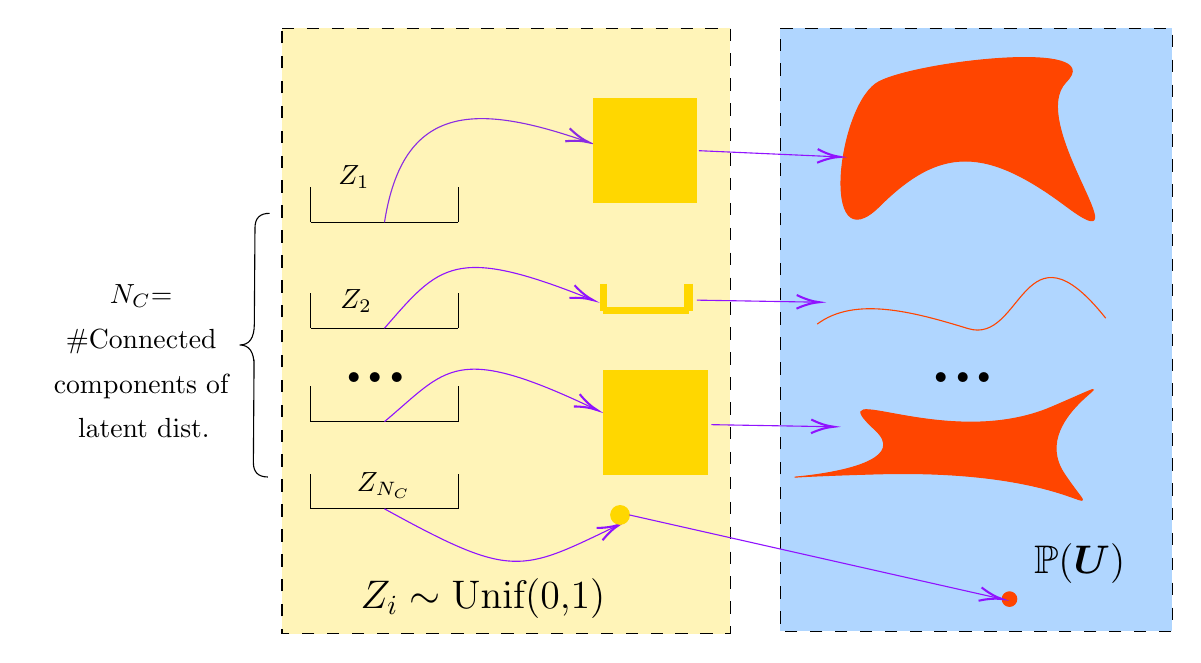
\begin{tikzpicture}[x=0.75pt,y=0.75pt,yscale=-1,xscale=1]
%uncomment if require: \path (0,335); %set diagram left start at 0, and has height of 335

%Shape: Rectangle [id:dp15930122249892342] 
\draw  [color={rgb, 255:red, 0; green, 0; blue, 0 }  ,draw opacity=1 ][fill={rgb, 255:red, 0; green, 123; blue, 255 }  ,fill opacity=0.31 ][dash pattern={on 4.5pt off 4.5pt}] (363.16,35.31) -- (552.02,35.31) -- (552.02,325.93) -- (363.16,325.93) -- cycle ;
%Shape: Rectangle [id:dp9986917405631817] 
\draw  [color={rgb, 255:red, 0; green, 0; blue, 0 }  ,draw opacity=1 ][fill={rgb, 255:red, 255; green, 215; blue, 0 }  ,fill opacity=0.28 ][dash pattern={on 4.5pt off 4.5pt}] (123.16,35.31) -- (339.02,35.31) -- (339.02,327.12) -- (123.16,327.12) -- cycle ;
%Straight Lines [id:da26489669286703244] 
\draw    (137.02,128.85) -- (208.02,128.85) ;
%Straight Lines [id:da9888477499089534] 
\draw    (137.02,128.85) -- (137.02,111.85) ;
%Straight Lines [id:da2730093828070803] 
\draw    (208.02,128.85) -- (208.02,111.85) ;
%Straight Lines [id:da5717948289754777] 
\draw    (137.02,179.85) -- (208.02,179.85) ;
%Straight Lines [id:da5953442554223825] 
\draw    (137.02,179.85) -- (137.02,162.85) ;
%Straight Lines [id:da6324631776083152] 
\draw    (208.02,179.85) -- (208.02,162.85) ;
%Straight Lines [id:da8348154802152368] 
\draw    (137.02,224.85) -- (208.02,224.85) ;
%Straight Lines [id:da5026006821299596] 
\draw    (137.02,224.85) -- (137.02,207.85) ;
%Straight Lines [id:da5989217517467482] 
\draw    (208.02,224.85) -- (208.02,207.85) ;
%Straight Lines [id:da8194431543259233] 
\draw    (137.02,266.85) -- (208.02,266.85) ;
%Straight Lines [id:da3884338087659025] 
\draw    (137.02,266.85) -- (137.02,249.85) ;
%Straight Lines [id:da5105817541521418] 
\draw    (208.02,266.85) -- (208.02,249.85) ;
%Shape: Polygon Curved [id:ds050110039454926314] 
\draw  [color={rgb, 255:red, 255; green, 69; blue, 0 }  ,draw opacity=1 ][fill={rgb, 255:red, 255; green, 69; blue, 0 }  ,fill opacity=1 ] (411,61) .. controls (431,51) and (521,41) .. (501,61) .. controls (481,81) and (539.98,150.15) .. (501,121) .. controls (462.02,91.85) and (439.98,92.15) .. (411,121) .. controls (382.02,149.85) and (391,71) .. (411,61) -- cycle ;
%Curve Lines [id:da2609994038248238] 
\draw [color={rgb, 255:red, 255; green, 69; blue, 0 }  ,draw opacity=1 ]   (381.02,177.85) .. controls (398.99,164.37) and (427.26,171.89) .. (453.67,180.01) .. controls (480.07,188.12) and (480.02,124.7) .. (520,175) ;
%Shape: Circle [id:dp047849516898298416] 
\draw  [color={rgb, 255:red, 255; green, 69; blue, 0 }  ,draw opacity=1 ][fill={rgb, 255:red, 255; green, 69; blue, 0 }  ,fill opacity=1 ] (470.15,310.35) .. controls (470.15,308.42) and (471.71,306.85) .. (473.65,306.85) .. controls (475.58,306.85) and (477.15,308.42) .. (477.15,310.35) .. controls (477.15,312.29) and (475.58,313.85) .. (473.65,313.85) .. controls (471.71,313.85) and (470.15,312.29) .. (470.15,310.35) -- cycle ;
%Curve Lines [id:da37224530912069054] 
\draw [color={rgb, 255:red, 138; green, 43; blue, 226 }  ,draw opacity=1 ]   (172.52,128.85) .. controls (181.43,71.43) and (216.31,71.31) .. (269.4,89.75) ;
\draw [shift={(271.02,90.31)}, rotate = 199.38] [color={rgb, 255:red, 138; green, 43; blue, 226 }  ,draw opacity=1 ][line width=0.75]    (10.93,-3.29) .. controls (6.95,-1.4) and (3.31,-0.3) .. (0,0) .. controls (3.31,0.3) and (6.95,1.4) .. (10.93,3.29)   ;
%Curve Lines [id:da8010124660438036] 
\draw [color={rgb, 255:red, 144; green, 19; blue, 254 }  ,draw opacity=1 ]   (172.52,266.85) .. controls (234.39,300.97) and (237.95,297.39) .. (284.59,275) ;
\draw [shift={(286.02,274.31)}, rotate = 154.4] [color={rgb, 255:red, 144; green, 19; blue, 254 }  ,draw opacity=1 ][line width=0.75]    (10.93,-3.29) .. controls (6.95,-1.4) and (3.31,-0.3) .. (0,0) .. controls (3.31,0.3) and (6.95,1.4) .. (10.93,3.29)   ;
%Curve Lines [id:da2374364900264201] 
\draw [color={rgb, 255:red, 144; green, 19; blue, 254 }  ,draw opacity=1 ]   (172.52,179.85) .. controls (199.02,149.41) and (206.09,139.36) .. (272.02,165.91) ;
\draw [shift={(273.02,166.31)}, rotate = 202.03] [color={rgb, 255:red, 144; green, 19; blue, 254 }  ,draw opacity=1 ][line width=0.75]    (10.93,-3.29) .. controls (6.95,-1.4) and (3.31,-0.3) .. (0,0) .. controls (3.31,0.3) and (6.95,1.4) .. (10.93,3.29)   ;
%Shape: Polygon Curved [id:ds2277785699514534] 
\draw  [color={rgb, 255:red, 255; green, 69; blue, 0 }  ,draw opacity=1 ][fill={rgb, 255:red, 255; green, 69; blue, 0 }  ,fill opacity=1 ] (409.02,228.85) .. controls (381.02,202.85) and (443.04,239.71) .. (494.02,217.85) .. controls (545,196) and (480,220) .. (500,250) .. controls (520,280) and (511.98,247.15) .. (410,250) .. controls (308.02,252.85) and (437.02,254.85) .. (409.02,228.85) -- cycle ;
%Curve Lines [id:da8327407583075901] 
\draw [color={rgb, 255:red, 144; green, 19; blue, 254 }  ,draw opacity=1 ]   (172.52,224.85) .. controls (202.87,199.44) and (206.12,186.39) .. (273.99,218.82) ;
\draw [shift={(275.02,219.31)}, rotate = 205.64] [color={rgb, 255:red, 144; green, 19; blue, 254 }  ,draw opacity=1 ][line width=0.75]    (10.93,-3.29) .. controls (6.95,-1.4) and (3.31,-0.3) .. (0,0) .. controls (3.31,0.3) and (6.95,1.4) .. (10.93,3.29)   ;
%Shape: Square [id:dp7698616097738606] 
\draw  [color={rgb, 255:red, 255; green, 215; blue, 0 }  ,draw opacity=1 ][fill={rgb, 255:red, 255; green, 215; blue, 0 }  ,fill opacity=1 ] (273.02,69.31) -- (323.02,69.31) -- (323.02,119.31) -- (273.02,119.31) -- cycle ;
%Shape: Square [id:dp47706693737043326] 
\draw  [color={rgb, 255:red, 255; green, 215; blue, 0 }  ,draw opacity=1 ][fill={rgb, 255:red, 255; green, 215; blue, 0 }  ,fill opacity=1 ] (278.02,200.31) -- (328.02,200.31) -- (328.02,250.31) -- (278.02,250.31) -- cycle ;
%Shape: Circle [id:dp003438441013369875] 
\draw  [color={rgb, 255:red, 255; green, 215; blue, 0 }  ,draw opacity=1 ][fill={rgb, 255:red, 255; green, 215; blue, 0 }  ,fill opacity=1 ] (281.52,269.81) .. controls (281.52,267.33) and (283.53,265.31) .. (286.02,265.31) .. controls (288.5,265.31) and (290.52,267.33) .. (290.52,269.81) .. controls (290.52,272.3) and (288.5,274.31) .. (286.02,274.31) .. controls (283.53,274.31) and (281.52,272.3) .. (281.52,269.81) -- cycle ;
%Straight Lines [id:da2344664098443705] 
\draw [color={rgb, 255:red, 255; green, 215; blue, 0 }  ,draw opacity=1 ][line width=2.25]    (278.02,171.31) -- (319.02,171.31) ;
%Straight Lines [id:da6947502424292837] 
\draw [color={rgb, 255:red, 255; green, 215; blue, 0 }  ,draw opacity=1 ][line width=2.25]    (278.02,158.31) -- (278.02,171.31) ;
%Straight Lines [id:da20815314130597984] 
\draw [color={rgb, 255:red, 255; green, 215; blue, 0 }  ,draw opacity=1 ][line width=3]    (319.02,158.31) -- (319.02,171.31) ;
%Straight Lines [id:da2895948921678664] 
\draw [color={rgb, 255:red, 144; green, 19; blue, 254 }  ,draw opacity=1 ]   (324.02,94.31) -- (390.02,97.23) ;
\draw [shift={(392.02,97.31)}, rotate = 182.53] [color={rgb, 255:red, 144; green, 19; blue, 254 }  ,draw opacity=1 ][line width=0.75]    (10.93,-3.29) .. controls (6.95,-1.4) and (3.31,-0.3) .. (0,0) .. controls (3.31,0.3) and (6.95,1.4) .. (10.93,3.29)   ;
%Straight Lines [id:da9851760758564494] 
\draw [color={rgb, 255:red, 144; green, 19; blue, 254 }  ,draw opacity=1 ]   (323.02,166.31) -- (380.02,167.28) ;
\draw [shift={(382.02,167.31)}, rotate = 180.97] [color={rgb, 255:red, 144; green, 19; blue, 254 }  ,draw opacity=1 ][line width=0.75]    (10.93,-3.29) .. controls (6.95,-1.4) and (3.31,-0.3) .. (0,0) .. controls (3.31,0.3) and (6.95,1.4) .. (10.93,3.29)   ;
%Straight Lines [id:da04661030541261035] 
\draw [color={rgb, 255:red, 144; green, 19; blue, 254 }  ,draw opacity=1 ]   (330.02,226.31) -- (387.02,227.28) ;
\draw [shift={(389.02,227.31)}, rotate = 180.97] [color={rgb, 255:red, 144; green, 19; blue, 254 }  ,draw opacity=1 ][line width=0.75]    (10.93,-3.29) .. controls (6.95,-1.4) and (3.31,-0.3) .. (0,0) .. controls (3.31,0.3) and (6.95,1.4) .. (10.93,3.29)   ;
%Straight Lines [id:da11563606750531141] 
\draw [color={rgb, 255:red, 144; green, 19; blue, 254 }  ,draw opacity=1 ]   (290.52,269.81) -- (468.2,309.91) ;
\draw [shift={(470.15,310.35)}, rotate = 192.72] [color={rgb, 255:red, 144; green, 19; blue, 254 }  ,draw opacity=1 ][line width=0.75]    (10.93,-3.29) .. controls (6.95,-1.4) and (3.31,-0.3) .. (0,0) .. controls (3.31,0.3) and (6.95,1.4) .. (10.93,3.29)   ;
%Shape: Brace [id:dp7095582501561211] 
\draw  [color={rgb, 255:red, 0; green, 0; blue, 0 }  ,draw opacity=1 ] (117.17,124.5) .. controls (112.5,124.47) and (110.16,126.78) .. (110.13,131.45) -- (109.81,177.96) .. controls (109.76,184.63) and (107.41,187.94) .. (102.74,187.91) .. controls (107.41,187.94) and (109.72,191.29) .. (109.67,197.96)(109.69,194.96) -- (109.36,244.48) .. controls (109.33,249.15) and (111.64,251.49) .. (116.31,251.52) ;

% Text Node
\draw (510.01,293.35) node  [font=\Large] [align=left] {\begin{minipage}[lt]{36.73pt}\setlength\topsep{0pt}
$\displaystyle \mathbb{P}(\boldsymbol{U})$
\end{minipage}};
% Text Node
\draw (220,310) node  [font=\Large] [align=left] {$\displaystyle Z_{i} \sim \text{Unif(0,1)}$};
% Text Node
\draw (55.29,195.72) node   [align=left] {\begin{minipage}[lt]{75.35pt}\setlength\topsep{0pt}
\begin{center}
$\displaystyle N_{C}$= \#Connected components of latent dist. 
\end{center}

\end{minipage}};
% Text Node
\draw (149,100) node [anchor=north west][inner sep=0.75pt]    {$Z_{1}$};
% Text Node
\draw (150,160) node [anchor=north west][inner sep=0.75pt]    {$Z_{2}$};
% Text Node
\draw (158,248) node [anchor=north west][inner sep=0.75pt]    {$Z_{N_{C}}$};
% Text Node
\draw (151.39,200) node [anchor=north west][inner sep=0.75pt]   [align=left] {\textbf{{\Huge ...}}};
% Text Node
\draw (434.39,200) node [anchor=north west][inner sep=0.75pt]   [align=left] {\textbf{{\Huge ...}}};
\end{tikzpicture}
}
\caption{ This figure demonstrates the first two parts of our architecture. Each interval in the yellow box corresponds to one coordinate of input in the left figure. We first push forward uniform distributions to different cubes. Then, using \cref{assump:support}, we adapt the shape of the support and push the measure from unit cubes to the original support of $P(\boldsymbol{U})$. In this way, we can approximate complicated measures by pushing forward uniform variables. }
\label{fig:pf-2}
\end{minipage}
\end{figure}

\noindent\textit{Remark (notation).} $N_C$ denotes the finite number of connected components of $\operatorname{supp}(\mathbb P)$, indexed by $i\in[N_C]$. In Theorem~\ref{thm:consistency}, Corollary~\ref{cor:rate}: The finite component count of each latent generator architecture in $\mathcal F_{1,n}$ is fixed as $n$ varies.



In this subsection, we will extend the results in \cite{perekrestenkoHighDimensionalDistributionGeneration2022a} to construct a neural network as the push-forward map. It turns out that to get a good approximation of the targeted distribution, the shape of the support is essential. We introduce the following two assumptions for our latent distribution.
\begin{assumption}[Mixed Distribution]\label{assump:support}
    The support of measure $ \mathbb{P}$ has finite connected components $ C_{1} ,C_{2} \cdots C_{N_C} $, i.e., $ {\text{supp}(\mathbb{P})} =\bigcup _{i=1}^{N_C} C_{i}$, and each component $ C_{i}$ satisfies $\mathcal{H}([0,1]^{d^C_i},C_i) \cap \mathcal{F}_L([0,1]^{d^C_i},C_i) \neq \emptyset$ for some $d_i^C \geqslant 0$. Recall that $\mathcal{H}(K_1,K_2)$ is the set of homeomorphisms from $K_1$ to $K_2$ defined at the end of  \cref{sec:preliminary}. 
\end{assumption}

\noindent\textit{Remark (notation).} For $i\in[N_C]$, $d_i^C$ is a nonnegative integer such that $\mathcal{H}([0,1]^{d_i^C},C_i)\cap\mathcal{F}_L([0,1]^{d_i^C},C_i)\neq\emptyset$; $d_i^C=0$ corresponds to a singleton component. In Theorem~\ref{thm:consistency}, Corollary~\ref{cor:rate}: The component cube dimensions of each latent generator architecture in $\mathcal F_{1,n}$ are fixed as $n$ varies.

 \cref{assump:support} encompasses almost all natural distributions. For example, distributions supported on $ [0,1]^d $ and closed balls, finitely supported distributions and mixtures of them all satisfy this assumption. \cref{assump:support} allows us to transform the support of the targeted distribution into unit cubes and the nice geometric properties of unit cubes facilitate our construction. The next assumption is slightly than \cref{assump:support}, but we will show later that it can give us a better rate.\par   

\begin{assumption}[Lower Bound]\label{assumption:lower_bound}
Suppose that $ \mathbb{P}$ is supported on a compact set $ K\subset \mathbb{R}^{D}$, there exists a constant $ C_{f}  >0$, $ f\in \mathcal{H}([0,1]^{d},K) \cap \mathcal{F}_L([0,1]^{d},K)$,  such that for any measurable set $ B\subset [ 0,1]^{d}$, $ \mathbb{P}\left( f( B)\right) \geqslant C_{f} \lambda ( B)$. Besides, if $d>0$, $(f^{-1})_{\#}\mathbb P$ vanishes on the boundary $\partial[0,1]^d$.
\end{assumption}

\noindent\textit{Remark (notation).} $C_f$ is a positive domination constant associated with the particular measure $\mathbb{P}$ and chosen homeomorphism $f$ in the lower-bound assumption.

\cref{assumption:lower_bound} implies that $d \lambda /d (f^{-1}_{\#}\mathbb{P})$ exists and is lowered bounded by a constant $C_f$. We show in the appendix (\cref{prop:holder_curve}) that under \cref{assumption:lower_bound}, it is possible to simulate any distribution on the unit cubes with Hölder continuous curves and uniform distribution on $ [ 0,1]$. \cref{prop:holder_curve} can be viewed as an extension of the Skorohod representation theorem. 

Now, we briefly explain the construction of the push-forward maps. An example is provided in \cref{sec:nn_example} to illustrate the construction. The NN architecture consists of three parts (see \cref{fig:wide_nn}). The input dimension is the same as the number of connected components of the support $ N_C $. For each component $ C_i $, let $ H_i\in \mathcal{H}([0,1]^{d^C_i},C_i) \cap \mathcal{F}_L([0,1]^{d^C_i},C_i) $, where $d_i^C$ is the dimension of component $C_i$ in \cref{assump:support}. By $ \mathbb{P} = (H_i)_{\#}(H_i^{-1})_{\#} \mathbb{P} $ on $ C_i $, we can approximate $ (H_i^{-1})_{\#} \mathbb{P} $ first, which is supported on a unit cube. \cite{perekrestenkoHighDimensionalDistributionGeneration2022a} constructs a wide NN $ \hat{g}$ of width $ W $ and constant depth such that $ W(\hat{g}_{\#} \lambda,(H_i)^{-1}_{\#}\mathbb{P})\leqslant O(W^{-1/d_i^C}) $ where $ \lambda $ is the uniform measure on $ [0,1] $. Then, we approximate the Lipschitz map $ H_i $ to $C_i$ to pull the distribution back to $ C_i $. These are the first two parts (yellow and blue blocks in \cref{fig:wide_nn}) of the architecture. \par 

Suppose that the output of $i$-th coordinate in the first two parts is $ \Vec{v}_i $, the Gumbel-softmax layer in the third part (green box) combines different components of the support. In particular, we want to output $ \Vec{v}_i $ with probability $ p_i = \mathbb{P}(C_i) $. Let $ V = [\Vec{v}_1,\cdots,\Vec{v}_i] $, this can be achieved by outputting  $ V X $, where $ X = (X_1,\cdots,X_{N_C})^\mathsf{T}  $ is a one-hot random vector with $ \mathbb{P}({X}_i = 1) =  p_i$. To use backpropagation in training, we use the Gumbel-Softmax trick \cite{Jang2016CategoricalRW} to (approximately) simulate such a random vector, 
 $\hat{X}^\tau_i = \frac{\exp((\log p_i +G_i)/\tau)}{\sum_{k=1}^{N_C}\exp((\log p_k +G_k)/\tau)}, $
where $ \tau>0 $ is the temperature parameter (a hyperparameter) and $ G_i\sim \text{Gumbel}(0,1) $ are i.i.d. standard Gumbel variables. As $\tau \rightarrow 0$, the distribution of $\hat{X}^\tau$ converges almost surely to the categorical distribution \cite[Proposition 1]{maddisonConcreteDistributionContinuous2017}. In particular, when $ \tau = 0$, we denote $\hat{X}_i^0 = \mathbb{I}_{i = \arg\max_j \{\log p_i + G_i\}}$. The output of the last layer is $V\hat{X}^\tau$. Note that the Gumbel-softmax function is differentiable with respect to parameter $ \{\log (p_i)\}_{i=1,\cdots,N_C}$. Therefore, we can train the network with common gradient-based algorithms. 

\noindent\textit{Remark (notation).} $G_k$ is the $k$th standard Gumbel coordinate, with density $x\mapsto\exp(-x-\exp(-x))$ on $\mathbb{R}$, in the relevant Gumbel-softmax vector. In Lemma~\ref{lemma:gumbel_err}: The coordinate index is $k\in[n]$. In Theorem~\ref{thm:wide_nn}: $G_k$, $k\in[N_C]$, are the independent standard Gumbel coordinates of the mixing layer, one per connected support component, independent of the uniform inputs used by the deterministic blocks; their randomness is included in $\hat g_{\#}\lambda$. In the result split from Theorem~\ref{thm:wide_nn}: $G_k$, $k\in[N_C]$, are the independent standard Gumbel coordinates of the mixing layer, one per connected support component, independent of the uniform inputs used by the deterministic blocks; their randomness is included in $\hat g_{\#}\lambda$. $\tau>0$ is the Gumbel-softmax temperature hyperparameter; a superscript $0$ on a softmax output or layer denotes the limit as $\tau\rightarrow0$, rather than evaluation of the positive-temperature formula at zero. In Lemma~\ref{lemma:gumbel_err}: The temperature satisfies $0<\tau<1$. In Theorem~\ref{thm:wide_nn}: The error estimate is asymptotic as the network budgets tend to infinity and $\tau\downarrow0$, with constants independent of the budgets and $\tau$; the proof uses the Gumbel-softmax estimate for $0<\tau<1$. In Theorem~\ref{thm:consistency}: The temperature is the positive sequence $\tau_n$ appearing in $\mathcal{F}_{1,n}$, with $\tau_n\rightarrow0$. In the result split from Theorem~\ref{thm:wide_nn}: The error estimate is asymptotic as the network budgets tend to infinity and $\tau\downarrow0$, with constants independent of the budgets and $\tau$; the proof uses the Gumbel-softmax estimate for $0<\tau<1$. In Corollary~\ref{cor:rate}: The generator temperature is the positive sequence $\tau_n$ in $\mathcal F_{1,n}$ and in the approximation term $\tau_n(1-\log\tau_n)$. In Corollary~\ref{corollary:deep_nn}: The displayed error bound is asymptotic as $L_0,L_1,L_2\to\infty$ and $\tau\downarrow0$, with $R>0$ and the causal model fixed. The implicit constant is independent of the intervention and the network budgets, but may depend on $R$ and the fixed causal model.


In summary, our construction has the form $ \hat{g} =\hat{g}_{3}^{\tau } \circ \hat{g}_{2} \circ \hat{g}_{1} $, where $ \hat{g}_{i} ,i=1,2$ have the separable form $ \left(\hat{g}_{i}^{1}( x_{1}) ,\cdots ,\hat{g}_{i}^{N_{C}}( x_{N_{C}})\right)$ and $ \hat{g}_{1}^{j} \in \mathcal{NN}_{1,d_j^C}( W_{1} , L_1)$, $ \ \hat{g}_{2}^{j} \in \mathcal{NN}_{d_j^C,d}(W_2 ,L_{2}) ,\ j\in [ N_{C}]$; $ \{d_j^C\} $ are the dimension of cubes in \cref{assump:support}. $ \hat{g}_{3}^{\tau }$ is the Gumbel-Softmax layer with temperature parameter $ \tau>0 $. We slightly abuse the notations and denote this class of neural nets by  $\mathcal{NN}(W_1,L_1,W_2,L_2,\tau) $. Putting things together, we obtain the following theorem.
\begin{theorem}\label{thm:wide_nn}
Given any probability measure $\mathbb P$ on $\mathbb R^d$ that satisfies \cref{assump:support}, let $\lambda$ be the Lebesgue measure on $[0,1]^{N_C}$, where $N_C$ is defined in \cref{assump:support}. Write $D_C=\max\{1,\max_i d_i^C\}$. 
  \begin{enumerate}
\item There exists a neural network $\hat g\in\mathcal{NN}(W_1,\Theta(D_C),\Theta(d\cdot D_C),L_2,\tau)$ with the above architecture (\cref{fig:wide_nn}) such that
\begin{equation*}
W(\hat g_{\#}\lambda,\mathbb P)\leqslant O\left(\mathbb I_{\{\max_i d_i^C>0\}}\left(W_1^{-1/D_C}+L_2^{-2/D_C}\right)+(\tau-\tau\log\tau)\right).
\end{equation*}
\end{enumerate}
\end{theorem}

\noindent\textit{Remark.} A network in $\mathcal{NN}_{k_1,k_2}(W,L)$ has $L$ hidden layers, each of width at most $W$, followed by the affine output layer (width at most $W$ and exactly $W$ give the same class of functions: a narrower layer is padded with zero units). The covering number $\mathcal{N}(\epsilon,S,\|\cdot\|_1)$ is that of the cited source (Anthony and Bartlett): the least size of a subset $C\subseteq S$ such that every point of $S$ lies at $\ell_1$ distance strictly less than $\epsilon$ from some point of $C$. The law $\hat g_{\#}\lambda$ includes the independent standard Gumbel variables used in the mixing layer. The error estimates are asymptotic as the network budgets tend to infinity and $\tau\downarrow0$, with constants independent of these budgets and of $\tau$. A component with $d_i^C=0$ is a singleton, and its two deterministic blocks are the unique map to $[0,1]^0$ and a constant affine map to that singleton. In the proposition entitled ``Deep distribution approximation'', the multiplicative width factors in $\Theta(D_C)$ and $\Theta(dD_C)$ are absolute numerical constants, independent of the measure, chart constants, dimensions, and component count. $f\in\mathcal{H}(K_1,K_2)$ means that $f:K_1\rightarrow K_2$ is bijective and both $f$ and $f^{-1}:K_2\rightarrow K_1$ are continuous. A network in $\mathcal{NN}_{k_1,k_2}(W,L)$ has $L$ hidden ReLU layers of width at most $W$, followed by an affine output layer of dimension $k_2$. The layer uses $V=[\Vec{v}_1,\ldots,\Vec{v}_{N_C}]$ and the same Gumbel draws for all $\tau>0$, with $\lim_{\tau\downarrow0}\hat{X}^{\tau}_i=\hat{X}^{0}_i=\mathbb{I}_{\{i=\arg\max_{j\in[N_C]}(\log p_j+G_j)\}}$ almost surely for every $i\in[N_C]$. For each component of positive dimension $q=d_i^C$, the application of Theorem VIII.1 of \cite{perekrestenkoHighDimensionalDistributionGeneration2022a} uses integer depth parameter $s=1$, quantization parameter $\delta=1/\lceil\sqrt q(q+1)n(n-1)\rceil$, and quantization mesh $\delta/n$. The refinement integer is $n=\lfloor(W_1/A_q)^{1/q}\rfloor$ for $W_1\geqslant A_q2^q$, where $A_q\geqslant1$ depends only on $q$ and bounds the clipped network width by $A_qn^q$.

\noindent\textit{Remark (notation).} This is the three-part generator class with component count $N_C$, component cube dimensions $d_j^C$, and output dimension $d$ suppressed from its arguments; $W_1,L_1$ and $W_2,L_2$ specify the respective component-network widths and depths, and $\tau>0$ specifies the mixing temperature. In Corollary~\ref{corollary:deep_nn}: The four-argument generator-class occurrence suppresses the temperature argument; the latent generators retain the Gumbel-softmax temperature $\tau$ appearing in the bound. The multiplicative width factors in $\Theta(d_{\max}^U)$ and $\Theta((d_{\max}^U)^2)$ can be chosen as absolute numerical constants, independent of the causal model, $R$, all dimensions, and all category and component counts. In Theorem~\ref{thm:consistency}: The class used is its truncated version $\mathcal{NN}^{\infty,K}(\Theta(d_{\max}^U),L_{1,n},\Theta((d_{\max}^U)^2),L_{2,n},\tau_n)$; the superscript $\infty$ imposes no finite Lipschitz bound, while $K$ specifies coordinatewise output truncation, and the finite component counts and component cube dimensions of the latent generator architectures are fixed as $n$ varies. In Theorem~\ref{thm:wide_nn}, the result split from Theorem~\ref{thm:wide_nn}: The architecture includes components with $d_i^C=0$: their first deterministic block is the unique map to $[0,1]^0$, and their second deterministic block is a constant affine map to the corresponding singleton. In Corollary~\ref{cor:rate}: The latent generator class is the truncated class $\mathcal F_{1,n}=\mathcal{NN}^{\infty,K}(\Theta(d_{\max}^U),L_{1,n},\Theta((d_{\max}^U)^2),L_{2,n},\tau_n)$; the superscript $\infty$ imposes no finite Lipschitz bound, $K$ specifies coordinatewise output truncation, and the finite component counts and component cube dimensions are fixed as $n$ varies. In the result split from Theorem~\ref{thm:wide_nn}: The multiplicative width factors in $\Theta(D_C)$ and $\Theta(dD_C)$ are absolute numerical constants, independent of the measure, chart constants, dimensions, and component count. Each coordinate block $\hat{g}_1^j$ uses one scalar input to generate coordinates in the cube $[0,1]^{d_j^C}$ associated with component $j$, without mixing inputs from different components. In Theorem~\ref{thm:wide_nn}, the result split from Theorem~\ref{thm:wide_nn}: Writing $\mu_j=\mathbb{P}_{C_j}/\mathbb{P}(C_j)$, for $d_j^C\geqslant1$ the first block approximates the cube law $((g_2^j)^{-1})_{\#}\mu_j$ by the law of $\hat{g}_1^j(U_j)$; for $d_j^C=0$, it is the unique map to $[0,1]^0$. Each coordinate block $\hat{g}_2^j$ maps the $d_j^C$-dimensional cube coordinates for component $j$ into $\mathbb{R}^d$, without mixing inputs from different components. In Theorem~\ref{thm:wide_nn}, the result split from Theorem~\ref{thm:wide_nn}: For $d_j^C\geqslant1$, the block $\hat{g}_2^j$ approximates a map $g_2^j\in\mathcal{H}([0,1]^{d_j^C},C_j)\cap\mathcal{F}_L([0,1]^{d_j^C},C_j)$; for $d_j^C=0$, it is a constant affine map to the singleton $C_j$. $\hat{g}_3^\tau$ mixes the $N_C$ component outputs using the Gumbel-softmax coefficient vector, with $\tau>0$; the notation $\hat{g}_3^0$ denotes its almost-sure hard-selection limit as $\tau\rightarrow0$. In Theorem~\ref{thm:wide_nn}: The mixing weights are $p_k=\mathbb{P}(C_k)$ for the connected components $C_k$ of the target support. In Corollary~\ref{corollary:deep_nn}: The layer is used separately for each latent generator, with mixing weights given by the masses of the connected components of that latent variable's target law. In Theorem~\ref{thm:consistency}: At sample size $n$, the generator class uses temperature $\tau_n>0$ and truncates the resulting generator output coordinatewise to $[-K,K]$. In the result split from Theorem~\ref{thm:wide_nn}: The mixing weights are $p_k=\mathbb{P}(C_k)$ for the connected components $C_k$ of the target support.

\begin{corollary}[Deep distribution approximation]\label{thm:cor-fix-3c402872}
Given any probability measure $\mathbb P$ on $\mathbb R^d$ that satisfies \cref{assump:support}, let $\lambda$ be the Lebesgue measure on $[0,1]^{N_C}$, where $N_C$ is defined in \cref{assump:support}, and write $D_C=\max\{1,\max_i d_i^C\}$. Suppose in addition that $\mathbb P$ constrained to each component satisfies \cref{assumption:lower_bound}. There exists a neural network $\hat g\in\mathcal{NN}(\Theta(D_C),L_1,\Theta(d\cdot D_C),L_2,\tau)$ with the architecture of \cref{fig:wide_nn} such that

\[
W(\hat g_{\#}\lambda,\mathbb P)\leqslant O\left(\mathbb I_{\{\max_i d_i^C>0\}}\left(L_1^{-2/D_C}+L_2^{-2/D_C}\right)+(\tau-\tau\log\tau)\right).
\]
\end{corollary}


Note that $\hat{g}^\tau_3$ (the Gumbel-softmax layer) is actually a random function since the coefficient vector $\hat{X}^\tau$ is a random variable. In this sense, $\hat{g}_{\#} \lambda$ can be viewed as pushing forward uniform and Gumbel variables using a neural net. 

The second conclusion of \cref{thm:wide_nn} shows that under one additional assumption on the distribution, deep ReLU networks have a stronger approximation power in approximating distributions, which means we can use fewer computational units to achieve the same worst-case theoretical approximation error. 

\subsection{NCM Construction}\label{sec:ncm_const}
Now, we can use the previous distribution approximation results to construct NCM approximations. For simplicity, we omit the input and output dimensions of the neural network. As we mention in previous sections, our construction (\ref{eq:structure_equation_hat}) consists of two parts, $ \hat{f}_{i}$ approximating the structural functions $f_i$ in (\ref{eq:structure_equation}), and $ \hat{g}_{j}(Z_j) $ approximating the latent variables $U_j$. Let $ \text{NCM}_{\mathcal{G}}(\mathcal{F}_0,\mathcal{F}_1)$ be a collection of NCMs with structural equation (\ref{eq:structure_equation_hat}) and $ \hat{f}_{i} \in \mathcal{F}_0, \hat{g} \in \mathcal{F}_1. $ 
By combining \cref{thm:approximation} and \cref{thm:wide_nn}, we have the following corollary. 

\noindent\textit{Remark (notation).} $\text{NCM}_{\mathcal{G}}(\mathcal{F}_0,\mathcal{F}_1)$ is the collection of models on $\mathcal{G}$ with structural equations (\ref{eq:structure_equation_hat}), in which every structural network belongs to $\mathcal{F}_0$ and every component-specific latent generator belongs to $\mathcal{F}_1$, with compatible dimensions suppressed. In Theorem~\ref{thm:consistency}, Corollary~\ref{cor:rate}: At sample size $n$, the candidate class is $\text{NCM}_{\mathcal G}(\mathcal F_{0,n},\mathcal F_{1,n})$, with the architecture and truncation specified in Theorem~\ref{thm:consistency}, restricted so that every categorical raw structural network $q$ satisfies $q(x)\in[0,\infty)^{n_i}$, $\|q(x)\|_1>0$ for every structural input $x$, and $\operatorname{Lip}(x\mapsto q(x)/\|q(x)\|_1)\leqslant\hat L_f$. In Theorem~\ref{thm:consistency}: The empirical optimization ranges over network representations in the restricted candidate class; representations with the same latent population laws remain distinct candidates and may yield different common-draw empirical distributions. Every admitted continuous structural network additionally satisfies $\sup_x\|\hat f_i(x)\|_1\leqslant K$ on its full structural input domain. In Corollary~\ref{cor:rate}: Candidates are evaluated as network representations on the same $m_n$ exogenous simulation draws; representations with identical latent population laws can yield different empirical distributions on these common draws. Every admitted continuous structural network additionally satisfies $\sup_x\|\hat f_i(x)\|_1\leqslant K$ on its full structural input domain. $\mathcal{F}_0$ is the structural-network class supplied to $\text{NCM}_{\mathcal{G}}(\mathcal{F}_0,\mathcal{F}_1)$, with the input and output dimensions appropriate to each node omitted from the notation. In Theorem~\ref{thm:consistency}: The class is $\mathcal{F}_{0,n}=\mathcal{NN}^{\hat L_f,K}(W_{0,n},\Theta(\log d_{\max}^{\text{in}}))$, where $\hat L_f=\sqrt{d_{\max}^{\text{in}}d_{\max}^{\text{out}}}L_f$; it consists of coordinatewise truncations to $[-K,K]$ of networks whose Lipschitz constant is at most $\hat L_f$, and varies with $n$. When $d_{\max}^{\text{in}}=1$, the depth expression uses $\Theta(1+\log d_{\max}^{\text{in}})$. Continuous structural networks admitted to the optimization additionally satisfy $\sup_x\|\hat f_i(x)\|_1\leqslant K$ on their full structural input domains. Categorical raw networks admitted to the optimization additionally satisfy $q(x)\in[0,\infty)^{n_i}$, $\|q(x)\|_1>0$ for every structural input $x$, and $\operatorname{Lip}(x\mapsto q(x)/\|q(x)\|_1)\leqslant\hat L_f$.


\begin{corollary}\label{corollary:deep_nn}
Given a causal model $\mathcal M^*\in\mathcal M(\mathcal G,\mathcal F_L,\boldsymbol U)$, suppose that Assumptions \ref{assump:independence_u}-\ref{assump:Lip_and_bounded} hold and the distributions of $U_C$ for all $C^2$-component satisfy the assumptions of the proposition entitled ``Deep distribution approximation''. Let $d_{\max}^{\text{in}}$ and $d_{\max}^{\text{out}}$ be the largest input and output dimension of $f_i$ in (\ref{eq:structure_equation}) and $d_{\max}^U$ be the largest dimension of all latent variables. Suppose in addition that $d_{\max}^{\text{in}}>0$ and $d_{\max}^U>0$. Fix any $R>0$. There exists a neural causal model 
  $$\hat{\mathcal{M}} \in \text{NCM}_{\mathcal{G}} ( \mathcal{NN}(\Theta( d^{\text{in}}_{\max}d^{\text{out}}_{\max}) ,L_{0}) , \mathcal{NN}(\Theta(d_{\max}^U),L_1,\Theta((d_{\max}^U)^2),L_2))$$ with structure equations (\ref{eq:structure_equation_hat}). For any intervention $\boldsymbol{T}=\boldsymbol{t}$ such that $\|t_i\|_\infty\leqslant R$ for each continuous treatment variable $T_i$, $\hat{\mathcal M}$ satisfies
\begin{equation*}
W\left(P^{\mathcal M^*}(\boldsymbol V(\boldsymbol t)),P^{\hat{\mathcal M}}(\boldsymbol V(\boldsymbol t))\right)\leqslant O\left(L_0^{-2/d_{\max}^{\text{in}}}+L_1^{-2/d_{\max}^U}+L_2^{-2/d_{\max}^U}+(\tau-\tau\log\tau)\right).
\end{equation*}
The implicit constant is independent of the intervention and the network budgets, but may depend on $R$ and the fixed causal model.

\emph{Additional condition.} In the categorical structural equations, $\arg\max$ selects the smallest maximizing label when there is a tie. This is a measurable completion on ties; under the stipulated independent standard Gumbel noises and nonnegative propensity weights of positive total, it leaves every fixed-intervention law unchanged.
\end{corollary}

\noindent\textit{Remark.} In Corollary~\ref{corollary:deep_nn}, for $m_i=d_i^{\text{in}}>0$, the symbol $\hat f_i$ denotes $q_i\circ\Pi_i$ for a continuous variable and the vector $\bigl(\max\{\epsilon_i,(q_i\circ\Pi_i)_k\}\bigr)_{k=1}^{n_i}$ for a categorical variable, where $q_i$, $\Pi_i$, and $\epsilon_i=A_iL_0^{-2/m_i}$ are chosen in its proof. In Corollary~\ref{corollary:deep_nn}, for $m_i=0$, the symbol $\hat f_i$ denotes the exact constant function $f_i$. The error estimate is asymptotic as $L_0,L_1,L_2\to\infty$ and $\tau\downarrow0$, for fixed $R$ and fixed causal model. The latent generator class in the statement uses the same temperature $\tau$ as the displayed error estimate. The multiplicative width factors in $\Theta(d_{\max}^{\text{in}}d_{\max}^{\text{out}})$, $\Theta(d_{\max}^U)$, and $\Theta((d_{\max}^U)^2)$ can be chosen as absolute numerical constants, independent of the causal model, $R$, all dimensions, and all category and component counts. For each latent law $P(U_C)$, the assumptions of the proposition entitled ``Deep distribution approximation'' require the support charts of \cref{assump:support} and \cref{assumption:lower_bound} on each normalized component law $\mu_i=P(U_C)|_{C_i}/P(U_C\in C_i)$, with $(f^{-1})_{\#}\mu_i(\partial[0,1]^{d_i^C})=0$ when $d_i^C>0$. The phrase ``uniform cubes'' denotes the unit cube domains $[0,1]^m$ used for deterministic uniform function approximation; it imposes no uniform probability law on structural inputs. For each categorical $V_i$, the noise in equation (\ref{eq:structure_equation_hat}) satisfies $g_k=g_k^{V_i}$ for $k\in[n_i]$. Membership in $\text{NCM}_{\mathcal G}(\mathcal F_0,\mathcal F_1)$ requires $\hat f_i\in\mathcal F_0$ for every observed node and $\hat g_j\in\mathcal F_1$ for every latent component, with the compatible input and output dimensions understood separately for each network. $d_{\max}^U=\max_{j\in[n_U]}d_j^U$ ranges over non-Gumbel latent variables, while $d_{\max}^{\mathrm{in}}=\max_i d_i^{\mathrm{in}}$ and $d_{\max}^{\mathrm{out}}=\max_i d_i^{\mathrm{out}}$, with $d_i^{\mathrm{out}}=n_i$ for categorical nodes.

\noindent\textit{Remark (notation).} $d_{\max}^{\text{in}}=\max_{i\in[n_V]}d_i^{\text{in}}$, where $d_i^{\text{in}}$ is the input dimension of $f_i(\text{Pa}(V_i),\boldsymbol{U}_{V_i})$ in the canonical structural equations. In Theorem~\ref{thm:consistency}, Corollary~\ref{cor:rate}: $d_{\max}^{\text{in}}\geqslant1$; when $d_{\max}^{\text{in}}=1$, the structural-network depth expression $\Theta(\log d_{\max}^{\text{in}})$ means $\Theta(1+\log d_{\max}^{\text{in}})$. In Corollary~\ref{corollary:deep_nn}: $d_{\max}^{\text{in}}>0$. $d_{\max}^{\text{out}}=\max_{i\in[n_V]}d_i^{\text{out}}$, where $d_i^{\text{out}}=d_i$ for a continuous structural function and $d_i^{\text{out}}=n_i$ for a categorical propensity vector. $d_{\max}^U=\max_{j\in[n_U]}d_j^U$, where $d_j^U$ is the dimension of a canonical latent variable $U_j$ whose distribution is approximated by a generator, distinct from the separately supplied categorical Gumbel noises. In Theorem~\ref{thm:consistency}, Corollary~\ref{cor:rate}: $d_{\max}^U\geqslant1$; it remains the maximum individual non-Gumbel latent dimension, distinct from the total dimension $D_U=\sum_{j=1}^{n_U}d_j^U$ and $D=\max\{1,D_U\}$. In Corollary~\ref{corollary:deep_nn}: $d_{\max}^U>0$.

 Similar approximation results also hold for wide NN approximation (the first construction in \cref{thm:wide_nn}), as presented in \cref{sec:wide_nn}. The proof can be easily adapted to the wide NNs architecture. \cref{cor:rate} gives an explicit construction of NCM for a given SCM, which shows the expressivity of NCMs for SCM with mixed variables. This result can be viewed as a generalization of the expressivity result in \cite{xia2022neural}, but our construction is completely different from \cite{xia2022neural}.
 







\section{Consistency of Neural Causal Partial Identification}\label{sec:consistency}

In this section, we prove the consistency of the max/min optimization approach to partial identification. In the finite sample setting, we consider the following estimator $F_n$ of the optimal values of (\ref{prob:pid}).
\begin{align}
F_n = \argmin_{\hat{\mathcal{M}} \in \text{NCM}_{\mathcal{G}}(\mathcal{F}_{0,n} ,\mathcal{F}_{1,n} )} & \mathbb{E}_{t\sim \mu _{T}}\mathbb{E}_{\hat{\mathcal{M}}}[ F( V_{1}( t) ,\cdots ,V_{n_{V}}( t))] ,\label{eq:opt_empiri}\\
s.t.~~~ & S_{\lambda_n}(P_{m_n}^{\hat{\mathcal{M}}}(\boldsymbol{V}) ,P^{\mathcal{M}^*}_{n}(\boldsymbol{V}) )\leqslant \alpha _{n} , \notag
\end{align}
where $ P^{\mathcal{M}^*}_{n}, P_{m_n}^{\hat{\mathcal{M}}}  $ are the empirical distribution of $ P^{\mathcal{M}^*},P^{\hat{\mathcal{M}}}$ with sample size $n,m_n$, $\mu_T$ is a given measure, $S_\lambda(\cdot,\cdot)$ is the Sinkhorn distance and $\mathcal{F}_{i,n}$ will be specified later. For example, the counterfactual outcome $\mathbb{E}[Y(1)]$ is a special case of the objective. Our results can be easily generalized to any linear combination of objective functions of this form. We use the Sinkhorn distance because it can be computed efficiently in practice \cite{feydy2020geometric}. We want to study if $F_n$ is a good lower bound as $n \rightarrow \infty$. \par % Move equation (6) here.  
To match the observational distribution, we need to increase the width or depth of the NNs we use. As the sample size increases, the number of parameters also increases to infinity, which creates difficulty for our analysis. To obtain consistency, we need to regularize the functions while preserving their approximation power. Surprisingly, if we do not use any regularization, the following proposition implies that consistency may not hold even if the SCM is identifiable. 
\begin{proposition}[Informal, see Proposition~\ref{prop:counterexample_foral} for a formal version]\label{prop:counterexample} 
There exists a constant $c>0$ and an identifiable SCM $\mathcal{M}^*$ satisfying Assumptions \ref{assump:independence_u}-\ref{assumption:lower_bound} such that for any $\epsilon >0$, there exists an SCM $\mathcal{M}_\epsilon$ satisfying $W(P^{\mathcal{M}^*}(\boldsymbol{V}),P^{\mathcal{M}_\epsilon}(\boldsymbol{V})) \leq \epsilon $ and $|\text{ATE}_{\mathcal{M}^*} - \text{ATE}_{\mathcal{M}_\epsilon}| > c $.
Here, for each non-Gumbel latent law $\mathbb P$ with connected support components $C_i$, Assumption~\ref{assumption:lower_bound} is required of each normalized component law $\mathbb P|_{C_i}/\mathbb P(C_i)$, with $K=C_i$.

\emph{Additional condition.} In the categorical structural equations, $\arg\max$ selects the smallest maximizing label when there is a tie. This is a measurable completion on ties; under the stipulated independent standard Gumbel noises and nonnegative propensity weights of positive total, it leaves every fixed-intervention law unchanged.
\end{proposition}

\noindent\textit{Remark.} Identifiable means: every SCM $\mathcal M$ on the backdoor graph of Proposition~\ref{prop:counterexample_foral} whose latent variables are all independent (Assumption~\ref{assump:independence_u}) and with $P^{\mathcal M}(\boldsymbol V)=P^{\mathcal M^*}(\boldsymbol V)$ has $\text{ATE}_{\mathcal M}=\text{ATE}_{\mathcal M^*}$; the comparison models $\mathcal M_\epsilon$ have that same graph. Models whose latents are pairwise independent but jointly dependent are not on the graph in this sense.

\noindent\textit{Remark (notation).} $\mathcal{M}_\epsilon$ denotes an SCM chosen for each tolerance $\epsilon>0$ in the counterexample family, rather than a single model independent of $\epsilon$. In Proposition~\ref{prop:counterexample_foral}: $\mathcal{M}_\epsilon$ has the same causal graph as $\mathcal{M}^*$; in the proof it is supplied by $\mathcal{M}_\delta$ with $\delta>0$ small enough that $\delta/2\leqslant\epsilon$. $c$ denotes a locally specified scalar, categorical configuration, or real-valued function, according to its defining expression. In Proposition~\ref{prop:counterexample}, Proposition~\ref{prop:counterexample_foral}: $c>0$ is chosen together with $\mathcal{M}^*$ before quantifying over $\epsilon>0$, and is independent of $\epsilon$; it is a strict lower bound for $|\text{ATE}_{\mathcal{M}^*}-\text{ATE}_{\mathcal{M}_\epsilon}|$. In Lemma~\ref{lemma:sinkhorn_approx}: In the proof's final self-term calculation, $c=W_{1,\lambda}(\nu,\nu)$ is the entropy-regularized self-transport value, with $|c|\leqslant(1+2\log m)\lambda$; it is nonpositive under the specified entropy convention. In Lemma~\ref{lemma:sup_wasserstein}: $c>0$ is the concentration constant multiplying $n\epsilon^2$ in the negative term of the probability exponent; it depends only on $d,K$ and is independent of $n,\delta,\epsilon$. In Proposition~\ref{prop:Lip_ATE}: In the proof, $c(t)=\int\hat f_y(a,t)\nu_A(da)-\int\hat f_y(a,t)\mu_A(da)$ is the contribution from changing the observational marginal of $A$, with $\nu_A$ and $\mu_A$ the respective observational marginals. In Theorem~\ref{thm:consistency}: In the observational concentration argument, $c$ ranges over the fixed finite set of possible complete categorical label vectors: $p_c=P(C=c)$ and $\mu_c=P((U_1,\ldots,U_{n_U})\mid C=c)$, the latter being used for $p_c>0$. In Corollary~\ref{cor:rate}: In categorical types $(u,c)$ and conditioning expressions, $c$ is a complete categorical label vector, with $p_c=P(C=c)$ and $\mu_c=P((U_1,\ldots,U_{n_U})\mid C=c)$ for $p_c>0$. Separately, in the concentration exponent $-cC^2m_nr_n^2$, $c>0$ is a fixed concentration constant.

Here, $ \mathcal{M}^* $ is the ground-truth model and $\mathcal{M}_\epsilon$ are the models we use to approximate $\mathcal{M}^*$. \cref{prop:counterexample} implies that even if the observation distributions are close and the ground-truth model is identifiable, their ATEs can be far away, regardless of the sample size, which indicates that the method may not be consistent. We need some regularization on $\mathcal{M}_\epsilon$ to recover consistency. In particular, we find that regularizing the Lipschitz constant of the NN can help. Much work has been done to impose Lipschitz regularization during the training process \cite{cisse2017parseval,virmauxLipschitzRegularityDeep2018a,goukRegularisationNeuralNetworks2021,pauliTrainingRobustNeural2021,bungertCLIPCheapLipschitz2021}. We denote $ \text{Lip}( f)$ to be the Lipschitz constant of a function $ f$ and define the truncated Lipschitz NN class, 
\begin{equation*}
    \mathcal{NN}_{d_{1} ,d_{2}}^{{L_f},{K}}(W,L) =\left\{\max\{-K,\min\{f,K\}\}:f\in \mathcal{NN}_{d_{1} ,d_{2}}\left({W} ,L\right),\text{Lip}(f) \leqslant L_f\right\}.
\end{equation*}
 For simplicity, we omit the dimensions and use shorthand $  \mathcal{N}\mathcal{N}^{L_f,K}(W,L)$. Similarly, we also define the class  $\mathcal{NN}^{\infty,K}(W_1,L_1,W_2,L_2,\tau)$ as a truncated version of $\mathcal{NN}(W_1,L_1,W_2,L_2,\tau)$. The next theorem gives the consistency result of the min estimator. To state the theorem, we define $ F_{*} =\mathbb{E}_{t\sim \mu _{T}}\mathbb{E}_{\mathcal{M}^*}[ F( V_{1}( t) ,\cdots ,V_{n_{V}}( t))]$ to be the true value and $ \underline{F}^{L}$ to be the optimal value of the following optimization problem over SCMs with Lipschitz constant $L$.
\begin{align}
\underline{F}^{L} = \argmin_{\hat{\mathcal{M}} \in \mathcal{M}\left(\mathcal{G} ,\mathcal{F}^K_{L} ,\boldsymbol{U}\right), P(\boldsymbol{U})} & \mathbb{E}_{t\sim \mu _{T}}\mathbb{E}_{\hat{\mathcal{M}}}[ F( V_{1}( t) ,\cdots ,V_{n_{V}}( t))] , \label{eq:consistent_limiting}\\
s.t. & W( P^{\hat{\mathcal{M}}}(\boldsymbol{V}) ,P^{\mathcal{M}^*}(\boldsymbol{V})) =0,\notag 
\end{align}
where the minimum is taken over $\mathcal{M}\left(\mathcal{G} ,\mathcal{F}^K_{L} ,\boldsymbol{U}\right)$ with $\mathcal{F}^K_{L} = \{f: \|f\|\leqslant K, f \in \mathcal{F}_{L}\} $ and all latent distributions $P(\boldsymbol{U})$. Note that if $L$ is the Lipschitz bound $L_f$ that we assume on our structural functions, then $\underline{{F}}^L$ is the sharp lower bound. 
\begin{theorem}\label{thm:consistency}
    Let $ \mathcal{M^*}$ be any SCM satisfying the assumptions of Corollary \ref{corollary:deep_nn}. Suppose that the Lipschitz constant of functions in $\mathcal{M}$ is $L_f$, $F:\mathbb{R}^{n_V}\rightarrow\mathbb{R}$ in (\ref{eq:opt_empiri}) is Lipschitz continuous and $\tau_n>0$, let $K>0$ be the constant in \cref{assump:Lip_and_bounded}, $\hat L_f=\sqrt{d_{\max}^{\text{in}}d_{\max}^{\text{out}}}L_f$,
\begin{align*}
\mathcal F_{0,n}&=\mathcal{NN}^{\hat L_f,K}\left(W_{0,n},\Theta\left(\log d_{\max}^{\text{in}}\right)\right),\qquad
\mathcal F_{1,n}=\mathcal{NN}^{\infty,K}\left(\Theta(d_{\max}^U),L_{1,n},\Theta((d_{\max}^U)^2),L_{2,n},\tau_n\right),
\end{align*}
where $d_{\max}^U$, $d_{\max}^{\text{in}}$ and $d_{\max}^{\text{out}}$ are defined in Corollary \ref{corollary:deep_nn}. Suppose in addition that $d_{\max}^{\text{in}}\geqslant1$ and $d_{\max}^U\geqslant1$. In (\ref{eq:opt_empiri}), restrict each categorical raw structural network $q\in\mathcal F_{0,n}$ to satisfy $q(x)\in[0,\infty)^{n_i}$, $\|q(x)\|_1>0$ for every structural input $x$, and

\[
\operatorname{Lip}\left(x\mapsto\frac{q(x)}{\|q(x)\|_1}\right)\leqslant\hat L_f.
\]

Put

\[
D_U=\sum_{j=1}^{n_U}d_j^U,\qquad D=\max\{1,D_U\},
\]

where the sum defining $D_U$ includes the non-Gumbel latent variables only. Take the radius to be $\alpha_n=\epsilon_n+s_n$, with positive tolerances chosen as sufficiently large constant multiples of the respective quantities in

\[
\epsilon_n=O\left(W_{0,n}^{-1/d_{\max}^{\text{in}}}+\sum_{i=1}^2L_{i,n}^{-2/d_{\max}^U}+\tau_n(1-\log\tau_n)\right),
\]

\[
s_n=O\left(m_n^{-1/(D+2)}\log m_n+\frac{(L_{1,n}+L_{2,n})\log m_n}{\sqrt{m_n}}+n^{-1/\max\{2,D_U\}}\log^2 n+\log(nm_n)\lambda_n\right).
\]

For every continuous structural function $f_i$ of $\mathcal M^*$, suppose in addition that $\sup_x\|f_i(x)\|_1\leqslant K$ on its full structural input domain. Restrict every continuous structural network $\hat f_i\in\mathcal F_{0,n}$ in (\ref{eq:opt_empiri}) to satisfy this same uniform output $1$-norm bound. Retain the output bound in (\ref{eq:consistent_limiting}), namely

\[
\mathcal F_L^K=\{f:\sup_x\|f(x)\|_1\leqslant K,\ \operatorname{Lip}(f)\leqslant L\}.
\]

Let $F_n$ be the optimal value of the empirical optimization with the objective and Sinkhorn constraint of (\ref{eq:opt_empiri}) and both the continuous and categorical restrictions just specified, and let $\underline F^{\hat L_f}$ be the optimal value of (\ref{eq:consistent_limiting}) with this bounded Lipschitz class.  
 If $ m_n = \Omega(n), L_{i,n} = \Theta(m_{n}^{d_{\max}^{U} /\left( 2d_{\max}^{U} +4\right)}), i=1,2, \lim _{n\rightarrow \infty }\min\{\tau_n^{-1}, W_{0,n},(\log(nm_n)\lambda_n)^{-1}\}= \infty$ , then with probability 1,  $ [\liminf _{n\rightarrow \infty } F_{n},\limsup _{n\rightarrow \infty } F_{n}] \subset [\underline{F}^{\hat{L}_f} ,F_{*}]$.

\emph{Additional conditions.} In this result the bound $K$ applies to every SCM of the model class over which the optimization ranges, not only to $\mathcal M^*$: every variable has norm at most $K$, so each categorical $V_i$ with labels in $[n_i]$ has $n_i\leq K$, and every intervention value lies in $[-K,K]$. The expectation defining $F_*$ is a finite real iterated expectation. The inner objective is integrable under $P(\boldsymbol U)$ for $\mu_T$-almost every intervention value, and the resulting real conditional-expectation function is integrable under $\mu_T$. Almost-everywhere versions are allowed. Every objective expectation used in (\ref{eq:opt_empiri}) is a finite real iterated expectation. For each candidate over which the objective ranges, the inner objective is integrable under its latent law for $\mu_T$-almost every intervention value, and the resulting real conditional-expectation function is integrable under $\mu_T$. Almost-everywhere versions are allowed. Every objective expectation used in (\ref{eq:consistent_limiting}) is a finite real iterated expectation. For each candidate over which the objective ranges, the inner objective is integrable under its latent law for $\mu_T$-almost every intervention value, and the resulting real conditional-expectation function is integrable under $\mu_T$. Almost-everywhere versions are allowed; one-sided infinite expectations are outside this real objective domain. The parameter objective $f(\theta)=\mathbb E_{t\sim\mu_T}\mathbb E_{\mathcal M^\theta}[F(\boldsymbol V(t))]$ is used on its finite real iterated-expectation domain: for every parameter on which this objective is used, the inner objective is integrable under the corresponding latent law for $\mu_T$-almost every intervention value, and its real conditional-expectation function is integrable under $\mu_T$. Almost-everywhere versions are allowed. This is the same expectation convention as for $F_*$, $F_n$, and $\underline F^L$. In the categorical structural equations, $\arg\max$ selects the smallest maximizing label when there is a tie. This is a measurable completion on ties; under the stipulated independent standard Gumbel noises and nonnegative propensity weights of positive total, it leaves every fixed-intervention law unchanged.
\end{theorem}

\noindent\textit{Remark.} For each $n$, every candidate is evaluated on the same $m_n$ draws of all its exogenous inputs, including its uniform inputs, generator Gumbel inputs, and categorical Gumbel inputs. The common exogenous draws are independent and identically distributed according to the specified product law of the exogenous inputs. The common simulation draws are independent of the observational sample. The observational empirical law $P_n^{\mathcal M^*}(\boldsymbol V)$ is formed from $n$ independent complete observations with common law $P^{\mathcal M^*}(\boldsymbol V)$. The empirical optimization ranges over network representations, including distinct representations with the same latent population laws. $F_n$ denotes the infimum of objective values, with an attained minimum having the same value. For a zero categorical propensity, $\log0=-\infty$. Ties in a categorical argmax are resolved by the smallest label. The orders for $\epsilon_n$ and $s_n$ are asymptotic as $n\rightarrow\infty$. The depth expression $\Theta(\log d_{\max}^{\text{in}})$ means $\Theta(1+\log d_{\max}^{\text{in}})$ at $d_{\max}^{\text{in}}=1$. The finite component counts and component cube dimensions of the latent generator architectures in $\mathcal F_{1,n}$ are fixed as $n$ varies. The architectural $\Theta$ orders use sufficiently large fixed constant factors supplied by the network constructions in the proof. The bound $K$ applies throughout the optimization class to the observed variables $V_i$ and indexed non-Gumbel latent variables $U_j$, with $n_i\leqslant K$ for categorical nodes and admissible intervention coordinates in $[-K,K]$; it does not bound the separately supplied standard Gumbel noises. $F_n=\inf\left\{\mathbb{E}_{t\sim\mu_T}\mathbb{E}_{\hat{\mathcal{M}}}[F(V_1(t),\ldots,V_{n_V}(t))]:\hat{\mathcal{M}}\in\text{NCM}_{\mathcal{G}}(\mathcal{F}_{0,n},\mathcal{F}_{1,n}),\ S_{\lambda_n}(P_{m_n}^{\hat{\mathcal{M}}}(\boldsymbol{V}),P_n^{\mathcal{M}^*}(\boldsymbol{V}))\leqslant\alpha_n\right\}$. Truncation means coordinatewise clipping of the final output to $[-K,K]$; in $\mathcal{NN}^{\infty,K}$ no finite Lipschitz bound is imposed. $\underline{F}^{L}$ denotes the constrained infimum of the displayed scalar objective over the stated canonical SCM class and its admissible latent laws, rather than a minimizing SCM. The coordinates $P(U_j)$ in $\theta_{\mathcal M}$ are the population laws of the non-Gumbel latent variables, not necessarily uniform laws; the independent standard Gumbel laws are fixed and omitted from this population tuple. The continuous structural functions and categorical propensity functions of $\mathcal M^*$ have Lipschitz constants at most $L_f$ in the paper's $1$-norm.

\emph{Additional conditions.} For a result cited in the proof of Theorem~\ref{thm:consistency}: Every objective expectation used in (\ref{eq:opt_empiri}) is a finite real iterated expectation. For each candidate over which the objective ranges, the inner objective is integrable under its latent law for $\mu_T$-almost every intervention value, and the resulting real conditional-expectation function is integrable under $\mu_T$. Almost-everywhere versions are allowed. For a result cited in the proof of Theorem~\ref{thm:consistency}: The observational empirical law $P_n^{\mathcal M^*}(\boldsymbol V)$ is formed from $n$ independent complete observations with common law $P^{\mathcal M^*}(\boldsymbol V)$.

\noindent\textit{Remark (notation).} $\epsilon_n$ denotes a positive deterministic approximation-tolerance sequence indexed by $n\in\mathbb N$, with its approximation role specified locally. In Proposition~\ref{prop:convg_opt}: $\epsilon_n>0$ for $n\in\mathbb N$, $\epsilon_n\to0$, and it bounds the distance from each point of $\tilde\Theta_\infty$ to an available point of $\Theta_n$. In Theorem~\ref{thm:consistency}, Corollary~\ref{cor:rate}: In the radius definition, $\alpha_n=\epsilon_n+s_n$, where $\epsilon_n>0$ is chosen with sufficiently large constants in $\epsilon_n=O\left(W_{0,n}^{-1/d_{\max}^{\text{in}}}+\sum_{i=1}^2L_{i,n}^{-2/d_{\max}^U}+\tau_n(1-\log\tau_n)\right)$. In a result cited in the proof of Theorem~\ref{thm:consistency}: In the empirical generator concentration argument, $\epsilon_n$ is a local deterministic deviation tolerance in the bound $\sup_{\theta_{i,j}}W(P(f_{\theta_{i,j}}(Z_{i,j})),P_{m_n}(f_{\theta_{i,j}}(Z_{i,j})))\leqslant\epsilon_n+\epsilon'_n$; it is chosen as $\epsilon_n=Cm_n^{-1/(d_{\max}^U+2)}\log m_n$ with fixed $C>0$ sufficiently large. This local choice is distinct from the architecture approximation tolerance in the constraint radius. $s_n$ is a deterministic tolerance sequence indexed by $n$, specified by its displayed asymptotic order rather than by a unique numerical formula. In Theorem~\ref{thm:consistency}: $s_n>0$ is chosen as a sufficiently large constant multiple of the quantity in the displayed order $O\left(m_n^{-1/(D+2)}\log m_n+\frac{(L_{1,n}+L_{2,n})\log m_n}{\sqrt{m_n}}+n^{-1/\max\{2,D_U\}}\log^2 n+\log(nm_n)\lambda_n\right)$, where $D_U=\sum_{j=1}^{n_U}d_j^U$ includes the non-Gumbel latent variables only and $D=\max\{1,D_U\}$. In Corollary~\ref{cor:rate}: $s_n>0$ is chosen as a sufficiently large constant multiple of the quantity in the displayed order $O\left(m_n^{-1/(D+2)}\log m_n+\frac{(L_{1,n}+L_{2,n})\log m_n}{\sqrt{m_n}}+n^{-1/\max\{2,D_U\}}\log^2 n+\log(nm_n)\lambda_n\right)$, where $D_U=\sum_{j=1}^{n_U}d_j^U$ includes the non-Gumbel latent variables only and $D=\max\{1,D_U\}$. $\tau_n$ is a sequence indexed by $n$, used locally either as a generator temperature or as an additive tolerance in an approximate Lipschitz bound. In Proposition~\ref{prop:convg_opt}: $\tau_n$ is the additive tolerance in equation~\ref{eq:aprox_lip}, and $\tau_n\rightarrow0$. In Theorem~\ref{thm:consistency}, Corollary~\ref{cor:rate}: In the network architecture and growth conditions, $\tau_n>0$ is the Gumbel-softmax generator temperature and $\tau_n\rightarrow0$; in the proof's application of the optimization proposition, its additive tolerance is assigned the separate value $4(1+\log(nm_n))\lambda_n$. In a result cited in the proof of Theorem~\ref{thm:consistency}: When verifying equation~\ref{eq:aprox_lip}, $\tau_n$ denotes the additive tolerance $4(1+\log(nm_n))\lambda_n$, which tends to zero under the stated regularization condition; this assignment does not identify it with the generator temperature. $W_{0,n}$ is the width parameter of the structural-function approximation class $\mathcal{F}_{0,n}$, indexed by sample size $n$. In Theorem~\ref{thm:consistency}, Corollary~\ref{cor:rate}: $W_{0,n}\to\infty$ as $n\to\infty$, as required by $\lim_{n\to\infty}\min\{\tau_n^{-1},W_{0,n},(\log(nm_n)\lambda_n)^{-1}\}=\infty$. $L_{i,n}$, $i=1,2$, indexes the depth sequences of the first and second parts of the latent-distribution generator architecture, with $n$ the sample-size index. In Theorem~\ref{thm:consistency}, Corollary~\ref{cor:rate}: $L_{i,n}=\Theta(m_n^{d^U_{\max}/(2d^U_{\max}+4)})$ for $i=1,2$, with $m_n=\Omega(n)$. $s$ denotes the fixed integer depth parameter $s=1$, distinct from the quantization parameter $\delta$ and the quantization mesh $\delta/n$.

Note that our theorem shows that the lower limit of the solution is large than the point $\underline{{ F}}^{\hat{L}_f}$, where $\hat{L}_f$ is slightly larger than the original constraint $L_f$ we impose on the structural functions. Hence, this point can potentially be slightly smaller than the sharp bound $\underline{{F}}^{L_f}$. This worsening is due to the fact that we need to use NNs that satisfy a slightly worse Lipschitz property, to ensure that we have sufficient approximation power. Although \cref{thm:consistency} does not guarantee $\{F_n\}$ converges to a point, it states that $\{F_n\}$ may oscillate in the interval $[\underline{F}^{\hat{L}_f},F_*]$, which will still give a useful lower bound to ground-truth value $F_*$. In particular, if the graph is identifiable, we have $ F^* = \underline{F}^{\hat{L}_f}$ and $\{F_n\}$ converges to $F^*$. 
Also, note that in \cref{thm:consistency}, we use wide NNs rather than deep NN for $ \mathcal{F}_{0,n} $ because results in \cite{Yarotsky2018OptimalAO} show that wide NNs can approximate Lipschitz functions while controlling their Lipschitz constants (a property that is not yet established for deep NNs). Similar results can be obtained if wide neural nets are used for all components, invoking \cref{thm:wide_nn}.

\noindent\textit{Remark (notation).} $\mathcal{F}_L^K(K_1,K_2)$ denotes a class of bounded Lipschitz continuous maps $f:K_1\rightarrow K_2$, with the norm bound and Lipschitz restriction given by its local definition. In Theorem~\ref{thm:consistency}: In the statement and the limiting optimization, $\mathcal F_L^K=\{f:\sup_x\|f(x)\|_1\leqslant K,\ \operatorname{Lip}(f)\leqslant L\}$, with the supremum over the full structural input domain; in the proof's displayed population-function definition, $\mathcal F_L^K=\{f:\|f\|_\infty\leqslant K,\ f\ \text{Lipschitz continuous}\}$, where the function infinity norm is the uniform coordinatewise bound and that display supplies no numerical Lipschitz bound. In Corollary~\ref{cor:rate}: The population bounded Lipschitz class is $\mathcal F_L^K=\{f:\sup_x\|f(x)\|_1\leqslant K,\ \operatorname{Lip}(f)\leqslant L\}$, with the supremum over the full structural input domain. $\mathcal{NN}^{\infty,K}$ clips the final generator output coordinatewise to $[-K,K]$, with no imposed Lipschitz bound; its suppressed dimensions and component structure are those of the corresponding generator class. $F_n$ is the scalar infimum of $\mathbb{E}_{t\sim\mu_T}\mathbb{E}_{\hat{\mathcal{M}}}[F(V_1(t),\ldots,V_{n_V}(t))]$ over the candidate neural causal models admitted by the empirical optimization, subject to $S_{\lambda_n}(P_{m_n}^{\hat{\mathcal{M}}}(\boldsymbol{V}),P_n^{\mathcal{M}^*}(\boldsymbol{V}))\leqslant\alpha_n$, wherever this value is defined; an attained minimum has the same value. In Corollary~\ref{cor:rate}: $F_n$ is the optimal value of the locally specified restricted optimization, retaining the objective and Sinkhorn constraint of (\ref{eq:opt_empiri}) and using the specified classes $\mathcal F_{0,n}$ and $\mathcal F_{1,n}$. The minimized objective is $\frac{1}{t_2-t_1}\int_{t_1}^{t_2}\mathbb E_{\hat{\mathcal M}}[Y(t)]\,dt$. Each continuous structural network $\hat f_i\in\mathcal F_{0,n}$ satisfies $\sup_x\|\hat f_i(x)\|_1\leqslant K$ on its full structural input domain. Each categorical raw structural network $q\in\mathcal F_{0,n}$ satisfies $q(x)\in[0,\infty)^{n_i}$, $\|q(x)\|_1>0$ for every structural input $x$, and $\operatorname{Lip}(x\mapsto q(x)/\|q(x)\|_1)\leqslant\hat L_f$. For each sample size, every candidate empirical law is obtained by evaluating the candidate on the same $m_n$ independent draws of its uniform and Gumbel exogenous inputs, independent of the observational sample. In Theorem~\ref{thm:consistency}: The optimization ranges over network representations using $\mathcal F_{0,n}$ and $\mathcal F_{1,n}$. Each continuous structural network $\hat f_i$ satisfies $\sup_x\|\hat f_i(x)\|_1\leqslant K$ on its full structural input domain. Each categorical raw structural network $q\in\mathcal F_{0,n}$ satisfies $q(x)\in[0,\infty)^{n_i}$, $\|q(x)\|_1>0$ for every structural input $x$, and $\operatorname{Lip}(x\mapsto q(x)/\|q(x)\|_1)\leqslant\hat L_f$. For each $n$, all candidates are evaluated on the same $m_n$ independent and identically distributed draws of all exogenous inputs according to their specified product law, including uniform inputs, generator Gumbel inputs, and categorical Gumbel inputs, independent of the observational sample; representations with the same latent population laws may yield different empirical constraints. $\mu_T$ is the given measure on treatment intervention values used in the outer expectation $\mathbb{E}_{t\sim\mu_T}$. In Corollary~\ref{cor:rate}: $\mu_T=\operatorname{Unif}([t_1,t_2])$, $\mu_T\ll P$, and $A_T^2=\int_{t_1}^{t_2}(d\mu_T/dP(t))^2P(dt)<\infty$, where $P$ is the reference probability measure on the treatment space. $F_*=\mathbb{E}_{t\sim\mu_T}\mathbb{E}_{\mathcal{M}^*}[F(V_1(t),\ldots,V_{n_V}(t))]$ denotes the population objective evaluated at the true SCM. In Corollary~\ref{cor:rate}: $F_*=\frac{1}{t_2-t_1}\int_{t_1}^{t_2}\mathbb{E}_{\mathcal{M}^*}[Y(t)]\,dt$, since $F(\boldsymbol{V})=Y$ and $\mu_T=\operatorname{Unif}([t_1,t_2])$. $\underline{F}^L$ is the population optimal objective value in equation~\ref{eq:consistent_limiting}, minimizing $\mathbb{E}_{t\sim\mu_T}\mathbb{E}_{\hat{\mathcal{M}}}[F(V_1(t),\ldots,V_{n_V}(t))]$ over canonical SCMs on $\mathcal{G}$ with structural functions in $\mathcal{F}_L^K$ and all latent distributions $P(\boldsymbol{U})$, subject to $W(P^{\hat{\mathcal{M}}}(\boldsymbol{V}),P^{\mathcal{M}^*}(\boldsymbol{V}))=0$. In Theorem~\ref{thm:consistency}: $\underline F^L$ uses the class $\mathcal F_L^K=\{f:\sup_x\|f(x)\|_1\leqslant K,\ \operatorname{Lip}(f)\leqslant L\}$ in equation~\ref{eq:consistent_limiting}, with the supremum taken over the full structural input domain; categorical structural functions are normalized propensity vectors. The conclusion evaluates this population optimal value at $L=\hat L_f$. $P_n^{\mathcal{M}^*}(\boldsymbol V)=n^{-1}\sum_{a=1}^n\delta_{\boldsymbol V^{(a)}}$ is the empirical observational law of the $n$ observed joint values from $P^{\mathcal{M}^*}(\boldsymbol V)$. In Theorem~\ref{thm:consistency}, Corollary~\ref{cor:rate}: The $n$ observations defining $P_n^{\mathcal M^*}(\boldsymbol V)$ are independent complete observations with common law $P^{\mathcal M^*}(\boldsymbol V)$. $P_{m_n}^{\hat{\mathcal{M}}}(\boldsymbol{V})$ denotes the empirical observational law for the candidate $\hat{\mathcal{M}}$, namely $m_n^{-1}\sum_{r=1}^{m_n}\delta_{\boldsymbol{V}^{(r)}}$, and is indexed by the candidate rather than denoting only the law at an optimizer. In Theorem~\ref{thm:consistency}: For each $n$, $P_{m_n}^{\hat{\mathcal{M}}}(\boldsymbol{V})$ is obtained by evaluating every candidate network representation on the same $m_n$ independent draws of all exogenous inputs, including uniform inputs, generator Gumbel inputs, and categorical Gumbel inputs; these draws are independent of the observational sample. Different network representations with the same latent population laws may give different common-draw empirical distributions. In Corollary~\ref{cor:rate}: For each $n$, $P_{m_n}^{\hat{\mathcal{M}}}(\boldsymbol{V})$ is obtained by evaluating every candidate network representation on the same $m_n$ independent draws of all exogenous inputs, including uniform inputs, generator Gumbel inputs, and categorical Gumbel inputs; these draws are independent of the observational sample. Different network representations with the same latent population laws may give different common-draw empirical distributions. $\mathcal{F}_{0,n}$ is the prescribed structural network class at sample size $n$, with the input and output dimensions appropriate to the node and with truncation applied coordinatewise. In Theorem~\ref{thm:consistency}: In the parameter-space construction, a continuous-node candidate is a function $\hat f_i\in\mathcal{F}_{0,n}$ satisfying $\sup_x\|\hat f_i(x)\|_1\leqslant K$ on its full structural input domain. A categorical-node propensity is represented by $x\mapsto q(x)/\|q(x)\|_1$ with $q\in\mathcal{F}_{0,n}$ restricted to satisfy $q(x)\in[0,\infty)^{n_i}$ and $\|q(x)\|_1>0$ for every structural input $x$, and $\operatorname{Lip}(x\mapsto q(x)/\|q(x)\|_1)\leqslant\hat L_f$. The depth expression $\Theta(\log d_{\max}^{\text{in}})$ uses $\Theta(1+\log d_{\max}^{\text{in}})$ when $d_{\max}^{\text{in}}=1$. In Corollary~\ref{cor:rate}: A continuous-node candidate is a function $\hat f_i\in\mathcal{F}_{0,n}$ satisfying $\sup_x\|\hat f_i(x)\|_1\leqslant K$ on its full structural input domain. A categorical-node propensity is represented by $x\mapsto q(x)/\|q(x)\|_1$ with $q\in\mathcal{F}_{0,n}$ restricted to satisfy $q(x)\in[0,\infty)^{n_i}$ and $\|q(x)\|_1>0$ for every structural input $x$, and $\operatorname{Lip}(x\mapsto q(x)/\|q(x)\|_1)\leqslant\hat L_f$. The depth expression $\Theta(\log d_{\max}^{\text{in}})$ uses $\Theta(1+\log d_{\max}^{\text{in}})$ when $d_{\max}^{\text{in}}=1$. $\mathcal{F}_{1,n}$ is the latent-generator network class indexed by $n$, with architecture $\mathcal{NN}^{\infty,K}(\Theta(d_{\max}^{U}),L_{1,n},\Theta((d_{\max}^{U})^2),L_{2,n},\tau_n)$ and coordinatewise output truncation to $[-K,K]$. In Theorem~\ref{thm:consistency}, Corollary~\ref{cor:rate}: The finite component counts and component cube dimensions of the latent generator architectures are fixed as $n$ varies. $\lambda_n>0$, indexed by the observational sample size $n$, is the regularization parameter in $S_{\lambda_n}(P_{m_n}^{\hat{\mathcal{M}}}(\boldsymbol{V}),P_n^{\mathcal{M}^*}(\boldsymbol{V}))$. In Theorem~\ref{thm:consistency}, Corollary~\ref{cor:rate}: $\log(nm_n)\lambda_n\rightarrow0$ as $n\rightarrow\infty$. $\mathcal{N}$ denotes either the covering-number functional when supplied with covering arguments, or a locally quantified causal model. In Lemma~\ref{lemma:sup_wasserstein}, a result cited in the proof of Lemma~\ref{lemma:sup_wasserstein}: $\mathcal{N}(\epsilon,S,\|\cdotp\|_1)$ denotes the covering number of the evaluation set $S$ in the summed $1$-norm; the separately marked averaged covering numbers use the averaged empirical metric. In Proposition~\ref{prop:Lip_ATE}: In the proof, $\mathcal{N}\in\{\mathcal{M},\hat{\mathcal{M}}\}$ ranges over the two causal models when bounding their structural regression functions. In a result cited in the proof of Lemma~\ref{lemma:sup_wasserstein}: $\mathcal{N}_1^{\mathrm{avg}}(r,\mathcal G,N)$ is the supremum over $x_1,\ldots,x_N\in X$ of the covering number of $\{(g(x_1),\ldots,g(x_N)):g\in\mathcal G\}$ in $d_1(u,w)=N^{-1}\sum_{i=1}^N|u_i-w_i|$; the concentration bound uses $r=\epsilon/16$ and $N=2m$.


%Moreover, like the case of \cref{corollary:deep_nn}, we can also use \cref{thm:wide_nn} to approximate the latent distribution and get a similar consistency result. 

As a special case, we leverage \cref{thm:consistency} for a non-asymptotic rate for the ATE without confounding. The following proposition proves the Hölder continuity of ATE when there is no confounding. 
\begin{proposition}[Hölder continuity of ATE]\label{prop:Lip_ATE}
    Given two causal models $ \mathcal{M} ,\hat{\mathcal{M}} \in\mathcal{M}(\mathcal{G},\mathcal{F}_L,\boldsymbol{U})$ satisfying \cref{assump:independence_u} and \cref{assump:Lip_and_bounded}, let their observational distributions be $ \nu ,\mu $. Suppose the norms of all variables are bounded by $K>0$. If (1) (Overlap) $\nu$ is absolutely continuous with respect to one probability measure $P$ and the density $p_{\nu}\left(t|\text{Pa}(T)=x\right)\geqslant\delta>0$ for $x$ almost surely and $t\in[t_1,t_2]$ and (2) (No Confounding) there is no hidden confounder in the causal graph $\mathcal{G}$, we have
\begin{equation*}
\begin{aligned}
\int_{t_1}^{t_2}(\mathbb{E}_{\mathcal{M}}[Y(t)]-\mathbb{E}_{\hat{\mathcal{M}}}[\hat{Y}(t)])^2 P(dt)
&\leqslant\frac{2C_W}{\delta}W(\mu,\nu)+2L_y^2W^2(\mu,\nu)P([t_1,t_2]),
\end{aligned}
\end{equation*}
where

\[
D=\max\left(\{1\}\cup\left\{\frac{n_i-1}{2}:V_i\text{ is categorical}\right\}\right),\qquad L_y=(LD+1)^{n_V},
\]

\[
q=\sum_{i:V_i\text{ is continuous}}d_i+\left|\{i:V_i\text{ is categorical}\}\right|,\qquad B=K(1+2qL_y),
\]

and $C_W=4L_yB+2B\max\{L_y,1\}$.
\end{proposition}

\noindent\textit{Remark.} The measure $P$ is the reference probability measure on the treatment space: for $X=\text{Pa}(T)$, the conditional density notation means $\nu(dt|X=x)=p_\nu(t|X=x)P(dt)$. For each of $\mathcal{M}$ and $\hat{\mathcal{M}}$, $\max_{i\in[n_V],j\in[n_U]}\{\|V_i\|_\infty,\|U_j\|_\infty\}\leqslant K$ almost surely, where the indexed $U_j$ are the non-Gumbel latent variables. The measure $P$ is a probability measure on the treatment space, and for almost every parent value $x$, $\nu(dt\mid\text{Pa}(T)=x)=p_\nu(t\mid\text{Pa}(T)=x)P(dt)$, with the stated density version satisfying $p_\nu(t\mid\text{Pa}(T)=x)\geqslant\delta$ for every $t\in[t_1,t_2]$.

\noindent\textit{Remark (notation).} $\hat{Y}$ denotes the real-valued outcome in the comparison distribution or comparison causal model. In Lemma~\ref{lemma:Lip_condition}: $(\hat{T},\hat{Y})\sim\mu$, with $\hat{f}(t)=\mathbb{E}_{\mu}[\hat{Y}\mid\hat{T}=t]$; the proof treats this pair as supported in $\{(t,y):\|(t,y)\|_\infty\leqslant K\}$. In Proposition~\ref{prop:Lip_ATE}: $\hat{Y}$ is the outcome coordinate generated by $\hat{\mathcal{M}}$, whose observational law is $\mu$; $\hat{Y}(t)$ denotes its outcome under intervention $T=t$, and $|\hat{Y}|\leqslant K$. $C_W$ is a numerical comparison coefficient whose defining formula depends on the context. In Lemma~\ref{lemma:Lip_condition}: $C_W=4LK+2K\max\{L,1\}$, where $L$ bounds the Lipschitz constants of $f$ and $\hat{f}$ and $K$ bounds their absolute values. In Proposition~\ref{prop:Lip_ATE}: $C_W=4L_yB+2B\max\{L_y,1\}$, where $L_y=(LD+1)^{n_V}$, $D=\max\left(\{1\}\cup\left\{\frac{n_i-1}{2}:V_i\text{ is categorical}\right\}\right)$, $q=\sum_{i:V_i\text{ is continuous}}d_i+\left|\{i:V_i\text{ is categorical}\}\right|$, and $B=K(1+2qL_y)$. Writing $X=\text{Pa}(T)$, $p_\nu(t\mid X=x)$ is the conditional treatment density of $\nu(dt\mid x)$ with respect to the comparison measure $P(dt)$, so that $\nu(dt\mid x)=p_\nu(t\mid x)P(dt)$; its overlap lower bound holds for $\nu_X$-almost every $x$ and $t\in[t_1,t_2]$. $\delta>0$ denotes a locally specified positive real parameter. In Proposition~\ref{prop:Lip_ATE}, Corollary~\ref{cor:rate}: $\delta$ in the overlap premise is the lower bound satisfying $p_\nu(t\mid\text{Pa}(T)=x)\geqslant\delta$ for $x$ almost surely and $t\in[t_1,t_2]$. In Lemma~\ref{lemma:gumbel_err}: $\delta$ is the auxiliary threshold for the gaps between $G_i+\log p_i$; at the end of the proof it is chosen as $\delta=-\tau\log\tau$. In Proposition~\ref{prop:counterexample_foral}: In the proof, $\delta$ parameterizes $\mathcal{M}_\delta$: the covariate has an atom at $\delta$, and the outcome equation contains $X/\delta$ for $X\geqslant0$; the construction takes $\delta\rightarrow0$. In Lemma~\ref{lemma:sup_wasserstein}: $\delta$ is an arbitrary positive tolerance; the probability bound is for each fixed pair $\delta,\epsilon>0$. In the proof, $\mathcal H_\delta$ has uniform-norm covering radius $\delta/2$, so replacing a test function by its representative contributes at most $\delta$ to the difference of its empirical and population integrals. In Theorem~\ref{thm:consistency}: In the simulation-concentration argument, the empirical Wasserstein bound is applied with $\delta=r_n$, where $H_n=1+L_{1,n}+L_{2,n}$ and $r_n=m_n^{-1/(D+2)}\log m_n+H_nm_n^{-1/2}\log m_n$; its other tolerance is $\epsilon=A_0r_n$. In a result cited in the proof of Theorem~\ref{thm:wide_nn}: For a component of positive dimension $q=d_i^C$, $\delta=1/\lceil\sqrt q(q+1)n(n-1)\rceil$ is the source quantization parameter, and the quantization mesh is $\delta/n$; here $n=\lfloor(W_1/A_q)^{1/q}\rfloor$ for $W_1\geqslant A_q2^q$, with $A_q\geqslant1$ depending only on $q$. In Corollary~\ref{cor:rate}: Separately from the overlap parameter, the proof's simulation-concentration argument chooses the local tolerance $\delta=r_n$, where $H_n=1+L_{1,n}+L_{2,n}$ and $r_n=m_n^{-1/(D+2)}\log m_n+H_nm_n^{-1/2}\log m_n$, for sufficiently large $n$; the other tolerance is $\epsilon=Cr_n$ for a sufficiently large fixed positive constant $C$. $t_1$ is a real scalar whose role is local to the intervention interval or the Lipschitz comparison. In Proposition~\ref{prop:Lip_ATE}, Corollary~\ref{cor:rate}: $t_1$ is the fixed lower endpoint of the intervention interval $[t_1,t_2]$. In Corollary~\ref{cor:rate}: $t_1<t_2$, and $\mu_T$ is the uniform probability law on $[t_1,t_2]$. In Lemma~\ref{lemma:Lip_condition}: In the proof, $t_1$ is the treatment coordinate of the first arbitrary comparison point $(t_1,y_1)$ in $\{(t,y):\|(t,y)\|_\infty\leqslant K\}$. $t_2$ is a real scalar whose role is local to the intervention interval or the Lipschitz comparison. In Proposition~\ref{prop:Lip_ATE}, Corollary~\ref{cor:rate}: $t_2$ is the fixed upper endpoint of the intervention interval $[t_1,t_2]$. In Corollary~\ref{cor:rate}: $t_1<t_2$, and $\mu_T$ is the uniform probability law on $[t_1,t_2]$. In Lemma~\ref{lemma:Lip_condition}: In the proof, $t_2$ is the treatment coordinate of the second arbitrary comparison point $(t_2,y_2)$ in $\{(t,y):\|(t,y)\|_\infty\leqslant K\}$.

As a corollary of \cref{prop:Lip_ATE} and \cref{thm:consistency}, we can give a convergence rate for the class of estimands in \cref{thm:consistency}. 
\begin{corollary}\label{cor:rate}
Let $F,\mu_T$ in \cref{thm:consistency} be $F(\boldsymbol V)=Y$, $\mu_T\sim\operatorname{Unif}([t_1,t_2])$, and $\epsilon>0$. Suppose that $t_1<t_2$. Suppose that the assumptions in Proposition \ref{prop:Lip_ATE} and \cref{thm:consistency} hold. Suppose in addition that $\mu_T\ll P$ and

\[
A_T^2=\int_{t_1}^{t_2}\left(\frac{d\mu_T}{dP}(t)\right)^2P(dt)<\infty,
\]

where $P$ is the reference probability measure in Proposition~\ref{prop:Lip_ATE}. Use the network classes $\mathcal F_{0,n}$ and $\mathcal F_{1,n}$ and the population structural classes specified in \cref{thm:consistency}. In (\ref{eq:opt_empiri}), restrict each continuous structural network $\hat f_i\in\mathcal F_{0,n}$ to satisfy $\sup_x\|\hat f_i(x)\|_1\leqslant K$ on its full structural input domain, and restrict each categorical raw structural network $q\in\mathcal F_{0,n}$ to satisfy $q(x)\in[0,\infty)^{n_i}$, $\|q(x)\|_1>0$ for every structural input $x$, and

\[
\operatorname{Lip}\left(x\mapsto\frac{q(x)}{\|q(x)\|_1}\right)\leqslant\hat L_f.
\]

For each sample size, obtain every candidate empirical law by evaluating the candidate on the same $m_n$ independent draws of its uniform and Gumbel exogenous inputs, independent of the observational sample. Let $F_n$ be the optimal value of this restricted optimization, retaining the objective and Sinkhorn constraint of (\ref{eq:opt_empiri}). Put

\[
D_U=\sum_{j=1}^{n_U}d_j^U,\qquad D=\max\{1,D_U\},
\]

where the sum includes only the non-Gumbel latent variables. Take $\alpha_n=\epsilon_n+s_n$, with positive tolerances chosen as sufficiently large constant multiples of the respective quantities in

\[
\epsilon_n=O\left(W_{0,n}^{-1/d_{\max}^{\text{in}}}+\sum_{i=1}^2L_{i,n}^{-2/d_{\max}^U}+\tau_n(1-\log\tau_n)\right),
\]

\[
s_n=O\left(m_n^{-1/(D+2)}\log m_n+\frac{(L_{1,n}+L_{2,n})\log m_n}{\sqrt{m_n}}+n^{-1/\max\{2,D_U\}}\log^2n+\log(nm_n)\lambda_n\right).
\]

Then, with probability at least $1-O(n^{-2})$, we have $|F_n-F_*|\leqslant O(\sqrt{\alpha_n})$, where $F_*$ is defined in \cref{thm:consistency} and $F_n,\alpha_n$ are specified here.

\emph{Additional conditions.} In this result the bound $K$ applies to every SCM of the model class over which the optimization ranges, not only to $\mathcal M^*$: every variable has norm at most $K$, so each categorical $V_i$ with labels in $[n_i]$ has $n_i\leq K$, and every intervention value lies in $[-K,K]$. The expectation defining $F_*$ is a finite real iterated expectation. The inner objective is integrable under $P(\boldsymbol U)$ for $\mu_T$-almost every intervention value, and the resulting real conditional-expectation function is integrable under $\mu_T$. Almost-everywhere versions are allowed. Every objective expectation used in (\ref{eq:opt_empiri}) is a finite real iterated expectation. For each candidate over which the objective ranges, the inner objective is integrable under its latent law for $\mu_T$-almost every intervention value, and the resulting real conditional-expectation function is integrable under $\mu_T$. Almost-everywhere versions are allowed. Every objective expectation used in (\ref{eq:consistent_limiting}) is a finite real iterated expectation. For each candidate over which the objective ranges, the inner objective is integrable under its latent law for $\mu_T$-almost every intervention value, and the resulting real conditional-expectation function is integrable under $\mu_T$. Almost-everywhere versions are allowed; one-sided infinite expectations are outside this real objective domain. In the categorical structural equations, $\arg\max$ selects the smallest maximizing label when there is a tie. This is a measurable completion on ties; under the stipulated independent standard Gumbel noises and nonnegative propensity weights of positive total, it leaves every fixed-intervention law unchanged.
\end{corollary}

\noindent\textit{Remark.} The observational empirical law $P_n^{\mathcal M^*}(\boldsymbol V)$ is formed from $n$ independent complete observations with common law $P^{\mathcal M^*}(\boldsymbol V)$. The variable bound inherited from Assumption~\ref{assump:Lip_and_bounded} uses $\|\cdot\|_\infty$. $\mu_T=\text{Unif}([t_1,t_2])$ is the deterministic intervention probability measure.

\section{Experiments} \label{sec:exp}
In this section, we examine the performance of our algorithm in two settings. We compare our algorithm with the Autobounds algorithm \cite{duarteAutomatedApproachCausal2021} in a binary IV example in \cite{duarteAutomatedApproachCausal2021} and in a continuous IV model to calculate bounds for ATE \footnote{The code can be found in \hyperlink{here}{https://github.com/Jiyuan-Tan/NeuralPartialID}}. Since Autobounds can only deal with discrete models, we discretize the continuous model for comparison purposes. The implementation details are provided in the \cref{appendix:exp}.  We also provide an extra experiment on the counterexample of \cref{prop:counterexample_foral} in the appendix to show the effect of Lipschitz regularization. 
%The second experiment is a general IV example where the treatment is binary but the rest of the variables are continuous. The program that Autobounds solves after discretization contains $\approx 2^{14}$ variables. Even with such a fine discretization, the bound obtained by Autobounds is not tighter than our NCM approach.
\subsection{Discrete IV }
The setting of the first experiment is taken from \cite[Section D.1]{duarteAutomatedApproachCausal2021}. This is a binary IV problem and we can calculate the optimal bound using LP \cite{balkeCounterfactualProbabilitiesComputational1994}. The causal graph is shown in \cref{fig:iv_graph}. We find that our bound is close to the optimal bound. Both algorithms cover the true value in all runs. We could see from \cref{table:binary_iv} that the bound given by NCM is slightly worse than Autobounds, but is still close to the optimal bound. Besides, the avgerage Autobounds bound does not cover the optimal bound in this example.
\begin{figure}[!htb]
    \centering
   \begin{tikzpicture}[
    node distance=2cm,
    arrow/.style={-Latex, shorten >=1ex, shorten <=1ex},
    dashedarrow/.style={-Latex, shorten >=1ex, shorten <=1ex, dashed},
    every node/.style={draw, circle, inner sep=0pt, minimum size=1cm}
]

\node (Z) {Z};
\node[right=of Z] (T) {T};
\node[right=of T] (Y) {Y};
\node[above=of $(T)!.5!(Y)$] (U) {U};

\draw[arrow] (Z) -- (T);
\draw[arrow] (T) -- (Y);
\draw[dashedarrow] (U) -- (T);
\draw[dashedarrow] (U) -- (Y);

\end{tikzpicture}
    \caption{Instrumental Variable (IV) graph. $Z$ is the instrumental variable, $T$ is the treatment and $Y$ is the outcome.}
    \label{fig:iv_graph}
\end{figure}

\begin{table}[!htb]
\centering
\begin{tabular}{|c|c|c|c|c|}
\hline
Algorithm & Average Bound & SD of length & Optimal Bound & True Value\\
\hline 
NCM (Ours)  & [-0.49,0.05] & 0.05 & [-0.45, -0.04] & -0.31\\
\hline 
Autobounds (\cite{duarteAutomatedApproachCausal2021}) & [-0.45,-0.05] & 0.02 &  [-0.45, -0.04] & -0.31 \\
\hline
\end{tabular}
\caption{ The sample size is taken to be $5000$. We average over 10 runs with different random seeds. SD is short for the standard deviation. In all runs, the bounds given by the two algorithms all cover the true value.}
\label{table:binary_iv}
\end{table}

\subsection{Continuous IV}
Now, we turn to the continuous IV setting, where $ T$ is still binary, but $Y$ and $Z$ can be continuous. Let $ E^\lambda_i \sim \lambda Z_1 + (1-\lambda) \text{Unif}(-1,1) $, where $ Z_1$ is the Gaussian variable conditioning on $[-1,1]$ and the structure equations of $\mathcal{M}^\lambda$ to be
\begin{align*}
    E_Y = E^\lambda_1, &\  U = E^\lambda_2, Z= E^\lambda_3, \\
    P(T=1|Z) &= (1.5 + Z + 0.5 U)/3 ,\\  Y &= 3T - 1.5TU + U + E_Y,
\end{align*}
where $E^\lambda_i$ are independent. It is easy to see the ATE of this model is $3$ regardless of $\lambda$. In the experiment, we randomly choose ten $\lambda \sim \text{Unif}(0,1)$. For each $\lambda$, we run the algorithms 5 times to get the bound. We choose different latent distributions (indexed by $\lambda$) in the experiments to create more difficulty. \par

Since Autobounds can only deal with discrete variables, we discretize $Z$ and $Y$. Suppose that $Z \in [l,u]$, we map all points in intervals $[l+i(u-l)/k,l+(i+1)(u-l)/k], I = 0,1\cdots,k-1 $ to the middle point $l+(i+1/2)(u-l)/k$. We choose $k = 8$ in the following experiments. The choice will give rise to polynomial programming problems with $ 2^{14}$ decision variables, which is quite large.\par 
\cref{table:continuous_iv} demonstrates the results. While both algorithms cover the true ATE well, we can see that NCM gives much tighter bounds on average. The main reason may be that the discretized problem does not approximate the original problem well enough. It is possible that a larger discretized parameter $k$ can give a better bound, but since the size of the polynomial problem grows exponentially with $k$, the optimization problem may be intractable for large $k$. On the contrary, NCM does not suffer from computational difficulties. 
\begin{table}[!htb]
\centering
\begin{tabular}{|c|c|c|c|c|}
\hline
Algorithm & Average Bound & SD of length  & Success Rate & True Value\\
\hline 
NCM (Ours)  & [2.49,3.24] & 0.49 & 50/50 & 3\\
\hline 
Autobounds (\cite{duarteAutomatedApproachCausal2021}) & [1.40, 3.48]& 0.26 & 50/50 & 3 \\
\hline
\end{tabular}
\caption{We take a sample size of 5000. We randomly choose 10 $\lambda \sim \text{Unif}(0,1)$ and get 10 models $\mathcal{M}^{\lambda_i}$. For each model $\mathcal{M}^{\lambda_i}$, we run the two algorithms 5 times. The success rate is the number of times when the obtained bounds cover the true ATE divided by the total number of experiments.  SD is short for the standard deviation.}
\label{table:continuous_iv}
\end{table}


\section{Conclusion}
In this paper, we provide theoretical justification for using NCMs for partial identification. We show that NCMs can be used to represent SCMs with complex unknown latent distributions under mild assumptions and prove the asymptotic consistency of the max/min estimator for partial identification of causal effects in general settings with both discrete and continuous variables. Our results also provide guidelines on the practical implementation of this method and on what hyperparameters are important, as well as recommendations on values that these hyperparameters should take for the consistency of the method. These practical guidelines were validated with a small set of targeted experiments, which also showcase superior performance of the neural-causal approach as compared to a prior main contender approach from econometrics and statistics, that involves discretization and polynomial programming.

An obvious next step in the theoretical foundation of neural-causal models is providing finite sample guarantees for this method, which requires substantial further theoretical developments in the understanding of the geometry of the optimization program that defines the bounds on the causal effect of interest. We take a first step in that direction for the special case, when there are no unobserved confounders and view the general case as an exciting avenue for future work.

\paragraph{Acknowledgement}
Vasilis Syrgkanis is supported by NSF Award IIS-2337916 and a 2022 Amazon Research Award. 

% Delete fifth column mention the number of experiment and cover rate. Average bound 

% \paragraph{Conclusion} We characterized the approximation power of NCMs for causal inference with general variables and proved the consistency of the neural causal partial identification approach. 

% Sample complexity is also obtained in the non-confounding setting. The non-asymptotic analysis of this approach is left for future work. A more detailed conclusion is provided in the appendix.

\bibliographystyle{abbrv}
\bibliography{ref.bib}

\newpage

\appendix
\section{Illustration of Notions in \cref{sec:preliminary}} \label{sec:illus_scm}
\begin{figure}[!htb]
    \centering
\begin{minipage}[t]{0.49\textwidth}
\resizebox{1\textwidth}{0.5\textwidth}{
\tikzset{every picture/.style={line width=0.75pt}} %set default line width to 0.75pt        
\tikzset{every picture/.style={line width=0.75pt}} %set default line width to 0.75pt        

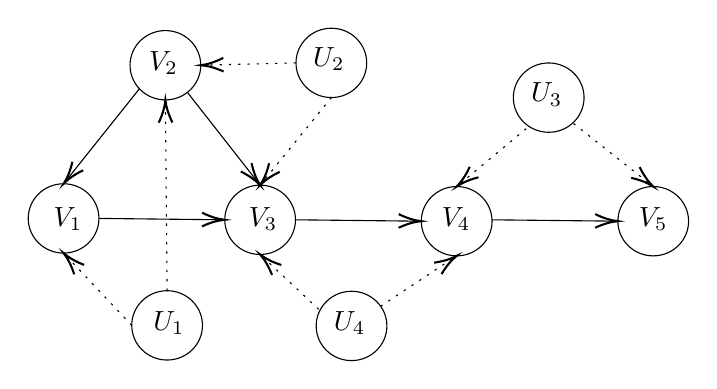
\begin{tikzpicture}[x=0.75pt,y=0.75pt,yscale=-1,xscale=1]
%uncomment if require: \path (0,249); %set diagram left start at 0, and has height of 249

%Straight Lines [id:da9409428103176911] 
\draw    (55.66,80.96) -- (20.28,125.27) ;
\draw [shift={(19.03,126.84)}, rotate = 308.61] [color={rgb, 255:red, 0; green, 0; blue, 0 }  ][line width=0.75]    (10.93,-3.29) .. controls (6.95,-1.4) and (3.31,-0.3) .. (0,0) .. controls (3.31,0.3) and (6.95,1.4) .. (10.93,3.29)   ;
%Shape: Ellipse [id:dp1957617230286519] 
\draw   (2,143.53) .. controls (2,134.31) and (9.63,126.84) .. (19.03,126.84) .. controls (28.44,126.84) and (36.06,134.31) .. (36.06,143.53) .. controls (36.06,152.76) and (28.44,160.23) .. (19.03,160.23) .. controls (9.63,160.23) and (2,152.76) .. (2,143.53) -- cycle ;
%Shape: Ellipse [id:dp3441414362261397] 
\draw   (96.7,144.2) .. controls (96.7,134.98) and (104.32,127.5) .. (113.73,127.5) .. controls (123.14,127.5) and (130.76,134.98) .. (130.76,144.2) .. controls (130.76,153.43) and (123.14,160.9) .. (113.73,160.9) .. controls (104.32,160.9) and (96.7,153.43) .. (96.7,144.2) -- cycle ;
%Shape: Ellipse [id:dp3332766589400997] 
\draw   (51.05,69.73) .. controls (51.05,60.51) and (58.68,53.03) .. (68.08,53.03) .. controls (77.49,53.03) and (85.12,60.51) .. (85.12,69.73) .. controls (85.12,78.95) and (77.49,86.43) .. (68.08,86.43) .. controls (58.68,86.43) and (51.05,78.95) .. (51.05,69.73) -- cycle ;
%Straight Lines [id:da23442985922821147] 
\draw    (36.06,143.53) -- (94.7,144.18) ;
\draw [shift={(96.7,144.2)}, rotate = 180.63] [color={rgb, 255:red, 0; green, 0; blue, 0 }  ][line width=0.75]    (10.93,-3.29) .. controls (6.95,-1.4) and (3.31,-0.3) .. (0,0) .. controls (3.31,0.3) and (6.95,1.4) .. (10.93,3.29)   ;
%Straight Lines [id:da30527808119318633] 
\draw    (78.82,82.97) -- (112.5,125.93) ;
\draw [shift={(113.73,127.5)}, rotate = 231.91] [color={rgb, 255:red, 0; green, 0; blue, 0 }  ][line width=0.75]    (10.93,-3.29) .. controls (6.95,-1.4) and (3.31,-0.3) .. (0,0) .. controls (3.31,0.3) and (6.95,1.4) .. (10.93,3.29)   ;
%Shape: Ellipse [id:dp4499667751102605] 
\draw   (191.39,144.87) .. controls (191.39,135.65) and (199.02,128.17) .. (208.43,128.17) .. controls (217.83,128.17) and (225.46,135.65) .. (225.46,144.87) .. controls (225.46,154.09) and (217.83,161.57) .. (208.43,161.57) .. controls (199.02,161.57) and (191.39,154.09) .. (191.39,144.87) -- cycle ;
%Straight Lines [id:da13037932973043498] 
\draw    (130.76,144.2) -- (189.4,144.85) ;
\draw [shift={(191.39,144.87)}, rotate = 180.63] [color={rgb, 255:red, 0; green, 0; blue, 0 }  ][line width=0.75]    (10.93,-3.29) .. controls (6.95,-1.4) and (3.31,-0.3) .. (0,0) .. controls (3.31,0.3) and (6.95,1.4) .. (10.93,3.29)   ;
%Shape: Ellipse [id:dp6469394084112792] 
\draw   (286.09,144.87) .. controls (286.09,135.65) and (293.72,128.17) .. (303.12,128.17) .. controls (312.53,128.17) and (320.16,135.65) .. (320.16,144.87) .. controls (320.16,154.09) and (312.53,161.57) .. (303.12,161.57) .. controls (293.72,161.57) and (286.09,154.09) .. (286.09,144.87) -- cycle ;
%Straight Lines [id:da27892547851212224] 
\draw    (225.46,144.2) -- (284.09,144.85) ;
\draw [shift={(286.09,144.87)}, rotate = 180.63] [color={rgb, 255:red, 0; green, 0; blue, 0 }  ][line width=0.75]    (10.93,-3.29) .. controls (6.95,-1.4) and (3.31,-0.3) .. (0,0) .. controls (3.31,0.3) and (6.95,1.4) .. (10.93,3.29)   ;
%Shape: Ellipse [id:dp35851974001279396] 
\draw   (51.88,195.06) .. controls (51.88,185.84) and (59.51,178.36) .. (68.92,178.36) .. controls (78.32,178.36) and (85.95,185.84) .. (85.95,195.06) .. controls (85.95,204.29) and (78.32,211.76) .. (68.92,211.76) .. controls (59.51,211.76) and (51.88,204.29) .. (51.88,195.06) -- cycle ;
%Straight Lines [id:da4145916339991944] 
\draw  [dash pattern={on 0.84pt off 2.51pt}]  (51.88,195.06) -- (20.4,161.69) ;
\draw [shift={(19.03,160.23)}, rotate = 46.67] [color={rgb, 255:red, 0; green, 0; blue, 0 }  ][line width=0.75]    (10.93,-3.29) .. controls (6.95,-1.4) and (3.31,-0.3) .. (0,0) .. controls (3.31,0.3) and (6.95,1.4) .. (10.93,3.29)   ;
%Straight Lines [id:da8882223061550982] 
\draw  [dash pattern={on 0.84pt off 2.51pt}]  (68.92,178.36) -- (68.1,88.43) ;
\draw [shift={(68.08,86.43)}, rotate = 89.48] [color={rgb, 255:red, 0; green, 0; blue, 0 }  ][line width=0.75]    (10.93,-3.29) .. controls (6.95,-1.4) and (3.31,-0.3) .. (0,0) .. controls (3.31,0.3) and (6.95,1.4) .. (10.93,3.29)   ;
%Shape: Ellipse [id:dp3160799529372307] 
\draw   (131.02,68.6) .. controls (131.02,59.38) and (138.64,51.9) .. (148.05,51.9) .. controls (157.46,51.9) and (165.08,59.38) .. (165.08,68.6) .. controls (165.08,77.83) and (157.46,85.3) .. (148.05,85.3) .. controls (138.64,85.3) and (131.02,77.83) .. (131.02,68.6) -- cycle ;
%Straight Lines [id:da5757039355297331] 
\draw  [dash pattern={on 0.84pt off 2.51pt}]  (148.05,85.3) -- (114.99,125.95) ;
\draw [shift={(113.73,127.5)}, rotate = 309.12] [color={rgb, 255:red, 0; green, 0; blue, 0 }  ][line width=0.75]    (10.93,-3.29) .. controls (6.95,-1.4) and (3.31,-0.3) .. (0,0) .. controls (3.31,0.3) and (6.95,1.4) .. (10.93,3.29)   ;
%Straight Lines [id:da8854762896558519] 
\draw  [dash pattern={on 0.84pt off 2.51pt}]  (131.02,68.6) -- (87.12,69.68) ;
\draw [shift={(85.12,69.73)}, rotate = 358.59] [color={rgb, 255:red, 0; green, 0; blue, 0 }  ][line width=0.75]    (10.93,-3.29) .. controls (6.95,-1.4) and (3.31,-0.3) .. (0,0) .. controls (3.31,0.3) and (6.95,1.4) .. (10.93,3.29)   ;
%Shape: Ellipse [id:dp730648475728567] 
\draw   (235.73,85.33) .. controls (235.73,76.11) and (243.36,68.63) .. (252.77,68.63) .. controls (262.17,68.63) and (269.8,76.11) .. (269.8,85.33) .. controls (269.8,94.56) and (262.17,102.03) .. (252.77,102.03) .. controls (243.36,102.03) and (235.73,94.56) .. (235.73,85.33) -- cycle ;
%Straight Lines [id:da11683998671197293] 
\draw  [dash pattern={on 0.84pt off 2.51pt}]  (264.76,97.85) -- (301.56,126.93) ;
\draw [shift={(303.12,128.17)}, rotate = 218.32] [color={rgb, 255:red, 0; green, 0; blue, 0 }  ][line width=0.75]    (10.93,-3.29) .. controls (6.95,-1.4) and (3.31,-0.3) .. (0,0) .. controls (3.31,0.3) and (6.95,1.4) .. (10.93,3.29)   ;
%Straight Lines [id:da3193898159682531] 
\draw  [dash pattern={on 0.84pt off 2.51pt}]  (241.93,100.3) -- (209.96,126.89) ;
\draw [shift={(208.43,128.17)}, rotate = 320.25] [color={rgb, 255:red, 0; green, 0; blue, 0 }  ][line width=0.75]    (10.93,-3.29) .. controls (6.95,-1.4) and (3.31,-0.3) .. (0,0) .. controls (3.31,0.3) and (6.95,1.4) .. (10.93,3.29)   ;
%Shape: Ellipse [id:dp41785845255033927] 
\draw   (140.73,195.33) .. controls (140.73,186.11) and (148.36,178.63) .. (157.77,178.63) .. controls (167.17,178.63) and (174.8,186.11) .. (174.8,195.33) .. controls (174.8,204.56) and (167.17,212.03) .. (157.77,212.03) .. controls (148.36,212.03) and (140.73,204.56) .. (140.73,195.33) -- cycle ;
%Straight Lines [id:da948110207954372] 
\draw  [dash pattern={on 0.84pt off 2.51pt}]  (171.76,185.85) -- (206.76,162.67) ;
\draw [shift={(208.43,161.57)}, rotate = 146.49] [color={rgb, 255:red, 0; green, 0; blue, 0 }  ][line width=0.75]    (10.93,-3.29) .. controls (6.95,-1.4) and (3.31,-0.3) .. (0,0) .. controls (3.31,0.3) and (6.95,1.4) .. (10.93,3.29)   ;
%Straight Lines [id:da6359994684445109] 
\draw  [dash pattern={on 0.84pt off 2.51pt}]  (141.93,187.3) -- (115.19,162.27) ;
\draw [shift={(113.73,160.9)}, rotate = 43.11] [color={rgb, 255:red, 0; green, 0; blue, 0 }  ][line width=0.75]    (10.93,-3.29) .. controls (6.95,-1.4) and (3.31,-0.3) .. (0,0) .. controls (3.31,0.3) and (6.95,1.4) .. (10.93,3.29)   ;


% Text Node
\draw (59,62) node [anchor=north west][inner sep=0.75pt]   [align=left] {$\displaystyle V_{2}$};
% Text Node
\draw (13,137) node [anchor=north west][inner sep=0.75pt]   [align=left] {$\displaystyle V_{1}$};
% Text Node
\draw (107,137) node [anchor=north west][inner sep=0.75pt]   [align=left] {$\displaystyle V_{3}$};
% Text Node
\draw (200,137) node [anchor=north west][inner sep=0.75pt]   [align=left] {$\displaystyle V_{4}{}$};
% Text Node
\draw (295,137) node [anchor=north west][inner sep=0.75pt]   [align=left] {$\displaystyle V_{5}{}$};
% Text Node
\draw (61,187) node [anchor=north west][inner sep=0.75pt]   [align=left] {$\displaystyle U_{1}{}$};
% Text Node
\draw (138,60) node [anchor=north west][inner sep=0.75pt]   [align=left] {$\displaystyle U_{2}{}$};
% Text Node
\draw (243,77) node [anchor=north west][inner sep=0.75pt]   [align=left] {$\displaystyle U_{3}{}$};
\draw (148,187) node [anchor=north west][inner sep=0.75pt]   [align=left] {$\displaystyle U_{4}{}$};
\end{tikzpicture}
}
\caption{An SCM example.}
\label{fig:scm_example}
\end{minipage}
\hfill
\begin{minipage}[t]{0.49\textwidth}
\resizebox{1\textwidth}{0.45\textwidth}{
\tikzset{every picture/.style={line width=0.75pt}} %set default line width to 0.75pt        

\tikzset{every picture/.style={line width=0.75pt}} %set default line width to 0.75pt        

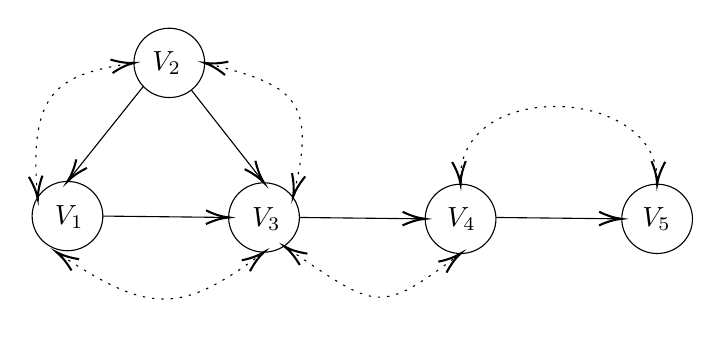
\begin{tikzpicture}[x=0.75pt,y=0.75pt,yscale=-1,xscale=1]
%uncomment if require: \path (0,249); %set diagram left start at 0, and has height of 249

%Straight Lines [id:da5670004967733733] 
\draw    (388.94,77.96) -- (353.57,122.27) ;
\draw [shift={(352.32,123.84)}, rotate = 308.61] [color={rgb, 255:red, 0; green, 0; blue, 0 }  ][line width=0.75]    (10.93,-3.29) .. controls (6.95,-1.4) and (3.31,-0.3) .. (0,0) .. controls (3.31,0.3) and (6.95,1.4) .. (10.93,3.29)   ;
%Shape: Ellipse [id:dp3687435720552046] 
\draw   (335.29,140.53) .. controls (335.29,131.31) and (342.91,123.84) .. (352.32,123.84) .. controls (361.73,123.84) and (369.35,131.31) .. (369.35,140.53) .. controls (369.35,149.76) and (361.73,157.23) .. (352.32,157.23) .. controls (342.91,157.23) and (335.29,149.76) .. (335.29,140.53) -- cycle ;
%Shape: Ellipse [id:dp37335162149277035] 
\draw   (429.98,141.2) .. controls (429.98,131.98) and (437.61,124.5) .. (447.02,124.5) .. controls (456.42,124.5) and (464.05,131.98) .. (464.05,141.2) .. controls (464.05,150.43) and (456.42,157.9) .. (447.02,157.9) .. controls (437.61,157.9) and (429.98,150.43) .. (429.98,141.2) -- cycle ;
%Shape: Ellipse [id:dp4171726010932877] 
\draw   (384.34,66.73) .. controls (384.34,57.51) and (391.96,50.03) .. (401.37,50.03) .. controls (410.78,50.03) and (418.4,57.51) .. (418.4,66.73) .. controls (418.4,75.95) and (410.78,83.43) .. (401.37,83.43) .. controls (391.96,83.43) and (384.34,75.95) .. (384.34,66.73) -- cycle ;
%Straight Lines [id:da13847113687899437] 
\draw    (369.35,140.53) -- (427.98,141.18) ;
\draw [shift={(429.98,141.2)}, rotate = 180.63] [color={rgb, 255:red, 0; green, 0; blue, 0 }  ][line width=0.75]    (10.93,-3.29) .. controls (6.95,-1.4) and (3.31,-0.3) .. (0,0) .. controls (3.31,0.3) and (6.95,1.4) .. (10.93,3.29)   ;
%Straight Lines [id:da42460288342391816] 
\draw    (412.11,79.97) -- (445.78,122.93) ;
\draw [shift={(447.02,124.5)}, rotate = 231.91] [color={rgb, 255:red, 0; green, 0; blue, 0 }  ][line width=0.75]    (10.93,-3.29) .. controls (6.95,-1.4) and (3.31,-0.3) .. (0,0) .. controls (3.31,0.3) and (6.95,1.4) .. (10.93,3.29)   ;
%Shape: Ellipse [id:dp2263302161318239] 
\draw   (524.68,141.87) .. controls (524.68,132.65) and (532.31,125.17) .. (541.71,125.17) .. controls (551.12,125.17) and (558.75,132.65) .. (558.75,141.87) .. controls (558.75,151.09) and (551.12,158.57) .. (541.71,158.57) .. controls (532.31,158.57) and (524.68,151.09) .. (524.68,141.87) -- cycle ;
%Straight Lines [id:da5872826292653424] 
\draw    (464.05,141.2) -- (522.68,141.85) ;
\draw [shift={(524.68,141.87)}, rotate = 180.63] [color={rgb, 255:red, 0; green, 0; blue, 0 }  ][line width=0.75]    (10.93,-3.29) .. controls (6.95,-1.4) and (3.31,-0.3) .. (0,0) .. controls (3.31,0.3) and (6.95,1.4) .. (10.93,3.29)   ;
%Shape: Ellipse [id:dp5861801177512753] 
\draw   (619.38,141.87) .. controls (619.38,132.65) and (627,125.17) .. (636.41,125.17) .. controls (645.82,125.17) and (653.44,132.65) .. (653.44,141.87) .. controls (653.44,151.09) and (645.82,158.57) .. (636.41,158.57) .. controls (627,158.57) and (619.38,151.09) .. (619.38,141.87) -- cycle ;
%Straight Lines [id:da2896517861834085] 
\draw    (558.75,141.2) -- (617.38,141.85) ;
\draw [shift={(619.38,141.87)}, rotate = 180.63] [color={rgb, 255:red, 0; green, 0; blue, 0 }  ][line width=0.75]    (10.93,-3.29) .. controls (6.95,-1.4) and (3.31,-0.3) .. (0,0) .. controls (3.31,0.3) and (6.95,1.4) .. (10.93,3.29)   ;
%Curve Lines [id:da8531288496156335] 
\draw  [dash pattern={on 0.84pt off 2.51pt}]  (349.02,159.25) .. controls (392.04,187.94) and (407.31,187.46) .. (445.84,158.78) ;
\draw [shift={(447.02,157.9)}, rotate = 143.13] [color={rgb, 255:red, 0; green, 0; blue, 0 }  ][line width=0.75]    (10.93,-3.29) .. controls (6.95,-1.4) and (3.31,-0.3) .. (0,0) .. controls (3.31,0.3) and (6.95,1.4) .. (10.93,3.29)   ;
\draw [shift={(347.02,157.9)}, rotate = 33.99] [color={rgb, 255:red, 0; green, 0; blue, 0 }  ][line width=0.75]    (10.93,-3.29) .. controls (6.95,-1.4) and (3.31,-0.3) .. (0,0) .. controls (3.31,0.3) and (6.95,1.4) .. (10.93,3.29)   ;
%Curve Lines [id:da9012300181854043] 
\draw  [dash pattern={on 0.84pt off 2.51pt}]  (461.54,129.12) .. controls (472.49,83.76) and (460.74,77.28) .. (420.27,67.19) ;
\draw [shift={(418.4,66.73)}, rotate = 13.87] [color={rgb, 255:red, 0; green, 0; blue, 0 }  ][line width=0.75]    (10.93,-3.29) .. controls (6.95,-1.4) and (3.31,-0.3) .. (0,0) .. controls (3.31,0.3) and (6.95,1.4) .. (10.93,3.29)   ;
\draw [shift={(461.02,131.25)}, rotate = 284.04] [color={rgb, 255:red, 0; green, 0; blue, 0 }  ][line width=0.75]    (10.93,-3.29) .. controls (6.95,-1.4) and (3.31,-0.3) .. (0,0) .. controls (3.31,0.3) and (6.95,1.4) .. (10.93,3.29)   ;
%Curve Lines [id:da7156302560368608] 
\draw  [dash pattern={on 0.84pt off 2.51pt}]  (382.19,67.06) .. controls (347.77,72.49) and (333.41,80.15) .. (337.88,130.71) ;
\draw [shift={(338.02,132.25)}, rotate = 264.61] [color={rgb, 255:red, 0; green, 0; blue, 0 }  ][line width=0.75]    (10.93,-3.29) .. controls (6.95,-1.4) and (3.31,-0.3) .. (0,0) .. controls (3.31,0.3) and (6.95,1.4) .. (10.93,3.29)   ;
\draw [shift={(384.34,66.73)}, rotate = 171.36] [color={rgb, 255:red, 0; green, 0; blue, 0 }  ][line width=0.75]    (10.93,-3.29) .. controls (6.95,-1.4) and (3.31,-0.3) .. (0,0) .. controls (3.31,0.3) and (6.95,1.4) .. (10.93,3.29)   ;
%Curve Lines [id:da5870313721281502] 
\draw  [dash pattern={on 0.84pt off 2.51pt}]  (636.46,123.04) .. controls (636.02,77.6) and (540.02,74.1) .. (541.63,123.65) ;
\draw [shift={(541.71,125.17)}, rotate = 265.93] [color={rgb, 255:red, 0; green, 0; blue, 0 }  ][line width=0.75]    (10.93,-3.29) .. controls (6.95,-1.4) and (3.31,-0.3) .. (0,0) .. controls (3.31,0.3) and (6.95,1.4) .. (10.93,3.29)   ;
\draw [shift={(636.41,125.17)}, rotate = 273.12] [color={rgb, 255:red, 0; green, 0; blue, 0 }  ][line width=0.75]    (10.93,-3.29) .. controls (6.95,-1.4) and (3.31,-0.3) .. (0,0) .. controls (3.31,0.3) and (6.95,1.4) .. (10.93,3.29)   ;
%Curve Lines [id:da41537558634390037] 
\draw  [dash pattern={on 0.84pt off 2.51pt}]  (459.01,156.6) .. controls (501.59,185.39) and (502.3,188.07) .. (540.54,159.45) ;
\draw [shift={(541.71,158.57)}, rotate = 143.13] [color={rgb, 255:red, 0; green, 0; blue, 0 }  ][line width=0.75]    (10.93,-3.29) .. controls (6.95,-1.4) and (3.31,-0.3) .. (0,0) .. controls (3.31,0.3) and (6.95,1.4) .. (10.93,3.29)   ;
\draw [shift={(457.02,155.25)}, rotate = 33.99] [color={rgb, 255:red, 0; green, 0; blue, 0 }  ][line width=0.75]    (10.93,-3.29) .. controls (6.95,-1.4) and (3.31,-0.3) .. (0,0) .. controls (3.31,0.3) and (6.95,1.4) .. (10.93,3.29)   ;

% Text Node
\draw (392,60) node [anchor=north west][inner sep=0.75pt]   [align=left] {$\displaystyle V_{2}$};
% Text Node
\draw (345,134) node [anchor=north west][inner sep=0.75pt]   [align=left] {$\displaystyle V_{1}$};
% Text Node
\draw (440,135) node [anchor=north west][inner sep=0.75pt]   [align=left] {$\displaystyle V_{3}$};
% Text Node
\draw (534,135) node [anchor=north west][inner sep=0.75pt]   [align=left] {$\displaystyle V_{4}{}$};
% Text Node
\draw (628,135) node [anchor=north west][inner sep=0.75pt]   [align=left] {$\displaystyle V_{5}{}$};
\end{tikzpicture}
}
\caption{The causal graph of this SCM. }
\label{fig:causal_graph}
\end{minipage}
\end{figure}
To further explain the notions in \cref{sec:preliminary}, we consider the following example. Let $\mathcal{M}$ be an SCM with the following structure equations.
\begin{align}
    &V_1 = f_1(V_2,U_1), \notag\\
    &V_2 = f_2(U_1,U_2), \notag\\
    &V_3 = f_3(V_1,V_2,U_2, U_4), \label{eq:se_example}\\
    &V_4 = f_4(V_3.U_3, U_4), \notag\\
    &V_5 = f_5(V_4,U_3), \notag
\end{align}
where $ U_1 $ and $U_2$ are correlated and $U_3,U_4$ and $(U_1,U_2)$ are independent. The causal model is shown in \cref{fig:scm_example} and its causal graph is shown in \cref{fig:causal_graph}.  In this example, $\boldsymbol{U}_{V_1} = \{U_1\},\boldsymbol{U}_{V_2} = \{U_1,U_2\},\boldsymbol{U}_{V_3} = \{U_2,U_4\}, \boldsymbol{U}_{V_4}= \{U_3,U_4\}, \boldsymbol{U}_{V_5} = \{U_3\}$. Since $U_1,U_2$ are correlated, $C_1 = \{ V_1,V_2,V_3 \}$ is one $C^2$ component because all nodes in $C_1$ are connected by bi-directed edges. Note that $\{V_1,V_2,V_3,V_4\}$ is not a $C^2$ component because $V_4$ and $V_2$ is not connected by any bi-directive edge. The rest of $C^2$ components are $C_2=\{V_4,V_5\}, C_3 = \{ V_3,V_4 \}$.\par 
Now, we consider the intervention $V_1 = t$. Under this intervention, the structure equations can be obtained by setting $V_1 = t$ while keeping all other equations unchanged, i.e., 
\begin{align*}
    &V_1(t) = t, \\
    &V_2(t) = f_2(U_1,U_2), \\
   &V_3 = f_3(V_1,V_2,U_2, U_4), \\
    &V_4 = f_4(V_3.U_3, U_4), \\
    &V_5(t) = f_5(V_4,U_3). \\
\end{align*}
The figure of this model under intervention is shown in \cref{fig:scm_example_int}. 
\begin{figure}[!htb]
    \centering



\tikzset{every picture/.style={line width=0.75pt}} %set default line width to 0.75pt        

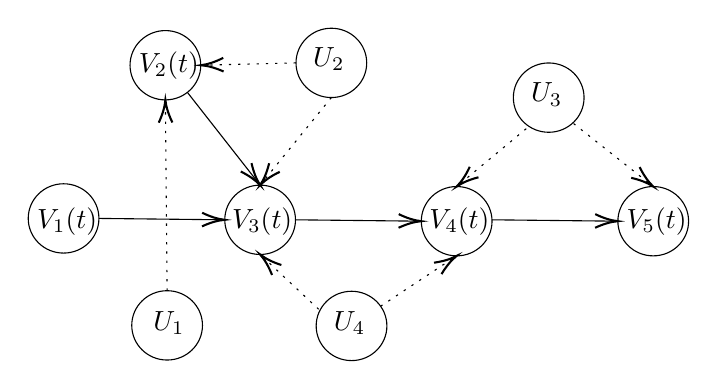
\begin{tikzpicture}[x=0.75pt,y=0.75pt,yscale=-1,xscale=1]
%uncomment if require: \path (0,249); %set diagram left start at 0, and has height of 249

%Straight Lines [id:da9409428103176911] 
%\draw    (55.66,80.96) -- (20.28,125.27) ;
%\draw [shift={(19.03,126.84)}, rotate = 308.61] [color={rgb, 255:red, 0; green, 0; blue, 0 }  ][line width=0.75]    (10.93,-3.29) .. controls (6.95,-1.4) and (3.31,-0.3) .. (0,0) .. controls (3.31,0.3) and (6.95,1.4) .. (10.93,3.29)   ;
%Shape: Ellipse [id:dp1957617230286519] 
\draw   (2,143.53) .. controls (2,134.31) and (9.63,126.84) .. (19.03,126.84) .. controls (28.44,126.84) and (36.06,134.31) .. (36.06,143.53) .. controls (36.06,152.76) and (28.44,160.23) .. (19.03,160.23) .. controls (9.63,160.23) and (2,152.76) .. (2,143.53) -- cycle ;
%Shape: Ellipse [id:dp3441414362261397] 
\draw   (96.7,144.2) .. controls (96.7,134.98) and (104.32,127.5) .. (113.73,127.5) .. controls (123.14,127.5) and (130.76,134.98) .. (130.76,144.2) .. controls (130.76,153.43) and (123.14,160.9) .. (113.73,160.9) .. controls (104.32,160.9) and (96.7,153.43) .. (96.7,144.2) -- cycle ;
%Shape: Ellipse [id:dp3332766589400997] 
\draw   (51.05,69.73) .. controls (51.05,60.51) and (58.68,53.03) .. (68.08,53.03) .. controls (77.49,53.03) and (85.12,60.51) .. (85.12,69.73) .. controls (85.12,78.95) and (77.49,86.43) .. (68.08,86.43) .. controls (58.68,86.43) and (51.05,78.95) .. (51.05,69.73) -- cycle ;
%Straight Lines [id:da23442985922821147] 
\draw    (36.06,143.53) -- (94.7,144.18) ;
\draw [shift={(96.7,144.2)}, rotate = 180.63] [color={rgb, 255:red, 0; green, 0; blue, 0 }  ][line width=0.75]    (10.93,-3.29) .. controls (6.95,-1.4) and (3.31,-0.3) .. (0,0) .. controls (3.31,0.3) and (6.95,1.4) .. (10.93,3.29)   ;
%Straight Lines [id:da30527808119318633] 
\draw    (78.82,82.97) -- (112.5,125.93) ;
\draw [shift={(113.73,127.5)}, rotate = 231.91] [color={rgb, 255:red, 0; green, 0; blue, 0 }  ][line width=0.75]    (10.93,-3.29) .. controls (6.95,-1.4) and (3.31,-0.3) .. (0,0) .. controls (3.31,0.3) and (6.95,1.4) .. (10.93,3.29)   ;
%Shape: Ellipse [id:dp4499667751102605] 
\draw   (191.39,144.87) .. controls (191.39,135.65) and (199.02,128.17) .. (208.43,128.17) .. controls (217.83,128.17) and (225.46,135.65) .. (225.46,144.87) .. controls (225.46,154.09) and (217.83,161.57) .. (208.43,161.57) .. controls (199.02,161.57) and (191.39,154.09) .. (191.39,144.87) -- cycle ;
%Straight Lines [id:da13037932973043498] 
\draw    (130.76,144.2) -- (189.4,144.85) ;
\draw [shift={(191.39,144.87)}, rotate = 180.63] [color={rgb, 255:red, 0; green, 0; blue, 0 }  ][line width=0.75]    (10.93,-3.29) .. controls (6.95,-1.4) and (3.31,-0.3) .. (0,0) .. controls (3.31,0.3) and (6.95,1.4) .. (10.93,3.29)   ;
%Shape: Ellipse [id:dp6469394084112792] 
\draw   (286.09,144.87) .. controls (286.09,135.65) and (293.72,128.17) .. (303.12,128.17) .. controls (312.53,128.17) and (320.16,135.65) .. (320.16,144.87) .. controls (320.16,154.09) and (312.53,161.57) .. (303.12,161.57) .. controls (293.72,161.57) and (286.09,154.09) .. (286.09,144.87) -- cycle ;
%Straight Lines [id:da27892547851212224] 
\draw    (225.46,144.2) -- (284.09,144.85) ;
\draw [shift={(286.09,144.87)}, rotate = 180.63] [color={rgb, 255:red, 0; green, 0; blue, 0 }  ][line width=0.75]    (10.93,-3.29) .. controls (6.95,-1.4) and (3.31,-0.3) .. (0,0) .. controls (3.31,0.3) and (6.95,1.4) .. (10.93,3.29)   ;
%Shape: Ellipse [id:dp35851974001279396] 
\draw   (51.88,195.06) .. controls (51.88,185.84) and (59.51,178.36) .. (68.92,178.36) .. controls (78.32,178.36) and (85.95,185.84) .. (85.95,195.06) .. controls (85.95,204.29) and (78.32,211.76) .. (68.92,211.76) .. controls (59.51,211.76) and (51.88,204.29) .. (51.88,195.06) -- cycle ;
%Straight Lines [id:da4145916339991944] 
%\draw  [dash pattern={on 0.84pt off 2.51pt}]  (51.88,195.06) -- (20.4,161.69) ;
%\draw [shift={(19.03,160.23)}, rotate = 46.67] [color={rgb, 255:red, 0; green, 0; blue, 0 }  ][line width=0.75]    (10.93,-3.29) .. controls (6.95,-1.4) and (3.31,-0.3) .. (0,0) .. controls (3.31,0.3) and (6.95,1.4) .. (10.93,3.29)   ;
%Straight Lines [id:da8882223061550982] 
\draw  [dash pattern={on 0.84pt off 2.51pt}]  (68.92,178.36) -- (68.1,88.43) ;
\draw [shift={(68.08,86.43)}, rotate = 89.48] [color={rgb, 255:red, 0; green, 0; blue, 0 }  ][line width=0.75]    (10.93,-3.29) .. controls (6.95,-1.4) and (3.31,-0.3) .. (0,0) .. controls (3.31,0.3) and (6.95,1.4) .. (10.93,3.29)   ;
%Shape: Ellipse [id:dp3160799529372307] 
\draw   (131.02,68.6) .. controls (131.02,59.38) and (138.64,51.9) .. (148.05,51.9) .. controls (157.46,51.9) and (165.08,59.38) .. (165.08,68.6) .. controls (165.08,77.83) and (157.46,85.3) .. (148.05,85.3) .. controls (138.64,85.3) and (131.02,77.83) .. (131.02,68.6) -- cycle ;
%Straight Lines [id:da5757039355297331] 
\draw  [dash pattern={on 0.84pt off 2.51pt}]  (148.05,85.3) -- (114.99,125.95) ;
\draw [shift={(113.73,127.5)}, rotate = 309.12] [color={rgb, 255:red, 0; green, 0; blue, 0 }  ][line width=0.75]    (10.93,-3.29) .. controls (6.95,-1.4) and (3.31,-0.3) .. (0,0) .. controls (3.31,0.3) and (6.95,1.4) .. (10.93,3.29)   ;
%Straight Lines [id:da8854762896558519] 
\draw  [dash pattern={on 0.84pt off 2.51pt}]  (131.02,68.6) -- (87.12,69.68) ;
\draw [shift={(85.12,69.73)}, rotate = 358.59] [color={rgb, 255:red, 0; green, 0; blue, 0 }  ][line width=0.75]    (10.93,-3.29) .. controls (6.95,-1.4) and (3.31,-0.3) .. (0,0) .. controls (3.31,0.3) and (6.95,1.4) .. (10.93,3.29)   ;
%Shape: Ellipse [id:dp730648475728567] 
\draw   (235.73,85.33) .. controls (235.73,76.11) and (243.36,68.63) .. (252.77,68.63) .. controls (262.17,68.63) and (269.8,76.11) .. (269.8,85.33) .. controls (269.8,94.56) and (262.17,102.03) .. (252.77,102.03) .. controls (243.36,102.03) and (235.73,94.56) .. (235.73,85.33) -- cycle ;
%Straight Lines [id:da11683998671197293] 
\draw  [dash pattern={on 0.84pt off 2.51pt}]  (264.76,97.85) -- (301.56,126.93) ;
\draw [shift={(303.12,128.17)}, rotate = 218.32] [color={rgb, 255:red, 0; green, 0; blue, 0 }  ][line width=0.75]    (10.93,-3.29) .. controls (6.95,-1.4) and (3.31,-0.3) .. (0,0) .. controls (3.31,0.3) and (6.95,1.4) .. (10.93,3.29)   ;
%Straight Lines [id:da3193898159682531] 
\draw  [dash pattern={on 0.84pt off 2.51pt}]  (241.93,100.3) -- (209.96,126.89) ;
\draw [shift={(208.43,128.17)}, rotate = 320.25] [color={rgb, 255:red, 0; green, 0; blue, 0 }  ][line width=0.75]    (10.93,-3.29) .. controls (6.95,-1.4) and (3.31,-0.3) .. (0,0) .. controls (3.31,0.3) and (6.95,1.4) .. (10.93,3.29)   ;
%Shape: Ellipse [id:dp41785845255033927] 
\draw   (140.73,195.33) .. controls (140.73,186.11) and (148.36,178.63) .. (157.77,178.63) .. controls (167.17,178.63) and (174.8,186.11) .. (174.8,195.33) .. controls (174.8,204.56) and (167.17,212.03) .. (157.77,212.03) .. controls (148.36,212.03) and (140.73,204.56) .. (140.73,195.33) -- cycle ;
%Straight Lines [id:da948110207954372] 
\draw  [dash pattern={on 0.84pt off 2.51pt}]  (171.76,185.85) -- (206.76,162.67) ;
\draw [shift={(208.43,161.57)}, rotate = 146.49] [color={rgb, 255:red, 0; green, 0; blue, 0 }  ][line width=0.75]    (10.93,-3.29) .. controls (6.95,-1.4) and (3.31,-0.3) .. (0,0) .. controls (3.31,0.3) and (6.95,1.4) .. (10.93,3.29)   ;
%Straight Lines [id:da6359994684445109] 
\draw  [dash pattern={on 0.84pt off 2.51pt}]  (141.93,187.3) -- (115.19,162.27) ;
\draw [shift={(113.73,160.9)}, rotate = 43.11] [color={rgb, 255:red, 0; green, 0; blue, 0 }  ][line width=0.75]    (10.93,-3.29) .. controls (6.95,-1.4) and (3.31,-0.3) .. (0,0) .. controls (3.31,0.3) and (6.95,1.4) .. (10.93,3.29)   ;


% Text Node
\draw (54,62) node [anchor=north west][inner sep=0.75pt]   [align=left] {$\displaystyle V_{2}(t)$};
% Text Node
\draw (5,137) node [anchor=north west][inner sep=0.75pt]   [align=left] {$\displaystyle V_{1}(t)$};
% Text Node
\draw (99,137) node [anchor=north west][inner sep=0.75pt]   [align=left] {$\displaystyle V_{3}(t)$};
% Text Node
\draw (194,137) node [anchor=north west][inner sep=0.75pt]   [align=left] {$\displaystyle V_{4}(t){}$};
% Text Node
\draw (289,137) node [anchor=north west][inner sep=0.75pt]   [align=left] {$\displaystyle V_{5}(t){}$};
% Text Node
\draw (61,187) node [anchor=north west][inner sep=0.75pt]   [align=left] {$\displaystyle U_{1}{}$};
% Text Node
\draw (138,60) node [anchor=north west][inner sep=0.75pt]   [align=left] {$\displaystyle U_{2}{}$};
% Text Node
\draw (243,77) node [anchor=north west][inner sep=0.75pt]   [align=left] {$\displaystyle U_{3}{}$};
\draw (148,187) node [anchor=north west][inner sep=0.75pt]   [align=left] {$\displaystyle U_{4}{}$};
\end{tikzpicture}
\caption{The SCM after intervention $V_1 = t$.}
\label{fig:scm_example_int}
\end{figure}

\iffalse
\section{Conclusion and Future Directions}
  In this paper, we provide theoretical justification for using NCMs for partial identification. We show that NCMs can be used to represent SCMs with complicated latent distributions under mild assumptions. The asymptotic consistency of the max/min estimator for partial identification is also proven. Besides, we take the first step to analyze the finite sample setting for the neural causal approach in a special setting. It remains unclear how to generalize the analysis to more general settings. In particular, a non-asymptotic analysis is still lacking. We leave this as a future research direction. 
\fi 

\section{Proof of approximation Theorems}

\subsection{Illustration of how to construct canonical representations and neural architectures}\label{sec:nn_example}
In this section, we illustrate how to construct canonical representations and neural architectures given a causal graph via a simple example. We consider the example in the previous section. The causal graph is shown in \cref{fig:causal_graph}. 

\begin{figure}[!htb]
    \centering
\begin{minipage}[t]{0.49\textwidth}
\resizebox{1\textwidth}{0.5\textwidth}{



\tikzset{every picture/.style={line width=0.75pt}} %set default line width to 0.75pt        

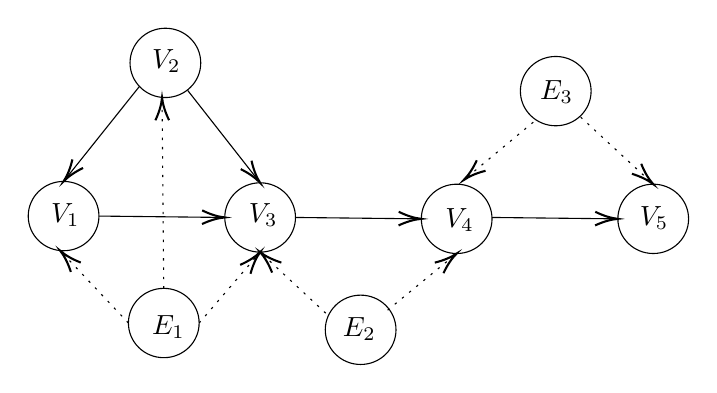
\begin{tikzpicture}[x=0.75pt,y=0.75pt,yscale=-1,xscale=1]
%uncomment if require: \path (0,300); %set diagram left start at 0, and has height of 300

%Straight Lines [id:da726236571308345] 
\draw    (68.27,45.96) -- (32.89,90.27) ;
\draw [shift={(31.64,91.84)}, rotate = 308.61] [color={rgb, 255:red, 0; green, 0; blue, 0 }  ][line width=0.75]    (10.93,-3.29) .. controls (6.95,-1.4) and (3.31,-0.3) .. (0,0) .. controls (3.31,0.3) and (6.95,1.4) .. (10.93,3.29)   ;
%Shape: Ellipse [id:dp9516912015591892] 
\draw   (14.61,108.53) .. controls (14.61,99.31) and (22.24,91.84) .. (31.64,91.84) .. controls (41.05,91.84) and (48.68,99.31) .. (48.68,108.53) .. controls (48.68,117.76) and (41.05,125.23) .. (31.64,125.23) .. controls (22.24,125.23) and (14.61,117.76) .. (14.61,108.53) -- cycle ;
%Shape: Ellipse [id:dp32485069026350377] 
\draw   (109.31,109.2) .. controls (109.31,99.98) and (116.93,92.5) .. (126.34,92.5) .. controls (135.75,92.5) and (143.37,99.98) .. (143.37,109.2) .. controls (143.37,118.43) and (135.75,125.9) .. (126.34,125.9) .. controls (116.93,125.9) and (109.31,118.43) .. (109.31,109.2) -- cycle ;
%Shape: Ellipse [id:dp17904550459729496] 
\draw   (63.66,34.73) .. controls (63.66,25.51) and (71.29,18.03) .. (80.7,18.03) .. controls (90.1,18.03) and (97.73,25.51) .. (97.73,34.73) .. controls (97.73,43.95) and (90.1,51.43) .. (80.7,51.43) .. controls (71.29,51.43) and (63.66,43.95) .. (63.66,34.73) -- cycle ;
%Straight Lines [id:da9211259582995228] 
\draw    (48.68,108.53) -- (107.31,109.18) ;
\draw [shift={(109.31,109.2)}, rotate = 180.63] [color={rgb, 255:red, 0; green, 0; blue, 0 }  ][line width=0.75]    (10.93,-3.29) .. controls (6.95,-1.4) and (3.31,-0.3) .. (0,0) .. controls (3.31,0.3) and (6.95,1.4) .. (10.93,3.29)   ;
%Straight Lines [id:da30495387690110975] 
\draw    (91.43,47.97) -- (125.11,90.93) ;
\draw [shift={(126.34,92.5)}, rotate = 231.91] [color={rgb, 255:red, 0; green, 0; blue, 0 }  ][line width=0.75]    (10.93,-3.29) .. controls (6.95,-1.4) and (3.31,-0.3) .. (0,0) .. controls (3.31,0.3) and (6.95,1.4) .. (10.93,3.29)   ;
%Shape: Ellipse [id:dp8984233439566385] 
\draw   (204.01,109.87) .. controls (204.01,100.65) and (211.63,93.17) .. (221.04,93.17) .. controls (230.45,93.17) and (238.07,100.65) .. (238.07,109.87) .. controls (238.07,119.09) and (230.45,126.57) .. (221.04,126.57) .. controls (211.63,126.57) and (204.01,119.09) .. (204.01,109.87) -- cycle ;
%Straight Lines [id:da8919326686442353] 
\draw    (143.37,109.2) -- (202.01,109.85) ;
\draw [shift={(204.01,109.87)}, rotate = 180.63] [color={rgb, 255:red, 0; green, 0; blue, 0 }  ][line width=0.75]    (10.93,-3.29) .. controls (6.95,-1.4) and (3.31,-0.3) .. (0,0) .. controls (3.31,0.3) and (6.95,1.4) .. (10.93,3.29)   ;
%Shape: Ellipse [id:dp7043084735647844] 
\draw   (298.7,109.87) .. controls (298.7,100.65) and (306.33,93.17) .. (315.74,93.17) .. controls (325.14,93.17) and (332.77,100.65) .. (332.77,109.87) .. controls (332.77,119.09) and (325.14,126.57) .. (315.74,126.57) .. controls (306.33,126.57) and (298.7,119.09) .. (298.7,109.87) -- cycle ;
%Straight Lines [id:da4176432168801385] 
\draw    (238.07,109.2) -- (296.7,109.85) ;
\draw [shift={(298.7,109.87)}, rotate = 180.63] [color={rgb, 255:red, 0; green, 0; blue, 0 }  ][line width=0.75]    (10.93,-3.29) .. controls (6.95,-1.4) and (3.31,-0.3) .. (0,0) .. controls (3.31,0.3) and (6.95,1.4) .. (10.93,3.29)   ;
%Shape: Ellipse [id:dp9233468195515437] 
\draw   (62.88,160.06) .. controls (62.88,150.84) and (70.51,143.36) .. (79.92,143.36) .. controls (89.32,143.36) and (96.95,150.84) .. (96.95,160.06) .. controls (96.95,169.29) and (89.32,176.76) .. (79.92,176.76) .. controls (70.51,176.76) and (62.88,169.29) .. (62.88,160.06) -- cycle ;
%Straight Lines [id:da06074623470934171] 
\draw  [dash pattern={on 0.84pt off 2.51pt}]  (62.88,160.06) -- (31.4,126.69) ;
\draw [shift={(30.03,125.23)}, rotate = 46.67] [color={rgb, 255:red, 0; green, 0; blue, 0 }  ][line width=0.75]    (10.93,-3.29) .. controls (6.95,-1.4) and (3.31,-0.3) .. (0,0) .. controls (3.31,0.3) and (6.95,1.4) .. (10.93,3.29)   ;
%Straight Lines [id:da32555516843150056] 
\draw  [dash pattern={on 0.84pt off 2.51pt}]  (79.92,143.36) -- (79.1,53.43) ;
\draw [shift={(79.08,51.43)}, rotate = 89.48] [color={rgb, 255:red, 0; green, 0; blue, 0 }  ][line width=0.75]    (10.93,-3.29) .. controls (6.95,-1.4) and (3.31,-0.3) .. (0,0) .. controls (3.31,0.3) and (6.95,1.4) .. (10.93,3.29)   ;
%Straight Lines [id:da7080275778580927] 
\draw  [dash pattern={on 0.84pt off 2.51pt}]  (96.95,160.06) -- (125.04,127.42) ;
\draw [shift={(126.34,125.9)}, rotate = 130.71] [color={rgb, 255:red, 0; green, 0; blue, 0 }  ][line width=0.75]    (10.93,-3.29) .. controls (6.95,-1.4) and (3.31,-0.3) .. (0,0) .. controls (3.31,0.3) and (6.95,1.4) .. (10.93,3.29)   ;
%Shape: Ellipse [id:dp19743884956016333] 
\draw   (157.73,163.33) .. controls (157.73,154.11) and (165.36,146.63) .. (174.77,146.63) .. controls (184.17,146.63) and (191.8,154.11) .. (191.8,163.33) .. controls (191.8,172.56) and (184.17,180.03) .. (174.77,180.03) .. controls (165.36,180.03) and (157.73,172.56) .. (157.73,163.33) -- cycle ;
%Straight Lines [id:da08874813939895398] 
\draw  [dash pattern={on 0.84pt off 2.51pt}]  (187.76,153.85) -- (219.49,127.84) ;
\draw [shift={(221.04,126.57)}, rotate = 140.66] [color={rgb, 255:red, 0; green, 0; blue, 0 }  ][line width=0.75]    (10.93,-3.29) .. controls (6.95,-1.4) and (3.31,-0.3) .. (0,0) .. controls (3.31,0.3) and (6.95,1.4) .. (10.93,3.29)   ;
%Straight Lines [id:da6947483522389868] 
\draw  [dash pattern={on 0.84pt off 2.51pt}]  (157.93,155.3) -- (127.81,127.26) ;
\draw [shift={(126.34,125.9)}, rotate = 42.95] [color={rgb, 255:red, 0; green, 0; blue, 0 }  ][line width=0.75]    (10.93,-3.29) .. controls (6.95,-1.4) and (3.31,-0.3) .. (0,0) .. controls (3.31,0.3) and (6.95,1.4) .. (10.93,3.29)   ;
%Shape: Ellipse [id:dp6890860962733356] 
\draw   (251.73,48.33) .. controls (251.73,39.11) and (259.36,31.63) .. (268.77,31.63) .. controls (278.17,31.63) and (285.8,39.11) .. (285.8,48.33) .. controls (285.8,57.56) and (278.17,65.03) .. (268.77,65.03) .. controls (259.36,65.03) and (251.73,57.56) .. (251.73,48.33) -- cycle ;
%Straight Lines [id:da060137045456188476] 
\draw  [dash pattern={on 0.84pt off 2.51pt}]  (280.76,60.85) -- (314.27,91.81) ;
\draw [shift={(315.74,93.17)}, rotate = 222.74] [color={rgb, 255:red, 0; green, 0; blue, 0 }  ][line width=0.75]    (10.93,-3.29) .. controls (6.95,-1.4) and (3.31,-0.3) .. (0,0) .. controls (3.31,0.3) and (6.95,1.4) .. (10.93,3.29)   ;
%Straight Lines [id:da2541333427878387] 
\draw  [dash pattern={on 0.84pt off 2.51pt}]  (257.93,63.3) -- (225.96,89.89) ;
\draw [shift={(224.43,91.17)}, rotate = 320.25] [color={rgb, 255:red, 0; green, 0; blue, 0 }  ][line width=0.75]    (10.93,-3.29) .. controls (6.95,-1.4) and (3.31,-0.3) .. (0,0) .. controls (3.31,0.3) and (6.95,1.4) .. (10.93,3.29)   ;

% Text Node
\draw (73.01,27.22) node [anchor=north west][inner sep=0.75pt]   [align=left] {$\displaystyle V_{2}$};
% Text Node
\draw (24.33,101.04) node [anchor=north west][inner sep=0.75pt]   [align=left] {$\displaystyle V_{1}$};
% Text Node
\draw (119.7,101.04) node [anchor=north west][inner sep=0.75pt]   [align=left] {$\displaystyle V_{3}$};
% Text Node
\draw (214.29,103.7) node [anchor=north west][inner sep=0.75pt]   [align=left] {$\displaystyle V_{4}{}$};
% Text Node
\draw (307.98,102.7) node [anchor=north west][inner sep=0.75pt]   [align=left] {$\displaystyle V_{5}{}$};
% Text Node
\draw (73,155) node [anchor=north west][inner sep=0.75pt]   [align=left] {$\displaystyle E_{1}{}$};
% Text Node
\draw (165,156) node [anchor=north west][inner sep=0.75pt]   [align=left] {$\displaystyle E_{2}{}$};
% Text Node
\draw (260,42) node [anchor=north west][inner sep=0.75pt]   [align=left] {$\displaystyle E_{3}{}$};


\end{tikzpicture}
}
\caption{The canonical representation of \cref{fig:causal_graph}.}
\label{fig:canoical}
\end{minipage}
\hfill
\begin{minipage}[t]{0.49\textwidth}
\resizebox{1\textwidth}{0.6\textwidth}{



\tikzset{every picture/.style={line width=0.75pt}} %set default line width to 0.75pt        

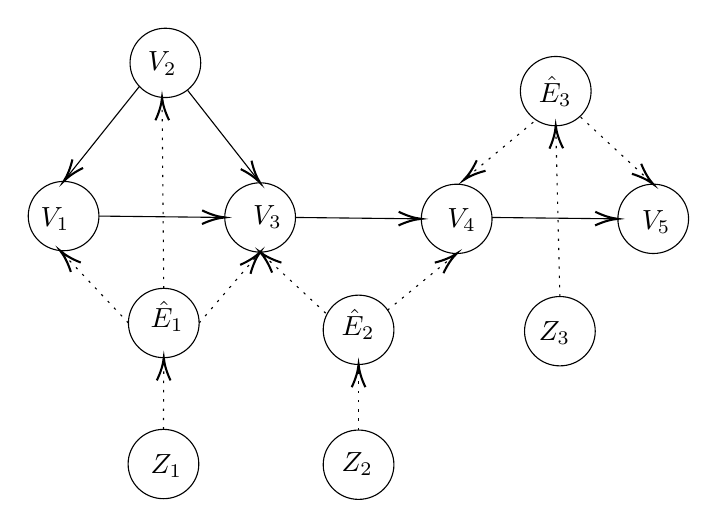
\begin{tikzpicture}[x=0.75pt,y=0.75pt,yscale=-1,xscale=1]
%uncomment if require: \path (0,300); %set diagram left start at 0, and has height of 300

%Straight Lines [id:da3296260132287745] 
\draw    (396.94,95.96) -- (361.57,140.27) ;
\draw [shift={(360.32,141.84)}, rotate = 308.61] [color={rgb, 255:red, 0; green, 0; blue, 0 }  ][line width=0.75]    (10.93,-3.29) .. controls (6.95,-1.4) and (3.31,-0.3) .. (0,0) .. controls (3.31,0.3) and (6.95,1.4) .. (10.93,3.29)   ;
%Shape: Ellipse [id:dp1163381972460964] 
\draw   (343.29,158.53) .. controls (343.29,149.31) and (350.91,141.84) .. (360.32,141.84) .. controls (369.73,141.84) and (377.35,149.31) .. (377.35,158.53) .. controls (377.35,167.76) and (369.73,175.23) .. (360.32,175.23) .. controls (350.91,175.23) and (343.29,167.76) .. (343.29,158.53) -- cycle ;
%Shape: Ellipse [id:dp394856712197859] 
\draw   (437.98,159.2) .. controls (437.98,149.98) and (445.61,142.5) .. (455.02,142.5) .. controls (464.42,142.5) and (472.05,149.98) .. (472.05,159.2) .. controls (472.05,168.43) and (464.42,175.9) .. (455.02,175.9) .. controls (445.61,175.9) and (437.98,168.43) .. (437.98,159.2) -- cycle ;
%Shape: Ellipse [id:dp9406190552132767] 
\draw   (392.34,84.73) .. controls (392.34,75.51) and (399.96,68.03) .. (409.37,68.03) .. controls (418.78,68.03) and (426.4,75.51) .. (426.4,84.73) .. controls (426.4,93.95) and (418.78,101.43) .. (409.37,101.43) .. controls (399.96,101.43) and (392.34,93.95) .. (392.34,84.73) -- cycle ;
%Straight Lines [id:da2546913423175581] 
\draw    (377.35,158.53) -- (435.98,159.18) ;
\draw [shift={(437.98,159.2)}, rotate = 180.63] [color={rgb, 255:red, 0; green, 0; blue, 0 }  ][line width=0.75]    (10.93,-3.29) .. controls (6.95,-1.4) and (3.31,-0.3) .. (0,0) .. controls (3.31,0.3) and (6.95,1.4) .. (10.93,3.29)   ;
%Straight Lines [id:da42382310214618646] 
\draw    (420.11,97.97) -- (453.78,140.93) ;
\draw [shift={(455.02,142.5)}, rotate = 231.91] [color={rgb, 255:red, 0; green, 0; blue, 0 }  ][line width=0.75]    (10.93,-3.29) .. controls (6.95,-1.4) and (3.31,-0.3) .. (0,0) .. controls (3.31,0.3) and (6.95,1.4) .. (10.93,3.29)   ;
%Shape: Ellipse [id:dp8517416675012104] 
\draw   (532.68,159.87) .. controls (532.68,150.65) and (540.31,143.17) .. (549.71,143.17) .. controls (559.12,143.17) and (566.75,150.65) .. (566.75,159.87) .. controls (566.75,169.09) and (559.12,176.57) .. (549.71,176.57) .. controls (540.31,176.57) and (532.68,169.09) .. (532.68,159.87) -- cycle ;
%Straight Lines [id:da7167276148961388] 
\draw    (472.05,159.2) -- (530.68,159.85) ;
\draw [shift={(532.68,159.87)}, rotate = 180.63] [color={rgb, 255:red, 0; green, 0; blue, 0 }  ][line width=0.75]    (10.93,-3.29) .. controls (6.95,-1.4) and (3.31,-0.3) .. (0,0) .. controls (3.31,0.3) and (6.95,1.4) .. (10.93,3.29)   ;
%Shape: Ellipse [id:dp6049197873452994] 
\draw   (627.38,159.87) .. controls (627.38,150.65) and (635,143.17) .. (644.41,143.17) .. controls (653.82,143.17) and (661.44,150.65) .. (661.44,159.87) .. controls (661.44,169.09) and (653.82,176.57) .. (644.41,176.57) .. controls (635,176.57) and (627.38,169.09) .. (627.38,159.87) -- cycle ;
%Straight Lines [id:da06879618588531411] 
\draw    (566.75,159.2) -- (625.38,159.85) ;
\draw [shift={(627.38,159.87)}, rotate = 180.63] [color={rgb, 255:red, 0; green, 0; blue, 0 }  ][line width=0.75]    (10.93,-3.29) .. controls (6.95,-1.4) and (3.31,-0.3) .. (0,0) .. controls (3.31,0.3) and (6.95,1.4) .. (10.93,3.29)   ;
%Shape: Ellipse [id:dp03656035760085663] 
\draw   (391.56,210.06) .. controls (391.56,200.84) and (399.18,193.36) .. (408.59,193.36) .. controls (418,193.36) and (425.62,200.84) .. (425.62,210.06) .. controls (425.62,219.29) and (418,226.76) .. (408.59,226.76) .. controls (399.18,226.76) and (391.56,219.29) .. (391.56,210.06) -- cycle ;
%Straight Lines [id:da14658442012688067] 
\draw  [dash pattern={on 0.84pt off 2.51pt}]  (391.56,210.06) -- (360.08,176.69) ;
\draw [shift={(358.71,175.23)}, rotate = 46.67] [color={rgb, 255:red, 0; green, 0; blue, 0 }  ][line width=0.75]    (10.93,-3.29) .. controls (6.95,-1.4) and (3.31,-0.3) .. (0,0) .. controls (3.31,0.3) and (6.95,1.4) .. (10.93,3.29)   ;
%Straight Lines [id:da23649264141628534] 
\draw  [dash pattern={on 0.84pt off 2.51pt}]  (408.59,193.36) -- (407.78,103.43) ;
\draw [shift={(407.76,101.43)}, rotate = 89.48] [color={rgb, 255:red, 0; green, 0; blue, 0 }  ][line width=0.75]    (10.93,-3.29) .. controls (6.95,-1.4) and (3.31,-0.3) .. (0,0) .. controls (3.31,0.3) and (6.95,1.4) .. (10.93,3.29)   ;
%Straight Lines [id:da7208531655007815] 
\draw  [dash pattern={on 0.84pt off 2.51pt}]  (425.62,210.06) -- (453.71,177.42) ;
\draw [shift={(455.02,175.9)}, rotate = 130.71] [color={rgb, 255:red, 0; green, 0; blue, 0 }  ][line width=0.75]    (10.93,-3.29) .. controls (6.95,-1.4) and (3.31,-0.3) .. (0,0) .. controls (3.31,0.3) and (6.95,1.4) .. (10.93,3.29)   ;
%Shape: Ellipse [id:dp6558416056912153] 
\draw   (485.41,213.33) .. controls (485.41,204.11) and (493.03,196.63) .. (502.44,196.63) .. controls (511.85,196.63) and (519.47,204.11) .. (519.47,213.33) .. controls (519.47,222.56) and (511.85,230.03) .. (502.44,230.03) .. controls (493.03,230.03) and (485.41,222.56) .. (485.41,213.33) -- cycle ;
%Straight Lines [id:da6989266488239831] 
\draw  [dash pattern={on 0.84pt off 2.51pt}]  (516.43,203.85) -- (548.17,177.84) ;
\draw [shift={(549.71,176.57)}, rotate = 140.66] [color={rgb, 255:red, 0; green, 0; blue, 0 }  ][line width=0.75]    (10.93,-3.29) .. controls (6.95,-1.4) and (3.31,-0.3) .. (0,0) .. controls (3.31,0.3) and (6.95,1.4) .. (10.93,3.29)   ;
%Straight Lines [id:da5586055042388729] 
\draw  [dash pattern={on 0.84pt off 2.51pt}]  (486.6,205.3) -- (456.48,177.26) ;
\draw [shift={(455.02,175.9)}, rotate = 42.95] [color={rgb, 255:red, 0; green, 0; blue, 0 }  ][line width=0.75]    (10.93,-3.29) .. controls (6.95,-1.4) and (3.31,-0.3) .. (0,0) .. controls (3.31,0.3) and (6.95,1.4) .. (10.93,3.29)   ;
%Shape: Ellipse [id:dp7886297647194405] 
\draw   (580.41,98.33) .. controls (580.41,89.11) and (588.03,81.63) .. (597.44,81.63) .. controls (606.85,81.63) and (614.47,89.11) .. (614.47,98.33) .. controls (614.47,107.56) and (606.85,115.03) .. (597.44,115.03) .. controls (588.03,115.03) and (580.41,107.56) .. (580.41,98.33) -- cycle ;
%Straight Lines [id:da6416033369666276] 
\draw  [dash pattern={on 0.84pt off 2.51pt}]  (609.43,110.85) -- (642.94,141.81) ;
\draw [shift={(644.41,143.17)}, rotate = 222.74] [color={rgb, 255:red, 0; green, 0; blue, 0 }  ][line width=0.75]    (10.93,-3.29) .. controls (6.95,-1.4) and (3.31,-0.3) .. (0,0) .. controls (3.31,0.3) and (6.95,1.4) .. (10.93,3.29)   ;
%Straight Lines [id:da9323123111672502] 
\draw  [dash pattern={on 0.84pt off 2.51pt}]  (586.6,113.3) -- (554.64,139.89) ;
\draw [shift={(553.1,141.17)}, rotate = 320.25] [color={rgb, 255:red, 0; green, 0; blue, 0 }  ][line width=0.75]    (10.93,-3.29) .. controls (6.95,-1.4) and (3.31,-0.3) .. (0,0) .. controls (3.31,0.3) and (6.95,1.4) .. (10.93,3.29)   ;
%Shape: Ellipse [id:dp4181999025328682] 
\draw   (485.41,278.33) .. controls (485.41,269.11) and (493.03,261.63) .. (502.44,261.63) .. controls (511.85,261.63) and (519.47,269.11) .. (519.47,278.33) .. controls (519.47,287.56) and (511.85,295.03) .. (502.44,295.03) .. controls (493.03,295.03) and (485.41,287.56) .. (485.41,278.33) -- cycle ;
%Shape: Ellipse [id:dp014471196165171785] 
\draw   (391.41,278) .. controls (391.41,268.78) and (399.03,261.3) .. (408.44,261.3) .. controls (417.85,261.3) and (425.47,268.78) .. (425.47,278) .. controls (425.47,287.23) and (417.85,294.7) .. (408.44,294.7) .. controls (399.03,294.7) and (391.41,287.23) .. (391.41,278) -- cycle ;
%Straight Lines [id:da08923180180283374] 
\draw  [dash pattern={on 0.84pt off 2.51pt}]  (408.44,261.3) -- (408.58,228.76) ;
\draw [shift={(408.59,226.76)}, rotate = 90.25] [color={rgb, 255:red, 0; green, 0; blue, 0 }  ][line width=0.75]    (10.93,-3.29) .. controls (6.95,-1.4) and (3.31,-0.3) .. (0,0) .. controls (3.31,0.3) and (6.95,1.4) .. (10.93,3.29)   ;
%Straight Lines [id:da9281674759459277] 
\draw  [dash pattern={on 0.84pt off 2.51pt}]  (502.44,261.63) -- (502.44,232.03) ;
\draw [shift={(502.44,230.03)}, rotate = 90] [color={rgb, 255:red, 0; green, 0; blue, 0 }  ][line width=0.75]    (10.93,-3.29) .. controls (6.95,-1.4) and (3.31,-0.3) .. (0,0) .. controls (3.31,0.3) and (6.95,1.4) .. (10.93,3.29)   ;
%Shape: Ellipse [id:dp9482638545383453] 
\draw   (582.41,214) .. controls (582.41,204.78) and (590.03,197.3) .. (599.44,197.3) .. controls (608.85,197.3) and (616.47,204.78) .. (616.47,214) .. controls (616.47,223.23) and (608.85,230.7) .. (599.44,230.7) .. controls (590.03,230.7) and (582.41,223.23) .. (582.41,214) -- cycle ;
%Straight Lines [id:da24357805593279336] 
\draw  [dash pattern={on 0.84pt off 2.51pt}]  (599.44,197.3) -- (597.49,117.03) ;
\draw [shift={(597.44,115.03)}, rotate = 88.61] [color={rgb, 255:red, 0; green, 0; blue, 0 }  ][line width=0.75]    (10.93,-3.29) .. controls (6.95,-1.4) and (3.31,-0.3) .. (0,0) .. controls (3.31,0.3) and (6.95,1.4) .. (10.93,3.29)   ;

% Text Node
\draw (399.69,78.22) node [anchor=north west][inner sep=0.75pt]   [align=left] {$\displaystyle V_{2}$};
% Text Node
\draw (348,153.04) node [anchor=north west][inner sep=0.75pt]   [align=left] {$\displaystyle V_{1}$};
% Text Node
\draw (450.38,152.04) node [anchor=north west][inner sep=0.75pt]   [align=left] {$\displaystyle V_{3}$};
% Text Node
\draw (543.96,153.7) node [anchor=north west][inner sep=0.75pt]   [align=left] {$\displaystyle V_{4}{}$};
% Text Node
\draw (637.66,154.7) node [anchor=north west][inner sep=0.75pt]   [align=left] {$\displaystyle V_{5}{}$};
% Text Node
\draw (400.99,198.41) node [anchor=north west][inner sep=0.75pt]   [align=left] {$\displaystyle \hat{E}_{1}{}$};
% Text Node
\draw (493,202) node [anchor=north west][inner sep=0.75pt]   [align=left] {$\displaystyle \hat{E}_{2}{}$};
% Text Node
\draw (588,90) node [anchor=north west][inner sep=0.75pt]   [align=left] {$\displaystyle \hat{E}_{3}{}$};
% Text Node
\draw (493,271.33) node [anchor=north west][inner sep=0.75pt]   [align=left] {$\displaystyle Z_{2}$};
% Text Node
\draw (400.99,272) node [anchor=north west][inner sep=0.75pt]   [align=left] {$\displaystyle Z_{1}$};
% Text Node
\draw (588,208) node [anchor=north west][inner sep=0.75pt]   [align=left] {$\displaystyle Z_{3}$};


\end{tikzpicture}

}
\caption{The neural network architecture.}
\label{fig:architecture}
\end{minipage}
\end{figure}

Following the construction in \cref{prop:equivalent_g_constrianed}, we use one latent variable for each $C^2$ component. As we explain in \cref{sec:illus_scm}, this causal model has three $C^2$ components, $ \{V_1,V_2,V_3\}, \{V_3,V_4\}, \{V_4,V_5\} $. In the canonical representation, exactly the latent variables enter their corresponding $C^2$ component. The structure equation of this SCM is as follows. 
\begin{align}
    &V_1 = f_1(V_2,E_1), \notag\\
    &V_2 = f_2(E_1), \notag\\
    &V_3 = f_3(V_1,V_2,E_1,E_2), \label{eq:se_canonical}\\
    &V_4 = f_4(V_3.E_2), \notag\\
    &V_5 = f_5(V_4,E_3), \notag
\end{align}
If we set $E_1 = (U_1,U_2), E_2 = U_4, E_3 = U_3$, (\ref{eq:se_canonical}) is equivalent to (\ref{eq:se_example}). Therefore, we can see from this example that the canonical representation does not lose any information about the SCM. 

Now, we show how to construct the NCM architecture from a canonical representation. As we mentioned in Section 3, we approximate the latent distribution by pushing forward uniform and Gumbel variables. The structure equation of the NCM is 
\begin{align}
    &V_1 = f^{\theta_1}_1(V_2,g_1^{\theta_1}(Z_1)), \notag\\
    &V_2 = f^{\theta_2}_2(g_1^{\theta_1}(Z_1)), \notag\\
    &V_3 = f^{\theta_2}_3(V_1,V_2,g_1^{\theta_1}(Z_1),g_2^{\theta_1}(Z_2)), \label{eq:se_canonical2}\\
    &V_4 = f_4^{\theta_4}(V_3.g_2^{\theta_1}(Z_2)), \notag\\
    &V_5 = f_5^{\theta_5}(V_4,g_2^{\theta_3}(Z_3)), \notag
\end{align}
where $f_i^{\theta_i}, g_j^{\theta_j}$ are neural networks, $Z_i$ are join distribution of independent uniform and Gumbel variables, and $g_j^{\theta_j}$ has the special architecture described in Section 3.1 and Section 3.2. \cref{fig:architecture} shows the architecture of the NCM. Each in-edge represents an input of a neural net.  

\subsection{Proof of \cref{thm:approximation}}
The causal graph $ \mathcal{G} $ does not specify how latent variables influence the observed variables. There could be many ways of recovering the latent variables from a graph $\mathcal{G}$. \cref{fig:example} shows an example where two different causal models have the same causal graph. The next proposition gives a canonical representation of a causal model. 
\begin{figure}[!htb]
  \centering
  



\tikzset{every picture/.style={line width=0.75pt}} %set default line width to 0.75pt        

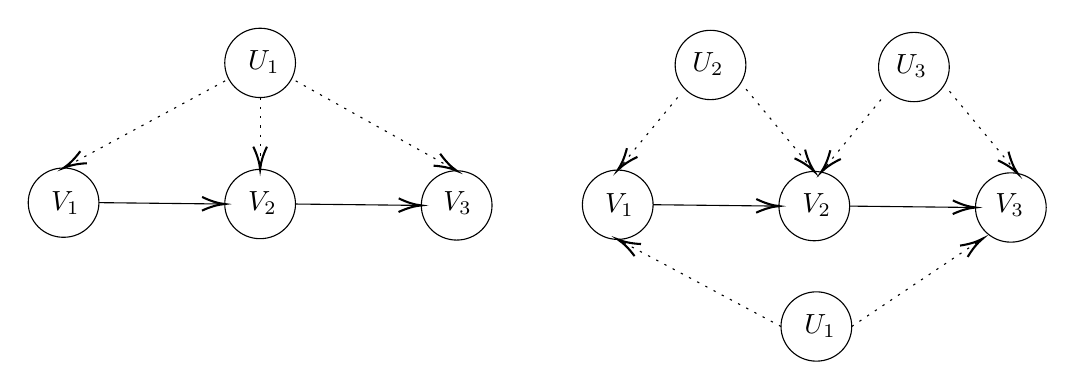
\begin{tikzpicture}[x=0.75pt,y=0.75pt,yscale=-1,xscale=1]
%uncomment if require: \path (0,300); %set diagram left start at 0, and has height of 300

%Shape: Ellipse [id:dp1974594692304923] 
\draw   (35.29,163.53) .. controls (35.29,154.31) and (42.91,146.84) .. (52.32,146.84) .. controls (61.73,146.84) and (69.35,154.31) .. (69.35,163.53) .. controls (69.35,172.76) and (61.73,180.23) .. (52.32,180.23) .. controls (42.91,180.23) and (35.29,172.76) .. (35.29,163.53) -- cycle ;
%Shape: Ellipse [id:dp48208910323030474] 
\draw   (129.98,164.2) .. controls (129.98,154.98) and (137.61,147.5) .. (147.02,147.5) .. controls (156.42,147.5) and (164.05,154.98) .. (164.05,164.2) .. controls (164.05,173.43) and (156.42,180.9) .. (147.02,180.9) .. controls (137.61,180.9) and (129.98,173.43) .. (129.98,164.2) -- cycle ;
%Straight Lines [id:da7962005744728682] 
\draw    (69.35,163.53) -- (127.98,164.18) ;
\draw [shift={(129.98,164.2)}, rotate = 180.63] [color={rgb, 255:red, 0; green, 0; blue, 0 }  ][line width=0.75]    (10.93,-3.29) .. controls (6.95,-1.4) and (3.31,-0.3) .. (0,0) .. controls (3.31,0.3) and (6.95,1.4) .. (10.93,3.29)   ;
%Shape: Ellipse [id:dp4908642218314525] 
\draw   (224.68,164.87) .. controls (224.68,155.65) and (232.31,148.17) .. (241.71,148.17) .. controls (251.12,148.17) and (258.75,155.65) .. (258.75,164.87) .. controls (258.75,174.09) and (251.12,181.57) .. (241.71,181.57) .. controls (232.31,181.57) and (224.68,174.09) .. (224.68,164.87) -- cycle ;
%Straight Lines [id:da6721782600602264] 
\draw    (164.05,164.2) -- (222.68,164.85) ;
\draw [shift={(224.68,164.87)}, rotate = 180.63] [color={rgb, 255:red, 0; green, 0; blue, 0 }  ][line width=0.75]    (10.93,-3.29) .. controls (6.95,-1.4) and (3.31,-0.3) .. (0,0) .. controls (3.31,0.3) and (6.95,1.4) .. (10.93,3.29)   ;
%Straight Lines [id:da8601815219575197] 
\draw  [dash pattern={on 0.84pt off 2.51pt}]  (147.02,112.9) -- (147.02,145.5) ;
\draw [shift={(147.02,147.5)}, rotate = 270] [color={rgb, 255:red, 0; green, 0; blue, 0 }  ][line width=0.75]    (10.93,-3.29) .. controls (6.95,-1.4) and (3.31,-0.3) .. (0,0) .. controls (3.31,0.3) and (6.95,1.4) .. (10.93,3.29)   ;
%Straight Lines [id:da5039443878791565] 
\draw  [dash pattern={on 0.84pt off 2.51pt}]  (164.16,104.87) -- (239.97,147.2) ;
\draw [shift={(241.71,148.17)}, rotate = 209.17] [color={rgb, 255:red, 0; green, 0; blue, 0 }  ][line width=0.75]    (10.93,-3.29) .. controls (6.95,-1.4) and (3.31,-0.3) .. (0,0) .. controls (3.31,0.3) and (6.95,1.4) .. (10.93,3.29)   ;
%Shape: Ellipse [id:dp815110305963826] 
\draw   (129.98,96.2) .. controls (129.98,86.98) and (137.61,79.5) .. (147.02,79.5) .. controls (156.42,79.5) and (164.05,86.98) .. (164.05,96.2) .. controls (164.05,105.43) and (156.42,112.9) .. (147.02,112.9) .. controls (137.61,112.9) and (129.98,105.43) .. (129.98,96.2) -- cycle ;
%Straight Lines [id:da9281104527151505] 
\draw  [dash pattern={on 0.84pt off 2.51pt}]  (130.16,104.87) -- (54.08,145.89) ;
\draw [shift={(52.32,146.84)}, rotate = 331.67] [color={rgb, 255:red, 0; green, 0; blue, 0 }  ][line width=0.75]    (10.93,-3.29) .. controls (6.95,-1.4) and (3.31,-0.3) .. (0,0) .. controls (3.31,0.3) and (6.95,1.4) .. (10.93,3.29)   ;
%Shape: Ellipse [id:dp14946237102463122] 
\draw   (302.29,164.53) .. controls (302.29,155.31) and (309.91,147.84) .. (319.32,147.84) .. controls (328.73,147.84) and (336.35,155.31) .. (336.35,164.53) .. controls (336.35,173.76) and (328.73,181.23) .. (319.32,181.23) .. controls (309.91,181.23) and (302.29,173.76) .. (302.29,164.53) -- cycle ;
%Shape: Ellipse [id:dp6206761464354984] 
\draw   (396.98,165.2) .. controls (396.98,155.98) and (404.61,148.5) .. (414.02,148.5) .. controls (423.42,148.5) and (431.05,155.98) .. (431.05,165.2) .. controls (431.05,174.43) and (423.42,181.9) .. (414.02,181.9) .. controls (404.61,181.9) and (396.98,174.43) .. (396.98,165.2) -- cycle ;
%Straight Lines [id:da9755966967921046] 
\draw    (336.35,164.53) -- (394.98,165.18) ;
\draw [shift={(396.98,165.2)}, rotate = 180.63] [color={rgb, 255:red, 0; green, 0; blue, 0 }  ][line width=0.75]    (10.93,-3.29) .. controls (6.95,-1.4) and (3.31,-0.3) .. (0,0) .. controls (3.31,0.3) and (6.95,1.4) .. (10.93,3.29)   ;
%Shape: Ellipse [id:dp04593532388079913] 
\draw   (491.68,165.87) .. controls (491.68,156.65) and (499.31,149.17) .. (508.71,149.17) .. controls (518.12,149.17) and (525.75,156.65) .. (525.75,165.87) .. controls (525.75,175.09) and (518.12,182.57) .. (508.71,182.57) .. controls (499.31,182.57) and (491.68,175.09) .. (491.68,165.87) -- cycle ;
%Straight Lines [id:da3548748087409026] 
\draw    (431.05,165.2) -- (489.68,165.85) ;
\draw [shift={(491.68,165.87)}, rotate = 180.63] [color={rgb, 255:red, 0; green, 0; blue, 0 }  ][line width=0.75]    (10.93,-3.29) .. controls (6.95,-1.4) and (3.31,-0.3) .. (0,0) .. controls (3.31,0.3) and (6.95,1.4) .. (10.93,3.29)   ;
%Straight Lines [id:da6133126970842009] 
\draw  [dash pattern={on 0.84pt off 2.51pt}]  (381.16,108.87) -- (412.74,146.96) ;
\draw [shift={(414.02,148.5)}, rotate = 230.34] [color={rgb, 255:red, 0; green, 0; blue, 0 }  ][line width=0.75]    (10.93,-3.29) .. controls (6.95,-1.4) and (3.31,-0.3) .. (0,0) .. controls (3.31,0.3) and (6.95,1.4) .. (10.93,3.29)   ;
%Shape: Ellipse [id:dp6926096369638808] 
\draw   (346.98,97.2) .. controls (346.98,87.98) and (354.61,80.5) .. (364.02,80.5) .. controls (373.42,80.5) and (381.05,87.98) .. (381.05,97.2) .. controls (381.05,106.43) and (373.42,113.9) .. (364.02,113.9) .. controls (354.61,113.9) and (346.98,106.43) .. (346.98,97.2) -- cycle ;
%Straight Lines [id:da5376861884507544] 
\draw  [dash pattern={on 0.84pt off 2.51pt}]  (348.16,112.87) -- (320.59,146.29) ;
\draw [shift={(319.32,147.84)}, rotate = 309.52] [color={rgb, 255:red, 0; green, 0; blue, 0 }  ][line width=0.75]    (10.93,-3.29) .. controls (6.95,-1.4) and (3.31,-0.3) .. (0,0) .. controls (3.31,0.3) and (6.95,1.4) .. (10.93,3.29)   ;
%Shape: Ellipse [id:dp7556004533008012] 
\draw   (397.98,223.2) .. controls (397.98,213.98) and (405.61,206.5) .. (415.02,206.5) .. controls (424.42,206.5) and (432.05,213.98) .. (432.05,223.2) .. controls (432.05,232.43) and (424.42,239.9) .. (415.02,239.9) .. controls (405.61,239.9) and (397.98,232.43) .. (397.98,223.2) -- cycle ;
%Straight Lines [id:da26118071907614326] 
\draw  [dash pattern={on 0.84pt off 2.51pt}]  (479.16,109.87) -- (510.74,147.96) ;
\draw [shift={(512.02,149.5)}, rotate = 230.34] [color={rgb, 255:red, 0; green, 0; blue, 0 }  ][line width=0.75]    (10.93,-3.29) .. controls (6.95,-1.4) and (3.31,-0.3) .. (0,0) .. controls (3.31,0.3) and (6.95,1.4) .. (10.93,3.29)   ;
%Shape: Ellipse [id:dp08582882255163016] 
\draw   (444.98,98.2) .. controls (444.98,88.98) and (452.61,81.5) .. (462.02,81.5) .. controls (471.42,81.5) and (479.05,88.98) .. (479.05,98.2) .. controls (479.05,107.43) and (471.42,114.9) .. (462.02,114.9) .. controls (452.61,114.9) and (444.98,107.43) .. (444.98,98.2) -- cycle ;
%Straight Lines [id:da8286716356081274] 
\draw  [dash pattern={on 0.84pt off 2.51pt}]  (446.16,113.87) -- (418.59,147.29) ;
\draw [shift={(417.32,148.84)}, rotate = 309.52] [color={rgb, 255:red, 0; green, 0; blue, 0 }  ][line width=0.75]    (10.93,-3.29) .. controls (6.95,-1.4) and (3.31,-0.3) .. (0,0) .. controls (3.31,0.3) and (6.95,1.4) .. (10.93,3.29)   ;
%Straight Lines [id:da15206033793103435] 
\draw  [dash pattern={on 0.84pt off 2.51pt}]  (397.98,223.2) -- (321.08,182.18) ;
\draw [shift={(319.32,181.23)}, rotate = 28.08] [color={rgb, 255:red, 0; green, 0; blue, 0 }  ][line width=0.75]    (10.93,-3.29) .. controls (6.95,-1.4) and (3.31,-0.3) .. (0,0) .. controls (3.31,0.3) and (6.95,1.4) .. (10.93,3.29)   ;
%Straight Lines [id:da04446673617601604] 
\draw  [dash pattern={on 0.84pt off 2.51pt}]  (432.05,223.2) -- (493.5,181.99) ;
\draw [shift={(495.16,180.87)}, rotate = 146.15] [color={rgb, 255:red, 0; green, 0; blue, 0 }  ][line width=0.75]    (10.93,-3.29) .. controls (6.95,-1.4) and (3.31,-0.3) .. (0,0) .. controls (3.31,0.3) and (6.95,1.4) .. (10.93,3.29)   ;

% Text Node
\draw (45,157) node [anchor=north west][inner sep=0.75pt]   [align=left] {$\displaystyle V_{1}$};
% Text Node
\draw (140,157) node [anchor=north west][inner sep=0.75pt]   [align=left] {$\displaystyle V_{2}$};
% Text Node
\draw (234,157) node [anchor=north west][inner sep=0.75pt]   [align=left] {$\displaystyle V_{3}{}$};
% Text Node
\draw (140,89) node [anchor=north west][inner sep=0.75pt]   [align=left] {$\displaystyle U_{1}$};
% Text Node
\draw (312,158) node [anchor=north west][inner sep=0.75pt]   [align=left] {$\displaystyle V_{1}$};
% Text Node
\draw (407,158) node [anchor=north west][inner sep=0.75pt]   [align=left] {$\displaystyle V_{2}$};
% Text Node
\draw (500,158) node [anchor=north west][inner sep=0.75pt]   [align=left] {$\displaystyle V_{3}{}$};
% Text Node
\draw (354,90) node [anchor=north west][inner sep=0.75pt]   [align=left] {$\displaystyle U_{2}$};
% Text Node
\draw (408,216) node [anchor=north west][inner sep=0.75pt]   [align=left] {$\displaystyle U_{1}$};
% Text Node
\draw (452,91) node [anchor=north west][inner sep=0.75pt]   [align=left] {$\displaystyle U_{3}$};
\end{tikzpicture}
    \caption{Example: two different SCMs with the same causal graph. }
    \label{fig:example}
  \end{figure}
\begin{proposition}\label{prop:equivalent_g_constrianed}
    Suppose that \cref{assump:independence_u} and \cref{assump:categorical_rv} hold, given any SCM $\mathcal{M} $ with causal graph $\mathcal{G}$ and latent variables $\boldsymbol{U}$, we can construct a canonical SCM $\hat{\mathcal{M}}$ of the form (\ref{eq:structure_equation}) by merging the latent variables in $\boldsymbol{U}$ such that $\mathcal{M}$ and $\hat{\mathcal{M}}$ produce the same intervention results. Besides, the continuous structural functions in $\hat{\mathcal M}$ have the same smoothness as those in $\mathcal M$. The categorical functions in $\hat{\mathcal M}$ have the smoothness of the normalized propensity functions $f_i/\|f_i\|_1$: normalization preserves differentiability order and local Lipschitz regularity wherever $\|f_i\|_1>0$, and coordinate regrouping preserves any global Lipschitz regularity these normalized functions possess.

\emph{Additional condition.} In the categorical structural equations, $\arg\max$ selects the smallest maximizing label when there is a tie. This is a measurable completion on ties; under the stipulated independent standard Gumbel noises and nonnegative propensity weights of positive total, it leaves every fixed-intervention law unchanged.
\end{proposition}

\noindent\textit{Remark.} The categorical generation formula requires $f_i(x)\in[0,\infty)^{n_i}$ and $\|f_i(x)\|_1>0$ on its structural input domain. A zero categorical coordinate has extended logarithm $\log0=-\infty$.

\begin{proof}[Proof of Proposition \ref{prop:equivalent_g_constrianed}]
Let $\boldsymbol G=\{G_{V_i}:V_i\text{ is categorical}\}$. By \cref{assump:independence_u} and \cref{assump:categorical_rv}, the remaining latent variables $U_1,\ldots,U_{n_U}$ and the Gumbel coordinates are independent. For a categorical variable, put $s_i(x)=\|f_i(x)\|_1$ and $\pi_i(x)=f_i(x)/s_i(x)$. The categorical generation assumption requires nonnegative coordinates and $s_i(x)>0$ on its structural input domain. For positive coordinates,

\[
\log\pi_{i,j}(x)=\log f_{i,j}(x)-\log s_i(x).
\]

The subtracted term is common to every coordinate, so replacing $f_i$ by $\pi_i$ leaves its Gumbel argmax unchanged. Zero coordinates remain zero and have extended logarithm $-\infty$. Thus this replacement preserves the categorical structural output for every input and the normalized vector belongs to the probability simplex. 

Let $D_1,\ldots,D_{n_C}$ be the maximal $C^2$-components. For a non-Gumbel latent variable define $I(U_k)=\{V_j:U_k\in\boldsymbol U_{V_j}\}$. Independence implies that every nonempty $I(U_k)$ is a bidirected clique, so it is contained in a maximal $C^2$-component. Assign $U_k$ to one such component, choosing one when there is more than one choice. Unused latent variables may be assigned arbitrarily. Let $\hat U_C$ be the tuple of variables assigned to $C$; for an empty tuple use a constant latent variable. Disjoint tuples are independent. Their coordinate projections recover the original joint law of the non-Gumbel latent variables, and they are independent of $\boldsymbol G$. 

For each $V_i$, supply all $\hat U_C$ with $V_i\in C$ as canonical inputs. Project these tuples onto the original inputs $\boldsymbol U_{V_i}$ and ignore the other coordinates. Define its continuous function by applying $f_i$ to these projected inputs and its categorical function by applying $\pi_i$. Together with the unchanged parent relations and Gumbel noise, these are exactly the normalized structural equations in (\ref{eq:structure_equation}). Every original bidirected edge is generated by a shared original latent variable and remains present after that variable is assigned to a component containing both endpoints. Every newly declared shared tuple has its affected vertices inside its clique $C$, so it introduces no edge outside the original graph. Hence the canonical causal graph is $\mathcal G$. 

Couple each tuple with its original coordinates and retain the same Gumbel variables. Under any intervention, the treated variables agree by construction. In a topological order, suppose all parents of the next untreated variable agree. Its projected latent inputs agree; its continuous structural function is unchanged, or its categorical argmax agrees by the normalization identity. Its value therefore agrees as well. Induction over this order proves equality of all observed variables under every intervention, and hence equality of their intervention laws. 

Coordinate projections preserve differentiability order and are $1$-Lipschitz for the $1$-norm, so they preserve global Lipschitz constants of the functions to which they are applied. Continuous functions therefore retain their original regularity, and categorical functions retain the regularity of $\pi_i$. To verify the normalization claims, if $f_i$ is differentiable to a given order and $s_i>0$, the quotient by the positive differentiable function $s_i$ has that same differentiability order. If $f_i$ is locally Lipschitz, fix an input where $s_i>0$ and a neighborhood on which $s_i\geqslant a>0$. For two points $x,y$ in that neighborhood, nonnegativity gives $|s_i(x)-s_i(y)|\leqslant\|f_i(x)-f_i(y)\|$, and

\[
\left\|\frac{f_i(x)}{s_i(x)}-\frac{f_i(y)}{s_i(y)}\right\|
\leqslant\frac{\|f_i(x)-f_i(y)\|}{s_i(x)}+\frac{|s_i(x)-s_i(y)|}{s_i(x)}
\leqslant\frac{2}{a}\|f_i(x)-f_i(y)\|.
\]

This proves local Lipschitz regularity of the normalized propensity. If that propensity is globally Lipschitz, composing it with the coordinate projections retains its global bound, completing the stated regularity conclusions.
\end{proof}

\begin{proof}[Proof of \cref{thm:approximation}]\label{proof:approximation}
 The structure equations of $ \mathcal{M}$ have the form 
\begin{equation*}
V_{i} =\begin{cases}
f_{i}\left(\text{Pa} (V_{i} ),\boldsymbol{U}_{V_{i}}\right) , & V_{i} \ \text{is continuous} ,\\
\arg\max_{k\in [ n_{i}]}\left\{g_{k}^{V_{i}} +\log\left( f_{i}\left(\text{Pa}( V_{i}) ,\boldsymbol{U}_{V_{i}}\right)\right)_{k}\right\} , & V_{i} \ \text{is categorical} , \|f_i\|_1 = 1,
\end{cases}
\end{equation*}where $ g_{k}^{V_{i}}$ are i.i.d. standard Gumbel variables and $ \hat{\mathcal{M}} \in \mathcal{M}(\mathcal{G} ,\hat{\mathcal{F}} ,\hat{\boldsymbol{U}})$ has structure equations 
\begin{equation*}
\hat{V}_{i} =\begin{cases}
\hat{f}_{i}\left(\text{Pa} (\hat{V}_{i} ),\hat{\boldsymbol{U}}_{V_{i}}\right) , & V_{i} \ \text{is continuous} ,\\
\arg\max_{k\in [ n_{i}]}\left\{\hat{g}_{k}^{V_{i}} +\log\left(\hat{f}_{i}\left(\text{Pa}(\hat{V}_{i}) ,\hat{\boldsymbol{U}}_{V_{i}}\right)\right)_{k}\right\} , & V_{i} \ \text{is categorical} , \|\hat{f}_1\|_1 = 1,
\end{cases}
\end{equation*}
where $ \hat{g}_{k}^{V_{i}}$ are i.i.d. standard Gumbel variables. Let the treatment variables set be $ \boldsymbol{T} =\{T_{1} ,\cdots ,T_{n_{T}}\} $. We may give all vertices and $ \boldsymbol{U}_0 = \{ U_1,\cdots,U_{n_U}\}$, an topology ordering (rearrange the subscript if necessary) 
  \begin{equation*}
  U_{1} ,\cdots ,U_{n_{U}} ,T_{1} ,\cdots ,T_{n_{T}} ,V_{1}(\boldsymbol{t}) ,\cdots ,V_{n_{V} - n_{T}}(\boldsymbol{t})
  \end{equation*}
  such that for each directed edge $(V_{i}(\boldsymbol{t}) ,V_{j}(\boldsymbol{t}) ) $, vertex $V_{i}(\boldsymbol{t})$ lies before vertex $V_{j}(\boldsymbol{t})$ in the ordering, ensuring that all edges start from vertices that appear early in the order and end at vertices that appear later in the order. We put $ \boldsymbol{U}_0 $ and $\boldsymbol{T}$ at the beginning because they are the root nodes of the intervened model. We denote $ \mu _{\boldsymbol{U}_0 ,\boldsymbol{T} ,1:k}^{\boldsymbol{T}}$ (resp. $ \hat{\mu }_{\boldsymbol{U}_0 ,\boldsymbol{T} ,1:k}^{\boldsymbol{T}}$) to be the distribution of $ \boldsymbol{U}_0 ,\boldsymbol{T} ,V_{1}(\boldsymbol{t}) ,\cdots ,V_{k}(\boldsymbol{t})$ (resp. $ \hat{\boldsymbol{U}}_0 ,\boldsymbol{T} ,\hat{V}_{1}(\boldsymbol{t}) ,\cdots ,\hat{V}_{k}(\boldsymbol{t})$), $ \mu _{V_{k} |\boldsymbol{U}_0 ,\boldsymbol{T} ,1:k-1}^{\boldsymbol{T}}$ the distribution of $ V_{k}$ given $ \boldsymbol{U}_0 ,\boldsymbol{T} ,V_{1}(\boldsymbol{t}) ,\cdots ,V_{k-1}(\boldsymbol{t})$.

\noindent\textit{Remark (notation).} $\hat{\mu}$ denotes the comparison probability measure on the same space as $\mu$. In Lemma~\ref{lemma:push-forward_err}: $\hat{\mu}$ is supported on the compact set $K\subset\mathbb{R}^{d_1}$. In Lemma~\ref{lemma:product_err}: $\hat{\mu}=\hat{\mu}_1\otimes\cdots\otimes\hat{\mu}_n$ is the product of the comparison factor measures.

Let $S=\sum_{i=1}^{n_V}\|f_i-\hat f_i\|_\infty$. Put

\[
D=\max\left(\{0\}\cup\{n_i-1:V_i\text{ is categorical}\}\right),
\]

\[
A=\max\{1+L,1+LD/2\},\qquad
B=\max\left(\{1\}\cup\{d_i:V_i\text{ is continuous}\}\cup\{n_i(n_i-1)/2:V_i\text{ is categorical}\}\right).
\]

Write $x=(\boldsymbol u,\boldsymbol t,v_1,\ldots,v_{k-1})$ for a history, and let $E_k$ denote the Wasserstein distance between the two history laws through $V_k$. Next, we prove that
\begin{equation}\label{eq:approximation_middle_step}
W\left(\mu_{\boldsymbol U_0,\boldsymbol T,1:k}^{\boldsymbol T},\hat\mu_{\hat{\boldsymbol U}_0,\boldsymbol T,1:k}^{\boldsymbol T}\right)
\leqslant A W\left(\mu_{\boldsymbol U_0,\boldsymbol T,1:k-1}^{\boldsymbol T},\hat\mu_{\hat{\boldsymbol U}_0,\boldsymbol T,1:k-1}^{\boldsymbol T}\right)+BS.
\end{equation}
  By definition of Wasserstein-1 distance,
  \begin{align*}
  W\left( \mu _{\boldsymbol{U}_0 ,\boldsymbol{T} ,1:k}^{\boldsymbol{T}} ,\hat{\mu }_{\hat{\boldsymbol{U}}_0 ,\boldsymbol{T} ,1:k}^{\boldsymbol{T}}\right) & =\sup _{g\in Lip( 1)}\int g(\boldsymbol{u} ,\boldsymbol{t} ,v_{1} ,\cdots ,v_{k}) d\left( \mu _{\boldsymbol{U}_0 ,\boldsymbol{T} ,1:k}^{\boldsymbol{T}} -\hat{\mu }_{\hat{\boldsymbol{U}}_0 ,\boldsymbol{T} ,1:k}^{\boldsymbol{T}}\right)\\
   & =\sup _{g\in Lip( 1)}\int g(\boldsymbol{u} ,\boldsymbol{t} ,v_{1} ,\cdots ,v_{k}) \ d\mu _{V_{k} |\boldsymbol{U}_0 ,\boldsymbol{T} ,1:k-1}^{\boldsymbol{T}} \ d\mu _{{\boldsymbol{U}}_0 ,\boldsymbol{T} ,1:k-1}^{\boldsymbol{T}}\\
   & \ \ \ \ \ \ \ \ \ \ \ \ \ \ \ \ \ -\int g(\boldsymbol{u} ,\boldsymbol{t} ,v_{1} ,\cdots ,v_{k}) \ d\hat{\mu }_{\hat{V}_{k} |\hat{\boldsymbol{U}}_0 ,\boldsymbol{T} ,1:k-1}^{\boldsymbol{T}} \ d\hat{\mu }_{\hat{\boldsymbol{U}}_0 ,\boldsymbol{T} ,1:k-1}^{\boldsymbol{T}}\\
   & = \sup _{g\in Lip( 1)}\underbrace{\int g(\boldsymbol{u} ,\boldsymbol{t} ,v_{1} ,\cdots ,v_{k}) \ d\left( \mu _{V_{k} |\boldsymbol{U}_0 ,\boldsymbol{T} ,1:k-1}^{\boldsymbol{T}} -\hat{\mu }_{\hat{V}_{k} |\hat{\boldsymbol{U}}_0 ,\boldsymbol{T} ,1:k-1}^{\boldsymbol{T}}\right) \ d\hat{\mu }_{\hat{\boldsymbol{U}}_0 ,\boldsymbol{T} ,1:k-1}^{\boldsymbol{T}}}_{(1)}\\
   & \ \ \ +\ \underbrace{\int g(\boldsymbol{u} ,\boldsymbol{t} ,v_{1} ,\cdots ,v_{k}) \ d\mu _{V_{k} |\boldsymbol{U}_0 ,\boldsymbol{T} ,1:k-1}^{\boldsymbol{T}} \ d\left( \mu _{\boldsymbol{U}_0 ,\boldsymbol{T} ,1:k-1}^{\boldsymbol{T}} -\hat{\mu }_{\hat{\boldsymbol{U}}_0 ,\boldsymbol{T} ,1:k-1}^{\boldsymbol{T}}\right)}_{( 2)} .
  \end{align*}
For $(1)$, if $V_k$ is continuous, the two conditional laws at history $x$ are point masses at $f_k(x)$ and $\hat f_k(x)$. Since $g$ is $1$-Lipschitz in the paper's $1$-norm,
\begin{align}\label{eq:approximation_1}
\left|\int g(x,v_k)\,d(\mu_{V_k|x}^{\boldsymbol T}-\hat\mu_{\hat V_k|x}^{\boldsymbol T})\right|
&=|g(x,f_k(x))-g(x,\hat f_k(x))|\notag\\
&\leqslant\|f_k(x)-\hat f_k(x)\|\notag\\
&\leqslant d_k\|f_k-\hat f_k\|_\infty\leqslant BS.
\end{align}
  If $V_k$ is categorical, write $p(x)=f_k(x)$ and $\hat p(x)=\hat f_k(x)$, with $n_k$ coordinates. These vectors belong to $\Delta_{n_k}$. Put $c(x)=(\max_jg(x,j)+\min_jg(x,j))/2$. The range of $j\mapsto g(x,j)$ is at most $n_k-1$, and $\sum_j(p_j(x)-\hat p_j(x))=0$. Therefore
\begin{align}\label{eq:cate_1}
\left|\sum_{j=1}^{n_k}(p_j(x)-\hat p_j(x))g(x,j)\right|
&=\left|\sum_{j=1}^{n_k}(p_j(x)-\hat p_j(x))(g(x,j)-c(x))\right|\notag\\
&\leqslant\frac{n_k-1}{2}\sum_{j=1}^{n_k}|p_j(x)-\hat p_j(x)|\notag\\
&\leqslant\frac{n_k(n_k-1)}2\|f_k-\hat f_k\|_\infty\leqslant BS.
\end{align} 

\noindent\textit{Remark (notation).} $f_k$ denotes a locally indexed deterministic map whose domain and meaning are those of the surrounding structural-model or partition construction. In Theorem~\ref{thm:approximation}, Theorem~\ref{thm:consistency}: $f_k$ is the structural function at observed node $V_k$, with inputs its parents and affecting non-Gumbel latent variables; its output is the continuous value or the normalized categorical propensity vector, as appropriate.


  For (2), if $V_i$ is continuous, 
  \begin{align}
   & \int g(\boldsymbol{u} ,\boldsymbol{t} ,v_{1} ,\cdots ,v_{k}) \ d\mu _{V_{k} |\boldsymbol{U}_0 ,\boldsymbol{T} ,1:k-1}^{\boldsymbol{T}} \ d\left( \mu _{\boldsymbol{U}_0 ,\boldsymbol{T} ,1:k-1}^{\boldsymbol{T}} -\hat{\mu }_{\hat{\boldsymbol{U}}_0 ,\boldsymbol{T} ,1:k-1}^{\boldsymbol{T}}\right)\notag\\
   & =\int g\left(\boldsymbol{u} ,\boldsymbol{t} ,v_{1} ,\cdots ,v_{k-1} ,{f}_{k}\left(\text{pa}( v_{k}) ,\boldsymbol{u}_{V_{k}}\right)\right) \ d\left( \mu _{\boldsymbol{U}_0 ,\boldsymbol{T} ,1:k-1}^{\boldsymbol{T}} -\hat{\mu }_{\hat{\boldsymbol{U}}_0 ,\boldsymbol{T} ,1:k-1}^{\boldsymbol{T}}\right) .\label{eq:approximation_2}
  \end{align}
  Since $ g,{f}_{k}$ are Lipschitz continuous functions, $ g\left(\boldsymbol{u} ,\boldsymbol{t} ,v_{1} ,\cdots ,v_{k-1} ,{f}_{k}\left(\text{pa}( v_{k}) ,\boldsymbol{u}_{V_{k}}\right)\right)$ is $(L+1)$-Lipschitz continuous with respect to $ (\boldsymbol{u} ,\boldsymbol{t} ,v_{1} ,\cdots ,v_{k-1}) $. We have 
  \begin{align}
  \int g\left(\boldsymbol{u} ,\boldsymbol{t} ,v_{1} ,\cdots ,v_{k-1} ,{f}_{k}\left(\text{pa}( v_{k}) ,\boldsymbol{u}_{V_{k}}\right)\right) & d\left( \mu _{\boldsymbol{U}_0 ,\boldsymbol{T} ,1:k-1}^{\boldsymbol{T}} -\hat{\mu }_{\boldsymbol{U}_0 ,\boldsymbol{T} ,1:k-1}^{\boldsymbol{T}}\right) \notag\\
  &\leqslant ( L+1) W\left( \mu _{\boldsymbol{U}_0 ,\boldsymbol{T} ,1:k-1}^{\boldsymbol{T}} ,\hat{\mu }_{\hat{\boldsymbol{U}}_0 ,\boldsymbol{T} ,1:k-1}^{\boldsymbol{T}}\right). \label{eq:approximation_3}
  \end{align}
If $V_k$ is categorical, the true conditional expectation of the test function is $H(x)=\sum_{j=1}^{n_k}p_j(x)g(x,j)$. For two histories $x,y$, subtracting and adding $\sum_jp_j(x)g(y,j)$ gives

\[
H(x)-H(y)=\sum_jp_j(x)(g(x,j)-g(y,j))+\sum_j(p_j(x)-p_j(y))g(y,j).
\]

The first sum has absolute value at most $\|x-y\|$. In the second sum subtract the midpoint of the range of $j\mapsto g(y,j)$; the probabilities sum to one and that range has length at most $n_k-1$. Because the propensity vector is $L$-Lipschitz in the $1$-norm,

\[
|H(x)-H(y)|\leqslant\|x-y\|+\frac{n_k-1}{2}\|p(x)-p(y)\|\leqslant\left(1+\frac{(n_k-1)L}{2}\right)\|x-y\|\leqslant A\|x-y\|.
\]

It follows from the Wasserstein dual bound that
\begin{align}\label{eq:cate_2}
\left|\int H\,d\left(\mu_{\boldsymbol U_0,\boldsymbol T,1:k-1}^{\boldsymbol T}-\hat\mu_{\hat{\boldsymbol U}_0,\boldsymbol T,1:k-1}^{\boldsymbol T}\right)\right|\leqslant A E_{k-1}.
\end{align}

  Combine (\ref{eq:approximation_1})-(\ref{eq:cate_2}), we prove \cref{eq:approximation_middle_step}. The recurrence gives, for $m=n_V-n_T$,

\[
E_m\leqslant A^mE_0+BS\sum_{r=0}^{m-1}A^r.
\]

Indeed, at $m=0$ the sum is empty and this is equality. If it holds at $m$, then

\[
E_{m+1}\leqslant AE_m+BS\leqslant A^{m+1}E_0+BS\left(1+\sum_{r=1}^{m}A^r\right)=A^{m+1}E_0+BS\sum_{r=0}^{m}A^r.
\]

This induction does not divide by $L$ and includes $L=0$.
  Define

\[
C_{\mathcal G}(L,K;\{d_i,n_i\})=\max\left\{A^{n_V},B\sum_{r=0}^{n_V-1}A^r\right\}.
\]

The identical intervention values contribute zero distance. The independent Gumbel coordinates have the same law in the two models: coupling them identically gives an upper bound by the Wasserstein distance of the non-Gumbel latent laws, while projection onto those latents gives the reverse bound. Thus

\[
E_0=W\left(P^{\mathcal M}(\boldsymbol U),P^{\hat{\mathcal M}}(\hat{\boldsymbol U})\right).
\]

Projection from the joint history to the observed variables is $1$-Lipschitz, and $m\leqslant n_V$. Consequently
\begin{align}\label{eq:conclu}
W\left(P^{\mathcal M}(\boldsymbol V(\boldsymbol t)),P^{\hat{\mathcal M}}(\hat{\boldsymbol V}(\boldsymbol t))\right)
&\leqslant E_m\notag\\
&\leqslant C_{\mathcal G}(L,K;\{d_i,n_i\})\left(S+W\left(P^{\mathcal M}(\boldsymbol U),P^{\hat{\mathcal M}}(\hat{\boldsymbol U})\right)\right).
\end{align}
\end{proof}


\subsection{Proof of results in \cref{sec:wide_nn}: Approximating with Wide NN}

\begin{proof}[Proof of \cref{thm:wide_nn} Part I]
Put $p_i=\mathbb P(C_i)$ and $\mu_i=\mathbb P|_{C_i}/p_i$. Each component is compact because it is homeomorphic to a compact cube. Distinct components have positive distance because they are disjoint compact sets and there are finitely many of them. A sufficiently small neighborhood of a support point in $C_i$ meets no other component and has positive measure; hence $p_i>0$. If $d_i^C=0$, write $C_i=\{c_i\}$, use the unique map $\hat g_1^i:[0,1]\rightarrow[0,1]^0$, and set $\hat g_2^i=c_i$. This produces $\mu_i$ exactly. 

For $q=d_i^C\geqslant1$, choose $g_2^i\in\mathcal H([0,1]^q,C_i)\cap\mathcal F_L([0,1]^q,C_i)$ from Assumption~\ref{assump:support}, and put $\nu_i=((g_2^i)^{-1})_{\#}\mu_i$. We instantiate Theorem VIII.1 of \cite{perekrestenkoHighDimensionalDistributionGeneration2022a} with its positive integer depth parameter $s=1$. For a refinement integer $n\geqslant2$, set

\[
\delta=\frac{1}{\lceil\sqrt q(q+1)n(n-1)\rceil}.
\]

Since $\sqrt q(q+1)\geqslant2$, this choice satisfies

\[
0<\delta\leqslant\frac{1}{\sqrt q(q+1)n(n-1)}<\frac{1}{n(n-1)}.
\]

The quantization mesh in the cited theorem is $\delta/n$. Its conclusion supplies a one-input, $q$-output ReLU network $\Phi$ with at most $C_q(n^q+n^{q-1})$ nonzero weights and biases, depth $4q-2$ in the source's convention, and Euclidean Wasserstein error at most

\[
\frac{\sqrt q}{2n}+\frac{2\sqrt q}{n}+\frac{q(q+1)}{2}(n-1)\delta
\leqslant\frac{\sqrt q}{2n}+\frac{2\sqrt q}{n}+\frac{\sqrt q}{2n}
=\frac{3\sqrt q}{n}.
\]

Here $C_q$ depends only on $q$. The pointwise inequality between the $1$-norm and the Euclidean norm multiplies this Wasserstein bound by at most $\sqrt q$, giving error at most $3q/n$ in the paper's norm. 

A hidden unit with zero incoming weights and zero bias has identically zero output and can be deleted. After deleting these units, every remaining hidden unit accounts for a nonzero weight or bias, so every hidden layer has width at most $C_q(n^q+n^{q-1})\leqslant2C_qn^q$. Clip the output coordinates into $[0,1]$ using $t\mapsto\max\{t,0\}-\max\{t-1,0\}$. This requires width $2q$ and a fixed number of additional layers. Clipping fixes the target cube and is $1$-Lipschitz in the $1$-norm, so its application to the first marginal of any coupling cannot increase the error. There is consequently a constant $A_q\geqslant1$, depending only on $q$, such that the clipped network has width at most $A_qn^q$ and hidden depth $\Theta(q)$. 

For every sufficiently large width budget, specifically $W_1\geqslant A_q2^q$, choose

\[
n=\left\lfloor(W_1/A_q)^{1/q}\right\rfloor.
\]

Then $n\geqslant2$, $A_qn^q\leqslant W_1$, and $n\geqslant\tfrac12(W_1/A_q)^{1/q}$. With this choice the clipped network $\hat g_1^i$ satisfies

\[
W(P(\hat g_1^i(U_i)),\nu_i)\leqslant\frac{3q}{n}\leqslant6qA_q^{1/q}W_1^{-1/q},\qquad U_i\sim\operatorname{Unif}([0,1]).
\]

Thus the refinement integer increases with width, while the depth parameter stays equal to $1$; the mesh $\delta/n$ is $\Theta_q(W_1^{-3/q})$. Padding with zero units realizes width $W_1$ without altering the function. 

For each scalar coordinate of $g_2^i$, apply Theorem 2(b) of \cite{Yarotsky2018OptimalAO} with positive input dimension $q$. It supplies width $2q+10$ and error bounded by a constant times the coordinate modulus of continuity at a constant times the number of weights raised to $-2/q$. At this fixed width the number of weights is proportional to depth. The Lipschitz modulus therefore gives coordinate error $O(L_2^{-2/q})$. Parallelizing the $d$ coordinate networks gives width $\Theta(dq)$ and a map $\hat g_2^i$ with $\|g_2^i-\hat g_2^i\|_\infty=O(L_2^{-2/q})$. Reserve a fixed number of layers for clipping into a box $[-B,B]^d$ containing all components; the remaining depth is proportional to $L_2$ for sufficiently large $L_2$, and clipping cannot increase any coordinate error. Lemma~\ref{lemma:push-forward_err} gives

\[
W(\mu_i,P(\hat g_2^i\circ\hat g_1^i(U_i)))\leqslant L_iO(W_1^{-1/q})+d\,O(L_2^{-2/q})=O(W_1^{-1/q}+L_2^{-2/q}),
\]

where $L_i$ is the fixed chart Lipschitz constant. 

Take independent uniform inputs $U_i$. Pad the first-block hidden depths to a common value $\Theta(D_C)$ and the second-block widths to $\Theta(dD_C)$. Identity layers on nonnegative hidden outputs preserve the maps. Let $\hat\mu_i=P(\hat g_2^i\circ\hat g_1^i(U_i))$. For budgets at least $1$, each positive $q\leqslant D_C$ satisfies $W_1^{-1/q}\leqslant W_1^{-1/D_C}$ and $L_2^{-2/q}\leqslant L_2^{-2/D_C}$. Singleton errors are zero. Lemma~\ref{lemma:combin_err} hence yields

\[
W\left(\mathbb P,\sum_i p_i\hat\mu_i\right)\leqslant\sum_i p_iW(\mu_i,\hat\mu_i)\leqslant O\left(\mathbb I_{\{\max_i d_i^C>0\}}(W_1^{-1/D_C}+L_2^{-2/D_C})\right).
\]

Let $X^\tau$ be the Gumbel-softmax weights with probabilities $p_i$, independent of the block outputs, and let $X^0$ be their one-hot limit. The output with weights $X^0$ has law $\sum_i p_i\hat\mu_i$. Lemma~\ref{lemma:gumbel_err} gives $W(P(X^\tau),P(X^0))=O(\tau-\tau\log\tau)$ for $0<\tau<1$. Couple the weights and use identical independent block outputs $v_i$ in the two constructions. Since $\|v_i\|_\infty\leqslant B$,

\[
\left\|\sum_i(X_i^\tau-X_i^0)v_i\right\|\leqslant\sum_i|X_i^\tau-X_i^0|\|v_i\|\leqslant dB\|X^\tau-X^0\|.
\]

Taking expectations and the infimum over weight couplings bounds the additional output Wasserstein error by $O(\tau-\tau\log\tau)$. The triangle inequality proves the stated estimate. If every component is a singleton, both deterministic blocks are exact and only the mixing error remains. 
    \end{proof}

\noindent\textit{Remark (notation).} $\mu_i$ denotes the component measure or probability-vector coordinate specified by its local decomposition. In Theorem~\ref{thm:wide_nn}: $i\in[N_C]$ and $\mu_i=\mathbb{P}_{C_i}/\mathbb{P}(C_i)$, where $\mathbb{P}_{C_i}$ is the restriction of $\mathbb{P}$ to $C_i$, whenever $\mathbb{P}(C_i)>0$. In Lemma~\ref{lemma:combin_err}: $i\in[n]$ and $\mu_i$ is an arbitrary measure on $\mathbb{R}^d$ entering the mixture $\sum_{i=1}^n p_i\mu_i$. In Lemma~\ref{lemma:product_err}: $i\in[n]$ and $\mu_i$ is the $i$th factor of $\mu=\mu_1\otimes\cdots\otimes\mu_n$, paired with $\hat{\mu}_i$ on its factor space. In the result split from Theorem~\ref{thm:wide_nn}: $i\in[N_C]$ and $\mu_i=\mathbb{P}_{C_i}/\mathbb{P}(C_i)$, where $\mathbb{P}_{C_i}$ is the restriction of $\mathbb{P}$ to $C_i$, whenever $\mathbb{P}(C_i)>0$. In Lemma~\ref{lemma:sinkhorn_approx}: $i\in[n]$ and $\mu_i\in[0,1]$ is the mass at $x_i$ in the finite probability measure with weight vector $\mu\in\Delta_n$; a transportation plan satisfies $\sum_jT_{ij}=\mu_i$. In a result cited in the proof of Theorem~\ref{thm:wide_nn}: $i\in[N_C]$ and $\mu_i=\mathbb{P}_{C_i}/\mathbb{P}(C_i)$, where $\mathbb{P}_{C_i}$ is the restriction of $\mathbb{P}$ to $C_i$, whenever $\mathbb{P}(C_i)>0$. For $i\in[N_C]$, $g_2^i$ is a chosen map in $\mathcal{H}([0,1]^{d_i^C},C_i)\cap\mathcal{F}_L([0,1]^{d_i^C},C_i)$, whose inverse pulls the component law back to the unit cube. In the result split from Theorem~\ref{thm:wide_nn}: $g_2^i$ is chosen so that $(g_2^i)^{-1}_{\#}\mu_i(B)\geqslant C_g\lambda(B)/\mathbb{P}(C_i)$ for every measurable $B\subset[0,1]^{d_i^C}$, where $\mu_i=\mathbb{P}_{C_i}/\mathbb{P}(C_i)$ and $\lambda$ is cube Lebesgue measure. In Theorem~\ref{thm:wide_nn}, the result split from Theorem~\ref{thm:wide_nn}: For $d_i^C=0$, $g_2^i$ is the unique map from $[0,1]^0$ to the singleton $C_i$. For $i\in[N_C]$ and $j\in[d]$, $\hat{g}_2^{i,j}:[0,1]^{d_i^C}\rightarrow\mathbb{R}$ denotes a coordinate network chosen to approximate $(g_2^i)_j$ uniformly on $[0,1]^{d_i^C}$. In Theorem~\ref{thm:wide_nn}: When $d_i^C=0$, $\hat{g}_2^{i,j}$ is the $j$th coordinate of the constant affine map to the singleton $C_i$, so its approximation error is zero. $h$ denotes the auxiliary function or positive grid spacing defined in its surrounding passage. In Theorem~\ref{thm:wide_nn}: $h(w,X)=w^{\mathsf{T}}X\in\mathbb{R}^d$, where $w$ has $N_C$ coordinates, $X$ collects the $N_C$ component outputs, and the stated region is $\|w\|_1=1$, $\|X\|_\infty\leqslant K$. In Lemma~\ref{lemma:Lip_condition}: $h(t)=(\hat{f}(t)-f(t))\hat{f}(t)$ is the real-valued auxiliary function in the proof, with the stated Lipschitz constant $L_h=4LK$. In Lemma~\ref{lemma:sinkhorn_approx}: $h(T)=1-\sum_{i=1}^n\sum_{j=1}^m T_{ij}\log T_{ij}$ is the entropy expression for $T\in\Pi(\mu,\nu)$, with $0\log0=0$. In Lemma~\ref{lemma:sup_wasserstein}: $h$ is a scalar test function in $\mathcal H=\{h:[-K,K]^d\rightarrow\mathbb R:h(0)=0,\ |h(x)-h(y)|\leqslant\|x-y\|\}$, so its values lie in $[-dK,dK]$; the concentration argument first fixes such an $h$ and uses $z_f=\sqrt{(h\circ f+dK)/(2dK)}$. In Theorem~\ref{thm:consistency}, Corollary~\ref{cor:rate}: In the structural interpolation construction, $h=2K/R>0$ is the side length of a grid cell obtained by dividing each coordinate of $[-K,K]^m$ into $R$ equal intervals; $I_hf$ is the resulting piecewise affine interpolant. In Proposition~\ref{prop:Lip_ATE}: In the proof, $s=(a,t)$ and $h(s)=(\hat f_y(s)-f_y(s))\hat f_y(s)$ on the bounded covariate domain $Q$. The structural regression versions satisfy $|f_y|,|\hat f_y|\leqslant B$ there, and $|h(s)-h(s')|\leqslant4BL_y\|s-s'\|$. For $i\in[N_C]$, $\hat{g}_1^i$ denotes the chosen first generator block for component $C_i$, with scalar input and $d_i^C$ output coordinates. In the result split from Theorem~\ref{thm:wide_nn}: For $d_i^C>0$, $\hat{g}_1^i$ is the coordinatewise deep ReLU approximation of the curve $\gamma_i:[0,1]\rightarrow[0,1]^{d_i^C}$ satisfying $(\gamma_i)_{\#}\lambda=(g_2^i)^{-1}_{\#}\mu_i$; its coordinate networks have width $12$ and depth $L_1$, its combined width is $\Theta(d_i^C)$, and $\|\hat{g}_1^i-\gamma_i\|_\infty\leqslant O(L_1^{-2/d_i^C})$. In Theorem~\ref{thm:wide_nn}, the result split from Theorem~\ref{thm:wide_nn}: For $d_i^C=0$, $\hat{g}_1^i$ is the unique map to $[0,1]^0$. In Theorem~\ref{thm:wide_nn}: For $d_i^C>0$, $\hat{g}_1^i$ is a quantized ReLU network of width $W_1$ and depth $\Theta(d_i^C)$, chosen so that $W((g_2^i)^{-1}_{\#}\mu_i,P(\hat{g}_1^i(U_i)))\leqslant O(W_1^{-1/d_i^C})$. In a result cited in the proof of Theorem~\ref{thm:wide_nn}: For a component of positive dimension $q=d_i^C$, $\hat{g}_1^i$ is the quantized ReLU component generator of width $W_1$ and depth $\Theta(q)$ satisfying $W((g_2^i)^{-1}_{\#}\mu_i,P(\hat{g}_1^i(U_i)))\leqslant O(W_1^{-1/q})$. The source construction uses integer depth parameter $s=1$, quantization parameter $\delta=1/\lceil\sqrt q(q+1)n(n-1)\rceil$, and mesh $\delta/n$, where $n=\lfloor(W_1/A_q)^{1/q}\rfloor$ for $W_1\geqslant A_q2^q$ and $A_q\geqslant1$ depends only on $q$.

\begin{proof}[Proof of Corollary~\ref{thm:cor-fix-3c402872}]
Put $p_i=\mathbb P(C_i)$ and $\mu_i=\mathbb P|_{C_i}/p_i$. Each $p_i$ is positive: the finitely many compact support components are separated, and a neighborhood meeting only $C_i$ has positive measure by the definition of support. If $d_i^C=0$, write $C_i=\{c_i\}$, use the unique map $\hat g_1^i:[0,1]\rightarrow[0,1]^0$, and set $\hat g_2^i=c_i$; the component error is zero. For $q=d_i^C\geqslant1$, choose the chart $g_2^i:[0,1]^q\rightarrow C_i$ supplied by Assumption~\ref{assumption:lower_bound}. Its pullback measure $((g_2^i)^{-1})_{\#}\mu_i$ satisfies the cube version of that assumption. Proposition~\ref{prop:holder_curve} supplies a curve $\gamma_i:[0,1]\rightarrow[0,1]^q$ with this law and coordinate moduli bounded by a constant times $r^{1/q}$. Apply Theorem 2(b) of \cite{Yarotsky2018OptimalAO} to each coordinate of this one-input curve. Its modulus estimate gives uniform coordinate error $O(L_1^{-2/q})$. Parallelizing the $q$ coordinate networks gives width $\Theta(q)$; clipping their outputs into $[0,1]^q$ adds a fixed number of layers and cannot increase the errors. Coupling the two outputs at the same uniform input gives

\[
W(P(\hat g_1^i(U_i)),((g_2^i)^{-1})_{\#}\mu_i)\leqslant q\|\hat g_1^i-\gamma_i\|_\infty=O(L_1^{-2/q}).
\]

For the second block, repeat the chart-coordinate approximation construction in the proof of Theorem~\ref{thm:wide_nn}. In that construction, Theorem 2(b) of \cite{Yarotsky2018OptimalAO} applies with positive input dimension $q$ to each Lipschitz coordinate of $g_2^i$. It supplies coordinate width $2q+10$ and error $O(L_2^{-2/q})$. Parallelizing the $d$ coordinates gives width $\Theta(dq)$ and uniform infinity error $O(L_2^{-2/q})$. Lemma~\ref{lemma:push-forward_err} therefore gives

\[
W(\mu_i,P(\hat g_2^i\circ\hat g_1^i(U_i)))\leqslant L_i O(L_1^{-2/q})+d\,O(L_2^{-2/q})=O(L_1^{-2/q}+L_2^{-2/q}),
\]

where $L_i$ is the fixed chart Lipschitz constant. Take independent uniform inputs $U_i$, and clip second-block outputs into a fixed box $[-B,B]^d$ containing all components; this cannot increase their uniform errors. Padding the parallel blocks gives the stated budgets. Let $\hat\mu_i=P(\hat g_2^i\circ\hat g_1^i(U_i))$. Lemma~\ref{lemma:combin_err} gives

\[
W\left(\mathbb P,\sum_i p_i\hat\mu_i\right)\leqslant\sum_i p_iW(\mu_i,\hat\mu_i)\leqslant O\left(\mathbb I_{\{\max_i d_i^C>0\}}(L_1^{-2/D_C}+L_2^{-2/D_C})\right).
\]

Use Gumbel-softmax weights $X^\tau$ with probabilities $p_i$, independent of all block outputs. Their zero-temperature weights $X^0$ select the mixture $\sum_i p_i\hat\mu_i$. By Lemma~\ref{lemma:gumbel_err}, $W(P(X^\tau),P(X^0))=O(\tau-\tau\log\tau)$ for $0<\tau<1$. Couple these weights and use identical independent block outputs in the two constructions. For any such outputs $v_i\in[-B,B]^d$,

\[
\left\|\sum_i(X_i^\tau-X_i^0)v_i\right\|\leqslant dB\|X^\tau-X^0\|.
\]

Taking expectations and then the infimum over weight couplings bounds the additional output Wasserstein error by $O(\tau-\tau\log\tau)$. The triangle inequality proves the displayed result, including the case where every component is a singleton.

The width factors here can be chosen universally. For $q\geqslant1$, each first-block scalar network has width $12$, so parallelizing its $q$ coordinates uses width $12q$. Each second-block scalar network has width $2q+10\leqslant12q$, so its $d$ coordinates use width at most $12dq$. The first-block clipping uses at most $2q$ units, the second-block clipping at most $2d$ units, and carrying a signed intermediate coordinate uses two units. Thus reserving four layers for these operations gives widths bounded by $64q$ and $64dq$, respectively. Each remaining budget is at least half the corresponding total budget once that total budget is at least eight, preserving each displayed error order. A singleton first block is the unique map to the zero-dimensional cube; its constant second block can be carried by at most $2d$ units. Since $D_C\geqslant1$, all component blocks therefore fit widths $64D_C$ and $64dD_C$. The architecture is separable, so these are bounds for each component block and are independent of the number of components. Zero units pad widths, and identity layers on nonnegative hidden outputs pad depths; affine output maps recover signed coordinates. When $d=0$, the target and every component are the unique point of $\mathbb R^0$, and the zero-dimensional blocks are exact. This proves the absolute-factor interpretation without changing any generated law.
\end{proof}




\subsection{Proof of results in \cref{sec:wide_nn}: Approximating with Deep NN}
% Pattern Info
 
\tikzset{
pattern size/.store in=\mcSize, 
pattern size = 5pt,
pattern thickness/.store in=\mcThickness, 
pattern thickness = 0.3pt,
pattern radius/.store in=\mcRadius, 
pattern radius = 1pt}
\makeatletter
\pgfutil@ifundefined{pgf@pattern@name@_4e5yvm3u7}{
\pgfdeclarepatternformonly[\mcThickness,\mcSize]{_4e5yvm3u7}
{\pgfqpoint{0pt}{0pt}}
{\pgfpoint{\mcSize}{\mcSize}}
{\pgfpoint{\mcSize}{\mcSize}}
{
\pgfsetcolor{\tikz@pattern@color}
\pgfsetlinewidth{\mcThickness}
\pgfpathmoveto{\pgfqpoint{0pt}{\mcSize}}
\pgfpathlineto{\pgfpoint{\mcSize+\mcThickness}{-\mcThickness}}
\pgfpathmoveto{\pgfqpoint{0pt}{0pt}}
\pgfpathlineto{\pgfpoint{\mcSize+\mcThickness}{\mcSize+\mcThickness}}
\pgfusepath{stroke}
}}
\makeatother

% Pattern Info
 
\tikzset{
pattern size/.store in=\mcSize, 
pattern size = 5pt,
pattern thickness/.store in=\mcThickness, 
pattern thickness = 0.3pt,
pattern radius/.store in=\mcRadius, 
pattern radius = 1pt}
\makeatletter
\pgfutil@ifundefined{pgf@pattern@name@_nfc477lev}{
\pgfdeclarepatternformonly[\mcThickness,\mcSize]{_nfc477lev}
{\pgfqpoint{0pt}{0pt}}
{\pgfpoint{\mcSize}{\mcSize}}
{\pgfpoint{\mcSize}{\mcSize}}
{
\pgfsetcolor{\tikz@pattern@color}
\pgfsetlinewidth{\mcThickness}
\pgfpathmoveto{\pgfqpoint{0pt}{\mcSize}}
\pgfpathlineto{\pgfpoint{\mcSize+\mcThickness}{-\mcThickness}}
\pgfpathmoveto{\pgfqpoint{0pt}{0pt}}
\pgfpathlineto{\pgfpoint{\mcSize+\mcThickness}{\mcSize+\mcThickness}}
\pgfusepath{stroke}
}}
\makeatother




% Pattern Info
 
\tikzset{
pattern size/.store in=\mcSize, 
pattern size = 5pt,
pattern thickness/.store in=\mcThickness, 
pattern thickness = 0.3pt,
pattern radius/.store in=\mcRadius, 
pattern radius = 1pt}
\makeatletter
\pgfutil@ifundefined{pgf@pattern@name@_qc3xcftyy}{
\pgfdeclarepatternformonly[\mcThickness,\mcSize]{_qc3xcftyy}
{\pgfqpoint{0pt}{0pt}}
{\pgfpoint{\mcSize}{\mcSize}}
{\pgfpoint{\mcSize}{\mcSize}}
{
\pgfsetcolor{\tikz@pattern@color}
\pgfsetlinewidth{\mcThickness}
\pgfpathmoveto{\pgfqpoint{0pt}{\mcSize}}
\pgfpathlineto{\pgfpoint{\mcSize+\mcThickness}{-\mcThickness}}
\pgfpathmoveto{\pgfqpoint{0pt}{0pt}}
\pgfpathlineto{\pgfpoint{\mcSize+\mcThickness}{\mcSize+\mcThickness}}
\pgfusepath{stroke}
}}
\makeatother

% Pattern Info
 
\tikzset{
pattern size/.store in=\mcSize, 
pattern size = 5pt,
pattern thickness/.store in=\mcThickness, 
pattern thickness = 0.3pt,
pattern radius/.store in=\mcRadius, 
pattern radius = 1pt}
\makeatletter
\pgfutil@ifundefined{pgf@pattern@name@_pgzhib07c}{
\pgfdeclarepatternformonly[\mcThickness,\mcSize]{_pgzhib07c}
{\pgfqpoint{0pt}{0pt}}
{\pgfpoint{\mcSize}{\mcSize}}
{\pgfpoint{\mcSize}{\mcSize}}
{
\pgfsetcolor{\tikz@pattern@color}
\pgfsetlinewidth{\mcThickness}
\pgfpathmoveto{\pgfqpoint{0pt}{\mcSize}}
\pgfpathlineto{\pgfpoint{\mcSize+\mcThickness}{-\mcThickness}}
\pgfpathmoveto{\pgfqpoint{0pt}{0pt}}
\pgfpathlineto{\pgfpoint{\mcSize+\mcThickness}{\mcSize+\mcThickness}}
\pgfusepath{stroke}
}}
\makeatother

% Pattern Info
 
\tikzset{
pattern size/.store in=\mcSize, 
pattern size = 5pt,
pattern thickness/.store in=\mcThickness, 
pattern thickness = 0.3pt,
pattern radius/.store in=\mcRadius, 
pattern radius = 1pt}
\makeatletter
\pgfutil@ifundefined{pgf@pattern@name@_pdf6px43e}{
\pgfdeclarepatternformonly[\mcThickness,\mcSize]{_pdf6px43e}
{\pgfqpoint{0pt}{0pt}}
{\pgfpoint{\mcSize}{\mcSize}}
{\pgfpoint{\mcSize}{\mcSize}}
{
\pgfsetcolor{\tikz@pattern@color}
\pgfsetlinewidth{\mcThickness}
\pgfpathmoveto{\pgfqpoint{0pt}{\mcSize}}
\pgfpathlineto{\pgfpoint{\mcSize+\mcThickness}{-\mcThickness}}
\pgfpathmoveto{\pgfqpoint{0pt}{0pt}}
\pgfpathlineto{\pgfpoint{\mcSize+\mcThickness}{\mcSize+\mcThickness}}
\pgfusepath{stroke}
}}
\makeatother

% Pattern Info
 
\tikzset{
pattern size/.store in=\mcSize, 
pattern size = 5pt,
pattern thickness/.store in=\mcThickness, 
pattern thickness = 0.3pt,
pattern radius/.store in=\mcRadius, 
pattern radius = 1pt}
\makeatletter
\pgfutil@ifundefined{pgf@pattern@name@_6winpceel}{
\pgfdeclarepatternformonly[\mcThickness,\mcSize]{_6winpceel}
{\pgfqpoint{0pt}{0pt}}
{\pgfpoint{\mcSize}{\mcSize}}
{\pgfpoint{\mcSize}{\mcSize}}
{
\pgfsetcolor{\tikz@pattern@color}
\pgfsetlinewidth{\mcThickness}
\pgfpathmoveto{\pgfqpoint{0pt}{\mcSize}}
\pgfpathlineto{\pgfpoint{\mcSize+\mcThickness}{-\mcThickness}}
\pgfpathmoveto{\pgfqpoint{0pt}{0pt}}
\pgfpathlineto{\pgfpoint{\mcSize+\mcThickness}{\mcSize+\mcThickness}}
\pgfusepath{stroke}
}}
\makeatother

% Pattern Info
 
\tikzset{
pattern size/.store in=\mcSize, 
pattern size = 5pt,
pattern thickness/.store in=\mcThickness, 
pattern thickness = 0.3pt,
pattern radius/.store in=\mcRadius, 
pattern radius = 1pt}
\makeatletter
\pgfutil@ifundefined{pgf@pattern@name@_j78rmd2bu}{
\pgfdeclarepatternformonly[\mcThickness,\mcSize]{_j78rmd2bu}
{\pgfqpoint{0pt}{0pt}}
{\pgfpoint{\mcSize}{\mcSize}}
{\pgfpoint{\mcSize}{\mcSize}}
{
\pgfsetcolor{\tikz@pattern@color}
\pgfsetlinewidth{\mcThickness}
\pgfpathmoveto{\pgfqpoint{0pt}{\mcSize}}
\pgfpathlineto{\pgfpoint{\mcSize+\mcThickness}{-\mcThickness}}
\pgfpathmoveto{\pgfqpoint{0pt}{0pt}}
\pgfpathlineto{\pgfpoint{\mcSize+\mcThickness}{\mcSize+\mcThickness}}
\pgfusepath{stroke}
}}
\makeatother

% Pattern Info
 
\tikzset{
pattern size/.store in=\mcSize, 
pattern size = 5pt,
pattern thickness/.store in=\mcThickness, 
pattern thickness = 0.3pt,
pattern radius/.store in=\mcRadius, 
pattern radius = 1pt}
\makeatletter
\pgfutil@ifundefined{pgf@pattern@name@_aqyuu1mou}{
\pgfdeclarepatternformonly[\mcThickness,\mcSize]{_aqyuu1mou}
{\pgfqpoint{0pt}{0pt}}
{\pgfpoint{\mcSize}{\mcSize}}
{\pgfpoint{\mcSize}{\mcSize}}
{
\pgfsetcolor{\tikz@pattern@color}
\pgfsetlinewidth{\mcThickness}
\pgfpathmoveto{\pgfqpoint{0pt}{\mcSize}}
\pgfpathlineto{\pgfpoint{\mcSize+\mcThickness}{-\mcThickness}}
\pgfpathmoveto{\pgfqpoint{0pt}{0pt}}
\pgfpathlineto{\pgfpoint{\mcSize+\mcThickness}{\mcSize+\mcThickness}}
\pgfusepath{stroke}
}}
\makeatother

% Pattern Info
 
\tikzset{
pattern size/.store in=\mcSize, 
pattern size = 5pt,
pattern thickness/.store in=\mcThickness, 
pattern thickness = 0.3pt,
pattern radius/.store in=\mcRadius, 
pattern radius = 1pt}
\makeatletter
\pgfutil@ifundefined{pgf@pattern@name@_4gsj7fgeo}{
\pgfdeclarepatternformonly[\mcThickness,\mcSize]{_4gsj7fgeo}
{\pgfqpoint{0pt}{0pt}}
{\pgfpoint{\mcSize}{\mcSize}}
{\pgfpoint{\mcSize}{\mcSize}}
{
\pgfsetcolor{\tikz@pattern@color}
\pgfsetlinewidth{\mcThickness}
\pgfpathmoveto{\pgfqpoint{0pt}{\mcSize}}
\pgfpathlineto{\pgfpoint{\mcSize+\mcThickness}{-\mcThickness}}
\pgfpathmoveto{\pgfqpoint{0pt}{0pt}}
\pgfpathlineto{\pgfpoint{\mcSize+\mcThickness}{\mcSize+\mcThickness}}
\pgfusepath{stroke}
}}
\makeatother

% Pattern Info
 
\tikzset{
pattern size/.store in=\mcSize, 
pattern size = 5pt,
pattern thickness/.store in=\mcThickness, 
pattern thickness = 0.3pt,
pattern radius/.store in=\mcRadius, 
pattern radius = 1pt}
\makeatletter
\pgfutil@ifundefined{pgf@pattern@name@_a03zstf57}{
\pgfdeclarepatternformonly[\mcThickness,\mcSize]{_a03zstf57}
{\pgfqpoint{0pt}{0pt}}
{\pgfpoint{\mcSize}{\mcSize}}
{\pgfpoint{\mcSize}{\mcSize}}
{
\pgfsetcolor{\tikz@pattern@color}
\pgfsetlinewidth{\mcThickness}
\pgfpathmoveto{\pgfqpoint{0pt}{\mcSize}}
\pgfpathlineto{\pgfpoint{\mcSize+\mcThickness}{-\mcThickness}}
\pgfpathmoveto{\pgfqpoint{0pt}{0pt}}
\pgfpathlineto{\pgfpoint{\mcSize+\mcThickness}{\mcSize+\mcThickness}}
\pgfusepath{stroke}
}}
\makeatother

% Pattern Info
 
\tikzset{
pattern size/.store in=\mcSize, 
pattern size = 5pt,
pattern thickness/.store in=\mcThickness, 
pattern thickness = 0.3pt,
pattern radius/.store in=\mcRadius, 
pattern radius = 1pt}
\makeatletter
\pgfutil@ifundefined{pgf@pattern@name@_cnv9yiemg}{
\pgfdeclarepatternformonly[\mcThickness,\mcSize]{_cnv9yiemg}
{\pgfqpoint{0pt}{0pt}}
{\pgfpoint{\mcSize}{\mcSize}}
{\pgfpoint{\mcSize}{\mcSize}}
{
\pgfsetcolor{\tikz@pattern@color}
\pgfsetlinewidth{\mcThickness}
\pgfpathmoveto{\pgfqpoint{0pt}{\mcSize}}
\pgfpathlineto{\pgfpoint{\mcSize+\mcThickness}{-\mcThickness}}
\pgfpathmoveto{\pgfqpoint{0pt}{0pt}}
\pgfpathlineto{\pgfpoint{\mcSize+\mcThickness}{\mcSize+\mcThickness}}
\pgfusepath{stroke}
}}
\makeatother

% Pattern Info
 
\tikzset{
pattern size/.store in=\mcSize, 
pattern size = 5pt,
pattern thickness/.store in=\mcThickness, 
pattern thickness = 0.3pt,
pattern radius/.store in=\mcRadius, 
pattern radius = 1pt}
\makeatletter
\pgfutil@ifundefined{pgf@pattern@name@_jby2stucn}{
\pgfdeclarepatternformonly[\mcThickness,\mcSize]{_jby2stucn}
{\pgfqpoint{0pt}{0pt}}
{\pgfpoint{\mcSize}{\mcSize}}
{\pgfpoint{\mcSize}{\mcSize}}
{
\pgfsetcolor{\tikz@pattern@color}
\pgfsetlinewidth{\mcThickness}
\pgfpathmoveto{\pgfqpoint{0pt}{\mcSize}}
\pgfpathlineto{\pgfpoint{\mcSize+\mcThickness}{-\mcThickness}}
\pgfpathmoveto{\pgfqpoint{0pt}{0pt}}
\pgfpathlineto{\pgfpoint{\mcSize+\mcThickness}{\mcSize+\mcThickness}}
\pgfusepath{stroke}
}}
\makeatother
\tikzset{every picture/.style={line width=0.75pt}} %set default line width to 0.75pt        
\begin{figure}[!htb]
    \centering
\resizebox{1.1\textwidth}{0.45\textwidth}{
\begin{tikzpicture}[x=0.75pt,y=0.75pt,yscale=-1,xscale=1]
%uncomment if require: \path (0,309); %set diagram left start at 0, and has height of 309

%Shape: Ellipse [id:dp2331838553936234] 
\draw   (8,66.79) .. controls (8,61.25) and (13.17,56.77) .. (19.55,56.77) .. controls (25.94,56.77) and (31.11,61.25) .. (31.11,66.79) .. controls (31.11,72.32) and (25.94,76.81) .. (19.55,76.81) .. controls (13.17,76.81) and (8,72.32) .. (8,66.79) -- cycle ;
%Straight Lines [id:da31027155379334914] 
\draw    (27.87,73.95) -- (81.03,108.41) ;
%Straight Lines [id:da9020310129119502] 
\draw    (29.39,71.04) -- (81.03,83.97) ;
%Straight Lines [id:da35551905004361717] 
\draw    (29.58,61.9) -- (80.56,51.1) ;
%Straight Lines [id:da16796488645044172] 
\draw    (24.64,57.17) -- (81.49,26.25) ;
%Shape: Rectangle [id:dp5331491201663552] 
\draw  [color={rgb, 255:red, 0; green, 0; blue, 0 }  ,draw opacity=1 ][pattern=_qc3xcftyy,pattern size=6pt,pattern thickness=0.75pt,pattern radius=0pt, pattern color={rgb, 255:red, 0; green, 0; blue, 0}] (81.49,17.49) -- (246.49,17.49) -- (246.49,33.52) -- (81.49,33.52) -- cycle ;
%Shape: Rectangle [id:dp6169305143061177] 
\draw  [pattern=_pgzhib07c,pattern size=6pt,pattern thickness=0.75pt,pattern radius=0pt, pattern color={rgb, 255:red, 0; green, 0; blue, 0}] (81.03,42.34) -- (246.03,42.34) -- (246.03,58.37) -- (81.03,58.37) -- cycle ;
%Shape: Rectangle [id:dp26799587208409825] 
\draw  [pattern=_pdf6px43e,pattern size=6pt,pattern thickness=0.75pt,pattern radius=0pt, pattern color={rgb, 255:red, 0; green, 0; blue, 0}] (81.95,73.2) -- (246.95,73.2) -- (246.95,89.23) -- (81.95,89.23) -- cycle ;
%Shape: Rectangle [id:dp09193143946497107] 
\draw  [pattern=_6winpceel,pattern size=6pt,pattern thickness=0.75pt,pattern radius=0pt, pattern color={rgb, 255:red, 0; green, 0; blue, 0}] (81.95,98.85) -- (246.95,98.85) -- (246.95,114.88) -- (81.95,114.88) -- cycle ;
%Shape: Ellipse [id:dp7347927089590864] 
\draw   (8.89,200.79) .. controls (8.89,195.25) and (14.07,190.77) .. (20.45,190.77) .. controls (26.83,190.77) and (32,195.25) .. (32,200.79) .. controls (32,206.32) and (26.83,210.81) .. (20.45,210.81) .. controls (14.07,210.81) and (8.89,206.32) .. (8.89,200.79) -- cycle ;
%Straight Lines [id:da3584289517719512] 
\draw    (28.77,207.95) -- (81.92,242.41) ;
%Straight Lines [id:da47170241135551394] 
\draw    (30.28,205.04) -- (81.92,217.97) ;
%Straight Lines [id:da7291173458361042] 
\draw    (30.47,195.9) -- (81.46,185.1) ;
%Straight Lines [id:da9385838742045638] 
\draw    (25.53,191.17) -- (82.38,160.25) ;
%Shape: Rectangle [id:dp17848794502993437] 
\draw  [color={rgb, 255:red, 0; green, 0; blue, 0 }  ,draw opacity=1 ][pattern=_j78rmd2bu,pattern size=6pt,pattern thickness=0.75pt,pattern radius=0pt, pattern color={rgb, 255:red, 0; green, 0; blue, 0}] (82.38,151.49) -- (247.38,151.49) -- (247.38,167.52) -- (82.38,167.52) -- cycle ;
%Shape: Rectangle [id:dp3636763696265557] 
\draw  [pattern=_aqyuu1mou,pattern size=6pt,pattern thickness=0.75pt,pattern radius=0pt, pattern color={rgb, 255:red, 0; green, 0; blue, 0}] (81.92,176.34) -- (246.92,176.34) -- (246.92,192.37) -- (81.92,192.37) -- cycle ;
%Shape: Rectangle [id:dp6773625453044914] 
\draw  [pattern=_4gsj7fgeo,pattern size=6pt,pattern thickness=0.75pt,pattern radius=0pt, pattern color={rgb, 255:red, 0; green, 0; blue, 0}] (82.84,207.2) -- (247.84,207.2) -- (247.84,223.23) -- (82.84,223.23) -- cycle ;
%Shape: Rectangle [id:dp9979659387470243] 
\draw  [pattern=_a03zstf57,pattern size=6pt,pattern thickness=0.75pt,pattern radius=0pt, pattern color={rgb, 255:red, 0; green, 0; blue, 0}] (82.84,232.85) -- (247.84,232.85) -- (247.84,248.88) -- (82.84,248.88) -- cycle ;
%Shape: Ellipse [id:dp2533571015930891] 
\draw   (614.84,63.12) .. controls (614.84,57.58) and (620.01,53.1) .. (626.39,53.1) .. controls (632.77,53.1) and (637.95,57.58) .. (637.95,63.12) .. controls (637.95,68.65) and (632.77,73.14) .. (626.39,73.14) .. controls (620.01,73.14) and (614.84,68.65) .. (614.84,63.12) -- cycle ;
%Shape: Ellipse [id:dp4301045215030268] 
\draw   (615.75,111.12) .. controls (615.75,105.58) and (620.92,101.1) .. (627.3,101.1) .. controls (633.69,101.1) and (638.86,105.58) .. (638.86,111.12) .. controls (638.86,116.65) and (633.69,121.14) .. (627.3,121.14) .. controls (620.92,121.14) and (615.75,116.65) .. (615.75,111.12) -- cycle ;
%Shape: Ellipse [id:dp7158564082631691] 
\draw   (615.75,166.12) .. controls (615.75,160.58) and (620.92,156.1) .. (627.3,156.1) .. controls (633.69,156.1) and (638.86,160.58) .. (638.86,166.12) .. controls (638.86,171.65) and (633.69,176.14) .. (627.3,176.14) .. controls (620.92,176.14) and (615.75,171.65) .. (615.75,166.12) -- cycle ;
%Shape: Ellipse [id:dp008344963376905934] 
\draw   (616.66,212.12) .. controls (616.66,206.58) and (621.84,202.1) .. (628.22,202.1) .. controls (634.6,202.1) and (639.77,206.58) .. (639.77,212.12) .. controls (639.77,217.65) and (634.6,222.14) .. (628.22,222.14) .. controls (621.84,222.14) and (616.66,217.65) .. (616.66,212.12) -- cycle ;
%Straight Lines [id:da06996769441005068] 
\draw    (517.44,26.16) -- (614.84,63.12) ;
%Straight Lines [id:da9140279915320804] 
\draw    (517.8,51.61) -- (615.75,111.12) ;
%Straight Lines [id:da658916835075114] 
\draw    (518.87,81.11) -- (615.75,166.12) ;
%Straight Lines [id:da8576714580395921] 
\draw    (519.23,108.12) -- (616.66,212.12) ;
%Straight Lines [id:da42609904311633673] 
\draw    (518.34,160.16) -- (614.84,63.12) ;
%Straight Lines [id:da9929919977681205] 
\draw    (518.69,185.61) -- (615.75,111.12) ;
%Straight Lines [id:da20354314385033678] 
\draw    (519.76,215.11) -- (615.75,166.12) ;
%Straight Lines [id:da7639485001934667] 
\draw    (520.12,242.12) -- (616.66,212.12) ;
%Shape: Rectangle [id:dp4916439135851429] 
\draw  [fill={rgb, 255:red, 248; green, 231; blue, 28 }  ,fill opacity=0.26 ][dash pattern={on 4.5pt off 4.5pt}] (6.68,5.14) -- (255,5.14) -- (255,302.14) -- (6.68,302.14) -- cycle ;
%Shape: Rectangle [id:dp8606607623119551] 
\draw  [fill={rgb, 255:red, 126; green, 211; blue, 33 }  ,fill opacity=0.27 ][dash pattern={on 4.5pt off 4.5pt}] (478.39,5.01) -- (657.38,5.01) -- (657.38,302.01) -- (478.39,302.01) -- cycle ;
%Shape: Rectangle [id:dp7674767942525158] 
\draw  [pattern=_cnv9yiemg,pattern size=6pt,pattern thickness=0.75pt,pattern radius=0pt, pattern color={rgb, 255:red, 0; green, 0; blue, 0}] (266,48.95) -- (459,48.95) -- (459,94.95) -- (266,94.95) -- cycle ;
%Shape: Rectangle [id:dp9578072485933433] 
\draw  [fill={rgb, 255:red, 80; green, 227; blue, 194 }  ,fill opacity=0.31 ][dash pattern={on 4.5pt off 4.5pt}] (259.68,5) -- (473.68,5) -- (473.68,302) -- (259.68,302) -- cycle ;
%Shape: Ellipse [id:dp5897208896905428] 
\draw   (493.11,26.16) .. controls (493.11,20.62) and (498.28,16.14) .. (504.66,16.14) .. controls (511.04,16.14) and (516.22,20.62) .. (516.22,26.16) .. controls (516.22,31.69) and (511.04,36.18) .. (504.66,36.18) .. controls (498.28,36.18) and (493.11,31.69) .. (493.11,26.16) -- cycle ;
%Straight Lines [id:da6388351250509825] 
\draw    (459,48.95) -- (493.11,26.16) ;
%Shape: Ellipse [id:dp9378747667175649] 
\draw   (493.46,51.61) .. controls (493.46,46.08) and (498.64,41.59) .. (505.02,41.59) .. controls (511.4,41.59) and (516.57,46.08) .. (516.57,51.61) .. controls (516.57,57.15) and (511.4,61.63) .. (505.02,61.63) .. controls (498.64,61.63) and (493.46,57.15) .. (493.46,51.61) -- cycle ;
%Straight Lines [id:da11511341431837252] 
\draw    (461,60.95) -- (493.46,51.61) ;
%Shape: Ellipse [id:dp6957484928361246] 
\draw   (494.53,81.11) .. controls (494.53,75.57) and (499.71,71.09) .. (506.09,71.09) .. controls (512.47,71.09) and (517.64,75.57) .. (517.64,81.11) .. controls (517.64,86.64) and (512.47,91.13) .. (506.09,91.13) .. controls (499.71,91.13) and (494.53,86.64) .. (494.53,81.11) -- cycle ;
%Straight Lines [id:da4251225905900513] 
\draw    (458,75.95) -- (494.53,81.11) ;
%Shape: Ellipse [id:dp8785491278989654] 
\draw   (494.89,108.12) .. controls (494.89,102.58) and (500.06,98.1) .. (506.45,98.1) .. controls (512.83,98.1) and (518,102.58) .. (518,108.12) .. controls (518,113.65) and (512.83,118.14) .. (506.45,118.14) .. controls (500.06,118.14) and (494.89,113.65) .. (494.89,108.12) -- cycle ;
%Straight Lines [id:da2756136407598879] 
\draw    (459,94.95) -- (494.89,108.12) ;
%Straight Lines [id:da33965725015684844] 
\draw    (247,26.95) -- (266,48.95) ;
%Straight Lines [id:da44935990334814013] 
\draw    (246,50.95) -- (266,63.95) ;
%Straight Lines [id:da24925319922868017] 
\draw    (246,82.95) -- (267,77.95) ;
%Straight Lines [id:da12311227080553122] 
\draw    (248,104.95) -- (266,94.95) ;
%Shape: Rectangle [id:dp20458815184219814] 
\draw  [pattern=_jby2stucn,pattern size=6pt,pattern thickness=0.75pt,pattern radius=0pt, pattern color={rgb, 255:red, 0; green, 0; blue, 0}] (267,182.95) -- (460,182.95) -- (460,228.95) -- (267,228.95) -- cycle ;
%Shape: Ellipse [id:dp16417301713268428] 
\draw   (494.11,160.16) .. controls (494.11,154.62) and (499.28,150.14) .. (505.66,150.14) .. controls (512.04,150.14) and (517.22,154.62) .. (517.22,160.16) .. controls (517.22,165.69) and (512.04,170.18) .. (505.66,170.18) .. controls (499.28,170.18) and (494.11,165.69) .. (494.11,160.16) -- cycle ;
%Straight Lines [id:da036612640614526404] 
\draw    (460,182.95) -- (494.11,160.16) ;
%Shape: Ellipse [id:dp9560816099867537] 
\draw   (494.46,185.61) .. controls (494.46,180.08) and (499.64,175.59) .. (506.02,175.59) .. controls (512.4,175.59) and (517.57,180.08) .. (517.57,185.61) .. controls (517.57,191.15) and (512.4,195.63) .. (506.02,195.63) .. controls (499.64,195.63) and (494.46,191.15) .. (494.46,185.61) -- cycle ;
%Straight Lines [id:da3079846740126446] 
\draw    (462,194.95) -- (494.46,185.61) ;
%Shape: Ellipse [id:dp8372607735494955] 
\draw   (495.53,215.11) .. controls (495.53,209.57) and (500.71,205.09) .. (507.09,205.09) .. controls (513.47,205.09) and (518.64,209.57) .. (518.64,215.11) .. controls (518.64,220.64) and (513.47,225.13) .. (507.09,225.13) .. controls (500.71,225.13) and (495.53,220.64) .. (495.53,215.11) -- cycle ;
%Straight Lines [id:da8767955866556834] 
\draw    (459,209.95) -- (495.53,215.11) ;
%Shape: Ellipse [id:dp49484280149962645] 
\draw   (495.89,242.12) .. controls (495.89,236.58) and (501.06,232.1) .. (507.45,232.1) .. controls (513.83,232.1) and (519,236.58) .. (519,242.12) .. controls (519,247.65) and (513.83,252.14) .. (507.45,252.14) .. controls (501.06,252.14) and (495.89,247.65) .. (495.89,242.12) -- cycle ;
%Straight Lines [id:da36896738441875643] 
\draw    (460,228.95) -- (495.89,242.12) ;
%Straight Lines [id:da11204853489021405] 
\draw    (248,160.95) -- (267,182.95) ;
%Straight Lines [id:da76891261620909] 
\draw    (247,184.95) -- (267,197.95) ;
%Straight Lines [id:da2845401245571135] 
\draw    (247,216.95) -- (268,211.95) ;
%Straight Lines [id:da40157555546656387] 
\draw    (249,238.95) -- (267,228.95) ;

% Text Node
\draw (615.68,278.07) node   [align=left] {\begin{minipage}[lt]{165.92pt}\setlength\topsep{0pt}
{\fontfamily{ptm}\selectfont {\large Gumbel-Softmax }}
\end{minipage}};
% Text Node
\draw (160,280.07) node   [align=left] {\begin{minipage}[lt]{140.08pt}\setlength\topsep{0pt}
{\fontfamily{ptm}\selectfont {\large Space-filling Curve }}
\end{minipage}};
% Text Node
\draw (344.39,133.51) node [anchor=north west][inner sep=0.75pt]   [align=left] {\textbf{{\Huge ...}}};
% Text Node
\draw (400,279) node   [align=left] {\begin{minipage}[lt]{191.08pt}\setlength\topsep{0pt}
{\fontfamily{ptm}\selectfont {\large Lipschitz Homeomorphism}}
\end{minipage}};
% Text Node
\draw (48.39,133.51) node [anchor=north west][inner sep=0.75pt]   [align=left] {\textbf{{\Huge ...}}};


\end{tikzpicture}
}

\caption{Architecture of the deep neural network for $ 4-$dimensional output. The first (yellow) part approximates the distribution on different connected components using deep ReLu Networks. The remaining two parts are similar to the wide neural network in \cref{fig:wide_nn}.}
\label{fig:deep_nn}
\end{figure}
We first start with an important proposition. 
\begin{proposition}\label{prop:holder_curve}
Let $ \lambda $ be the Lebesgue measure on $ [ 0,1]$. Given any probability measure $ \mathbb{P}$ that satisfies \cref{assumption:lower_bound}, there exists a continuous curve $ \gamma : [0,1]\rightarrow \text{supp}(\mathbb{P})$ such that $\gamma _{\#} \lambda =\mathbb{P}$. Furthermore, if $d \geqslant 1$, $\gamma$ is $ 1/d$-Hölder continuous.
\end{proposition}

\noindent\textit{Remark.} For every $n$, the cells of $\mathcal C_n$ are closed coordinate boxes covering $[0,1]^d$; a cell may have zero side lengths. For distinct cells $C,C'\in\mathcal C_n$, the partition condition is $\operatorname{int}(C)\cap\operatorname{int}(C')=\emptyset$, with interiors taken in $\mathbb R^d$. In the proof of Proposition~\ref{prop:holder_curve}, $\mathcal C_n$ denotes the standard dyadic collection $\left\{\prod_{r=1}^d[a_r2^{-n},(a_r+1)2^{-n}]:a_r\in\{0,\ldots,2^n-1\}\right\}$. The reference measure $\lambda_d$ denotes Lebesgue measure on $[0,1]^d$. In the proof of Proposition~\ref{prop:holder_curve}, $\mathcal I_n$ denotes $\{I_{O_n(i)}:1\leqslant i\leqslant2^{nd}\}$ with $I_{O_n(i)}=[(i-1)2^{-nd},i2^{-nd}]$. The mass assigned to $I_{O_n(i)}$ is $\lambda_d(C_{O_n(i)})=2^{-nd}$.

\noindent\textit{Remark (notation).} $\gamma$ denotes a continuous measure-representing curve parametrized by $[0,1]$, with parameter measure $\lambda$ equal to Lebesgue measure on $[0,1]$. In Proposition~\ref{prop:holder_curve}: In the statement, $\gamma:[0,1]\rightarrow\operatorname{supp}(\mathbb{P})$ satisfies $\gamma_{\#}\lambda=\mathbb{P}$ and is $1/d$-H\"older continuous when $d\geqslant1$. In the proof's change of coordinates, the locally denoted $\gamma$ instead satisfies $\gamma_{\#}\lambda=f^{-1}_{\#}\mathbb{P}$; the curve representing the original measure is $f\circ\gamma$. For $d=0$, the representing curve is constant.


Before we prove \cref{prop:holder_curve}, we need to introduce some important notions. Let $ \{\mathcal{C}_{n}\}$ be a sequence of partitions of the unit cube $ [ 0,1]^{d}$. We say $ \{\mathcal{C}_{n}\}$ has property (*) if the following properties are satisfied.
\begin{enumerate}
\item $ \mathcal{C}_{0} =\{C_{-1}\} ,C_{-1} =[ 0,1]^{d}$
\item $ \mathcal{C}_{n+1} =\{C_{i_{1} ,i_{2} \cdots ,i_{n+1}}\}_{i_{j} =0,\cdots ,2^{d} -1}$ is a refinement of $ \mathcal{C}_{n} =\{C_{i_{1} ,i_{2} \cdots ,i_{n}}\}_{i_{j} =0,\cdots ,2^{d} -1}$, i.e., $ C_{i_{1} ,i_{2} \cdots ,i_{n}} =\bigcup _{i_{n+1} =0}^{2^{d} -1} C_{i_{1} ,i_{2} \cdots ,i_{n+1}}$. Besides, $ \mathcal{C}_n$ is obtained by cutting the unit cube $[0,1]^d$ by planes that are paralleled to the coordinate planes. 
\end{enumerate}

\noindent\textit{Remark (notation).} For $n\geqslant0$, $\mathcal{C}_0=\{[0,1]^d\}$ and $\mathcal{C}_n=\{C_{i_1,\ldots,i_n}:i_j\in\{0,\ldots,2^d-1\}\}$ is a coordinate-plane partition satisfying property (*), with each cell the union of its $2^d$ children. In Proposition~\ref{prop:holder_curve}: For $d\geqslant1$, the full cube-coordinate construction recursively refines closed coordinate cells by cuts near their coordinate midpoints, perturbing the cuts to obtain $\mathbb{P}(\partial C)=0$ for each cell. It requires $R(\mathcal{C}_{n+1})\leqslant(1+2^{-n})R(\mathcal{C}_n)$; its cells need not be the standard dyadic cubes. Here $\mathbb{P}$ is the measure after the proof's change to cube coordinates. In Lemma~\ref{lemma:hilbert}: When $d\geqslant1$, $\mathcal{C}_n=\{\prod_{r=1}^d[a_r2^{-n},(a_r+1)2^{-n}]:a_r\in\{0,\ldots,2^n-1\}\}$; these cells are closed and may share boundaries.


The following lemma is important in the construction of the Hilbert curve.
\begin{lemma}[Algorithm 3 in \cite{hamiltonCompactHilbertIndices2007}] \label{lemma:hilbert}
Given a sequence of partitions of the unit cube $\{\mathcal C_n\}$ that has property (*), suppose that, when $d\geqslant1$, $\mathcal C_n$ is the standard dyadic grid of closed cubes

\[
\mathcal C_n=\left\{\prod_{r=1}^d[a_r2^{-n},(a_r+1)2^{-n}]:a_r\in\{0,\ldots,2^n-1\}\right\}.
\]

There exists an ordering for each partition $\mathcal C_n$, i.e.,

\[
O_n:\{1,\ldots,2^{nd}\}\longrightarrow\{\overline{i_1\cdots i_n}:i_j=0,\ldots,2^d-1\},
\]

such that the following two conclusions hold.
    \begin{enumerate}
        \item If $ ( j-1) \cdotp 2^{d} < i\leqslant j\cdotp 2^{d}$, the first $ n$ digits of $ O_{n+1}( i)$ are the same as  $ O_{n}( j)$. 
        \item  Adjacent cubes in the ordering intersect, i.e., $ C_{O_{n}( i)} \cap C_{O_{n}( i+1)} \neq \emptyset $. Furthermore, $ C_{O_{n}( i)} \cap C_{O_{n}( i+1)}$ is a $d-1$ dimensional cube. 
    \end{enumerate}
\end{lemma}

\noindent\textit{Remark.} The cells of $\mathcal C_n$ are closed and may share boundaries. Each $O_n$ is a bijection. The assertion about adjacent cubes is quantified over $i$ satisfying $1\leqslant i<2^{nd}$.

\noindent\textit{Remark (notation).} For each positive refinement level $n$, $O_n$ is an ordering, hence a bijection, from $\{1,\ldots,2^{nd}\}$ onto $\{\overline{i_1\cdots i_n}:i_j\in\{0,\ldots,2^d-1\}\}$. In Lemma~\ref{lemma:hilbert}: The chosen sequence preserves parent prefixes: the first $n$ digits of $O_{n+1}(i)$ equal $O_n(j)$ when $(j-1)2^d<i\leqslant j2^d$; for $1\leqslant i<2^{nd}$, consecutive cells $C_{O_n(i)}$ and $C_{O_n(i+1)}$ share a $(d-1)$-dimensional face. In Proposition~\ref{prop:holder_curve}: The proof chooses the sequence $\{O_n\}$ for its recursively constructed cube partitions with parent-prefix consistency: the first $n$ digits of $O_{n+1}(i)$ equal $O_n(j)$ for $(j-1)2^d<i\leqslant j2^d$. Consecutive cells share a $(d-1)$-dimensional face for $1\leqslant i<2^{nd}$, and this ordering determines the order of the corresponding mass-weighted parameter intervals.

\begin{proof}
For $d=0$, every partition has its single point as its only cell. Choose the unique ordering; the first conclusion holds and there are no adjacent pairs. For $d\geqslant1$, use the recursive Hilbert ordering on the dyadic lattice described in Section 2 of \cite{hamiltonCompactHilbertIndices2007}. That construction visits every cell once, visits all the children of a cell consecutively before moving to another cell, and joins successive cells across a coordinate face. Label each child by its position among the $2^d$ children of its parent, and define $O_n(i)$ to be the resulting address of the $i$th cell at level $n$. Visiting every cell once makes $O_n$ a bijection. Completing the children of the $j$th parent before visiting the next parent places precisely the indices $(j-1)2^d+1,\ldots,j2^d$ in that parent, so their addresses have prefix $O_n(j)$. Successive dyadic lattice cells differ by one unit in exactly one coordinate and agree in the other coordinates. Their closed cubes therefore intersect in the full common face, which has dimension $d-1$ and side length $2^{-n}$. This proves both conclusions.
\end{proof}

\begin{proof}[Proof of \cref{prop:holder_curve}]\label{proof:holder_curve}
Without loss of generality, we can assume that $ \mathbb{P}$ is supported on $[0,1]^d$,  vanishes at the boundary and $\mathbb{P}(B) \geqslant C_1\lambda(B)$ for some constant $C_1>0$ and all measurable sets $B\in[0,1]^d$. Suppose we have proven the conclusion for this case. By \cref{assumption:lower_bound}, there exists $ f\in \mathcal{H}([0,1]^{d},K) \cap \mathcal{F}_L([0,1]^{d},K)$ such that $f^{-1}_{\#} \mathbb{P}$ satisfies these conditions. There exists continuous function $\gamma$ such that $f^{-1}_{\#}\mathbb{P}=\gamma_{\#}\lambda$, which implies $\mathbb{P} = (f\circ\gamma)_{\#}\lambda$. In particular, if $\gamma$ is $1/d$-Holder continuous, $f\circ\gamma$ is also $1/d$-Holder continuous because $f$ is Lipschitz continuous. 

When $d = 0$, the constant map satisfies the requirement. We focus on the case $d\geqslant 1$ in the following. The proof is to modify the construction of the Hilbert space-filling curve. By changing the velocity of the curve, the push-forward measure of the Hilbert space-filling curve can simulate a great number of distributions. We use $ \lambda $ to represent the Lebesgue measure $ [0,1] $. \par 

\label{fig:hilbert_curve}We prove the cube case by first constructing a uniform Hilbert curve and then changing its parameter. Write $\lambda_d$ for Lebesgue measure on $[0,1]^d$ and retain $\lambda$ for Lebesgue measure on $[0,1]$. The cube probability measure satisfies $\mathbb P\geqslant C_1\lambda_d$, so $0<C_1\leqslant1$. 

\noindent\textit{Remark (notation).} $R$ is a locally specified shape-ratio functional or fixed positive intervention bound. In Proposition~\ref{prop:holder_curve}: $R(\mathcal C)=\max_{i,k}|a_i^k-b_i^k|/\min_{i,k}|a_i^k-b_i^k|$ for the finite collection $\mathcal C=\{C_1,\ldots,C_m\}$ with $C_k=\prod_{i=1}^n[a_i^k,b_i^k]$, wherever the denominator is positive. In Corollary~\ref{corollary:deep_nn}: $R>0$ is fixed before choosing $\hat{\mathcal M}$ and bounds each continuous intervention value by $\|t_i\|_\infty\leqslant R$; the implicit approximation constant may depend on $R$, which remains fixed as the network budgets tend to infinity and $\tau\downarrow0$.


\textbf{Step 1: Define partition.}  
 First, we construct a sequence of partitions that has the property (*) recursively. Let $ \mathcal{C}_{0} =\left\{[ 0,1]^{d}\right\}$. Construct $\mathcal C_{n+1}$ by bisecting every coordinate interval of every cell of $\mathcal C_n$ at its midpoint. Label each parent's $2^d$ children by $i_{n+1}\in\{0,\ldots,2^d-1\}$ and append this label to the parent's address. Induction gives

\[
\mathcal C_n=\left\{\prod_{r=1}^d[a_r2^{-n},(a_r+1)2^{-n}]:a_r\in\{0,\ldots,2^n-1\}\right\}.
\]

These closed cube collections have the following properties.
\begin{enumerate}
\item $\mathcal C_n$ is obtained by cutting $[0,1]^d$ by planes parallel to the coordinate planes.
\item Every parent is the union of its $2^d$ children, and

\[
C_{i_1,\ldots,i_n}=\bigcup_{i_{n+1}=0}^{2^d-1}C_{i_1,\ldots,i_n,i_{n+1}},\qquad
\text{diam}(C_{i_1,\ldots,i_n,i_{n+1}})=\frac12\text{diam}(C_{i_1,\ldots,i_n}).
\]

\item For every $C\in\mathcal C_n$, $\lambda_d(\partial C)=0$ and $\lambda_d(C)=2^{-nd}$.
\end{enumerate}
The midpoint halves cover each coordinate interval, so their products cover the parent. Each child edge is half the corresponding parent edge, proving the diameter equality. Every level-$n$ edge has length $2^{-n}$, giving the displayed volume. Each boundary is a finite union of coordinate faces, each having a singleton in one coordinate and hence zero product Lebesgue measure. Thus these collections satisfy property (*), and every level-$n$ cell has $1$-norm diameter $d2^{-n}$. \par\textbf{Step 2: Construct Hilbert Curve.} By Lemma~\ref{lemma:hilbert}, the standard dyadic collections $\mathcal C_n$ admit orderings $O_n$ satisfying the following properties.
\begin{enumerate}
\item If $(j-1)2^d<i\leqslant j2^d$, the first $n$ digits of $O_{n+1}(i)$ are the same as $O_n(j)$.
\item Consecutive level-$n$ cubes share a full coordinate face of dimension $d-1$.
\end{enumerate}
Let $ \mathcal{I}_{0} =\{[ 0,1]\}$, we define $ \mathcal{I}_{n}$ recursively. For $n\geqslant1$, define

\[
I_{O_n(i)}=[(i-1)2^{-nd},i2^{-nd}],\qquad 1\leqslant i\leqslant2^{nd},\qquad
\mathcal I_n=\{I_{O_n(i)}:1\leqslant i\leqslant2^{nd}\}.
\]

Every assigned interval has length $2^{-nd}=\lambda_d(C_{O_n(i)})$. By the prefix conclusion of Lemma~\ref{lemma:hilbert}, the children of the $i$th level-$n$ cube have precisely the indices $(i-1)2^d+1,\ldots,i2^d$ at level $n+1$. Their intervals are consecutive, with first left endpoint $(i-1)2^d2^{-(n+1)d}=(i-1)2^{-nd}$ and last right endpoint $i2^d2^{-(n+1)d}=i2^{-nd}$. Their union therefore equals $I_{O_n(i)}$. The level-one intervals likewise cover $[0,1]$. The child lengths sum to $2^d2^{-(n+1)d}=2^{-nd}$; the child cube volumes have the same sum, with common faces of zero $\lambda_d$-measure. Consequently, for $n\geqslant1$ and $1\leqslant i\leqslant2^{nd}$,
\begin{equation}
|I_{O_n(i)}|=\lambda_d(C_{O_n(i)})=\sum_{j=(i-1)2^d+1}^{i2^d}\lambda_d(C_{O_{n+1}(j)})=\sum_{j=(i-1)2^d+1}^{i2^d}|I_{O_{n+1}(j)}|.\label{eq:sum_I}
\end{equation}\par 

Construct a continuous polygonal curve $H_n$ on these intervals: its initial and final points are the centers of the first and last cubes, and at each internal interval endpoint its value is a point in the common face of the two successive cubes. On each interval interpolate linearly between its assigned endpoint values. Convexity places that segment inside its assigned cube. For a parameter at an interval endpoint, both incident cubes contain the assigned value. 

The nesting of the orderings implies that for $m\geqslant n$, $H_m(t)$ and $H_n(t)$ lie in one common level-$n$ closed cube. At interval endpoints choose the incident cube to the right, except at $t=1$, where the last cube is chosen. Consequently

\[
\sup_{t\in[0,1]}\|H_m(t)-H_n(t)\|\leqslant d2^{-n}.
\]

The curves converge uniformly to a continuous map $H:[0,1]\rightarrow[0,1]^d$, and $H$ maps every assigned level-$n$ interval into its assigned cube. 

Let $0\leqslant u<v\leqslant1$, and choose $n\geqslant0$ with $2^{-(n+1)d}<v-u\leqslant2^{-nd}$. The two parameters lie in the same or successive level-$n$ intervals. The corresponding cubes coincide or share a face. Their union has $1$-norm diameter at most $2d2^{-n}$. Thus

\[
\|H(v)-H(u)\|\leqslant2d2^{-n}\leqslant4d(v-u)^{1/d}.
\]

For any continuous scalar function $\varphi$ on the cube, choose the center $z_{n,i}$ of each level-$n$ cube. Both

\[
\int_0^1\varphi(H(t))\,dt
\quad\text{and}\quad
\int_{[0,1]^d}\varphi(x)\,d\lambda_d(x)
\]

differ from $\sum_i2^{-nd}\varphi(z_{n,i})$ by at most the modulus of continuity of $\varphi$ at $d2^{-n}$. Letting $n\rightarrow\infty$ proves $H_{\#}\lambda=\lambda_d$. The compact image of $H$ therefore contains the support of $\lambda_d$, which is the entire cube; hence $H$ is surjective. 

For each $x\in[0,1]^d$, define $s(x)=\min\{t:H(t)=x\}$. The fiber is a nonempty compact set. Moreover, $\{x:s(x)\leqslant a\}=H([0,a])$ is compact for every $a\in[0,1]$, so $s$ is Borel measurable and $H\circ s$ is the identity. The measure $\mathbb P-C_1\lambda_d$ is nonnegative and has mass $1-C_1$. Define the probability measure on the interval

\[
\rho=C_1\lambda+s_{\#}(\mathbb P-C_1\lambda_d).
\]

It satisfies $\rho\geqslant C_1\lambda$ and

\[
H_{\#}\rho=C_1\lambda_d+(H\circ s)_{\#}(\mathbb P-C_1\lambda_d)=\mathbb P.
\]

This construction allows atoms in $\rho$ and in $\mathbb P$. 

Put $A(x)=\rho([0,x])$ and define $Q(0)=0$ and

\[
Q(t)=\inf\{x\in[0,1]:A(x)\geqslant t\},\qquad 0<t\leqslant1.
\]

The domination of $\rho$ gives positive mass to every nonempty open interval, so $Q(1)=1$. Right continuity of $A$ gives, for $t>0$, the equivalence $Q(t)\leqslant x$ if and only if $t\leqslant A(x)$. Therefore $\lambda\{t:Q(t)\leqslant x\}=A(x)$, which proves $Q_{\#}\lambda=\rho$. 

If $u<v$ and $Q(u)<Q(v)$, take $Q(u)<a<b<Q(v)$. The quantile definition gives $A(a)\geqslant u$ and $A(b)<v$, also when $u=0$ or $v=1$. Hence

\[
C_1(b-a)\leqslant\rho((a,b])=A(b)-A(a)\leqslant v-u.
\]

Letting $a\downarrow Q(u)$ and $b\uparrow Q(v)$ yields $Q(v)-Q(u)\leqslant C_1^{-1}(v-u)$. If $Q(u)=Q(v)$ this bound is immediate. Thus $Q$ is Lipschitz and continuous. The cube curve $\zeta=H\circ Q$ satisfies

\[
\zeta_{\#}\lambda=H_{\#}\rho=\mathbb P,
\qquad
\|\zeta(v)-\zeta(u)\|\leqslant4dC_1^{-1/d}|v-u|^{1/d}.
\]

For a measure on the original compact set $K$, apply this construction to $(f^{-1})_{\#}\mathbb P$ and take $\gamma=f\circ\zeta$. Then $\gamma_{\#}\lambda=\mathbb P$, and the Lipschitz property of $f$ preserves the exponent $1/d$. Since the domination assumption and the homeomorphism imply $\operatorname{supp}(\mathbb P)=K$, this curve has the asserted codomain. 
\end{proof}

\noindent\textit{Remark (notation).} For $i\in[N_C]$, $\gamma_i$ represents the pullback of the normalized component law $\mu_i$ through $g_2^i$, wherever $\mathbb{P}(C_i)>0$. For $i\in[N_C]$ and $j\in[d_i^C]$, $\hat{g}_1^{i,j}:[0,1]\rightarrow\mathbb{R}$ denotes a coordinate network chosen to approximate $(\gamma_i)_j$ uniformly on $[0,1]$.











\subsection{Proof of results in \cref{sec:ncm_const}}
\begin{proof}[Proof of Corollary \ref{corollary:deep_nn}]
    Suppose that structure equations of $ \mathcal{M}$ are
    \begin{equation*}
V_{i} =\begin{cases}
f_{i}\left(\text{Pa} (V_{i} ),\boldsymbol{U}_{V_{i}}\right) , & V_{i} \ \text{is continuous} ,\\
\arg\max_{k\in [ n_{i}]}\left\{g_{k}^{V_{i}} +\log\left( f_{i}\left(\text{Pa}( V_{i}) ,\boldsymbol{U}_{V_{i}}\right)\right)_{k}\right\} , & V_{i} \ \text{is categorical} , \|f_i\|_1=  1
\end{cases}, \quad f_{i} \in \mathcal{F}_L. 
\end{equation*}
Put $m_i=d_i^{\text{in}}$, let $d_i^{\text{out}}$ be the output dimension of $f_i$, and put $m=d_{\max}^{\text{in}}>0$. In each structural input, distinguish the real coordinates, consisting of continuous parents and non-Gumbel latent coordinates, from the categorical parent coordinates. Let $a_i$ have value zero in every real coordinate and value one in every categorical coordinate. Define the fixed constants

\[
B_0=\max\left(\{1,R,K\}\cup\{n_i:V_i\text{ is categorical}\}\cup\{\|f_i(a_i)\|_\infty:V_i\text{ is continuous}\}\right),\qquad H=1+2Lm,\qquad B=B_0H^{n_V}.
\]

These constants do not depend on the intervention or on the network budgets. 

We first bound all true structural inputs for the interventions in the statement. Work on the probability-one event where every non-Gumbel latent coordinate has absolute value at most $K$. Order the observed nodes topologically. We claim that the node in position $\ell$ has infinity norm at most $B_0H^\ell$. An intervened continuous node has norm at most $R\leqslant B_0$, and a categorical node has value at most its cardinality, which is at most $B_0$. For a nonintervened continuous node in position $\ell$, the induction hypothesis bounds all its parents and latent coordinates by $b=B_0H^{\ell-1}$. Every coordinate of $a_i$ has absolute value at most one, so its actual input $x_i$ satisfies $\|x_i-a_i\|\leqslant2m_i b\leqslant2mb$. Consequently,

\[
\|f_i(x_i)\|_\infty\leqslant\|f_i(a_i)\|_\infty+L\|x_i-a_i\|\leqslant B_0+2Lmb\leqslant Hb=B_0H^\ell.
\]

This proves the induction, including its first position. In particular, every true structural input belongs to $Q_i=[-B,B]^{m_i}$, simultaneously for all permitted interventions. For $m_i=0$, interpret $Q_i$ as the unique point of $\mathbb R^0$. 

We next define a Lipschitz extension to real values of the categorical input coordinates. A categorical input coordinate with only one category is always replaced by one. For each remaining categorical input coordinate $r$, with category count $c_r\geqslant2$, clip its value $x_r$ to $t_r\in[1,c_r]$, and set

\[
k_r=\min\{c_r-1,\lfloor t_r\rfloor\},\qquad \theta_r=t_r-k_r\in[0,1].
\]

Let $s_i$ be the number of these remaining categorical coordinates. For $\beta\in\{0,1\}^{s_i}$, let $x^\beta$ retain the real coordinates of $x$, replace coordinate $r$ by $k_r+\beta_r$, and replace every one-category coordinate by one. With $w_{r,0}=1-\theta_r$ and $w_{r,1}=\theta_r$, define

\[
f_i^\dagger(x)=\sum_{\beta\in\{0,1\}^{s_i}}\left(\prod_{r=1}^{s_i}w_{r,\beta_r}\right)f_i(x^\beta).
\]

When $s_i=0$, the sum has one term with weight one. Thus this definition includes functions with no categorical parents. At valid categorical labels it agrees with $f_i$. 

This interpolation preserves the $L$-Lipschitz bound in the paper's $1$-norm. Changing one real coordinate leaves the interpolation weights fixed, so the difference is a convex combination of differences bounded in $1$-norm by $L$ times the coordinate change. With all other coordinates fixed, on each interval between consecutive labels a categorical coordinate gives a linear interpolation between two vectors whose $1$-norm difference is at most $L$. Its slope therefore has $1$-norm at most $L$; outside the label interval the function is constant in that coordinate. Splitting any coordinate change at its finitely many intervening labels proves the same bound for an arbitrary change of that coordinate. Changing all coordinates one at a time and adding the bounds gives

\[
\|f_i^\dagger(x)-f_i^\dagger(y)\|\leqslant L\|x-y\|.
\]

For a categorical output, the interpolation weights are nonnegative and sum to one, so $f_i^\dagger(x)\in\Delta_{n_i}$ for every real input $x$. 

Let $\Pi_i:\mathbb R^{m_i}\to Q_i$ be coordinatewise projection, explicitly

\[
(\Pi_i x)_r=-B+\max\{x_r+B,0\}-\max\{x_r-B,0\},
\]

and define $\bar f_i=f_i^\dagger\circ\Pi_i$. Clipping each coordinate cannot increase its distance from another clipped coordinate; summing proves $\|\Pi_i x-\Pi_i y\|\leqslant\|x-y\|$. Hence $\bar f_i$ is globally $L$-Lipschitz. Since $a_i\in Q_i$, for every $z\in Q_i$ and every continuous output,

\[
\|f_i^\dagger(z)\|_\infty\leqslant\|f_i(a_i)\|_\infty+L\|z-a_i\|\leqslant B_0+2LmB\leqslant HB.
\]

Thus $\bar f_i$ is globally bounded by $HB$ for continuous outputs; categorical outputs remain probability vectors. 

Use the same latent laws and Gumbel noises to form the model with structural functions $\bar f_i$. Couple it with the original model using identical draws. Intervened nodes agree by their assigned values. If the parents of a nonintervened node agree, their common original input belongs to $Q_i$ and has valid categorical coordinates. Projection fixes this input and interpolation agrees there with $f_i$, so the structural outputs agree; for a categorical node use the identical Gumbel draws and the convention $\log0=-\infty$. Induction in topological order proves equality of the two interventional laws for every intervention in the statement. The extended true model satisfies the boundedness assumption with the fixed enlarged constant $HB$, because its nonintervened continuous outputs are globally bounded by $HB$, its categorical labels are at most $B_0$, its assigned treatment coordinates are at most $B_0$, and its non-Gumbel latent coordinates are at most $B_0$. 

We now choose the neural approximants in place of the exact-minimizer construction. Reserve $c=4$ hidden layers of the structural budget for projection, categorical floors, and padding. For each $m_i>0$, apply \cite[Theorem 2]{Yarotsky2018OptimalAO}, part b), to every coordinate of $f_i^\dagger$ on $Q_i$, after the affine rescaling $z\mapsto2Bz-B\boldsymbol 1$ from $[0,1]^{m_i}$. The rescaled coordinate functions have Lipschitz moduli bounded by a fixed constant times their argument. The source gives scalar width $2m_i+10$ and error at most a fixed constant times the modulus at a constant times the number of weights raised to $-2/m_i$. At fixed width that number is proportional to hidden depth. Parallelizing the $d_i^{\text{out}}$ coordinates therefore gives, for every sufficiently large $L_0$, a network $q_i$ of width at most $d_i^{\text{out}}(2m_i+10)$ and hidden depth at most $L_0-c$ such that

\[
\sup_{z\in Q_i}\|q_i(z)-f_i^\dagger(z)\|_\infty\leqslant C_i(L_0-c)^{-2/m_i}.
\]

The constant $C_i$ is fixed independently of $L_0$. For $L_0\geqslant2c$, choose a fixed $A_i\geqslant\max\{1,2^{2/m_i}C_i\}$ and set

\[
\epsilon_i=A_iL_0^{-2/m_i}.
\]

Then choose one of the networks just supplied, so that its uniform error on $Q_i$ is at most $\epsilon_i$. Define the structural networks by

\[
\hat f_i(x)=
\begin{cases}
q_i(\Pi_i x),&V_i\text{ is continuous},\\
\bigl(\max\{\epsilon_i,(q_i(\Pi_i x))_k\}\bigr)_{k=1}^{n_i},&V_i\text{ is categorical}.
\end{cases}
\]

For $m_i=0$, instead set $\epsilon_i=0$ and let $\hat f_i=f_i$ be the exact constant affine network. These definitions specify $\hat f_i$ without any choice of a minimizer. 

Projection uses one hidden layer with at most $2m_i$ units, and each categorical floor is $z\mapsto\epsilon_i+\max\{z-\epsilon_i,0\}$, using one further hidden layer. Affine maps between these layers and the network $q_i$ are absorbed into the adjacent affine transformations. If signed coordinates must be carried through a hidden layer, use $z=\max\{z,0\}-\max\{-z,0\}$ with two units per coordinate. Thus the reserved four layers suffice, with width at most $4m_i+2d_i^{\text{out}}(2m_i+10)+2d_i^{\text{out}}$. For $m_i\geqslant1$ and $d_i^{\text{out}}\geqslant1$, this is at most $30m_i d_i^{\text{out}}\leqslant64d_{\max}^{\text{in}}d_{\max}^{\text{out}}$, because $2m_i+10\leqslant12m_i$. A constant map with $m_i=0$ uses at most $2d_i^{\text{out}}$ units per hidden layer by carrying its positive and negative parts, which also fits this universal width since $d_{\max}^{\text{in}}\geqslant1$. A zero-dimensional output needs no units. Zero padding of units and insertion of identity layers on nonnegative hidden outputs give the structural architecture and hidden depth $L_0$ in the statement. 

The continuous global approximation error is at most $\epsilon_i$, because $\Pi_i x\in Q_i$ for every input $x$. For categorical outputs, if $p\geqslant0$ and $\epsilon\geqslant0$, then

\[
|\max\{\epsilon,z\}-p|\leqslant\max\{\epsilon,|z-p|\}.
\]

Indeed, for $z\geqslant\epsilon$ the left side is $|z-p|$; for $z<\epsilon$ and $p\leqslant\epsilon$ it is at most $\epsilon$; and for $z<\epsilon<p$ it is $p-\epsilon\leqslant p-z$. Apply this inequality coordinatewise at $\Pi_i x$ to obtain

\[
\sup_{x\in\mathbb R^{m_i}}\|\hat f_i(x)-\bar f_i(x)\|_\infty\leqslant\epsilon_i.
\]

For $m_i>0$, every categorical coordinate is at least $\epsilon_i>0$. For $m_i=0$, the exact constant vector is a probability vector. In both cases its $1$-norm is strictly positive. The global error bound holds also when generated latent or parent inputs lie outside $Q_i$. 

For a categorical variable, at an arbitrary input $x$, put $p=\bar f_i(x)$, $q=\hat f_i(x)$, $a=\|q\|_1$, and $S=\|q-p\|_\infty$. The construction gives $a>0$ and $S\leqslant\epsilon_i$. Since $p$ is a probability vector and $q$ is nonnegative,

\[
|a-1|\leqslant\sum_{j=1}^{n_i}|q_j-p_j|\leqslant n_iS.
\]

For sufficiently large $L_0$, simultaneously for all nodes with $m_i>0$, we have $n_i\epsilon_i\leqslant1/2$, and hence $a\geqslant1/2$. Since $\|p\|_\infty\leqslant1$,
\begin{align*}
\left\|\frac q a-p\right\|_\infty
&\leqslant\frac{\|q-p\|_\infty+|1-a|\|p\|_\infty}{a}\\
&\leqslant2(n_i+1)S\leqslant2(n_i+1)\epsilon_i.
\end{align*}
For $m_i=0$, normalization is exact because $q=p$ and $a=1$. For $m_i>0$, the inequalities $m_i\leqslant d_{\max}^{\text{in}}$ and $L_0\geqslant1$ imply $L_0^{-2/m_i}\leqslant L_0^{-2/d_{\max}^{\text{in}}}$. Taking the supremum over every real structural input therefore gives

\[
\left\|\bar f_i-\frac{\hat f_i}{\|\hat f_i\|_1}\right\|_\infty\leqslant O(L_0^{-2/d_{\max}^{\text{in}}}).
\]

The continuous structural error has the same order without normalization. These bounds use the fixed cardinalities $n_i$ and do not require $n_i\leqslant K$.
For each non-Gumbel latent variable $U_j$ with positive dimension $d_j^U$, apply the proposition entitled ``Deep distribution approximation'' to its law. Choose the resulting generators with independent uniform and Gumbel inputs $Z_j$ and put $\hat U_j=\hat g_j(Z_j)$. Each component cube dimension is at most the ambient dimension $d_j^U$. For budgets at least one, the component bounds therefore give

\[
W(P(U_j),P(\hat U_j))\leqslant O\left(L_1^{-2/d_j^U}+L_2^{-2/d_j^U}+(\tau-\tau\log\tau)\right).
\]

For a component of positive cube dimension $q\leqslant d_j^U$, the scalar first-block networks have width $12$, and the scalar second-block networks have width $2q+10\leqslant12q$. Parallelization gives widths $12q$ and $12d_j^Uq$. Coordinate clipping needs at most $2q$ or $2d_j^U$ units, and carrying signed values requires at most twice the corresponding width; reserving four layers therefore gives widths at most $64q$ and $64d_j^Uq$. A singleton component uses its exact constant blocks; carrying a signed constant second-block output needs at most $2d_j^U$ units. Since $d_{\max}^U\geqslant1$, every component fits widths $64d_{\max}^U$ and $64(d_{\max}^U)^2$. These are the per-component widths in the separable architecture, so the number of components does not multiply either width budget. Zero padding and identity layers on nonnegative hidden outputs give the architecture in the statement. The numerical factor $64$ is independent of the model, $R$, dimensions, and cardinalities; only the error constants and minimum depth budgets may depend on the fixed model. A latent vector of dimension zero is the unique point of $\mathbb R^0$ and is represented exactly, with error zero. Independence of the original latent variables and independence of the chosen generator inputs allow application of \cref{lemma:product_err}, yielding
\begin{align*}
W(P(U_1,\ldots,U_{n_U}),P(\hat U_1,\ldots,\hat U_{n_U}))
&\leqslant\sum_{j=1}^{n_U}W(P(U_j),P(\hat U_j))\\
&\leqslant O\left(L_1^{-2/d_{\max}^U}+L_2^{-2/d_{\max}^U}+(\tau-\tau\log\tau)\right).
\end{align*}
Indeed, for $d_j^U>0$, the inequalities $d_j^U\leqslant d_{\max}^U$ and $L_r\geqslant1$ give $L_r^{-2/d_j^U}\leqslant L_r^{-2/d_{\max}^U}$ for $r=1,2$, and there are only finitely many latent variables. Identical categorical Gumbel noises may be adjoined to both latent vectors without changing this bound: couple these noises identically for one inequality and project onto the non-Gumbel coordinates for the reverse inequality.
      Let $ \hat{\mathcal{M}}$ be the casual model with the following structure equations
     \begin{equation*}
\hat{V}_{i} =\begin{cases}
\hat{f}_{i}\left(\text{Pa} (\hat{V}_{i} ),(\hat{g}_{j} (Z_{C_{j}} ))_{U_{C_{j} }\in \boldsymbol{U}_{V_{i}}}\right), & V_{i}  \text{ is continuous} ,\\
\arg\max_{k\in [ n_{i}]}\left\{g_{k} +\log\left(\hat{f}_{i}\left(\text{Pa} (\hat{V}_{i} ),(\hat{g}_{j} (Z_{C_{j}} ))_{U_{C_{j} } \in \boldsymbol{U}_{V_{i}}}\right)  \right)_{k}\right\} , & V_{i}  \text{ is categorical} .
\end{cases} 
\end{equation*}
Replacing a categorical propensity vector $\hat f_i(x)$ by $\hat f_i(x)/\|\hat f_i(x)\|_1$ subtracts the same finite constant $\log\|\hat f_i(x)\|_1$ from every finite log propensity. It therefore preserves the categorical structural equation, with $\log0=-\infty$ for zero coordinates. Apply \cref{thm:approximation} to the globally $L$-Lipschitz true functions $\bar f_i$, the continuous approximate functions $\hat f_i$, and the normalized approximate categorical functions. The extended true model has boundedness constant $HB$ and, by the coupling induction in this proof, the same interventional laws as $\mathcal M^*$ for every intervention in the statement. Consequently,
\begin{align*}
&W\left(P^{\mathcal M^*}(\boldsymbol V(\boldsymbol t)),P^{\hat{\mathcal M}}(\boldsymbol V(\boldsymbol t))\right)\\
&\quad\leqslant C\left(\sum_{V_i\ \text{continuous}}\|\bar f_i-\hat f_i\|_\infty
+\sum_{V_i\ \text{categorical}}\left\|\bar f_i-\frac{\hat f_i}{\|\hat f_i\|_1}\right\|_\infty
+W(P(U_1,\ldots,U_{n_U}),P(\hat U_1,\ldots,\hat U_{n_U}))\right)\\
&\quad\leqslant O\left(L_0^{-2/d_{\max}^{\text{in}}}+L_1^{-2/d_{\max}^U}+L_2^{-2/d_{\max}^U}+(\tau-\tau\log\tau)\right).
\end{align*}
For the second inequality, every term of the first sum has the continuous structural error bound proved here, every term of the second sum has the normalized categorical error bound proved here, and the latent term has the bound obtained using \cref{lemma:product_err}; the two sums contain only finitely many nodes. The comparison constant $C$ depends only on the fixed model, its dimensions and cardinalities, and $R$. The cubes, extensions, and networks were chosen independently of the intervention within the prescribed region. This proves the estimate uniformly throughout that region. 
\end{proof}
By \cite[Theorem 2]{Yarotsky2018OptimalAO}, part b), applied with $p=2/d_{i}^{\text{in}}$ to each output coordinate of $f_i$, which is Lipschitz continuous on the input cube by \cref{assump:Lip_and_bounded}: there are narrow fully-connected ReLU networks of constant width $2d_{i}^{\text{in}}+10$ and depth $L_0$ whose sup-norm error is at most $a\,\omega(cW^{-2/d_{i}^{\text{in}}})$, where $W$, the number of weights, grows linearly in $L_0$ at fixed width; stacking the $d_{i}^{\text{out}}$ coordinates gives, if $V_i$ is continuous, $ \| \hat{f}_{i} -f_{i} \| _{\infty } \leqslant O(L_0^{-2/d_{i}^{\text{in}}}) \leqslant O(L_0^{-2/d_{\max}^{\text{in}}}) $. 

Theorem 2 b) of \cite{Yarotsky2018OptimalAO} applied to each output coordinate, whose modulus of continuity satisfies $\omega(r)\leqslant L_f r$; at fixed width the number of weights $W$ is proportional to the depth $L_0$, so $a\,\omega(cW^{-2/d_{i}^{\text{in}}})=O(L_0^{-2/d_{i}^{\text{in}}})$.

\section{Proof of Consistency}
\subsection{Inconsistent Counterexample (\cref{prop:counterexample})}\label{subsec:counter}

\noindent\textit{Remark (notation).} $d_j^U$, for $j\in[n_U]$, is the Euclidean coordinate dimension of the indexed latent variable $U_j$, excluding the separately introduced categorical Gumbel noises.


\begin{proposition}\label{prop:counterexample_foral}
    There exists a constant $c>0$ and an SCM $\mathcal{M}^*$ satisfying Assumptions \ref{assump:independence_u}-\ref{assumption:lower_bound} with a backdoor causal graph such that there is no unobserved confounding in $\mathcal{M}^*$. For any $\epsilon >0$, there exists an SCM $\mathcal{M}_\epsilon$  with the same causal graph such that $W(P^{\mathcal{M}^*}(\boldsymbol{V}),P^{\mathcal{M}_\epsilon}(\boldsymbol{V})) \leq \epsilon $ and $|\text{ATE}_{\mathcal{M}^*} - \text{ATE}_{\mathcal{M}_\epsilon}| > c $.
Here, for each non-Gumbel latent law $\mathbb P$ with connected support components $C_i$, Assumption~\ref{assumption:lower_bound} is required of each normalized component law $\mathbb P|_{C_i}/\mathbb P(C_i)$, with $K=C_i$.

\emph{Additional condition.} In the categorical structural equations, $\arg\max$ selects the smallest maximizing label when there is a tie. This is a measurable completion on ties; under the stipulated independent standard Gumbel noises and nonnegative propensity weights of positive total, it leaves every fixed-intervention law unchanged.
\end{proposition}

\noindent\textit{Remark.} The second Bernoulli law in the construction has $P(U_2=0)=2/3$.


\begin{proof}

Let $ \boldsymbol{V} = \{ X,T,Y\} $ be the covariate, treatment and outcome respectively. $ T$ is a binary variable. Let structure equations of causal model $ \mathcal{M}_{\delta }$ be 
\begin{align*}
X & =\begin{cases}
-1 & ,\text{w.p.} \ 1/2\\
0 & ,\text{w.p.} \ 1/4\\
\delta  & ,\text{w.p.} \ 1/4,
\end{cases}\\
P( T=1|X=x) & =\begin{cases}
1/2 & ,x=-1\ \text{or} \ 0,\\
3/4 & ,x=\delta ,
\end{cases}\\
Y & =\begin{cases}
T+U_{y} & ,X< 0\\
X/\delta +U_{y} & ,X\geqslant 0
\end{cases}
\end{align*}where all latent variables are independent and $ U_{y}$ is mean-zero noise. The distribution of $ \mathcal{M}_{\delta }$ is 
\begin{align*}
P_{X,T,Y}( 0,1,y) =p_{U_{y}}( y) /8, & \ P_{X,T,Y}( 0,0,y) =p_{U_{y}}( y) /8\\
P_{X,T,Y}( \delta ,1,y) =3p_{U_{y}}( y-1) /16, & \ P_{X,T,Y}( \delta ,0,y) =p_{U_{y}}( y-1) /16.\\
P_{X,T,Y}( -1,1,y) =p_{U_{y}}( y-1) /4, & P_{X,T,Y}( -1,0,y) =p_{U_{y}}( y) /4.
\end{align*}
As $ \delta \rightarrow 0$, distribution of $ \mathcal{M}_{\delta }\xrightarrow{d}\mathcal{M}^*$, where structure equations of $ \mathcal{M}^*$ are 
\begin{align*}
P( U_{1} =1) =3/5,P(U_{1} =0) =2/5 & ,P( U_{2} =1) =1/3,P( U_{1} =0) =2/3,\\
X & =\begin{cases}
-1 & ,\text{w.p.} \ 1/2,\\
0 & ,\text{w.p.} \ 1/2,
\end{cases}\\
P( T=1|X=x) & \ =\begin{cases}
1/2 & ,x=-1,\\
5/8 & ,x=0,
\end{cases}\\
Y & \ =\begin{cases}
T+U_{y} & ,X=-1,\\
U_{1} +U_{y} & ,X=0,T=1,\\
U_{2} +U_{y} & ,X=0,T=0,
\end{cases}
\end{align*}
where $ U_1,U_2,U_y $ are independent. The distribution of $ \mathcal{M}^*$ is 
\begin{align*}
P_{X,T,Y}( 0,1,y) & \ =p_{U_{y}}( y) /8+3p_{U_{y}}( y-1) /16,\\
P_{X,T,Y}( 0,0,y) & =p_{U_{y}}( y) /8+p_{U_{y}}( y-1) /16,\\
P_{X,T,Y}( -1,1,y) & =p_{U_{y}}( y-1) /4,\\
P_{X,T,Y}( -1,0,y) & =p_{U_{y}}( y) /4.
\end{align*}
Choose $U_y=0$ almost surely. Generate $X$ by $X=U_X$, where $P(U_X=-1)=P(U_X=0)=1/2$, independently of $U_1,U_2$ and the categorical Gumbel variables. Every non-Gumbel latent law, including any vector formed by merging latents affecting the same observed variable, now has finite support. For such a law $\mathbb P$, write its support components as $C_i=\{a_i\}$ and put $\mu_i=\mathbb P|_{C_i}/\mathbb P(C_i)$. The map $f:[0,1]^0\rightarrow C_i$ sending the unique point to $a_i$ is a Lipschitz homeomorphism. If $\lambda_0$ denotes the probability measure on $[0,1]^0$, then for every measurable $B\subset[0,1]^0$,

\[
\mu_i(f(B))=\lambda_0(B).
\]

Thus each normalized component law satisfies Assumption~\ref{assumption:lower_bound} with $d=0$ and $C_f=1$; its boundary requirement applies only when $d>0$. These singleton components also verify Assumption~\ref{assump:support}. All displayed structural inputs range over finite sets. Their structural and normalized propensity maps have Lipschitz extensions: form the finite Cartesian grid of their input coordinate values, retain the prescribed values at the specified inputs, and assign bounded values at the remaining vertices, using probability vectors for propensity maps. Interpolate multilinearly on each grid cell and clamp each input coordinate to the grid's range. This preserves the prescribed values and the probability simplex. Each cell has finite coordinate slopes; taking their maximum and subdividing a line segment at cell boundaries gives a finite global Lipschitz constant. Choose $L_f$ to bound these finitely many constants. The resulting observed variables and non-Gumbel latent variables are bounded, so a finite $K$ exists. Independence and categorical generation hold by construction. Hence $\mathcal M^*$ satisfies Assumptions \ref{assump:independence_u}-\ref{assumption:lower_bound}. Some calculation gives $ W( P^{\mathcal{M}^*}(\boldsymbol{V}) ,P^{\mathcal{M}_{\delta }}(\boldsymbol{V})) \leqslant \delta /2$. It is easy to calculate the ATE of the two models. 
\begin{align*}
\text{ATE}_{\mathcal{M}^*} = 19/30, & \ \text{ATE}_{\mathcal{M}_{\delta }} = 1/2.
\end{align*}
\end{proof}
This example implies that even as the Wasserstein distance between $ P^{\mathcal{M}^*}(\boldsymbol{V}) ,P^{\mathcal{M}_{\delta }}(\boldsymbol{V}) $ converges to zero, their ATEs do not change. As mentioned in the main body, this problem is caused by the violation of Lipschitz continuity assumption for $\mathcal{M}_\delta$. Note that in $ \mathcal{M}_{\delta }$, $ \mathbb{E}[ Y|X,T] =X/\delta $. As $ \delta \rightarrow 0$, the Lipschitz constant explodes. 

This problem may also arise in (\ref{eq:opt_empiri}). If the distribution ball $ B_{n} =\{\hat{\mathcal{M}} :W( P^{\hat{\mathcal{M}}} ,P^{\mathcal{M}^*}_{n}) \leqslant \alpha _{n}\}$ includes a small ball around the true distribution $ S_{\epsilon } =\{\hat{\mathcal{M}} :W( P^{\hat{\mathcal{M}}} ,P^{\mathcal{M}^*}) \leqslant \epsilon \} \subset B_{n}$ and the NCM is expressive enough to approximate all the SCMs in the $S_\epsilon$, this example tells us the confidence interval may not shrink to one point as sample size increases to infinity even if the model is identifiable.  


\subsection{Proof of \cref{thm:consistency}}
To prove \cref{thm:consistency}, we will need the following proposition. 
\begin{proposition}\label{prop:convg_opt}
Given a metric space $ (M,d) $ and sets $ \Theta_1\subset\Theta_2\cdots\subset\Theta_n\subset\cdots\subset \Theta_\infty \subset M$, where $\Theta_\infty = \overline{\cup_{n=1}^\infty \Theta_n}$ , positive sequences $ \{\epsilon_{n}\}_{n\in \mathbb{N}},\{\delta_{n}\}_{n\in \mathbb{N}}$ such that $ \lim _{n\rightarrow \infty } \epsilon _{n}=\lim _{n\rightarrow \infty }\tau_n=\lim _{n\rightarrow \infty } \delta_{n} =0$ and continuous functions $ f,g_{n} :\Theta_\infty \rightarrow \mathbb{R}$,  suppose that
\begin{enumerate}
    \item $\Theta_\infty$ is compact.
    \item $g_n$ satisfies 
    \begin{equation} \label{eq:aprox_lip}
        \|g_n(\theta_1) - g_n(\theta_2)\| \leqslant L_g d(\theta_1,\theta_2) + \tau_n, \quad \forall \theta_1,\theta_2\in\Theta
    \end{equation}
    and $ \sup_{\theta\in\Theta_\infty}\|g_{n}(\theta) -  g(\theta)\|\leqslant \delta_n, g_n \geqslant 0$. 
    \item There exists a compact subset $ \tilde{\Theta}_\infty \subset \Theta_\infty $ such that for any $\theta_0 \in \tilde{\Theta}_\infty$, there exists $\theta \in\Theta_n$ such that $ d(\theta,\theta_0 )\leqslant \epsilon_n.$
\end{enumerate}
 Consider the following optimization problems:
\begin{align}
\min_{\theta \in \Theta_n } & f( \theta ) , \notag\\
s.t. &\ g_{n}( \theta ) \leqslant L_g\epsilon_{n} + \delta_n, \label{eq:opt_n}
\end{align}
\begin{align}
\min_{\theta \in \Theta_\infty } & f( \theta ) ,\notag\\
s.t. &\ g( \theta ) = 0. \label{eq:opt*}
\end{align}
and 
\begin{align}
\min_{\theta \in \tilde{\Theta}_\infty } & f( \theta ) ,\notag\\
s.t. &\ g( \theta ) = 0. \label{eq:opt*_sub}
\end{align}
We assume that the feasible region of (\ref{eq:opt*}) and (\ref{eq:opt*_sub}) are nonempty. Let $ f_{n}^{*}, f^*, \tilde{f}^* $ be the minimal of (\ref{eq:opt_n}), (\ref{eq:opt*}) and (\ref{eq:opt*_sub}) respectively. Then, $ [\liminf _{k\rightarrow \infty } f_{n}^{*}, \limsup_{k\rightarrow \infty } f_{n}^{*}] \subset [f^{*}, \tilde{f}^*]$. 

\emph{Additional condition.} For every $n\in\mathbb N$, the feasible set of (\ref{eq:opt_n}) contains a minimizer of $f$.
\end{proposition}

\noindent\textit{Remark.} In (\ref{eq:aprox_lip}), $\Theta=\Theta_\infty$. Equation~\ref{eq:aprox_lip} holds for every $n\in\mathbb N$ and every $\theta_1,\theta_2\in\Theta_\infty$, with the same finite constant $L_g$. There exists a compact $\tilde\Theta_\infty\subseteq\Theta_\infty$ such that $\forall n\in\mathbb N\;\forall\theta_0\in\tilde\Theta_\infty\;\exists\theta\in\Theta_n$, $d(\theta,\theta_0)\leqslant\epsilon_n$.

\noindent\textit{Remark (notation).} $\Theta_n\subset M$ is the parameter set indexed by $n\in\mathbb{N}$. In Proposition~\ref{prop:convg_opt}: $\Theta_1\subset\Theta_2\subset\cdots\subset\Theta_n\subset\cdots$, and every $\theta_0\in\tilde\Theta_\infty$ has a point $\theta\in\Theta_n$ with $d(\theta,\theta_0)\leqslant\epsilon_n$. In Theorem~\ref{thm:consistency}: $\Theta_n=\hat{\mathcal F}_{V_1,n}\times\cdots\times\hat{\mathcal F}_{V_{n_V},n}\times\mathcal P_n$. For continuous $V_i$, $\hat{\mathcal F}_{V_i,n}=\{\hat f_i\in\mathcal F_{0,n}:\sup_x\|\hat f_i(x)\|_1\leqslant K\}$, with the supremum over the full structural input domain. For categorical $V_i$, $\hat{\mathcal F}_{V_i,n}$ consists of $x\mapsto q(x)/\|q(x)\|_1$ with $q\in\mathcal F_{0,n}$ satisfying $q(x)\in[0,\infty)^{n_i}$, $\|q(x)\|_1>0$ for every structural input $x$, and $\operatorname{Lip}(x\mapsto q(x)/\|q(x)\|_1)\leqslant\hat L_f$. Here $\mathcal P_n=\{P(\boldsymbol U):\boldsymbol U\text{ is the latent distribution of }\hat{\mathcal M}\in\text{NCM}_{\mathcal G}(\mathcal F_{0,n},\mathcal F_{1,n})\}$, identified with its tuple of independent latent marginal laws. This product records population model parameters; the empirical optimization ranges over their network representations, including distinct representations inducing identical latent population laws. $\Theta_\infty=\overline{\bigcup_{n=1}^{\infty}\Theta_n}$, with closure taken in the ambient metric space $(M,d)$. In Proposition~\ref{prop:convg_opt}: $\Theta_\infty$ is compact and contains the nested sets $\Theta_n$; $\{\theta\in\Theta_\infty:g(\theta)=0\}$ is nonempty. In Theorem~\ref{thm:consistency}: The closure is that of the neural-model parameter sets in the metric $d(\theta,\theta')=\sum_{k=1}^{n_V}\|f_k-f_k'\|_\infty+\sum_{k=1}^{n_U}W(P(U_k),P(U_k'))$ on the product space of structural functions and latent probability measures. $\tilde\Theta_\infty$ is a compact subset of $\Theta_\infty$ approximated by $\Theta_n$: for every $\theta_0\in\tilde\Theta_\infty$ and every $n$, some $\theta\in\Theta_n$ satisfies $d(\theta,\theta_0)\leqslant\epsilon_n$. In Proposition~\ref{prop:convg_opt}: $\{\theta\in\tilde\Theta_\infty:g(\theta)=0\}$ is nonempty. $\delta_n$ denotes a deterministic error tolerance indexed by $n$ and tending to zero. In Proposition~\ref{prop:convg_opt}: $\delta_n>0$ for $n\in\mathbb N$, and $\sup_{\theta\in\Theta_\infty}|g_n(\theta)-g(\theta)|\leqslant\delta_n$. In a result cited in the proof of Theorem~\ref{thm:consistency}: For sufficiently large $n$, the local observational latent deviation tolerance is $\delta_n=C_1n^{-1/\max\{d_{\max}^U,2\}}\log^2 n$, with fixed $C_1>0$ chosen sufficiently large; this is distinct from the abstract uniform constraint-error tolerance. $\{g_n\}_{n\in\mathbb{N}}$ is a sequence of real-valued constraint functions on $\Theta_\infty$. In Proposition~\ref{prop:convg_opt}: Each $g_n$ is continuous and nonnegative, with $\sup_{\theta\in\Theta_\infty}|g_n(\theta)-g(\theta)|\leqslant\delta_n$, and the approximate Lipschitz bound has common coefficient $L_g$ and additive tolerance $\tau_n$. In a result cited in the proof of Theorem~\ref{thm:consistency}: The notation is the empirical constraint $g_n(\theta)=S_{\lambda_n}(P_n^{\theta^*}(\boldsymbol V),P_{m_n}^{\theta}(\boldsymbol V))$, compared with the population constraint $g(\theta)=W(P^{\theta^*}(\boldsymbol V),P^{\theta}(\boldsymbol V))$.

\begin{proof}[Proof of Proposition \ref{prop:convg_opt}]\label{proof:convg_opt}
  By compactness of $\Theta_\infty$ and $\tilde{\Theta}_\infty $, the minimizers of (\ref{eq:opt*}) and (\ref{eq:opt*_sub}) are achievable insider these two sets.  Let $ \theta^* \in \Theta_\infty, \tilde{\theta}^* \in 
  \tilde{\Theta}_\infty$ be the minimizer of (\ref{eq:opt*}) and (\ref{eq:opt*_sub}). We first prove that $\limsup _{n\rightarrow \infty } f_{n}^{*} \leqslant \tilde{f}^{*}$. Note that by (\ref{eq:aprox_lip}), the limiting function $ g$ is $ L_{g}$-Lipschitz. By condition 3, there exist $ \theta _{n} \in \Theta _{n}$ such that $ d\left( \theta _{n} ,\tilde{\theta} ^{*}\right) \leqslant \epsilon _{n}$. Note that 
\begin{align*}
g_{n}( \theta _{n}) & \leqslant |g( \theta _{n}) -g_{n}( \theta _{n}) |+|g( \theta _{n}) -g\left( \theta ^{*}\right) |+|g\left( \theta ^{*}\right) |\\
 & \leqslant \delta _{n} +L_{g} d\left( \theta _{n} ,\theta ^{*}\right) \leqslant \delta _{n} +L_{g} \epsilon _{n} .
\end{align*}
Therefore, $ \theta _{n}$ is a feasible point of (\ref{eq:opt_n}). We have $ \limsup _{n\rightarrow \infty } f_{n}^{*} \leqslant \limsup _{n\rightarrow \infty } f( {\theta} _{n}) = f\left( \tilde{\theta} ^{*}\right) =\tilde{f}^{*}$.\par 

\noindent\textit{Remark (notation).} $L_g$ is a finite nonnegative Lipschitz bound. In Proposition~\ref{prop:convg_opt}: $L_g$ is independent of $n$ and is the coefficient in $|g_n(\theta_1)-g_n(\theta_2)|\leqslant L_g d(\theta_1,\theta_2)+\tau_n$; the limiting function $g$ is $L_g$-Lipschitz. In Lemma~\ref{lemma:Lip_condition}: In the proof, $L_g=2K\max\{L,1\}$ bounds the Lipschitz constant of $g_0(t,y)=(\hat f(t)-f(t))y$ on $\{(t,y):\|(t,y)\|_\infty\leqslant K\}$. $\theta^*$ denotes a distinguished parameter point whose role is specified by the local optimization or causal-model parameterization. In Proposition~\ref{prop:convg_opt}: $\theta^*\in\Theta_\infty$ is a minimizer of (\ref{eq:opt*}), satisfying $g(\theta^*)=0$ and $f(\theta^*)=f^*$; it is distinct in notation and role from $\tilde\theta^*$, the minimizer over $\tilde\Theta_\infty$. In Theorem~\ref{thm:consistency}: $\theta^*$ is the canonical parameter tuple of the underlying SCM, containing its structural functions and non-Gumbel latent marginal laws; $\tilde\Theta_\infty=\{\theta^*\}$. In Corollary~\ref{cor:rate}: $\theta^*$ is the canonical parameter tuple representing the underlying SCM $\mathcal M^*$, containing its structural functions and non-Gumbel latent population marginal laws.


Next, we argue that $ \liminf _{n\rightarrow \infty } f_{n}^{*} \geqslant f^{*}$. If this equation does not hold, there exists $\epsilon  >0$ and subsequence $\left\{f_{n_{k}}^{*}\right\}_{k\in \mathbb{N}}$ such that $f_{n_{k}}^{*} < f^{*} -\epsilon ,\forall k\in \mathbb{N}$. By compactness of $\Theta _{\infty }$, for each $ k$,  there exists a subsequence of $\theta _{n_{k}}^{*} \in \Theta _{\infty }$ such that $ \theta _{n_{k}}^{*}$ satisfies constraint of (\ref{eq:opt_n}) and $ f_{n_{k}}^{*} =f\left( \theta _{n_{k}}^{*}\right)$. By compactness, $\left\{\theta _{n_{k}}^{*}\right\}_{k\in \mathbb{N}}$ has a converging subseqence. Without loss of generality, we may assume that $\left\{\theta _{n_{k}}^{*}\right\}_{k\in \mathbb{N}}$ converges to $\hat{\theta }^{*} \in \Theta _{\infty }$. Since $g_{k}$ converge uniformly to $g$, 
\begin{equation*}
\lim _{k\rightarrow \infty } g_{k}\left( \theta _{n_{k}}^{*}\right) \leqslant \lim _{k\rightarrow \infty } |g_{k}\left( \theta _{n_{k}}^{*}\right) -g\left( \theta _{n_{k}}^{*}\right) |+g\left( \theta _{n_{k}}^{*}\right) =g\left(\hat{\theta }^{*}\right) \leqslant \lim _{k\rightarrow \infty } \alpha _{k} =0.
\end{equation*}
$\hat{\theta }^{*}$ is a feasible point of \cref{eq:opt*}. Since $f$ is continuous on $\Theta $,
\begin{equation*}
f\left(\hat{\theta }^{*}\right) =\lim _{k\rightarrow \infty } f\left( \theta _{n_{k}}^{*}\right) \leqslant f^{*} -\epsilon .
\end{equation*}
which leads to contradiction.
\end{proof}

\begin{proof}[Proof of \cref{thm:consistency}]\label{proof:consistency}
We begin by defining a  proper metric space. By \cref{assump:Lip_and_bounded}, all random variables are bounded. Suppose that $ \max_{i,j}\{\| V_{i} \| _{\infty} ,\| U_{j} \| _{\infty}\} \leqslant K$. A canonical causal model $ \mathcal{M} \in \mathcal{M}(\mathcal{G} ,\mathcal{F} ,\boldsymbol{U})$ is decided by 
\begin{equation*}
\theta _{\mathcal{M}} =( f_{1} ,\cdots ,f_{n_{V}} ,{P}({U_{1}}) ,\cdots , {P}({U_{n_{U}}})) ,
\end{equation*}
where $ f_{i}$ are functions in the structure equations (\ref{eq:structure_equation}) and $ U_{j}$ are uniform parts of the latent variables. We denote $ \mathcal{M}^{\theta }$ to be the SCM represented by $ \theta $, the underlying SCM be $ \mathcal{M}^{\theta^*}$ and $P^\theta$  to be the distribution of $ \mathcal{M}^\theta$. We consider the space

\[
M=\mathcal F_{V_1}\times\cdots\times\mathcal F_{V_{n_V}}\times\prod_{j=1}^{n_U}\mathcal P([-K,K]^{d_j^U}),
\]

where

\[
\mathcal F_{V_i}=\begin{cases}
\mathcal F_{\hat L_f}^K([-K,K]^{d_{i,\text{in}}^V},[-K,K]^{d_{i,\text{out}}^V}),&V_i\text{ continuous},\\
\{p:[-K,K]^{d_{i,\text{in}}^V}\rightarrow\Delta_{n_i}:\operatorname{Lip}(p)\leqslant\hat L_f\},&V_i\text{ categorical}.
\end{cases}
\]

Here $d_{i,\text{in}}^V,d_{i,\text{out}}^V$ are the input and output dimensions of $f_i$, $\mathcal F_{\hat L_f}^K$ has uniform output $1$-norm bound $K$ and common Lipschitz bound $\hat L_f$, and $\mathcal P(A)$ denotes the probability measures on $A$. For $ \theta  =\left( f_{1} ,\cdots ,f_{n_{V}} ,{P}({U_{1}}) ,\cdots , {P}({U_{n_{U}}})\right) ,\theta' =\left( f_{1}' ,\cdots ,f_{n_{V}}' ,{P}({U_{1}'}) ,\cdots ,{P}({U_{n_{U}}'})\right)$, we define a metric on $ M$
\begin{equation*}
d( \theta  ,\theta') =\sum _{k=1}^{n_{V}} \| f_{k} -f_{k}' \| _{\infty } +\sum _{k=1}^{n_{U}} W(P(U_{k}),{P}({U_{k}'})) .
\end{equation*}
We derive the population continuity bound in the fixed dimensions of this theorem. Couple corresponding non-Gumbel latent laws optimally and take the product of these couplings, using their independence. The expected joint latent $1$-norm discrepancy is the sum of their marginal Wasserstein distances. Generate the observed nodes in a topological order. At a continuous node the expected output discrepancy is at most the structural output $1$-norm approximation error plus $\hat L_f$ times the expected input discrepancy. At a categorical node with conditional propensity vectors $p,p'$, a maximal coupling has disagreement probability $\|p-p'\|_1/2$; its expected label distance is at most $(n_i-1)\|p-p'\|_1/2$. Such a coupling assigns common mass $\min\{p_k,p'_k\}$ to label $k$ and distributes the remaining masses on the disjoint residual supports. It preserves each model's conditional categorical law. If $e$ is the sum of the expected latent and previously generated observed discrepancies, adjoining a continuous node increases it to at most $(1+\hat L_f)e+d_i\|f_i-f'_i\|_\infty$; adjoining a categorical node increases it to at most $(1+(n_i-1)\hat L_f/2)e+n_i(n_i-1)\|f_i-f'_i\|_\infty/2$. Choose fixed constants $A\geqslant1$ and $B$ bounding these finitely many coefficients. Iterating $e_{k+1}\leqslant Ae_k+Bd(\theta,\theta')$ gives

\[
e_k\leqslant A^ke_0+Bd(\theta,\theta')\sum_{r=0}^{k-1}A^r.
\]

Indeed, the formula holds for $k=0$, and multiplying its right side by $A$ and adding $Bd(\theta,\theta')$ gives the formula for $k+1$. Identical intervention values contribute zero discrepancy and remove their generation steps. Projection to the observed coordinates therefore proves

\[
W(P^\theta(\boldsymbol V(\boldsymbol t)),P^{\theta'}(\boldsymbol V(\boldsymbol t)))\leqslant C d(\theta,\theta')
\]

uniformly over the intervention values, with $C$ depending on the fixed graph, dimensions, cardinalities and regularity bounds. The triangle inequality consequently makes $g(\theta)=W(P^{\theta^*}(\boldsymbol V),P^\theta(\boldsymbol V))$ Lipschitz in $d$; denote a Lipschitz constant by $C_g$. Now, we define $ \Theta _{n}$. Let 
\begin{equation*}
\mathcal{P}_{n} =\left\{{P}({\boldsymbol{U}}):\boldsymbol{U} \ \text{is the latent distribution of} \  \hat{\mathcal{M}} \in \text{NCM}_{\mathcal{G}} (\mathcal{F}_{0,n} ,\mathcal{F}_{1,n})\right\}.
\end{equation*}
Thus $\mathcal P_n$ consists of the latent population laws obtained by pushing forward the independent uniform and generator Gumbel inputs through the current positive-temperature generator networks. We denote $\Theta_n=\hat{\mathcal F}_{V_1,n}\times\cdots\times\hat{\mathcal F}_{V_{n_V},n}\times\mathcal P_n$, where

\[
\hat{\mathcal F}_{V_i,n}=\begin{cases}
\{f\in\mathcal F_{0,n}:\sup_x\|f(x)\|_1\leqslant K\},&V_i\text{ continuous},\\
\{q/\|q\|_1:q\in\mathcal F_{0,n},\ q(x)\in[0,\infty)^{n_i},\ \|q(x)\|_1>0\ \forall x,\ \operatorname{Lip}(q/\|q\|_1)\leqslant\hat L_f\},&V_i\text{ categorical}.
\end{cases}
\]

The norms and Lipschitz bounds are evaluated on the structural input domains, and $\mathcal F_{0,n}$ is defined in \cref{thm:consistency}. Thus $\Theta_n\subset M$. Note that by construction, latent variables are independent and $ \mathcal{P}_{n}$ can be decomposed into direct produce $ \mathcal{P}_{n,1} \times \cdots \times \mathcal{P}_{n,n_{U}}$. Let $\mathcal A_n$ be the set of restricted structural and generator network representations at sample size $n$, and let $\theta_\eta\in\Theta_n$ be the population parameter of a representation $\eta\in\mathcal A_n$. Let $\xi_1,\ldots,\xi_{m_n}$ be the common independent exogenous draws, including the categorical Gumbel coordinates, and write $H_\eta(\xi_l)$ for the resulting complete observed vector. Define

\[
\Theta_\infty=\overline{\bigcup_n\Theta_n},\qquad P_{m_n}^\eta=\frac1{m_n}\sum_{l=1}^{m_n}\delta_{H_\eta(\xi_l)},\qquad h_n(\eta)=S_{\lambda_n}(P_n^{\theta^*},P_{m_n}^\eta),
\]

\[
f(\theta)=\mathbb E_{t\sim\mu_T}\mathbb E_{\mathcal M^\theta}[F(V_1(t),\ldots,V_{n_V}(t))].
\]

The empirical constraint is a function of the representation $\eta$, whereas the population objective and $g(\theta)$ are functions of $\theta$. The optimization minimizes $f(\theta_\eta)$ over representations satisfying $h_n(\eta)\leqslant\alpha_n$. 

For fixed $n$, pad the finitely many network architectures to their stated widths and encode each representation by its finitely many real weights and mixture probabilities. Finite products of Euclidean spaces and simplices are standard Borel spaces. Affine maps, ReLU, clipping and finite composition have jointly continuous evaluation in their weights and inputs. At the fixed temperature $\tau_n>0$, mixture weights can be written

\[
\frac{p_j^{1/\tau_n}\exp(G_j/\tau_n)}{\sum_k p_k^{1/\tau_n}\exp(G_k/\tau_n)},\qquad p\in\Delta,
\]

whose denominator is positive even when some $p_j=0$; hence generator evaluation is jointly Borel. 

The restrictions defining $\mathcal A_n$ are Borel restrictions on these parameters. To check this, choose a countable dense set in each continuous structural input domain. Continuity makes the output bound, coordinatewise nonnegativity and every Lipschitz inequality equivalent to their inequalities on that dense set or its Cartesian square. Each such inequality is Borel in the weights. For a nonnegative categorical raw network $q$, positivity on a compact input box $D_0$ is equivalent to membership in

\[
\bigcup_{l=1}^\infty\bigcap_{x\in Q_0}\{\eta:\|q_\eta(x)\|_1\geqslant1/l\},
\]

where $Q_0$ is countable and dense in $D_0$; continuity and attainment of a minimum prove both implications. Use the intersection of these conditions over a countable compact exhaustion when the full input domain is unbounded. On this Borel parameter set $q/\|q\|_1$ is jointly Borel and continuous in the input, so its Lipschitz restriction is again a countable family of Borel inequalities. The same dense-input tests apply to the raw Lipschitz restrictions before clipping. Thus $\mathcal A_n$ is standard Borel. These tests use dense input sets only. 

The exogenous input space is a finite product of uniform cubes and real Gumbel coordinates, hence standard Borel. For a categorical propensity vector $p$, put $r_i=\exp(-g_i)/p_i$ when $p_i>0$ and $r_i=\infty$ when $p_i=0$. These extended-real functions are Borel. The smallest minimizing label is $i$ exactly when $r_i<r_j$ for every $j<i$ and $r_i\leqslant r_j$ for every $j>i$; this is a finite intersection of Borel comparisons. Induction through the finite topological order therefore proves joint Borel evaluation of $H_\eta(\xi)$ and of its interventional version $H_\eta(t,\xi)$. The function $F$ is bounded on the bounded observed range, so integration over the fixed exogenous law and $\mu_T$ makes $\eta\mapsto f(\theta_\eta)$ Borel. Finite empirical optimal transport and entropic transport values are continuous in their cost matrices: changing every cost by at most $a$ changes every transport objective, and hence its infimum, by at most $a$. Therefore the empirical Sinkhorn constraint $h_n(\eta)$ is jointly Borel in the representation and data. For every real $a$, the event $\{F_n<a\}$ is the projection of the Borel set defined by $h_n(\eta)\leqslant\alpha_n$ and $f(\theta_\eta)<a$, so it is analytic. The empirical optimal value and its limit events are measurable in the completed sample laws. If $L_F$ is a Lipschitz constant of $F$, the population coupling bound gives

\[
|f(\theta)-f(\theta')|\leqslant L_F\mathbb E_{t\sim\mu_T}W(P^\theta(\boldsymbol V(t)),P^{\theta'}(\boldsymbol V(t)))\leqslant L_F C d(\theta,\theta').
\]

Thus $f$ is continuous.
We establish compactness, a sampling estimate for the current representations, and approximation of the true population parameter.
\begin{enumerate}
    \item Every continuous structural class has a common uniform output $1$-norm bound $K$ and Lipschitz constant $\hat L_f$ on a compact input domain. Every categorical structural class takes values in the compact simplex $\Delta_{n_i}$ and has the same common Lipschitz bound. Arzela--Ascoli makes each class relatively compact in the uniform norm. These classes are closed: for continuous maps a uniform limit satisfies $\|f(x)\|_1=\lim_r\|f_r(x)\|_1\leqslant K$ at every input $x$, uniform limits preserve the closed simplex constraint for categorical maps, and passing to the limit in $\|f_r(x)-f_r(y)\|_1\leqslant\hat L_f\|x-y\|_1$ preserves the Lipschitz constraint. Hence every $\mathcal F_{V_i}$ is compact. Probability measures on each compact latent cube form a compact space in the weak topology by Prokhorov's theorem. On a compact cube Wasserstein distance metrizes this topology. The finite product $M$ is consequently compact in $d$, and its closed subset $\Theta_\infty$ is compact.
    \item We bound the complete observed simulation error, retaining paired observations and all categorical noise. Put $H_n=1+L_{1,n}+L_{2,n}$. The finite component counts of the specified separable architectures are fixed. For $0<\rho<1/2$, round the joint non-Gumbel latent vector to a grid of $1$-norm mesh at most $\rho$ in its $D_U$-dimensional cube. There are at most $C\rho^{-D_U}$ grid points. For each grid point and each possible categorical prefix in a topological order, evaluate the structural equations with that prefix fixed. Record the continuous outputs and categorical propensity vectors in a table, and round them within $\rho$, using a finite simplex grid for propensities. There are finitely many prefixes, independent of $n$. The tables have a finite set $\mathcal T_\rho$ of possible values with

\[
\log|\mathcal T_\rho|\leqslant C\rho^{-D_U}\log(2+\rho^{-1}).
\]

Indeed, each entry lies in a fixed bounded finite-dimensional box, so a grid has at most $(C/\rho)^C$ choices, and the number of entries is at most $C\rho^{-D_U}$. With a categorical prefix fixed, induction through the continuous structural equations bounds their change under a latent perturbation of size $\rho$ by $C\rho$: each new difference is at most $\hat L_f$ times the sum of previous and latent differences. The categorical propensities have the same bound. Thus, as long as the selected categorical prefixes agree, the original and table outputs differ by at most $C\rho$, and the corresponding propensities differ coordinatewise by at most $a=C\rho$. 

The table simulation uses the original categorical Gumbel draws. Write $E_k=\exp(-g_k)$; these are independent unit-rate exponential variables, and a propensity vector $p$ selects $\arg\min_k E_k/p_k$, with $E_k/0=\infty$. For a table propensity vector $q\in\Delta_N$, call label $i$ robust if $q_i>a$ and

\[
\frac{E_i}{q_i-a}<\min_{j\ne i}\frac{E_j}{q_j+a}.
\]

A robust label wins for every propensity vector whose coordinates differ from $q$ by at most $a$. The robust-label events are disjoint. For $q_i>a$, integrating the density of $E_i$ and the survival probabilities of the other exponentials gives

\[
\mathbb P(i\text{ robust})=\int_0^\infty\exp\left(-s\left(1+\frac{\sum_{j\ne i}(q_j+a)}{q_i-a}\right)\right)\,ds
=\frac{q_i-a}{q_i-a+\sum_{j\ne i}(q_j+a)}.
\]

For $q_i\leqslant a$ this probability is zero. Consequently,

\[
\mathbb P(i\text{ robust})\geqslant\frac{(q_i-a)_+}{1+Na}.
\]

Summing and using $\sum_i(q_i-a)_+\geqslant1-Na$ bounds the probability of no robust label by $2Na/(1+Na)$ when $Na<1$, and the trivial bound $1\leqslant2Na$ covers $Na\geqslant1$. For each table and generator representation let $b$ be the indicator that a nonrobust choice occurs at any table prefix. Independence of the categorical noise from the generated latent vector and a union bound over the finitely many prefixes give $\mathbb E b\leqslant C\rho$. If $b=0$, induction over the categorical nodes forces the original and table prefixes to agree. Consequently, writing $\widetilde H$ for the table observed map and $B_V$ for a common bound on the observed $1$-norm diameter,

\[
\|H_\eta(\xi)-\widetilde H(\xi)\|_1\leqslant C\rho+B_V b(\xi).
\]

This is a pointwise bound, including zero propensities. 

We bound the complexity of finite-type indicators and ambiguity indicators. A table simulation has type $(u,c)$, where $u$ is its latent grid index and $c$ its complete categorical label vector; its observed output is a fixed vector for each type. There are at most $J=C\rho^{-D_U}$ types. Include the indicators of membership in every subset of these types, and the ambiguity indicators $b$, in a scalar class $\mathcal B_{n,\rho}$. 

Here is an explicit standard Borel parameterization of this entire indicator class. Let $\Gamma_n$ be the finite-dimensional generator weight space with its mixture simplex factors, and let generator parameters range over all of $\Gamma_n$. This supplies an envelope for every restricted generator used in the optimization. A parameter consists of $\gamma\in\Gamma_n$, a table in the finite set $\mathcal T_\rho$, and a finite tag specifying either a subset of the at most $J$ types or the ambiguity indicator. This is a finite union of products of standard Borel spaces. Generator evaluation is jointly Borel by the positive-denominator mixture formula. Round its clipped latent output using fixed half-open grid cells, with the last cell closed at the endpoint; the grid index is a finite-valued Borel function. For each fixed table and grid index, the table simulation uses finitely many categorical race comparisons. In the notation $r_i=\exp(-g_i)/q_i$, with $r_i=\infty$ at $q_i=0$, the smallest-label rule is the finite system $r_i<r_j$ for $j<i$ and $r_i\leqslant r_j$ for $j>i$, so its selected label is Borel. The robust-label events are Borel too: when $q_i>a$ all their denominators are positive, and when $q_i\leqslant a$ the event is empty. Their finite unions and complements make $b$ jointly Borel. Type-subset membership is a finite union of these Borel events. Thus $\mathcal B_{n,\rho}$ has jointly Borel evaluation on a standard Borel parameter space, including zero propensities, grid boundaries and all ties. When using the ambient Euclidean input space in Lemma~\ref{lemma:sup_wasserstein}, clip the uniform input coordinates to their cubes; this changes no sample value and preserves joint Borel evaluation. The parameter envelope has precisely the same architecture and finite tags as those counted in the growth bound. For each continuous scalar dual test $h$, its normalized square-root transform is jointly Borel by composition. Consequently the structural condition of Lemma~\ref{lemma:sup_wasserstein} holds for these families, without approximation of selector parameters. 

On $M_0$ fixed exogenous inputs, the latent grid indices are determined by at most $C M_0/\rho$ scalar generator comparisons. The ReLU blocks have $P\leqslant C H_n$ parameters and at most $C H_n$ layers. Within a fixed activation pattern, their outputs are polynomials in the parameters of degree at most $C H_n$. For a positive-temperature mixture write its weights as $a_j R_j/\sum_k a_kR_k$, where $a_j=p_j^{1/\tau_n}\geqslant0$, $\sum_j a_j>0$, and $R_j=\exp(G_j/\tau_n)$ is fixed on each input. Treat the $a_j$ as additional free parameters. Clearing the positive denominator in a grid comparison leaves a polynomial of degree at most $C H_n+1$. Truncation adds only fixed-degree comparisons. The polynomial sign bound in Lemma 17 of \cite{bartlett2019nearly}, applied successively to the activation comparisons in each layer and then to these grid comparisons, gives at most

\[
(C(M_0+H_n)H_n/\rho)^{C H_n^2}
\]

latent grid patterns: at each layer the sign bound contributes at most $(C(M_0+H_n)H_n/\rho)^{C P}$, and there are at most $C H_n$ layers. For a fixed table and grid pattern, the categorical race comparisons and every table output on these inputs are determined. The subgraph growth of $\mathcal B_{n,\rho}$ is therefore at most this number times $|\mathcal T_\rho|2^J$: a subset of the types has $2^J$ choices, and an ambiguity indicator needs no additional choices. Solving the shattering inequality

\[
2^{M_0}\leqslant|\mathcal T_\rho|2^J(C(M_0+H_n)H_n/\rho)^{C H_n^2}
\]

bounds their pseudo-dimensions by

\[
v_n(\rho)\leqslant C\left(\rho^{-D_U}\log(2+\rho^{-1})+H_n^2\log(2+H_n/\rho)\right).
\]

To derive this bound, put $A=\log|\mathcal T_\rho|+J\log2$ and $B=C H_n^2$. The shattering inequality gives $M_0\log2\leqslant A+B\log(C(M_0+H_n)H_n/\rho)$. If $M_0\leqslant4A/\log2$, the first term suffices. Otherwise, absorbing $A$ and solving the remaining logarithmic inequality gives $M_0\leqslant C B\log(2+BH_n/\rho)+C B\log(2+A/B)$; this follows from $\log x\leqslant x/2$ after rescaling $M_0/B$. The bound on $A$ makes this at most the displayed expression. 

Put

\[
r_n=m_n^{-1/(D+2)}\log m_n+H_n m_n^{-1/2}\log m_n,
\]

and take $\rho=r_n$ for sufficiently large $n$. The depth schedule implies $H_n=O(m_n^{d_{\max}^U/(2d_{\max}^U+4)})$, so $r_n\rightarrow0$. Apply Lemma~\ref{lemma:sup_wasserstein} to $\mathcal B_{n,r_n}$ with scalar output. Its functions take values in $\{0,1\}$, its pseudo-dimension is at most $v_n(r_n)$, and Wasserstein distance between its Bernoulli output laws equals the absolute difference of their means. Choose the lemma's tolerances $\delta=r_n$ and $\epsilon=A_0r_n$. Its exponent is bounded above by

\[
C\left((1+r_n^{-1})\log(2+r_n^{-1})+r_n^{-D_U}\log^2(2+r_n^{-1})+H_n^2\log(2+H_n/r_n)\log(2+r_n^{-1})\right)-cA_0^2m_nr_n^2.
\]

Here $\log(2+H_n/r_n)=O(\log m_n)$ and

\[
m_nr_n^2\geqslant m_n^{D/(D+2)}\log^2m_n+H_n^2\log^2m_n,
\]

whereas $r_n^{-D_U}\leqslant m_n^{D_U/(D+2)}(\log m_n)^{-D_U}$ and $r_n^{-1}\leqslant m_n^{1/(D+2)}/\log m_n$. Since $D\geqslant D_U,1$, a sufficiently large fixed $A_0$ makes the failure probability at most $O(m_n^{-3})$. On the complementary event every type-subset probability and every ambiguity-indicator mean differs from its empirical counterpart by at most $Cr_n$. The supremum over type subsets is the total variation distance between the population and empirical type laws, so that distance is at most $Cr_n$. Couple their common type masses identically and their residual masses arbitrarily. Because table outputs have diameter at most $B_V$, their Wasserstein distance is at most $B_VCr_n$. For each original representation, coupling original and table outputs on the same draw bounds their population error by $C\rho+B_V\mathbb E b$ and their empirical error by $C\rho+B_Vm_n^{-1}\sum_l b(\xi_l)$. The ambiguity estimate bounds both by $Cr_n$. The triangle inequality therefore gives

\[
\sup_{\eta\in\mathcal A_n}W(P^{\theta_\eta}(\boldsymbol V),P_{m_n}^\eta(\boldsymbol V))\leqslant Cr_n
\]

with probability at least $1-O(m_n^{-3})$. This retains the positive-temperature generator, paired simulation observations and every categorical noise coordinate. 

For the observational sample let $C$ denote the complete categorical label vector, which has a fixed finite set of possible values. Conditional on $C=c$, all continuous observations equal a deterministic map $\Phi_c(U_1,\ldots,U_{n_U})$: fix the categorical values to $c$ and evaluate the continuous structural equations in topological order. Induction through their Lipschitz bounds makes $\Phi_c$ Lipschitz with a constant uniform over these finitely many $c$. The conditional joint latent laws $\mu_c=P((U_1,\ldots,U_{n_U})\mid C=c)$ are supported on the bounded $D_U$-dimensional latent cube; they need not be products. Write $p_c=P(C=c)$ and $N_c$ for the observational sample counts. For $p_c=0$, $N_c=0$ almost surely. For every $p_c>0$, a binomial concentration bound gives $N_c\geqslant np_c/2$ except on an exponentially small event. Conditional on the label vector of the sample, the latents of the observations carrying label $c$ are independent with law $\mu_c$. 

When $D_U\geqslant1$, Theorem 2 of \cite{fournier2015rate}, applied to each conditional joint latent empirical measure of size $N_c$, bounds its Wasserstein error by $C_c n^{-1/\max\{2,D_U\}}\log^2n$ with failure probability $O(n^{-4})$ whenever $N_c\geqslant np_c/2$. Its small-tolerance exponents are constant multiples of $N_c x^2$ for $D_U=1$, $N_c(x/\log(2+1/x))^2$ for $D_U=2$, and $N_c x^{D_U}$ for $D_U>2$. At the indicated $x$ these grow at least as $\log^4n$, $\log^2n$ and $\log^{2D_U}n$, respectively. Bounded support supplies the exponential-moment condition; norm equivalence changes only constants. Conditioning on the counts preserves the bound, since it holds uniformly for $np_c/2\leqslant N_c\leqslant n$. Lipschitz push-forward by $\Phi_c$ bounds each conditional observed Wasserstein error by the same order. If $D_U=0$, each conditional observed law is a point mass and its conditional sampling error is zero. Binomial concentration also bounds $\sum_c|N_c/n-p_c|$ by $C\sqrt{\log n/n}$ with probability at least $1-O(n^{-4})$. Couple common categorical-component masses using the conditional couplings and unmatched masses arbitrarily within the observed support. This gives

\[
W(P_n^{\theta^*}(\boldsymbol V),P^{\theta^*}(\boldsymbol V))\leqslant\sum_c\min\{p_c,N_c/n\}W((\Phi_c)_\#\mu_c,(\Phi_c)_\#(\mu_c)_{N_c})+\frac{B_V}{2}\sum_c|N_c/n-p_c|\leqslant t_n,
\]

\[
t_n=C_1n^{-1/\max\{2,D_U\}}\log^2n,
\]

with probability at least $1-O(n^{-3})$, after a union bound over the finitely many categories. Terms with $N_c=0$ have zero common mass and are omitted. Finally Lemma~\ref{lemma:sinkhorn_approx} and the Wasserstein triangle inequality give, on the combined event,

\[
\sup_{\eta\in\mathcal A_n}|h_n(\eta)-g(\theta_\eta)|\leqslant2(1+\log(nm_n))\lambda_n+Cr_n+t_n\leqslant s_n.
\]

This event has probability at least $1-O(n^{-3}+m_n^{-3})$. Since $m_n=\Omega(n)$, the failure probabilities are summable; Borel--Cantelli gives the estimate eventually almost surely. It applies to the current representations.


    \item We construct structural approximants satisfying both output and Lipschitz restrictions. Let $f:[-K,K]^m\rightarrow\mathbb R^{m'}$ have Lipschitz constant $L_f$, with $m\geqslant1$. Divide each coordinate into $R$ equal intervals of length $h=2K/R$, and triangulate each cell into simplices with successive vertices $v_0,v_1=v_0+he_{\pi(1)},\ldots,v_m=v_{m-1}+he_{\pi(m)}$, where $\pi$ runs over the coordinate permutations. Let $I_hf$ be affine on each simplex and equal $f$ at its vertices. Its derivative column in direction $e_{\pi(j)}$ is $(f(v_j)-f(v_{j-1}))/h$, of $1$-norm at most $L_f$. Splitting a line segment at simplex boundaries and summing the derivative bound proves $\operatorname{Lip}(I_hf)\leqslant L_f$; segments in boundaries follow by continuity. If $a_j$ are the barycentric coordinates of $x$, then

\[
\|I_hf(x)-f(x)\|_1\leqslant\sum_{j=0}^ma_j\|f(v_j)-f(x)\|_1\leqslant L_fmh.
\]

For categorical $f$, the interpolated values are convex combinations in $\Delta_{n_i}$, so they are nonnegative and sum exactly to one. For continuous $f$, the additional uniform output bound on the true structural function gives

\[
\|I_hf(x)\|_1\leqslant\sum_j a_j\|f(v_j)\|_1\leqslant K.
\]

Thus each continuous approximant satisfies the continuous network restriction. 

The nodal basis functions are translates and rescalings of

\[
\phi(z)=\max\left\{0,\min\left(\{1+z_k,1-z_k:k\in[m]\}\cup\{1+z_k-z_l:k,l\in[m]\}\right)\right\}.
\]

On each simplex in the star of the central vertex, the active affine expression is its barycentric coordinate: the inequalities defining the simplex order its coordinates, and the minimum selects the difference between the two coordinates bordering that vertex. It equals one at the central vertex and zero at the other vertices; outside the star the minimum is nonpositive. Therefore

\[
I_hf(x)=\sum_v f(v)\phi((x-v)/h)
\]

on the input cube. Each minimum is computed by a binary tree using $\min(a,b)=a-\max\{a-b,0\}$. There are $O(m^2)$ affine inputs, so each term has width $O(m^2)$ and depth $O(1+\log m)$. Parallelizing the terms and summing their outputs gives width $O(R^m)$ in fixed dimensions. Coordinatewise input clipping to the cube is a contraction and makes the network globally defined with the same Lipschitz and output bounds. Choosing $R$ proportional to $W_{0,n}^{1/m}$ gives error $O(W_{0,n}^{-1/m})$. When $m=0$, represent the constant function exactly. For a categorical function take $q=I_hf$; its normalization equals itself, so both Lipschitz restrictions hold. The output clipping in $\mathcal F_{0,n}$ acts identically on these bounded approximants. 

We obtain the latent approximants from the inherited component assumptions. For each normalized support component measure $\mu_i$, let $\psi_i:[0,1]^{q_i}\rightarrow C_i$ be its Lipschitz chart. For $q_i>0$, Proposition~\ref{prop:holder_curve} applied to the pullback measure supplies a curve $\gamma_i:[0,1]\rightarrow[0,1]^{q_i}$ of Holder exponent $1/q_i$ with that pullback law. Theorem 2(b) of \cite{Yarotsky2018OptimalAO} applied to its coordinates gives first-block uniform error $O(L_{1,n}^{-2/q_i})$; applied to the Lipschitz coordinates of $\psi_i$ it gives second-block error $O(L_{2,n}^{-2/q_i})$. Parallelize the coordinate networks and clip the first outputs to their input cubes. Their widths fit the stated fixed-width budgets. Lemma~\ref{lemma:push-forward_err}, including its fixed output-dimension factor, bounds the component Wasserstein error by $O(L_{1,n}^{-2/q_i}+L_{2,n}^{-2/q_i})$. For $q_i=0$, represent the singleton component by its constant value with zero error. With component probabilities $p_i$, Lemma~\ref{lemma:combin_err} bounds the hard selected population mixture error by the weighted sum of these component errors. The positive-temperature construction uses independent Gumbel-softmax weights; the hard mixture is its zero-temperature comparison law. Clip component outputs to a fixed box containing their supports. For outputs $v_i$ in that box,

\[
\left\|\sum_i(X_i^{\tau_n}-X_i^0)v_i\right\|_1\leqslant\left(\max_i\|v_i\|_1\right)\sum_i|X_i^{\tau_n}-X_i^0|\leqslant C\|X^{\tau_n}-X^0\|_1.
\]

Couple these weights using identical Gumbel draws and retain identical independent component outputs. The coupling estimate in Lemma~\ref{lemma:gumbel_err} bounds the additional population error by $O(\tau_n(1-\log\tau_n))$ for sufficiently large $n$. The triangle inequality proves, for each non-Gumbel latent $U_j$, a generator $g_{j,n}$ with

\[
W(P(U_j),P(g_{j,n}(Z_j)))\leqslant O\left(L_{1,n}^{-2/d_{\max}^U}+L_{2,n}^{-2/d_{\max}^U}+\tau_n(1-\log\tau_n)\right).
\]

Coordinatewise output truncation $T_K$ cannot increase this error: $T_KU_j=U_j$ and $\|U_j-T_Kg_{j,n}(Z_j)\|_1\leqslant\|U_j-g_{j,n}(Z_j)\|_1$ in every coupling. Choose the generators independently. Summing their marginal errors and the structural errors in $d$ gives a representation $\eta_n\in\mathcal A_n$ with

\[
a_n=d(\theta^*,\theta_{\eta_n})\leqslant O\left(W_{0,n}^{-1/d_{\max}^{\text{in}}}+L_{1,n}^{-2/d_{\max}^U}+L_{2,n}^{-2/d_{\max}^U}+\tau_n(1-\log\tau_n)\right)\rightarrow0.
\]

Choose the constant in $\epsilon_n$ large enough that $C_ga_n\leqslant\epsilon_n$.
\end{enumerate}
Work on the probability-one event where the current-class sampling estimate holds eventually. Since $g(\theta^*)=0$, the constructed representations satisfy

\[
h_n(\eta_n)\leqslant g(\theta_{\eta_n})+s_n\leqslant C_ga_n+s_n\leqslant\epsilon_n+s_n=\alpha_n.
\]

Thus the restricted optimization is eventually feasible. Its objective satisfies $f(\theta_{\eta_n})\rightarrow f(\theta^*)=F_*$, whence $\limsup_nF_n\leqslant F_*$. Choose a feasible representation $\bar\eta_n$ with $F_n\leqslant f(\theta_{\bar\eta_n})\leqslant F_n+1/n$. The bounded objective on compact $M$ makes $F_n$ eventually bounded. Along a subsequence attaining its lower limit, compactness gives a further subsequence on which $\theta_{\bar\eta_n}\rightarrow\bar\theta$. Feasibility and the current-class bound imply

\[
0\leqslant g(\theta_{\bar\eta_n})\leqslant h_n(\bar\eta_n)+s_n\leqslant\alpha_n+s_n\rightarrow0.
\]

Continuity yields $g(\bar\theta)=0$. Its continuous structural functions satisfy $\sup_x\|f_i(x)\|_1\leqslant K$, all structural functions have Lipschitz bound $\hat L_f$, its categorical functions are simplex-valued, and its latent marginal laws define an independent bounded canonical latent distribution. Since categorical variables occur only when $K\geqslant1$, their normalized propensity vectors also satisfy the output $1$-norm bound. Hence the limit is an admissible observationally equivalent model in (\ref{eq:consistent_limiting}), so $f(\bar\theta)\geqslant\underline F^{\hat L_f}$. Continuity and $|f(\theta_{\bar\eta_n})-F_n|\leqslant1/n$ give $\liminf_nF_n=f(\bar\theta)$. This proves

\[
[\liminf_nF_n,\limsup_nF_n]\subset[\underline F^{\hat L_f},F_*]
\]

almost surely. On the finite-sample event used in the sampling proof, every feasible representation also satisfies

\[
W(P^{\theta^*}(\boldsymbol V),P^{\theta_\eta}(\boldsymbol V))\leqslant h_n(\eta)+s_n\leqslant\alpha_n+s_n\leqslant2\alpha_n.
\]

This event has probability at least $1-O(n^{-3}+m_n^{-3})$ and supplies the complete-observation error and feasibility estimates used in Corollary~\ref{cor:rate} for the same restricted optimizer and revised radius. 
\end{proof}

\subsection{Proof of Proposition \ref{prop:Lip_ATE}}
\begin{lemma}\label{lemma:Lip_condition}
Let $ (\hat{T} ,\hat{Y}) \sim \mu ,( T,Y) \sim \nu $ and suppose that $ f( t) =\mathbb{E}_{\nu }[ Y|T] ,\hat{f}( t) =\mathbb{E}_{\mu }[\hat{Y} |\hat{T}]$ are $ L$-Lipschitz continuous and $|f(t)|\leqslant K, |\hat{f}(t)| \leqslant K$, then we have 
\begin{equation*}
\int ( f( t) -\hat{f}( t))^{2} d\nu ( dt) \leqslant C_{W} W( \mu ,\nu ) ,
\end{equation*}
where $ C_{W} =4LK+2K\max\{L,1\}$.

\emph{Additional condition.} The laws $\mu$ and $\nu$ of $(\hat T,\hat Y)$ and $(T,Y)$ are both supported on $[-K,K]^2$, with the same $K>0$ as in the regression bounds.
\end{lemma}

\noindent\textit{Remark.} The functions $f,\hat{f}:[-K,K]\rightarrow\mathbb{R}$ are $L$-Lipschitz regression versions satisfying $f(T)=\mathbb{E}_{\nu}[Y\mid T]$ almost surely under $\nu$ and $\hat{f}(\hat{T})=\mathbb{E}_{\mu}[\hat{Y}\mid\hat{T}]$ almost surely under $\mu$.

\noindent\textit{Remark (notation).} $\hat{T}$ is the real-valued treatment coordinate of $(\hat{T},\hat{Y})\sim\mu$, and $\hat{f}(t)=\mathbb{E}_{\mu}[\hat{Y}\mid\hat{T}=t]$. In Lemma~\ref{lemma:Lip_condition}: The proof treats $(\hat{T},\hat{Y})$ as supported in $\{(t,y):\|(t,y)\|_\infty\leqslant K\}$.


\begin{proof}[Proof of Lemma \ref{lemma:Lip_condition}]
    By the duality formulation of Wasserstein-1 distance, we have 
\begin{equation*}
W( \mu ,\nu ) =\sup _{g\in \text{Lip}( 1)}\mathbb{E}_{\mu }[ g(\hat{T} ,\hat{Y})] -\mathbb{E}_{\nu }[ g( T,Y)] .
\end{equation*}
Let $ g_{0}( t,y) =(\hat{f}( t) -f( t)) y$, we verify $ g_{0}$ is a Lipschitz continuous function in $\{(t,y):\|(t,y)\|_\infty \leqslant K\}$.
\begin{align*}
|g_{0}( t_{1} ,y_{1}) -g_{0}( t_{2} ,y_{2}) | & \leqslant |g_{0}( t_{1} ,y_{1}) -g_{0}( t_{1} ,y_{2}) |+|g_{0}( t_{1} ,y_{2}) -g_{0}( t_{2} ,y_{2}) |\\
 & =|(\hat{f}( t_{1}) -f( t_{1}))( y_{1} -y_{2}) |+|y_{2}(\hat{f}( t_{1}) -f( t_{1}) -(\hat{f}( t_{2}) -f( t_{2}))) |\\
 & \leqslant 2K|y_{1} -y_{2} |+K( |\hat{f}( t_{1}) -\hat{f}( t_{2}) |+|f( t_{1}) -f( t_{2}) |)\\
 & \leqslant 2K|y_{1} -y_{2} |+2KL|t_{1} -t_{2} |.
\end{align*}Let $ L_{g} =2K\max\{L,1\}$, we have proven that $ g_{0}$ is $ L_{g}$-Lipschitz continuous in $\{(t,y):\|(t,y)\|_\infty \leqslant K\}$. Thus, 
\begin{align}
W( \mu ,\nu ) & \geqslant \frac{1}{L_{g}}(\mathbb{E}_{\mu }[ g_{0}(\hat{T} ,\hat{Y})] -\mathbb{E}_{\nu }[ g_{0}( T,Y)])  \notag\\
 & =\frac{1}{L_{g}}(\mathbb{E}_{\mu }[(\hat{f}(\hat{T}) -f(\hat{T}))\mathbb{E}[\hat{Y} |\hat{T} =t]] -\mathbb{E}_{\nu }[(\hat{f}( T) -f( T))\mathbb{E}[ Y|T=t]])\notag\\
 & =\frac{1}{L_{g}}(\mathbb{E}_{\mu }[(\hat{f}(\hat{T}) -f(\hat{T}))\hat{f}(\hat{T})] -\mathbb{E}_{\nu }[(\hat{f}( T) -f( T)) f( T)]) .\label{eq:lem13.1}
\end{align}
Now, let $ h( t) =(\hat{f}( t) -f( t))\hat{f}( t)$. Following the same argument, it can be proven that $ h( t)$ is Lipschitz continuous with Lipschitz constant being $ L_{h} =4LK$. Hence,
\begin{align*}
\mathbb{E}_{\mu }[ h(\hat{T})] & \geqslant \mathbb{E}_{\nu }[ h( T)] -L_{h} W( \mu ,\nu ) .
\end{align*}Plug into (\ref{eq:lem13.1}), and we get 
\begin{align*}
( L_{g} +L_{h}) W( \mu ,\nu ) & \geqslant \mathbb{E}_{\nu }[(\hat{f}( T) -f( T))\hat{f}( T) -(\hat{f}( T) -f( T)) f( T)]\\
 & =\mathbb{E}_{\nu }\left[(\hat{f}( T) -f( T))^{2}\right] .
\end{align*}
\end{proof}
\begin{proof}[Proof of Proposition \ref{prop:Lip_ATE}]
If $Y$ is not a descendant of $T$, its structural equation and all the equations of its ancestors are unaffected by the intervention, so $\mathbb{E}_{\mathcal{M}}[Y(t)]=\mathbb{E}_{\mathcal{M}}[Y]$ and $\mathbb{E}_{\hat{\mathcal{M}}}[\hat{Y}(t)]=\mathbb{E}_{\hat{\mathcal{M}}}[\hat{Y}]$. For any coupling of the observational laws, the absolute difference of the outcome means is at most the expected absolute difference of the outcome coordinates, which is at most the expected $1$-norm distance of the observed vectors. Taking the infimum over couplings gives
\begin{align*}
\int_{t_1}^{t_2}(\mathbb{E}_{\mathcal{M}}[Y(t)]-\mathbb{E}_{\hat{\mathcal{M}}}[\hat{Y}(t)])^2P(dt)
&=P([t_1,t_2])(\mathbb{E}_{\mathcal{M}}[Y]-\mathbb{E}_{\hat{\mathcal{M}}}[\hat{Y}])^2\\
&\leqslant P([t_1,t_2])W^2(\mu,\nu)\\
&\leqslant\frac{2C_W}{\delta}W(\mu,\nu)+2L_y^2P([t_1,t_2])W^2(\mu,\nu),
\end{align*}
since $L_y\geqslant1$.
Now, suppose that $Y$ is a descendant of $T$. Let $X=\text{Pa}(T)$, and let $A$ be the vector of all observed nodes other than $T$ that are not descendants of $T$. In particular, $X$ is a subvector of $A$. Every observed parent of a node in $A$ also belongs to $A$: a parent equal to $T$, or descended from $T$, would make that node a descendant of $T$. By the canonical representation and the absence of hidden confounding, the noises belonging to distinct observed nodes are independent. Thus $A$ is generated without the noise of $T$ or any descendant of $T$, and the descendant noises are independent of $(A,T)$. Conditional on $A=a$, the equation of $T$ uses only $X=x$ and its own independent noise. Consequently,

\[
\nu(dt|A=a)=\nu(dt|X=x).
\]

For each $\mathcal{N}\in\{\mathcal{M},\hat{\mathcal{M}}\}$, fix $A=a$ and $T=t$ and generate the descendants of $T$ in topological order using their independent noises with their laws in $\mathcal{N}$. Denote the resulting mean of the outcome by $g_{\mathcal{N}}(a,t)$. These means are finite: categorical outputs have finite ranges, and the Lipschitz bound for a continuous structural function bounds its output by its value at a fixed input plus $L$ times the input distance; induction through the finite graph, using bounded non-Gumbel noises, gives finite first moments at every fixed $(a,t)$. Independence of the descendant noises from $(A,T)$ shows that $g_{\mathcal{N}}$ is a version of the observational outcome regression given $(A,T)$. The intervention leaves the equations generating $A$ unchanged, so its distribution is its observational marginal. Therefore,

\[
\mathbb{E}_{\mathcal{M}}[Y(t)]=\int g_{\mathcal{M}}(a,t)\nu_A(da),\qquad
\mathbb{E}_{\hat{\mathcal{M}}}[\hat{Y}(t)]=\int g_{\hat{\mathcal{M}}}(a,t)\mu_A(da),
\]

where $\nu_A$ and $\mu_A$ are the observational marginals of $A$. 

To bound the Lipschitz constants, take an arbitrary $\mathcal{N}\in\{\mathcal{M},\hat{\mathcal{M}}\}$. For a continuous descendant $V_i$, couple its outputs at two parent histories $h,h'$ using the same private noise. The structural Lipschitz bound gives

\[
\mathbb{E}\|V_i(h)-V_i(h')\|\leqslant L\|h-h'\|.
\]

For a categorical descendant, let $\pi_i(h)$ be its propensity vector after integrating its private non-Gumbel noise. The canonical Gumbel rule has categorical probabilities equal to this vector. Integration of the propensity Lipschitz bound gives

\[
\|\pi_i(h)-\pi_i(h')\|\leqslant L\|h-h'\|.
\]

Place mass $\min\{\pi_{i,j}(h),\pi_{i,j}(h')\}$ on each equal pair $(j,j)$. The remaining masses in the two marginals have the same total mass and disjoint supports; coupling these remaining masses gives disagreement probability

\[
1-\sum_{j=1}^{n_i}\min\{\pi_{i,j}(h),\pi_{i,j}(h')\}
=\frac12\sum_{j=1}^{n_i}|\pi_{i,j}(h)-\pi_{i,j}(h')|.
\]

Two labels in $[n_i]$ differ by at most $n_i-1$, so this coupling satisfies

\[
\mathbb{E}|V_i(h)-V_i(h')|\leqslant\frac{n_i-1}{2}\|\pi_i(h)-\pi_i(h')\|\leqslant LD\|h-h'\|.
\]

The continuous bound is also at most $LD\|h-h'\|$, since $D\geqslant1$. 

Starting at fixed inputs $(a,t)$ and $(a',t')$, use these couplings successively for the descendants, conditional on the accumulated histories. Let $E_r$ be the expected $1$-norm distance between these histories after $r$ descendants have been generated. Projection onto a parent history cannot increase this distance. Hence

\[
E_0=\|a-a'\|+|t-t'|,\qquad E_{r+1}\leqslant E_r+LD E_r=(1+LD)E_r.
\]

Induction gives $E_r\leqslant(1+LD)^rE_0$: the assertion holds at $r=0$, and the recurrence multiplies its bound by $1+LD$ at the next step. There are at most $n_V$ descendants. Projection onto the outcome coordinate, followed by $|\mathbb{E}Y-\mathbb{E}Y'|\leqslant\mathbb{E}|Y-Y'|$, therefore gives

\[
|g_{\mathcal{N}}(a,t)-g_{\mathcal{N}}(a',t')|\leqslant L_y(\|a-a'\|+|t-t'|).
\]

This argument applies to each of the two models without conditioning on latent inputs shared with observed ancestors. 

Let $Q$ be the set of allowed inputs $s=(a,t)$ whose numerical coordinates all lie in $[-K,K]$. Categorical coordinates retain their categorical ranges. The numerical dimension of $(A,T)$ is at most $q$, so any $s,s'\in Q$ satisfy $\|s-s'\|\leqslant2Kq$. Both observational laws of $(A,T)$ give $Q$ probability one. For each $\mathcal{N}\in\{\mathcal{M},\hat{\mathcal{M}}\}$, the observational outcome bound and the conditional expectation identity give $|g_{\mathcal{N}}(A,T)|\leqslant K$ almost surely under its own observational law. Choose an input $s_{\mathcal{N}}\in Q$ where this inequality holds. For every $s\in Q$, the Lipschitz inequality then yields

\[
|g_{\mathcal{N}}(s)|\leqslant|g_{\mathcal{N}}(s_{\mathcal{N}})|+L_y\|s-s_{\mathcal{N}}\|\leqslant K+2KqL_y=B.
\]

Thus the structural regression versions are bounded by $B$ on $Q$, including inputs outside their observational supports. Put $f_y(a,t)=g_{\mathcal{M}}(a,t)$. Recall that $ \nu,\mu $ are the observation distributions of $\mathcal{M}$ and $\hat{\mathcal{M}}$ respectively in \cref{prop:Lip_ATE}. Put $\hat f_y(a,t)=g_{\hat{\mathcal{M}}}(a,t)$. Its construction gives a version of $\mathbb{E}_{\hat{\mathcal{M}}}[\hat Y|A=a,T=t]$, the $L_y$-Lipschitz inequality, the interventional identity, and the bound $|\hat f_y(a,t)|\leqslant B$ for $(a,t)\in Q$.  We use the test-function argument of Lemma~\ref{lemma:Lip_condition} on the vector covariate $s=(a,t)$, with regression bound $B$, and give the calculation explicitly. Write

\[
d(s)=\hat f_y(s)-f_y(s),\qquad G(s,y)=d(s)y,\qquad h(s)=d(s)\hat f_y(s).
\]

On $Q$, the established bounds imply $|d(s)|\leqslant2B$ and $|d(s)-d(s')|\leqslant2L_y\|s-s'\|$. For $s,s'\in Q$ and $|y|,|y'|\leqslant K\leqslant B$,
\begin{align*}
|G(s,y)-G(s',y')|
&\leqslant2B|y-y'|+2KL_y\|s-s'\|\\
&\leqslant2B\max\{L_y,1\}(\|s-s'\|+|y-y'|),\\
|h(s)-h(s')|
&\leqslant |d(s)|\,|\hat f_y(s)-\hat f_y(s')|+|\hat f_y(s')|\,|d(s)-d(s')|\\
&\leqslant4BL_y\|s-s'\|.
\end{align*}
Conditioning on the covariate gives $\mathbb{E}_{\mu}[G]=\mathbb{E}_{\mu}[h]$ and $\mathbb{E}_{\nu}[G]=\mathbb{E}_{\nu}[df_y]$. Since $h-df_y=d^2$,
\begin{align*}
\mathbb{E}_{\nu}[d(A,T)^2]
&=(\mathbb{E}_{\mu}[G]-\mathbb{E}_{\nu}[G])+(\mathbb{E}_{\nu}[h]-\mathbb{E}_{\mu}[h])\\
&\leqslant\bigl(2B\max\{L_y,1\}+4BL_y\bigr)W(\mu,\nu)
=C_WW(\mu,\nu).
\end{align*}
For each Wasserstein bound, integrate the corresponding displayed Lipschitz inequality against any coupling of the observational laws and take the infimum of its expected $1$-norm cost. Both endpoints belong to the domains on which these inequalities were proved. Projection onto $(A,T,Y)$ or $(A,T)$ cannot increase that cost. 

Set $I=[t_1,t_2]$. Observational boundedness gives $\nu_T(\mathbb{R}\setminus[-K,K])=0$. The conditional treatment law given $A$ equals the law given $X=\text{Pa}(T)$. Integrating the overlap bound therefore gives

\[
0=\nu_T(I\setminus[-K,K])\geqslant\delta P(I\setminus[-K,K]),
\]

so $P(I\setminus[-K,K])=0$. Thus, for $P$-almost every $t\in I$ and for either observational marginal of $A$, the input $(A,t)$ belongs to $Q$. The overlap assumption now yields
\begin{align*}
C_WW(\mu,\nu)
&\geqslant\int (f_y(a,t)-\hat f_y(a,t))^2\nu(dt|A=a)\nu_A(da)\\
&\geqslant\delta\int_I\int(f_y(a,t)-\hat f_y(a,t))^2\nu_A(da)P(dt)\\
&\geqslant\delta\int_I b(t)^2P(dt),
\end{align*}
where $b(t)=\int(f_y(a,t)-\hat f_y(a,t))\nu_A(da)$. The last inequality is Jensen's inequality for the probability measure $\nu_A$. Put

\[
c(t)=\int\hat f_y(a,t)\nu_A(da)-\int\hat f_y(a,t)\mu_A(da).
\]

For $P$-almost every $t\in I$, integrate the Lipschitz bound of $\hat f_y$ in $a$ against a coupling of the two marginals and take the infimum to obtain $|c(t)|\leqslant L_yW(\nu_A,\mu_A)\leqslant L_yW(\mu,\nu)$. The interventional identities give

\[
\mathbb{E}_{\mathcal{M}}[Y(t)]-\mathbb{E}_{\hat{\mathcal{M}}}[\hat Y(t)]=b(t)+c(t).
\]

Since $2b(t)c(t)\leqslant b(t)^2+c(t)^2$, it follows, for $P$-almost every $t\in I$, that

\[
(\mathbb{E}_{\mathcal{M}}[Y(t)]-\mathbb{E}_{\hat{\mathcal{M}}}[\hat Y(t)])^2
\leqslant2b(t)^2+2L_y^2W^2(\mu,\nu).
\]

Integrating this inequality against $P(dt)$ on $[t_1,t_2]$ and using the bound on the integral of $b(t)^2$ gives
\begin{align*}
\int_{t_1}^{t_2}(\mathbb{E}_{\mathcal{M}}[Y(t)]-\mathbb{E}_{\hat{\mathcal{M}}}[\hat Y(t)])^2P(dt)
&\leqslant2\int_{t_1}^{t_2}b(t)^2P(dt)+2L_y^2W^2(\mu,\nu)\int_{t_1}^{t_2}1\,P(dt)\\
&\leqslant\frac{2C_W}{\delta}W(\mu,\nu)+2L_y^2W^2(\mu,\nu)P([t_1,t_2]).
\end{align*}
\end{proof}

\begin{proof}[Proof of \cref{cor:rate}]
We establish feasibility and the complete-observation sampling bounds for the specified restricted optimization. Write $\eta$ for a network representation, $\theta_\eta$ for its population SCM parameter, and $\theta^*$ for the true parameter. For two population parameters define

\[
d(\theta,\theta')=\sum_{i=1}^{n_V}\|f_i-f'_i\|_\infty+\sum_{j=1}^{n_U}W(P(U_j),P(U'_j)),
\]

using normalized categorical propensity functions in the first sum. Let $\mathcal A_n$ be the set of admissible representations. With common independent exogenous draws $\xi_1,\ldots,\xi_{m_n}$, let $H_\eta(\xi_l)$ be the complete observed vector and put

\[
P_{m_n}^\eta=\frac1{m_n}\sum_{l=1}^{m_n}\delta_{H_\eta(\xi_l)},\qquad h_n(\eta)=S_{\lambda_n}(P_n^{\theta^*},P_{m_n}^\eta),\qquad g(\theta)=W(P^{\theta^*},P^\theta).
\]

All distributions in these expressions are distributions of the complete observed vector. Write $f(\theta)=\mathbb E_{t\sim\mu_T}\mathbb E_{\mathcal M^\theta}[F(\boldsymbol V(t))]$ for the objective. 

For fixed $n$, pad the finitely many network architectures to their stated widths and encode each representation by its finitely many real weights and mixture probabilities. Finite products of Euclidean spaces and simplices are standard Borel spaces. Affine maps, ReLU, clipping and finite composition have jointly continuous evaluation in their weights and inputs. At the fixed temperature $\tau_n>0$, mixture weights can be written

\[
\frac{p_j^{1/\tau_n}\exp(G_j/\tau_n)}{\sum_k p_k^{1/\tau_n}\exp(G_k/\tau_n)},\qquad p\in\Delta,
\]

whose denominator is positive even when some $p_j=0$; hence generator evaluation is jointly Borel. 

The restrictions defining $\mathcal A_n$ are Borel restrictions on these parameters. Choose a countable dense set in each continuous structural input domain. Continuity makes the output bound, coordinatewise nonnegativity and every Lipschitz inequality equivalent to their inequalities on that dense set or its Cartesian square, and each such inequality is Borel in the weights. For a nonnegative categorical raw network $q$, positivity on a compact input box $D_0$ is equivalent to membership in

\[
\bigcup_{l=1}^\infty\bigcap_{x\in Q_0}\{\eta:\|q_\eta(x)\|_1\geqslant1/l\},
\]

where $Q_0$ is countable and dense in $D_0$. Positivity implies a positive minimum on the compact box; conversely the dense-set lower bound extends by continuity. Intersect these conditions over a countable compact exhaustion if the full domain is unbounded. On the resulting Borel parameter set $q/\|q\|_1$ is jointly Borel and continuous in the input, so its Lipschitz restriction is another countable family of Borel inequalities. The raw Lipschitz restrictions before clipping have the same dense-input characterization. Thus $\mathcal A_n$ is standard Borel. 

The exogenous space is a finite product of uniform cubes and real Gumbel coordinates. For categorical propensities $p$, define $r_i=\exp(-g_i)/p_i$ for $p_i>0$ and $r_i=\infty$ for $p_i=0$. The smallest minimizing label is $i$ precisely when $r_i<r_j$ for all $j<i$ and $r_i\leqslant r_j$ for all $j>i$. These are Borel comparisons of extended-real Borel functions. Induction in topological order proves that both $H_\eta(\xi)$ and $H_\eta(t,\xi)$ are jointly Borel. Integration of the bounded objective on the observed range makes $f(\theta_\eta)$ Borel in $\eta$: parameter integrals of bounded Borel functions are Borel by the monotone class theorem. Empirical transport values are continuous in the cost matrix, since a uniform change of at most $a$ in costs changes every coupling objective and its infimum by at most $a$. Hence $h_n$ is jointly Borel in parameters and data. The event $\{F_n<a\}$ is the projection of the Borel set $\{(\eta,\text{data}):h_n(\eta)\leqslant\alpha_n,\ f(\theta_\eta)<a\}$, so is analytic and measurable in the completed sample law. 

First derive population continuity in the fixed dimensions. Couple corresponding independent non-Gumbel latent laws optimally and take the product of their couplings. The expected joint latent $1$-norm discrepancy is the sum of their marginal Wasserstein distances. Generate the observed nodes in topological order. At a continuous node, the expected new discrepancy is at most $d_i\|f_i-f'_i\|_\infty+\hat L_f$ times the expected input discrepancy. At a categorical node, place mass $\min\{p_k,p'_k\}$ on each equal label pair and couple the remaining disjoint residual masses. Its disagreement probability is $\|p-p'\|_1/2$, so its expected label discrepancy is at most $(n_i-1)\|p-p'\|_1/2$. The normalized Lipschitz restrictions bound this by

\[
\frac{n_i(n_i-1)}2\|f_i-f'_i\|_\infty+\frac{(n_i-1)\hat L_f}2\mathbb E\|\text{input}-\text{input}'\|.
\]

Choose fixed $A\geqslant1$ and $B$ bounding these finitely many coefficients. If $e_k$ is the expected discrepancy of the latent vector and generated history, then $e_0\leqslant d(\theta,\theta')$ and $e_{k+1}\leqslant Ae_k+Bd(\theta,\theta')$. Induction gives

\[
e_k\leqslant A^ke_0+Bd(\theta,\theta')\sum_{r=0}^{k-1}A^r:
\]

the assertion is equality at $k=0$, and multiplying its right-hand side by $A$ and adding $Bd(\theta,\theta')$ gives the asserted expression at $k+1$. Projection onto the observed vector yields $W(P^\theta,P^{\theta'})\leqslant C d(\theta,\theta')$. Identical intervention values contribute zero discrepancy and remove their generation steps, giving the same bound for every intervention. The triangle inequality consequently makes $g$ Lipschitz; denote a Lipschitz constant by $C_g$. 

We now bound the complete observed simulation error, retaining paired observations and all categorical noise. Put $H_n=1+L_{1,n}+L_{2,n}$. The component counts of the specified separable architectures are fixed. For $0<\rho<1/2$, round the joint non-Gumbel latent vector to a grid of $1$-norm mesh at most $\rho$ in its $D_U$-dimensional cube. There are at most $C\rho^{-D_U}$ grid points. For each grid point and each possible categorical prefix in a topological order, evaluate the structural equations with that prefix fixed. Record the continuous outputs and categorical propensity vectors in a table, and round them within $\rho$, using a finite simplex grid for propensities. There are finitely many prefixes, independent of $n$. The tables have a finite set $\mathcal T_\rho$ of possible values with

\[
\log|\mathcal T_\rho|\leqslant C\rho^{-D_U}\log(2+\rho^{-1}).
\]

Indeed, each entry lies in a fixed bounded finite-dimensional box, so a grid has at most $(C/\rho)^C$ choices, and there are at most $C\rho^{-D_U}$ entries. With a categorical prefix fixed, induction through the continuous structural equations bounds their change under a latent perturbation of size $\rho$ by $C\rho$: each new difference is at most $\hat L_f$ times the sum of previous and latent differences. Categorical propensities satisfy the same bound. Thus, while the selected categorical prefixes agree, the original and table outputs differ by at most $C\rho$, and corresponding propensities differ coordinatewise by at most $a=C\rho$. 

The table simulation uses the original categorical Gumbel draws. Write $E_k=\exp(-g_k)$; these are independent unit-rate exponential variables, and a propensity vector $p$ selects $\arg\min_k E_k/p_k$, with $E_k/0=\infty$. For a table propensity vector $q\in\Delta_N$, call label $i$ robust if $q_i>a$ and

\[
\frac{E_i}{q_i-a}<\min_{j\ne i}\frac{E_j}{q_j+a}.
\]

A robust label wins for every propensity vector whose coordinates differ from $q$ by at most $a$. The robust-label events are disjoint. When $q_i>a$, integration of the independent exponential densities gives

\[
\mathbb P(i\text{ robust})=\frac{q_i-a}{q_i-a+\sum_{j\ne i}(q_j+a)}.
\]

When $q_i\leqslant a$, the probability is zero. In either case it is at least $(q_i-a)_+/(1+Na)$. Summing and using $\sum_i(q_i-a)_+\geqslant1-Na$ bounds the probability of no robust label by $2Na/(1+Na)$ when $Na<1$; when $Na\geqslant1$, the bound $1\leqslant2Na$ suffices. For each table and generator representation let $b$ indicate that a nonrobust choice occurs at any table prefix. Independence of categorical noise from the generated latent vector and a union bound over the finitely many prefixes give $\mathbb E b\leqslant C\rho$. If $b=0$, induction over the categorical nodes forces the original and table prefixes to agree. Thus, with $\widetilde H$ the table observed map and $B_V$ a common observed $1$-norm diameter bound,

\[
\|H_\eta(\xi)-\widetilde H(\xi)\|\leqslant C\rho+B_V b(\xi).
\]

This bound includes zero propensities. 

A table simulation has type $(u,c)$, where $u$ is its latent grid index and $c$ its complete categorical label vector; its observed output is fixed for each type. There are at most $J=C\rho^{-D_U}$ types. Include the indicators of membership in every subset of these types, and the ambiguity indicators $b$, in a scalar class $\mathcal B_{n,\rho}$. 

To verify the structural condition of Lemma~\ref{lemma:sup_wasserstein} for this class, let $\Gamma_n$ be the entire finite-dimensional generator weight space with its mixture simplex factors. This gives a measurable envelope for the restricted generator representations. Index indicators by a parameter in $\Gamma_n$, a table in the finite set $\mathcal T_\rho$, and a finite tag specifying either a subset of the at most $J$ types or the ambiguity indicator. This is a standard Borel space. Generator evaluation is jointly Borel by the positive-denominator mixture formula. Its clipped output has a Borel grid index when cells are half-open and the final cell includes its endpoint. Given the table and grid index, each categorical choice is a finite Borel comparison using $r_i<r_j$ for $j<i$ and $r_i\leqslant r_j$ for $j>i$, with $r_i=\infty$ for zero table propensity. Each robust event is a Borel comparison with positive denominators on $q_i>a$, and is empty on $q_i\leqslant a$. Finite unions and complements therefore give jointly Borel ambiguity and type-subset indicators. This includes all ties, grid boundaries and zero propensities. Clip uniform exogenous coordinates outside their cubes to view these functions on the ambient Euclidean input space; the values on the sampled inputs do not change. Composing a jointly Borel indicator with a continuous scalar dual function and its normalized square-root transform preserves joint Borel evaluation. Thus all the classes to which the lemma's concentration argument is applied have the required standard Borel parameterization. The envelope uses the same architectural parameters and finite tags as the growth calculation; no density assertion for discontinuous selectors is needed. 

On $M_0$ fixed exogenous inputs, the latent grid indices are determined by at most $CM_0/\rho$ scalar generator comparisons. The ReLU blocks have at most $CH_n$ parameters and $CH_n$ layers. Within a fixed activation pattern their outputs are polynomials in the parameters of degree at most $CH_n$. For a positive-temperature mixture write its weights as $a_jR_j/\sum_k a_kR_k$, where $a_j=p_j^{1/\tau_n}\geqslant0$, $\sum_j a_j>0$, and $R_j=\exp(G_j/\tau_n)$ is fixed on each input. Treat the $a_j$ as additional free parameters. Clearing the positive denominator in a grid comparison leaves a polynomial of degree at most $CH_n+1$. Truncation adds fixed-degree comparisons. The polynomial sign bound in Lemma 17 of \cite{bartlett2019nearly}, applied successively to activation comparisons in each layer and then to grid comparisons, gives at most

\[
(C(M_0+H_n)H_n/\rho)^{CH_n^2}
\]

latent grid patterns: each layer contributes at most $(C(M_0+H_n)H_n/\rho)^{CH_n}$, and there are at most $CH_n$ layers. For a fixed table and grid pattern all categorical race comparisons and table outputs on these inputs are determined. The growth of $\mathcal B_{n,\rho}$ is therefore at most this number times $|\mathcal T_\rho|2^J$. Hence its pseudo-dimension satisfies

\[
v_n(\rho)\leqslant C\left(\rho^{-D_U}\log(2+\rho^{-1})+H_n^2\log(2+H_n/\rho)\right).
\]

To obtain this bound explicitly, put $A_0=\log|\mathcal T_\rho|+J\log2$ and $B_0=CH_n^2$ in the shattering inequality

\[
M_0\log2\leqslant A_0+B_0\log(C(M_0+H_n)H_n/\rho).
\]

If $M_0\leqslant4A_0/\log2$, the first term suffices. Otherwise the inequality bounds $M_0$ by $CB_0\log(2+B_0H_n/\rho)+CB_0\log(2+A_0/B_0)$; the established bound on $A_0$ gives the displayed estimate. 

Put

\[
r_n=m_n^{-1/(D+2)}\log m_n+H_nm_n^{-1/2}\log m_n.
\]

The depth schedule in \cref{thm:consistency} gives $H_n=O(m_n^{d_{\max}^U/(2d_{\max}^U+4)})$, so $r_n\rightarrow0$. For sufficiently large $n$ take $\rho=r_n$ and apply Lemma~\ref{lemma:sup_wasserstein} to $\mathcal B_{n,r_n}$ with scalar output. These functions take values in $\{0,1\}$, and the Wasserstein distance of their Bernoulli output laws equals the absolute difference of their means. With tolerances $\delta=r_n$ and $\epsilon=Cr_n$, its failure exponent is bounded above by

\[
C_1\left((1+r_n^{-1})\log(2+r_n^{-1})+r_n^{-D_U}\log^2(2+r_n^{-1})+H_n^2\log(2+H_n/r_n)\log(2+r_n^{-1})\right)-cC^2m_nr_n^2.
\]

Here $\log(2+H_n/r_n)=O(\log m_n)$ and

\[
m_nr_n^2\geqslant m_n^{D/(D+2)}\log^2m_n+H_n^2\log^2m_n,
\]

whereas $r_n^{-D_U}\leqslant m_n^{D_U/(D+2)}(\log m_n)^{-D_U}$ and $r_n^{-1}\leqslant m_n^{1/(D+2)}/\log m_n$. Since $D\geqslant\max\{D_U,1\}$, a sufficiently large fixed $C$ makes the failure probability $O(m_n^{-3})$. On the complementary event every type-subset probability and ambiguity-indicator mean differs from its empirical counterpart by at most $Cr_n$. The type-subset bound controls total variation between population and empirical type laws. Couple common type masses identically and residual masses arbitrarily; their table-output Wasserstein distance is at most $B_VCr_n$. Coupling original and table outputs on the same draw bounds their population discrepancy by $C\rho+B_V\mathbb E b$ and their empirical discrepancy by $C\rho+B_Vm_n^{-1}\sum_l b(\xi_l)$. Both are at most $Cr_n$ by the ambiguity estimate. The triangle inequality therefore gives

\[
\sup_{\eta\in\mathcal A_n}W(P^{\theta_\eta},P_{m_n}^\eta)\leqslant Cr_n
\]

with probability at least $1-O(m_n^{-3})$. 

For the observational sample let $C$ be its complete categorical label vector, taking values in a fixed finite set. Conditional on $C=c$, all continuous observations equal a deterministic map $\Phi_c(U_1,\ldots,U_{n_U})$, obtained by fixing the categorical labels and evaluating the continuous equations in topological order. Their Lipschitz bounds make $\Phi_c$ Lipschitz with a constant uniform over these finitely many labels. The conditional joint latent laws $\mu_c=P((U_1,\ldots,U_{n_U})\mid C=c)$ are supported on the bounded $D_U$-dimensional cube and need not be products. Write $p_c=P(C=c)$ and $N_c$ for sample counts. If $p_c=0$, then $N_c=0$ almost surely. For $p_c>0$, binomial concentration gives $N_c\geqslant np_c/2$ except on an exponentially small event. Conditional on the sample labels, latents in category $c$ are independent with law $\mu_c$. 

For $D_U\geqslant1$, Theorem 2 of \cite{fournier2015rate} applied to these conditional joint latent laws bounds their empirical Wasserstein errors by $C_cn^{-1/\max\{2,D_U\}}\log^2n$ with failure probability $O(n^{-4})$, uniformly for $np_c/2\leqslant N_c\leqslant n$. Indeed, its small-tolerance exponents are constant multiples of $N_cx^2$ for $D_U=1$, $N_c(x/\log(2+1/x))^2$ for $D_U=2$, and $N_cx^{D_U}$ for $D_U>2$. At the specified tolerance these grow at least as $\log^4n$, $\log^2n$, and $\log^{2D_U}n$, respectively. Bounded support supplies the exponential-moment assumption. A coupling pushed through $\Phi_c$ multiplies its cost by at most the Lipschitz constant of $\Phi_c$. For $D_U=0$, each conditional observed law is a point mass and its conditional empirical error is zero. Binomial concentration also gives $\sum_c|N_c/n-p_c|\leqslant C\sqrt{\log n/n}$ with probability at least $1-O(n^{-4})$. Couple common categorical-component masses by their conditional couplings and unmatched masses arbitrarily within the observed support. After a union bound over the finitely many categories,

\[
W(P_n^{\theta^*},P^{\theta^*})\leqslant\sum_c\min\{p_c,N_c/n\}W((\Phi_c)_\#\mu_c,(\Phi_c)_\#(\mu_c)_{N_c})+\frac{B_V}{2}\sum_c|N_c/n-p_c|\leqslant t_n,
\]

\[
t_n=C_2n^{-1/\max\{2,D_U\}}\log^2n,
\]

with probability at least $1-O(n^{-3})$. Terms with zero common mass are omitted. Lemma~\ref{lemma:sinkhorn_approx} and the triangle inequality give, on the combined event,

\[
\sup_{\eta\in\mathcal A_n}|h_n(\eta)-g(\theta_\eta)|\leqslant2(1+\log(nm_n))\lambda_n+Cr_n+t_n\leqslant s_n.
\]

The event has probability at least $1-O(n^{-3}+m_n^{-3})$. 

We construct a feasible approximation to the true model. For a structural function $f:[-K,K]^m\rightarrow\mathbb R^{m'}$ with $m\geqslant1$, divide every coordinate into $R$ intervals of length $h=2K/R$ and triangulate each cell into simplices with successive vertices $v_0,v_1=v_0+he_{\pi(1)},\ldots,v_m=v_{m-1}+he_{\pi(m)}$. Let $I_hf$ interpolate the vertex values affinely. Its derivative column in direction $e_{\pi(j)}$ is $(f(v_j)-f(v_{j-1}))/h$, of $1$-norm at most $L_f$. Subdividing a segment at simplex boundaries and summing these derivative bounds proves $\operatorname{Lip}(I_hf)\leqslant L_f$. With barycentric coordinates $a_j$,

\[
\|I_hf(x)-f(x)\|\leqslant\sum_{j=0}^ma_j\|f(v_j)-f(x)\|\leqslant L_fmh.
\]

Convex interpolation preserves the bound $K$ for continuous outputs and preserves the simplex for categorical propensities. Its nodal basis functions are translates and rescalings of

\[
\phi(z)=\max\left\{0,\min\left(\{1+z_k,1-z_k:k\in[m]\}\cup\{1+z_k-z_l:k,l\in[m]\}\right)\right\}.
\]

On each simplex of a nodal star this function is affine, equals one at the central vertex, and equals zero at its other vertices. Hence $I_hf(x)=\sum_v f(v)\phi((x-v)/h)$. Compute each minimum by a binary tree using $\min(a,b)=a-\max\{a-b,0\}$. Each term has width $O(m^2)$ and depth $O(1+\log m)$. Parallelizing $O(R^m)$ terms and summing their outputs gives the required fixed-dimensional depth and width $O(R^m)$. Coordinatewise input clipping is a contraction and preserves the Lipschitz bound. Taking $R$ proportional to $W_{0,n}^{1/m}$ gives error $O(W_{0,n}^{-1/m})$. A function with $m=0$ is constant and represented exactly. For categorical functions take $q=I_hf$; it is nonnegative and normalized, and its normalized Lipschitz constant equals its original one. Thus these approximants satisfy the categorical restrictions. Continuous output clipping preserves the error bound and cannot increase the Lipschitz constant. 

For each normalized latent support component measure $\mu_i$, let $\psi_i:[0,1]^{q_i}\rightarrow C_i$ be its Lipschitz chart. For $q_i>0$, Proposition~\ref{prop:holder_curve} applied to its pullback measure gives a curve $\gamma_i:[0,1]\rightarrow[0,1]^{q_i}$ of Holder exponent $1/q_i$ with that pullback law. Theorem 2(b) of \cite{Yarotsky2018OptimalAO} applied to its coordinates gives first-block uniform error $O(L_{1,n}^{-2/q_i})$ and, applied to the Lipschitz coordinates of $\psi_i$, gives second-block error $O(L_{2,n}^{-2/q_i})$. Parallelize coordinate networks and clip first-block outputs to their input cubes. Their widths fit the specified budgets. Lemma~\ref{lemma:push-forward_err} bounds the resulting component Wasserstein error by $O(L_{1,n}^{-2/q_i}+L_{2,n}^{-2/q_i})$. For $q_i=0$, use the exact constant component. Lemma~\ref{lemma:combin_err} bounds the hard-selected mixture error by the weighted component errors. Couple positive-temperature and hard Gumbel weights, retaining identical independent bounded component outputs $v_i$. Then

\[
\left\|\sum_i(X_i^{\tau_n}-X_i^0)v_i\right\|\leqslant C\|X^{\tau_n}-X^0\|_1.
\]

Lemma~\ref{lemma:gumbel_err} bounds the additional error by $O(\tau_n(1-\log\tau_n))$ for sufficiently large $n$. Output truncation cannot increase the latent error because the true latents lie in $[-K,K]^{d_j^U}$ and truncation contracts distance to every point of this cube. Choose the latent generators independently. Summing their marginal errors and the structural errors gives a representation $\eta_n\in\mathcal A_n$ satisfying

\[
a_n=d(\theta^*,\theta_{\eta_n})\leqslant O\left(W_{0,n}^{-1/d_{\max}^{\text{in}}}+\sum_{i=1}^2L_{i,n}^{-2/d_{\max}^U}+\tau_n(1-\log\tau_n)\right).
\]

Choose the constant in $\epsilon_n$ so that $C_ga_n\leqslant\epsilon_n$. On the combined sampling event,

\[
h_n(\eta_n)\leqslant g(\theta_{\eta_n})+s_n\leqslant C_ga_n+s_n\leqslant\epsilon_n+s_n=\alpha_n.
\]

Thus the optimization is feasible. Since $m_n=\Omega(n)$, the same event has probability at least $1-O(n^{-2})$ and gives

\[
W(P_n^{\mathcal M^*},P^{\mathcal M^*})\leqslant O(\alpha_n),\qquad\sup_{\eta\in\mathcal A_n}W(P_{m_n}^\eta,P^{\theta_\eta})\leqslant O(\alpha_n).
\]
 For every feasible representation $\eta$, Lemma~\ref{lemma:sinkhorn_approx} and the empirical constraint give

\[
W(P_n^{\mathcal M^*}(\boldsymbol V),P_{m_n}^\eta(\boldsymbol V))\leqslant S_{\lambda_n}(P_n^{\mathcal M^*}(\boldsymbol V),P_{m_n}^\eta(\boldsymbol V))+2(1+\log(nm_n))\lambda_n\leqslant O(\alpha_n),
\]

since the regularization term is included in $s_n\leqslant\alpha_n$.
    On the same sampling event, the triangle inequality gives, for every feasible representation $\eta$,
\begin{align*}
w_\eta&=W(P^{\mathcal M^*}(\boldsymbol V),P^{\theta_\eta}(\boldsymbol V))\\
&\leqslant W(P^{\mathcal M^*}(\boldsymbol V),P_n^{\mathcal M^*}(\boldsymbol V))+W(P_n^{\mathcal M^*}(\boldsymbol V),P_{m_n}^\eta(\boldsymbol V))+W(P_{m_n}^\eta(\boldsymbol V),P^{\theta_\eta}(\boldsymbol V))\\
&\leqslant O(\alpha_n).
\end{align*}
    All feasible models have bounded continuous structural functions and normalized categorical propensity functions with Lipschitz constant at most $\hat L_f$. The true model also belongs to the corresponding bounded Lipschitz class. Apply Proposition~\ref{prop:Lip_ATE} to the true model and each feasible model, using their common unconfounded graph and the overlap assumption of the true model. Write

\[
b_\eta(t)=\mathbb E_{\mathcal M^*}[Y(t)]-\mathbb E_{\mathcal M^{\theta_\eta}}[Y(t)],\qquad r(t)=\frac{d\mu_T}{dP}(t).
\]

With the fixed constants $C_W,L_y$ supplied by Proposition~\ref{prop:Lip_ATE} at Lipschitz bound $\hat L_f$, it gives

\[
\int_{t_1}^{t_2}b_\eta(t)^2P(dt)\leqslant\frac{2C_W}{\delta}w_\eta+2L_y^2w_\eta^2P([t_1,t_2]).
\]

Absolute continuity and Cauchy--Schwarz therefore give
\begin{align*}
\left|\mathbb E_{t\sim\mu_T}\mathbb E_{\mathcal M^{\theta_\eta}}[Y(t)]-F_*\right|
&=\left|\int_{t_1}^{t_2}b_\eta(t)r(t)P(dt)\right|\\
&\leqslant\left(\int_{t_1}^{t_2}b_\eta(t)^2P(dt)\right)^{1/2}\left(\int_{t_1}^{t_2}r(t)^2P(dt)\right)^{1/2}\\
&\leqslant A_T\left(\frac{2C_W}{\delta}w_\eta+2L_y^2w_\eta^2P([t_1,t_2])\right)^{1/2}\\
&\leqslant C\sqrt{\alpha_n}.
\end{align*}
For the last inequality, the growth assumptions imply $\alpha_n\rightarrow0$, so $\alpha_n\leqslant1$ eventually and $w_\eta^2=O(\alpha_n^2)=O(\alpha_n)$; all other factors are fixed. The bound is uniform over feasible representations. Feasibility was established on the same event, so every feasible objective lies in $[F_*-C\sqrt{\alpha_n},F_*+C\sqrt{\alpha_n}]$. Taking its infimum proves $|F_n-F_*|\leqslant C\sqrt{\alpha_n}$, whether or not the infimum is attained. The event has probability at least $1-O(n^{-2})$.
\end{proof}


\section{Experiments }\label{appendix:exp}
%We also show the performance of Lipschitz regularization in \cref{subsec:counter_test} by testing on the counterexample we construct in the previous section.\par

    The structure equations of the generative models are (\ref{eq:structure_equation_hat}). We use three-layer feed-forward neural networks with width 128 for each $\hat{f}_i$ and six-layer neural networks with width 128 for each $\hat{g}_j$. We use the Augmented Lagrangian Multiplier (ALM) method to solve the optimization problems as in \cite{balazadehPartialIdentificationTreatment2022}.  We run $600$ epochs and use a batch size of 2048 in each epoch. $m_n$ is set to be $ m_n = n $. The "geomloss" package \cite{feydy2019interpolating} is used to calculate the Sinkhorn distance. To impose Lipschitz regularization, we use the technique from \cite{gouk2021regularisation} to do layer-wise normalization to the weight matrices with respect to infinity norm. The upper bound of the Lipschitz constant in each layer is set to be $8$. The $\tau $ in the Gumbel-softmax layer is set to be $0$. 

For the choice of Wasserstein ball radius $\alpha_n$, we use the subsampling technique from \cite[Section 3.4]{chernozhukov2007estimation}. We can take the criterion function in \cite{chernozhukov2007estimation} to be $Q(\theta) = W(P^{\mathcal{M}^*}(\boldsymbol{V}),P^{\mathcal{M}^\theta}(\boldsymbol{V}))$ and its empirical estimation to be $Q_n(\theta) = W(P_n^{\mathcal{M}^*}(\boldsymbol{V}),P_n^{\mathcal{M}^\theta}(\boldsymbol{V}))$. In the first step, we minimize the Wasserstein distance $\hat{\theta}^*_n = \arg\min_{\theta}W(P^{\mathcal{M}^*}_{n}(\boldsymbol{V}),P^{\mathcal{M}^\theta}_{n}(\boldsymbol{V}))$. Then, \cite{chernozhukov2007estimation} propose to refine the radius $ Q_n(\hat{\theta}^*_n) $ by taking the quantile of subsample $ \{\sup_{\theta:Q_n(\hat{\theta})\leqslant \beta Q_n(\hat{\theta}^*_n)} Q_{j,b}(\theta)\} $, where $Q_{j,b}$ denotes the criterion function estimated at $j$-th subsample of size $b$. However, it is time-consuming to solve this optimization problem many times. In practice, we set the radius $\alpha_n$ to be the $95\%$ quantile of $\{W(\bar{P}_j^{\mathcal{M}^*}\}(\boldsymbol{V}),P^{\mathcal{M}^{\hat{\theta}^*_n}}_{n}(\boldsymbol{V}))$, where we use 50 subsamples $ \bar{P}_j^{\mathcal{M}^*},j=1,\cdots,50 $ from $P^{\mathcal{M}^*_{n}(\boldsymbol{V})}$ with size $b =\lfloor 15 \sqrt{n}\rfloor$. 




\subsection{Counterexample} \label{subsec:counter_test}

We test our neural causal method on the counterexample in \cref{subsec:counter}. We choose the noise $U_y$ to be the normal variable. The structure equations are 
\begin{align*}
P( U_{1} =1) =3/5, P(U_{1} =0) =2/5 & ,P( U_{2} =1) =1/3,P( U_{1} =0) =2/3,\\
X & =\begin{cases}
-1 & ,\text{w.p.} \ 1/2,\\
0 & ,\text{w.p.} \ 1/2,
\end{cases}\\
P( T=1|X=x) & \ =\begin{cases}
1/2 & ,x=-1,\\
5/8 & ,x=0,
\end{cases}\\
Y & \ =\begin{cases}
T+U_{y} & ,X=-1,\\
U_{1} +U_{y} & ,X=0,T=1,\\
U_{2} +U_{y} & ,X=0,T=0,
\end{cases}
\end{align*}
We compare the confidence intervals of the unregularized neural casual method and the Lipschitz regularized one under different architectures. We choose the layerwise Lispchitz constants upper bound to be $5$ and $1.2$. As a benchmark, we also include the bound obtained by the Double Machine Learning estimator using the EconML package. The result is shown in \cref{fig:counterexample}. For this identifiable case example, the double ML estimator produces better bounds for the ATE. The intervals given by regularized and unregularized NCM are similar to the regularized one slightly better in the left figure, where we use medium-sized NNs. However, in the right figure, the obtained intervals after regularization are tighter, although slightly biased, compared with the regularized setting. From these two experiments, we conclude that the architecture of NNs will also influence the results and adding regularization during the training process can prevent extreme confidence intervals or inconsistency. 

\begin{figure}[!htb]
    \centering
    % TODO Add the figure when experiments come out
    \begin{minipage}{0.45\textwidth}
    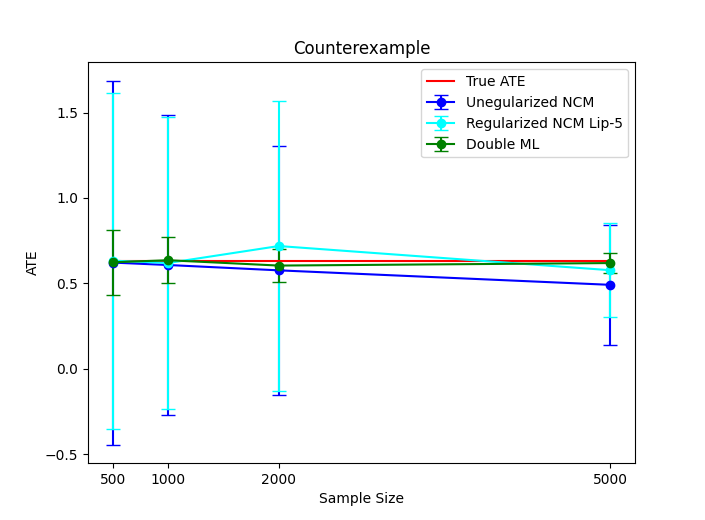
\includegraphics[width=\linewidth]{backdoor_counterexample0518.png}
    \end{minipage}
    \begin{minipage}{0.45\textwidth}
    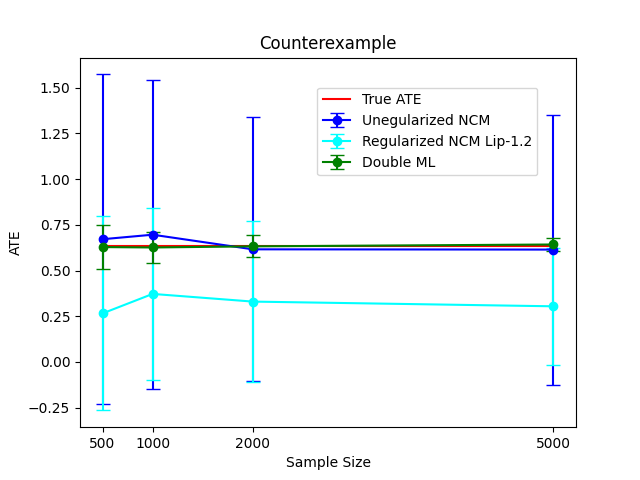
\includegraphics[width=\linewidth]{backdoor_counterexample1019.png}
    \end{minipage}
    \label{fig:counterexample}
    \caption{Comparison of Lipschitz regularized and unregularized neural causal algorithm. The two figures show the results of different architectures. The figure on the left side uses a medium-sized NN (width 128, depth 3) to approximate each structural function, while the right figure uses extremely small NNs (width 3, depth 1). In all experiments, we use the projected gradient to regularize the weight of the neural network. For each sample size, we repeat the experiment 5 times and take the average of the upper (lower) bound. }
\end{figure}


\section{Technical Lemmas}
\begin{lemma}\label{lemma:push-forward_err}
Let $\mu,\hat\mu$ be two measures on compact set $K\subset\mathbb R^{d_1}$, for any measurable functions $F,\hat F:K\rightarrow\mathbb R^{d_2}$, if $F$ is $L$-Lipschitz continuous, then
\begin{equation*}
W(F_{\#}\mu,\hat F_{\#}\hat\mu)\leqslant LW(\mu,\hat\mu)+d_2\|F-\hat F\|_\infty.
\end{equation*}
    \end{lemma}

\noindent\textit{Remark.} The measures $\mu$ and $\hat\mu$ are probability measures. The uniform infinity norm is $\|F-\hat F\|_\infty=\sup_{x\in K}\max_{j\in[d_2]}|F_j(x)-\hat F_j(x)|$.

    \begin{proof}
    For any $ 1$-Lipschitz function $ g:\mathbb{R}^{d_{2}}\rightarrow \mathbb{R}$,    
    \begin{align*}
    \mathbb{E}_{X\sim F_{\#} \mu }[ g( X)] -\mathbb{E}_{X\sim \hat{F}_{\#}\hat{\mu }}[ g( X)] & =\mathbb{E}_{X\sim \mu }[ g\circ F( X)] -\mathbb{E}_{X\sim \hat{\mu }}[ g\circ \hat{F}( X)]\\
     & =(\mathbb{E}_{X\sim \mu }[ g\circ F( X)] -\mathbb{E}_{X\sim \hat{\mu }}[ g\circ F( X)]) \\
     &\quad +(\mathbb{E}_{X\sim \hat{\mu }}[ g\circ F( X)] -\mathbb{E}_{X\sim \hat{\mu }}[ g\circ \hat{F}( X)]) .
    \end{align*}
Note that for any $x,y\in K$,
\begin{align*}
|g\circ F(x)-g\circ F(y)|\leqslant\|F(x)-F(y)\|\leqslant L\|x-y\|.
\end{align*}
Thus $g\circ F$ is $L$-Lipschitz continuous and
\begin{align}\label{eq:first_term}
\mathbb E_{X\sim\mu}[g\circ F(X)]-\mathbb E_{X\sim\hat\mu}[g\circ F(X)]\leqslant LW(\mu,\hat\mu).
\end{align}
For the second term,
\begin{align}\label{eq:second_term}
\mathbb E_{X\sim\hat\mu}[g\circ F(X)]-\mathbb E_{X\sim\hat\mu}[g\circ\hat F(X)]
&\leqslant\mathbb E_{X\sim\hat\mu}|g(F(X))-g(\hat F(X))|\notag\\
&\leqslant\mathbb E_{X\sim\hat\mu}\|F(X)-\hat F(X)\|\notag\\
&\leqslant\sup_{x\in K}\|F(x)-\hat F(x)\|\notag\\
&\leqslant d_2\|F-\hat F\|_\infty.
\end{align}
The last inequality follows by summing the $d_2$ coordinatewise bounds. If the uniform error is infinite, the asserted bound holds in the extended nonnegative reals.
    Combining (\ref{eq:first_term}) and (\ref{eq:second_term}) bounds the difference of expectations by $LW(\mu,\hat\mu)+d_2\|F-\hat F\|_\infty$ for every scalar $1$-Lipschitz function $g$. Taking the supremum over these functions gives the asserted bound for $W(F_{\#}\mu,\hat F_{\#}\hat\mu)$.
    \end{proof}


    \begin{lemma}\label{lemma:combin_err}
    Let $ \mu _{1} ,\cdots ,\mu _{n} ,\hat{\mu }_{1} ,\cdots ,\hat{\mu }_{n}$ be measure on $ \mathbb{R}^{d}$, for any $ p_{1} ,\cdots ,p_{n} \in [ 0,1]$ such that $ \sum _{k=1}^{n} p_{k} =1$, we have \begin{equation*}
    W\left(\sum _{k=1}^{n} p_{k} \mu _{k} ,\sum _{k=1}^{n} p_{k}\hat{\mu }_{k}\right) \leqslant \sum _{k=1}^{n} p_{k} W( \mu _{k} ,\hat{\mu }_{k}) .
    \end{equation*}

\emph{Additional condition.} For every $k\in[n]$, $\int_{\mathbb R^d}\|x\|\,\mu_k(dx)+\int_{\mathbb R^d}\|x\|\,\hat\mu_k(dx)<\infty$.
\end{lemma}

\noindent\textit{Remark.} For every $k\in[n]$, $\mu_k$ and $\hat\mu_k$ are probability measures on $\mathbb R^d$.

\noindent\textit{Remark (notation).} $\mu_n$ denotes the locally specified measure, with $n$ serving either as a component index or as the empirical sample size. In Lemma~\ref{lemma:combin_err}: $\mu_n$ is the component measure with index $n$ in the mixture, among measures $\mu_k$ on $\mathbb{R}^d$ for $k\in[n]$. In Lemma~\ref{lemma:product_err}: $\mu_n$ is the final component measure in the product $\mu=\mu_1\otimes\cdots\otimes\mu_n$. In Lemma~\ref{lemma:sup_wasserstein}: $\mu_n=n^{-1}\sum_{i=1}^n\delta_{X_i}$ is the empirical distribution of the sample with law $\mu$, on $\mathbb{R}^{d'}$.

    \begin{proof}
    For any $ 1$-Lipschitz function $ f:\mathbb{R}^{d}\rightarrow \mathbb{R}$, we have 
    \begin{align*}
    \mathbb{E}_{X\sim \sum _{k=1}^{n} p_{k} \mu _{k}}[ f( X)] -\mathbb{E}_{X\sim \sum _{k=1}^{n} p_{k}\hat{\mu }_{k}}[ f( X)] & =\sum _{k=1}^{n} p_{k}(\mathbb{E}_{X_{k} \sim \mu _{k}}[ f( X_{k})] -\mathbb{E}_{X_{k} \sim \hat{\mu }_{k}}[ f( X_{k})])\\
     & \leqslant \sum _{k=1}^{n} p_{k} W( \mu _{k} ,\hat{\mu }_{k}) .
    \end{align*}
    By dual formulation of Wasserstein-1 distance, 
    \begin{align*}
    W\left(\sum _{k=1}^{n} p_{k} \mu _{k} ,\sum _{k=1}^{n} p_{k} \mu _{k}\right) & =\sup _{f\ \text{1-Lipschitz}}\mathbb{E}_{X\sim \sum _{k=1}^{n} p_{k} \mu _{k}}[ f( X)] -\mathbb{E}_{X\sim \sum _{k=1}^{n} p_{k}\hat{\mu }_{k}}[ f( X)]\\
     & \leqslant \sum _{k=1}^{n} p_{k} W( \mu _{k} ,\hat{\mu }_{k}) .
    \end{align*}
    \end{proof}

    \begin{lemma}\label{lemma:product_err}
Given two measures $\mu=\mu_1\otimes\cdots\otimes\mu_n$, $\hat\mu=\hat\mu_1\otimes\cdots\otimes\hat\mu_n$, where every factor $\mu_k$ and $\hat\mu_k$ is a probability measure, we have
\begin{equation*}
W(\mu,\hat\mu)\leqslant\sum_{k=1}^n W(\mu_k,\hat\mu_k).
\end{equation*}
      \end{lemma}

\noindent\textit{Remark.} $W$ is Wasserstein-1 distance for the ground distance $\|x-y\|$. $S_\lambda(\mu,\nu)=W_{1,\lambda}(\mu,\nu)-\tfrac12W_{1,\lambda}(\mu,\mu)-\tfrac12W_{1,\lambda}(\nu,\nu)$.

      \begin{proof}
If $n=0$, both empty products are the probability measure on the one-point space and both sides are zero. Suppose $n\geqslant1$. If any $W(\mu_k,\hat\mu_k)=\infty$, the inequality holds in the extended nonnegative reals. Otherwise, for any $\epsilon>0$ and every $k\in[n]$, choose a probability coupling $\pi_k$ of $\mu_k$ and $\hat\mu_k$ such that
\begin{equation*}
\mathbb E_{(X_k,Y_k)\sim\pi_k}[\|X_k-Y_k\|_1]\leqslant W(\mu_k,\hat\mu_k)+\epsilon.
\end{equation*}
Such a coupling exists by the definition of the finite infimum defining $W$. Under the product probability law $\pi_1\otimes\cdots\otimes\pi_n$, put $X=(X_1,\ldots,X_n)$ and $Y=(Y_1,\ldots,Y_n)$. The marginal laws of $X$ and $Y$ are respectively $\mu$ and $\hat\mu$, because the coordinate pairs are independent and have the prescribed marginal laws. Thus this construction is a coupling of the product measures. The product $1$-norm is the sum of the coordinate $1$-norms, so
\begin{align*}
W(\mu,\hat\mu)
&\leqslant\mathbb E_{\pi_1\otimes\cdots\otimes\pi_n}[\|X-Y\|]\\
&=\sum_{k=1}^n\mathbb E_{(X_k,Y_k)\sim\pi_k}[\|X_k-Y_k\|_1]\\
&\leqslant\sum_{k=1}^n W(\mu_k,\hat\mu_k)+n\epsilon.
\end{align*}
Letting $\epsilon\downarrow0$ proves the result.
      \end{proof}

    \begin{lemma}[Approximation error of Gumbel-Softmax layer]\label{lemma:gumbel_err}
        Given $1 >\tau  >0$ and $p_{1} ,\cdots ,p_{n}  >0$, let $\mu ^{\tau } \sim X^{\tau } =\left( X_{1}^{\tau } ,\cdots ,X_{n}^{\tau }\right)$ be 
\begin{equation}
X_{k} =\frac{\exp((\log p_{k} +G_{k}) /\tau )}{\sum _{k=1}^{n}\exp((\log p_{k} +G_{k}) /\tau )} ,\label{eq:gumbel}
\end{equation}
where $G_{k} \sim \exp( -x-\exp( -x))$ are i.i.d. standard Gumbel variables. Let $\mu ^{0}$ be the distribution of $X^{0} =\lim _{\tau \rightarrow 0} X^{\tau } =\left( X_{1}^{0} ,\cdots ,X_{n}^{0}\right)$. Then,  
\begin{equation*}
W\left( \mu ^{\tau } ,\mu ^{0}\right) \leqslant 2( n-1) \tau -2n( n-1) e^{-1} \tau \log \tau .
\end{equation*}
    \end{lemma}

\noindent\textit{Remark.} The gap event is $E_\delta=\{\exists\,1\leqslant i<j\leqslant n:|G_i+\log p_i-G_j-\log p_j|<\delta\}$, and its union bound counts each unordered pair once. In the displayed softmax formula, $X_k$ means $X_k^\tau$, $\mu^\tau=P(X^\tau)$, and $X^0=\lim_{\tau\downarrow0}X^\tau$ almost surely with the same i.i.d. standard Gumbel variables $G_1,\ldots,G_n$ used for every $\tau$.

\noindent\textit{Remark (notation).} $X^\tau$ uses positive weights $p_1,\ldots,p_n$, which need not sum to one, and $0<\tau<1$, with coordinates indexed by $k\in[n]$; all coordinates are positive and sum to one. In Theorem~\ref{thm:wide_nn}, the result split from Theorem~\ref{thm:wide_nn}: In the mixing construction, $n=N_C$ and $p_i=\mathbb{P}(C_i)>0$ for $i\in[N_C]$; $X^\tau$ is the vector of Gumbel-softmax weights assigned to these support components. $X^0=\lim_{\tau\downarrow0}X^\tau=e_I$ almost surely, where $I=\arg\max_{k\in[n]}(\log p_k+G_k)$, using the same Gumbel draws throughout the limit; ties may be assigned to the first maximizing coordinate. In Theorem~\ref{thm:wide_nn}, the result split from Theorem~\ref{thm:wide_nn}: In the mixing construction, $n=N_C$ and $p_i=\mathbb{P}(C_i)>0$ for $i\in[N_C]$; $X^0$ is the one-hot limit of these component weights, with $P(X^0=e_i)=\mathbb{P}(C_i)$. $\mu^0$ is the law of the one-hot vector $X^0$, supported on the vertices of $\Delta_n$, with $\mu^0(\{e_k\})=p_k/\sum_{j=1}^n p_j$ for $k\in[n]$.


    \begin{proof}
    Without loss of generality, we may assume that $\sum _{k=1}^{n} p_{k} =1$. Otherwise, we can divide the denominator and numerator in (\ref{eq:gumbel}) by $\sum _{k=1}^{n} p_{k}$. Let $\Delta _{n} =\left\{( x_{1} ,\cdots ,x_{n}) :\sum _{k=1}^{n} x_{k} =1\right\}$. We construct a transportation map $T:\Delta _{n}\rightarrow \Delta _{n}$ as follows. $T( x_{1} ,\cdots ,x_{n})$ is a $n$-dimensional vector with all zeros except that the $i=\arg\max_{j} x_{j}$-th entry being one. If there are multiple coordinates that is maximum, we choose the first coordinate and let the remaining coordinate be zero. It is easy to verify that $T_{\#} \mu ^{\tau }$ and $\mu ^{0}$ have the same distribution \cite{maddisonConcreteDistributionContinuous2017}.
 For any $\delta  >0$, we have 
\begin{align*}
P( |G_{k_{1}} +\log p_{k_{1}} -( G_{k_{2}} +\log p_{k_{2}}) |< \delta ) & =\int _{-\infty }^{\infty }\int _{y+\log\frac{p_{k2}}{p_{k_{1}}} -\delta }^{y+\log\frac{p_{k2}}{p_{k_{1}}} +\delta }\exp( -x-y-\exp( -y) -\exp( -x)) dxdy\\
 & \leqslant 2\delta e^{-1}\int _{-\infty }^{\infty }\exp( -y-\exp( -y)) dy=2\delta ,
\end{align*}where we have used $\exp( -x-\exp( -x)) \leqslant \exp( -1)$. Let event $E_{\delta } =\{\exists i,j\in [ n] :|G_{i} +\log p_{i} -( G_{j} +\log p_{j}) |< \delta \}$, we have 
\begin{align*}
P( E_{\delta }) & \leqslant \sum _{i\neq j}P( |G_{i} +\log p_{i} -( G_{j} +\log p_{j}) |< \delta )\\
 & \leqslant \delta n( n-1) e^{-1} .
\end{align*}Now, we calculate the transportation cost 
\begin{align*}
\mathbb{E}_{X^{\tau } \sim \mu ^{\tau }}\left[ \| T\left( X^{\tau }\right) -X^{\tau } \| _{1}\right] & \leqslant P( E_{\delta })\mathbb{E}_{X^{\tau } \sim \mu ^{\tau }}\left[ \| T\left( X^{\tau }\right) -X^{\tau } \| _{1} |E_{\delta }\right] +P\left( E_{\delta }^{c}\right)\mathbb{E}_{X^{\tau } \sim \mu ^{\tau }}\left[ \| T\left( X^{\tau }\right) -X^{\tau } \| _{1} |E_{\delta }^{c}\right] .
\end{align*}Note that $\| T\left( X^{\tau }\right) -X^{\tau } \| _{1} \leqslant 2$. For the first term, we have 
\begin{equation*}
P( E_{\delta })\mathbb{E}_{X^{\tau } \sim \mu ^{\tau }}\left[ \| T\left( X^{\tau }\right) -X^{\tau } \| _{1} |E_{\delta }\right] \leqslant 2\delta n( n-1) e^{-1} .
\end{equation*}For the second term, under event $E_{\delta }^{c}$, let $k_{\max} =\arg\max_{i} X_{i}$, if $j=k_{\max} =\arg\max_{i}(\log p_{k} +G_{k})$
\begin{align*}
\Bigl|\frac{\exp((\log p_{j} +G_{j}) /\tau )}{\sum _{k=1}^{n}\exp((\log p_{k} +G_{k}) /\tau )} -1\Bigl| & =\Bigl|\frac{\sum _{k\neq j}\exp((\log p_{k} +G_{k}) /\tau )}{\sum _{k=1}^{n}\exp((\log p_{k} +G_{k}) /\tau )}\Bigl|\\
 & \leqslant \Bigl|\frac{\sum _{k\neq j}\exp((\log p_{k} +G_{k}) /\tau )}{\exp((\log p_{j} +G_{j}) /\tau )}\Bigl|\\
 & =\sum _{k\neq j}\exp((\log p_{k} +G_{k} -(\log p_{j} +G_{j})) /\tau )\\
 & \leqslant ( n-1)\exp( -\delta /\tau ) .
\end{align*}If $j\neq k_{\max}$, we have 
\begin{align*}
\Bigl|\frac{\exp((\log p_{j} +G_{j}) /\tau )}{\sum _{k=1}^{n}\exp((\log p_{k} +G_{k}) /\tau )}\Bigl| & \leqslant \exp((\log p_{j} +G_{j} -(\log p_{\max} +G_{\max})) /\tau ) \leqslant \exp( -\delta /\tau ) .
\end{align*}
Therefore, 
\begin{align*}
\mathbb{E}_{X^{\tau } \sim \mu ^{\tau }}\left[ \| T\left( X^{\tau }\right) -X^{\tau } \| _{1} |E_{\delta }^{c}\right] & \leqslant 2( n-1)\exp( -\delta /\tau ) .
\end{align*}We get an upper bound of the transportation cost,
\begin{equation*}
W\left( \mu ^{\tau } ,\mu ^{0}\right) \leqslant \mathbb{E}_{X^{\tau } \sim \mu ^{\tau }}\left[ \| T\left( X^{\tau }\right) -X^{\tau } \| _{1}\right] \leqslant 2\delta n( n-1) e^{-1} +2( n-1)\exp( -\delta /\tau ) .
\end{equation*}Let $\delta =-\tau \log \tau $, we get 
\begin{equation*}
W\left( \mu ^{\tau } ,\mu ^{0}\right) \leqslant 2( n-1) \tau -2n( n-1) e^{-1} \tau \log \tau .
\end{equation*}
\end{proof}

\begin{lemma}[Approximation Error of Sinkhorn distance]\label{lemma:sinkhorn_approx}
For any $\mu\in\Delta_n$, $\nu\in\Delta_m$, and $\lambda>0$, let $\mu$ and $\nu$ be the weights of finite probability measures on points $x_1,\ldots,x_n$ and $y_1,\ldots,y_m$ in a common Euclidean space with the paper's $1$-norm. Put $c_{ij}=\|x_i-y_j\|$ and

\[
\Pi(\mu,\nu)=\left\{T\in[0,\infty)^{n\times m}:\sum_jT_{ij}=\mu_i,\ \sum_iT_{ij}=\nu_j\right\},\qquad h(T)=1-\sum_{i,j}T_{ij}\log T_{ij},
\]

with $0\log0=0$. Here the entropy regularized Wasserstein-1 distance is

\[
W_{1,\lambda}(\mu,\nu)=\min_{T\in\Pi(\mu,\nu)}\left\{\sum_{i,j}c_{ij}T_{ij}-\lambda h(T)\right\},
\]

and $W(\mu,\nu)=\min_{T\in\Pi(\mu,\nu)}\sum_{i,j}c_{ij}T_{ij}$. Then
\begin{align*}
-(\log(mn)+1)\lambda\leqslant W_{1,\lambda}(\mu,\nu)-W(\mu,\nu)\leqslant0.
\end{align*} Moreover, we have the following estimation of approximation error.  
\begin{align*}
|S_{\lambda }( \mu ,\nu ) -W( \mu ,\nu ) | & \leqslant 2(\log( mn) +1) \lambda .
\end{align*}
\end{lemma}

\noindent\textit{Remark.} The self terms in $S_\lambda(\mu,\nu)=W_{1,\lambda}(\mu,\nu)-\tfrac12W_{1,\lambda}(\mu,\mu)-\tfrac12W_{1,\lambda}(\nu,\nu)$ use the same $1$-norm ground distance on the corresponding support points.

\noindent\textit{Remark (notation).} $W_{1,\lambda}$ uses the supplied finite support points, the paper's $1$-norm ground cost, and the entropy subtraction $-\lambda h(T)$ with $h(T)=1-\sum_{i,j}T_{ij}\log T_{ij}$ and $0\log0=0$.

\begin{proof}
The transportation polytope is nonempty and compact, and both objectives are continuous under $0\log0=0$, so their minima exist. Let $T^*$ minimize the unregularized transport cost and let $T_\lambda$ minimize the regularized objective. Since $h(T)\geqslant0$ for every probability plan,

\[
W_{1,\lambda}(\mu,\nu)\leqslant\sum_{i,j}c_{ij}T^*_{ij}-\lambda h(T^*)\leqslant W(\mu,\nu).
\]

Also $\sum_{i,j}c_{ij}(T_\lambda)_{ij}\geqslant W(\mu,\nu)$. It follows that
\begin{align}\label{eq:err_reg_wass}
-\lambda\max_{T\in\Pi(\mu,\nu)}h(T)\leqslant W_{1,\lambda}(\mu,\nu)-W(\mu,\nu)\leqslant0.
\end{align} Since $ T_{ij} \in [ 0,1]$ and $ f( x) =-x\log x$ is concave, we have 
\begin{align*}
h( T) = & -nm\cdot \frac{1}{nm}\sum _{i,j=1}^{n,m} T_{ij}\log T_{ij} +1.\\
 & \leqslant -nm\cdot \left(\frac{1}{nm}\sum _{i,j=1}^{n,m} T_{ij}\right)\log\left(\frac{1}{nm}\sum _{i,j=1}^{n,m} T_{ij}\right) +1\\
 & =1+\log( nm) .
\end{align*}
By definition of Sinkhorn distance, 
\begin{align*}
S_{\lambda }( \mu ,\nu ) & = W_{1,\lambda }( \mu ,\nu ) -W_{1,\lambda }( \mu ,\mu )/2 -W_{1,\lambda }( \nu ,\nu )/2 .
\end{align*}
Let $a=W_{1,\lambda}(\mu,\nu)-W(\mu,\nu)$, $b=W_{1,\lambda}(\mu,\mu)$, and $c=W_{1,\lambda}(\nu,\nu)$. The self-transport Wasserstein costs are zero. By (\ref{eq:err_reg_wass}) and the entropy calculation,

\[
|a|\leqslant(1+\log(nm))\lambda,\quad |b|\leqslant(1+2\log n)\lambda,\quad |c|\leqslant(1+2\log m)\lambda.
\]

Consequently
\begin{align*}
|S_\lambda(\mu,\nu)-W(\mu,\nu)|
&=|a-b/2-c/2|\\
&\leqslant|a|+|b|/2+|c|/2\\
&\leqslant2(1+\log(nm))\lambda.
\end{align*}
\end{proof}

\begin{lemma}\label{lemma:sup_wasserstein}
Given a probability measure $\mu$ on $\mathbb R^{d'}$ and a class $\mathcal F$ of measurable functions $f:\mathbb R^{d'}\rightarrow\mathbb R^d$, suppose that each scalar coordinate class $\mathcal F_j=\{x\mapsto f_j(x):f\in\mathcal F\}$, $j\in[d]$, has pseudo-dimension less than $d_{\mathcal F}<\infty$ and there exists $K>0$ such that $\|f(x)\|_\infty\leqslant K$ for all $f\in\mathcal F$ and $x\in\mathbb R^{d'}$. Suppose in addition that there are a standard Borel space $T$ and a jointly Borel map $G:T\times\mathbb R^{d'}\rightarrow[-K,K]^d$ such that $\mathcal F=\{G(t,\cdot):t\in T\}$. There are positive constants $C,c$ depending only on $d,K$ such that, with probability at least

\[
1-\exp\left(C\left((1+\delta^{-d})\log(2+\delta^{-1})+d_{\mathcal F}\log(2+\epsilon^{-1})\right)-cn\epsilon^2\right),
\]

\begin{align*}
\sup_{f\in\mathcal F}W(f_{\#}\mu,f_{\#}\mu_n)\leqslant\delta+\epsilon
\end{align*}
for all $\delta,\epsilon>0$, where $\mu_n$ is the empirical distribution of $\mu$. 
\end{lemma}

\noindent\textit{Remark.} A network in $\mathcal{NN}_{k_1,k_2}(W,L)$ has $L$ hidden layers, each of width at most $W$, followed by the affine output layer (width at most $W$ and exactly $W$ give the same class of functions: a narrower layer is padded with zero units). The covering number $\mathcal{N}(\epsilon,S,\|\cdot\|_1)$ is that of the cited source (Anthony and Bartlett): the least size of a subset $C\subseteq S$ such that every point of $S$ lies at $\ell_1$ distance strictly less than $\epsilon$ from some point of $C$. The probability bound is for each fixed pair $\delta,\epsilon>0$. Probabilities of uniform deviation events are evaluated in the completion of the sample law. The boundedness condition means $\|f(x)\|_{\infty}\leqslant K$ for every $f\in\mathcal{F}$ and $x\in\mathbb{R}^{d'}$.

\noindent\textit{Remark (notation).} $d_{\mathcal F}<\infty$ is a strict upper bound on the pseudo-dimensions of the scalar function classes specified in its local use. In Lemma~\ref{lemma:sup_wasserstein}: For every $j\in[d]$, $\mathcal F_j=\{x\mapsto f_j(x):f\in\mathcal F\}$ satisfies $\operatorname{Pdim}(\mathcal F_j)<d_{\mathcal F}$; the bound applies separately to each coordinate class.

\begin{proof}
The empty class satisfies the uniform assertion vacuously, so assume $T\ne\varnothing$. Let $X_1,\ldots,X_n$ be independent observations with law $\mu$. By the dual formulation of Wasserstein distance,
\begin{align*}
\sup_{f\in\mathcal F}W(f_{\#}\mu,f_{\#}\mu_n)
=\sup_{h\in\mathcal H}\sup_{f\in\mathcal F}\left(\mathbb E_{X\sim\mu_n}h(f(X))-\mathbb E_{X\sim\mu}h(f(X))\right),
\end{align*}
where

\[
\mathcal H=\{h:[-K,K]^d\rightarrow\mathbb R:h(0)=0,\ |h(x)-h(y)|\leqslant\|x-y\|\}.
\]

Every such $h$ takes values in $[-dK,dK]$. Retain the unnormalized empirical covering number
\begin{align*}
\mathcal N_1(r,\mathcal F,N)=\sup_{x_1,\ldots,x_N}\mathcal N\left(r,\{(f(x_1),\ldots,f(x_N)):f\in\mathcal F\},\|\cdotp\|_1\right),
\end{align*}
where the $1$-norm on the evaluation vector sums over all sample points and output coordinates. 

With the uniform norm, $\mathcal H$ is closed, uniformly bounded and equicontinuous on the compact cube, hence is a compact metric space by Arzela--Ascoli. Evaluation $(h,y)\mapsto h(y)$ is continuous: its increment is bounded by $\|h-h'\|_\infty+\|y-y'\|$. Consequently $(t,h,x)\mapsto h(G(t,x))$ is jointly Borel on $T\times\mathcal H\times\mathbb R^{d'}$. Its bounded population integral is Borel in $(t,h)$: this holds for indicators of measurable rectangles, is preserved by bounded monotone limits and linear combinations, and extends to bounded Borel functions by the monotone class theorem. Every strict deviation event is the projection of a Borel set from this standard Borel parameter space and is therefore analytic and universally measurable; weak supremum events are countable intersections of strict ones. The same reasoning applies to two samples and finite coordinate swaps. All probabilities below are thus defined in the completion of the sample law. Obviously, if $ h$ is 1-Lipschitz, 
\begin{align*}
\mathcal{N}_{1}( \epsilon ,h\circ \mathcal{F} ,n) & \leqslant \mathcal{N}_{1}( \epsilon ,\mathcal{F} ,n) .
\end{align*}
Put $v=\lfloor d_{\mathcal F}\rfloor$. Each coordinate class has pseudo-dimension at most $v$. Normalize its range by $f_j\mapsto(f_j+K)/(2K)$. Applying Theorem 18.4 of \cite{anthony1999neural} in its averaged empirical metric, and then undoing the normalization, bounds a scalar unnormalized cover of radius $r/(2d)$ on $N$ points by

\[
e(v+1)\left(2+\frac{8eKdN}{r}\right)^v.
\]

The additional $2$ allows radii beyond the normalized unit range. Take the product of these $d$ covers. For every product ball meeting the evaluation vectors of $\mathcal F$, choose one such vector as its center. Two vectors in that product ball differ by at most $r/d$ in each scalar unnormalized metric, hence by at most $r$ in the summed vector metric. Thus

\[
\mathcal N_1(r,\mathcal F,N)\leqslant\left[e(v+1)\left(2+\frac{8eKdN}{r}\right)^v\right]^d.
\]

This exhibits both sample-size and range scaling. 

Fix $h\in\mathcal H$, and define

\[
a_f(x)=\frac{h(f(x))+dK}{2dK},\qquad z_f(x)=\sqrt{a_f(x)}.
\]

Both functions take values in $[0,1]$. On $N$ points, the inequality $|\sqrt a-\sqrt b|\leqslant\sqrt{|a-b|}$ and the Cauchy--Schwarz inequality give

\[
\frac1N\sum_{i=1}^N|z_f(x_i)-z_g(x_i)|\leqslant\left(\frac{1}{2dKN}\sum_{i=1}^N\|f(x_i)-g(x_i)\|\right)^{1/2}.
\]

Consequently an unnormalized vector cover of radius $2dKNr^2$ gives an averaged scalar cover of the class $\{z_f:f\in\mathcal F\}$ of radius $r$, whose cardinality is at most

\[
\left[e(v+1)(2+4e/r^2)^v\right]^d.
\]

By Theorem 17.1 in \cite{anthony1999neural}, with its standing measurability condition, let $X$ and $T_0$ be standard Borel spaces, let $g:T_0\times X\rightarrow[0,1]$ be jointly Borel, and put $\mathcal G=\{g(t,\cdot):t\in T_0\}\ne\varnothing$. For every Borel probability distribution $P$ on $X\times[0,1]$, every $0<\zeta<1$ and every positive integer $m$,

\[
P^m\left\{\text{some }t\in T_0\text{ has }\left|\mathbb E_{(x,y)\sim P}(g(t,x)-y)^2-\frac1m\sum_{i=1}^m(g(t,x_i)-y_i)^2\right|\geqslant\zeta\right\}
\leqslant4\mathcal N_1^{\mathrm{avg}}(\zeta/16,\mathcal G,2m)\exp(-\zeta^2m/32).
\]

Here the draws are independent, the probability is taken in the completed sample law, and $\mathcal N_1^{\mathrm{avg}}$ uses the averaged empirical metric. For the present class, $(t,x)\mapsto\sqrt{(h(G(t,x))+dK)/(2dK)}$ is jointly Borel, since $h$ is continuous and the square root is continuous on $[0,1]$. Its parameter space is the same standard Borel space $T$, and its constant-response input law is $\mu\otimes\delta_0$. Apply this form of Theorem 17.1 to the class with response identically zero. Its squared loss is $z_f^2=a_f$. For $0<\epsilon<2dK$, put $\eta=\epsilon/(2dK)$ and use the averaged cover at radius $\eta/16$ on $2n$ points. The theorem gives

\[
\mathbb P\left(\sup_{f\in\mathcal F}|(\mu_n-\mu)(h\circ f)|>\epsilon\right)
\leqslant4\left[e(v+1)(2+1024e/\eta^2)^v\right]^d\exp(-n\eta^2/32).
\]

Since $v\leqslant d_{\mathcal F}$ and $\log(v+1)\leqslant v$, the logarithm of the right-hand side is bounded by $C_0+C_1d_{\mathcal F}\log(2+\epsilon^{-1})-c_1n\epsilon^2$, with constants depending only on $d,K$. If $\epsilon\geqslant2dK$, the deviation is deterministically at most $2dK$, and the desired deviation bound is immediate.
Let $\mathcal H_\delta$ be a finite $\delta/2$-net of $\mathcal H$ in the uniform norm. Such a net has

\[
\log|\mathcal H_\delta|\leqslant C_2(1+\delta^{-d})\log(2+\delta^{-1}),
\]

where $C_2$ depends only on $d,K$. To see this, take a grid in $[-K,K]^d$ with $1$-norm mesh at most $\delta/8$ and at most $(1+C_3/\delta)^d$ points. Quantize the values of $h$ at these points into bins of width at most $\delta/8$ in $[-dK,dK]$. There are at most $2+C_4/\delta$ bins at each point. Choose one member of $\mathcal H$ from each nonempty quantization pattern. Two functions with the same pattern differ by at most $\delta/8$ at grid points and by at most $3\delta/8$ everywhere, using their Lipschitz bounds and a nearest grid point. These representatives form the required net. Counting patterns gives the displayed entropy bound. Apply the fixed-$h$ concentration bound to every $h\in\mathcal H_\delta$ and take a union bound. For $0<\epsilon<2dK$, after enlarging a constant depending only on $d,K$,

\[
\mathbb P\left(\sup_{h\in\mathcal H_\delta,f\in\mathcal F}(\mu_n-\mu)(h\circ f)>\epsilon\right)
\leqslant\exp\left(C\left((1+\delta^{-d})\log(2+\delta^{-1})+d_{\mathcal F}\log(2+\epsilon^{-1})\right)-cn\epsilon^2\right).
\]

For every $h\in\mathcal H$, choose $\tilde h\in\mathcal H_\delta$ with $\|h-\tilde h\|_\infty\leqslant\delta/2$. Since $\mu_n$ and $\mu$ are probability measures,

\[
|(\mu_n-\mu)((h-\tilde h)\circ f)|\leqslant\delta.
\]

Therefore

\[
\sup_{h\in\mathcal H,f\in\mathcal F}(\mu_n-\mu)(h\circ f)
\leqslant\delta+\sup_{\tilde h\in\mathcal H_\delta,f\in\mathcal F}(\mu_n-\mu)(\tilde h\circ f).
\]

The dual formula yields the stated Wasserstein bound. If $\epsilon\geqslant2dK$, both push-forward measures are supported in a set of $1$-norm diameter $2dK$, so their Wasserstein distance is at most $2dK\leqslant\delta+\epsilon$ deterministically. This completes the proof for all positive $\delta,\epsilon$.
\end{proof}
By Theorem 18.4 in \cite{anthony1999neural}, if $\mathcal G$ is a nonempty class of functions from a set $X$ into $[0,1]$ with finite pseudo-dimension $v$, then for every $0<\epsilon\leqslant1$ and every positive integer $m$,
\begin{align*}
\mathcal{N}_{1}^{\mathrm{avg}}(\epsilon,\mathcal G,m)\leqslant\mathcal{M}_{1}^{\mathrm{avg}}(\epsilon,\mathcal G,m)<e(v+1)\left(\frac{2e}{\epsilon}\right)^{v},
\end{align*}
where $\mathcal{N}_{1}^{\mathrm{avg}}(\epsilon,\mathcal G,m)$ and $\mathcal{M}_{1}^{\mathrm{avg}}(\epsilon,\mathcal G,m)$ are the largest, over $x_1,\ldots,x_m\in X$, covering and packing numbers of $\{(g(x_1),\ldots,g(x_m)):g\in\mathcal G\}$ in the averaged metric $d_1(u,w)=\frac1m\sum_{i=1}^m|u_i-w_i|$. 

This is Theorem 18.4 in \cite{anthony1999neural}.

The cited assertion used in Lemma~\ref{lemma:sup_wasserstein} is the following restricted form of Theorem 17.1 in \cite{anthony1999neural}, with its standing measurability condition. Let $X$ and $T$ be standard Borel spaces, let $g:T\times X\rightarrow[0,1]$ be jointly Borel, and put $\mathcal G=\{g(t,\cdot):t\in T\}\ne\varnothing$. For every Borel probability distribution $P$ on $X\times[0,1]$, every $0<\epsilon<1$ and every positive integer $m$,

\[
\begin{aligned}
&P^m\left\{\text{some }t\in T\text{ has }\left|\mathbb E_{(x,y)\sim P}(g(t,x)-y)^2-\frac1m\sum_{i=1}^m(g(t,x_i)-y_i)^2\right|\geqslant\epsilon\right\}\\
&\quad\leqslant4\mathcal N_1^{\mathrm{avg}}(\epsilon/16,\mathcal G,2m)\exp(-\epsilon^2m/32).
\end{aligned}
\]

Here the sample consists of independent draws from $P$, the probability is taken in its completion, and $\mathcal N_1^{\mathrm{avg}}(r,\mathcal G,N)$ is the supremum over $x_1,\ldots,x_N\in X$ of the covering number of the evaluation vectors in the metric $N^{-1}\sum_i|u_i-v_i|$. This structural domain supplies the standing measurability condition: the loss is bounded and jointly Borel, and its integral against $P$ is Borel in $t$. The latter assertion holds for indicators of measurable rectangles, is preserved by bounded monotone limits and linear combinations, and hence holds for bounded Borel functions by the monotone class theorem. Each bad event is a projection of a Borel subset of $T\times(X\times[0,1])^m$, so it is analytic and universally measurable. Replacing the sample by two independent samples or applying any of the finitely many coordinate swaps gives Borel functions on finite products and therefore the same measurability conclusion. Thus the sample and ghost-sample events used by Theorem 17.1 are measurable in the completed sample laws, and that theorem gives the displayed inequality.

\noindent\textit{Remark (notation).} $\mathcal{N}_1(\epsilon,\mathcal{F},n)=\sup_{x_1,\ldots,x_n}\mathcal{N}(\epsilon,\{(f(x_1),\ldots,f(x_n)):f\in\mathcal{F}\},\|\cdot\|_1)$, where the points range over the domain of $\mathcal{F}$ and the norm is the printed $\ell_1$ norm without a factor $1/n$. In a result cited in the proof of Lemma~\ref{lemma:sup_wasserstein}: $\mathcal N_1^{\mathrm{avg}}(\epsilon,\mathcal G,m)$ is the supremum over $x_1,\ldots,x_m\in X$ of the covering numbers of $\{(g(x_1),\ldots,g(x_m)):g\in\mathcal G\}$ in $d_1(u,w)=m^{-1}\sum_{i=1}^m|u_i-w_i|$, for $\epsilon>0$ and positive integers $m$. This averaged covering number is distinct from the covering number defined with the unnormalized $\ell_1$ norm. In a result cited in the proof of Lemma~\ref{lemma:sup_wasserstein}: $\mathcal N_1^{\mathrm{avg}}(r,\mathcal G,N)$ is the supremum over $x_1,\ldots,x_N\in X$ of the covering number of $\{(g(x_1),\ldots,g(x_N)):g\in\mathcal G\}$ in $d_1(u,w)=N^{-1}\sum_{i=1}^N|u_i-w_i|$. The probability bound uses $r=\epsilon/16$ and $N=2m$. This averaged covering number is distinct from the covering number defined with the unnormalized $\ell_1$ norm. $\mathcal H_\delta\subseteq\mathcal H$ is a finite $\delta/2$-net in the uniform norm of $\mathcal H=\{h:[-K,K]^d\rightarrow\mathbb R:h(0)=0,\ |h(x)-h(y)|\leqslant\|x-y\|\}$, for $\delta>0$.



\end{document}